\documentclass[11pt]{memoir}

\def\watermarkloaded{0}

\def\Title{A Wildness of the Heart}
\def\FullTitle{\Title}
\def\AuthorFirst{Madison}
\def\AuthorLast{Scott-Clary}
\def\AuthorFull{\AuthorFirst\ \AuthorLast}
\def\Illustrator{Artist}
\def\IllustratorWeb{www.patreon.com/artist}

\def\Edition{First}
\def\EditionsList{10 9 8 7 6 5 4 3 2 1}
\def\Year{2021}

\def\ISBN{XXX-X-XXXXXX-XX-X}

\def\Publisher{PUBLISHER}
\def\PublisherEmail{publisher@example.com}
\def\PublisherURL{example.com}
\def\PublisherLocation{City, STATE}

%%% Watermark for draft
\usepackage{draftwatermark}
\def\watermarkloaded{1}
\SetWatermarkLightness{0.9}

%

%%% Resets
% memoir defines footruleskip, we want fancyhdr's
\let\footruleskip\undefined
\DisemulatePackage{setspace}

%%% Hyperref warning suppression
% I want math symbols, hyperref complains
% must be before hyperref included
\usepackage{silence}
\WarningFilter[pdftoc]{hyperref}{Token not allowed in a PDF string}
\ActivateWarningFilters[pdftoc]

%%% Package imports not needing expansion
\usepackage{graphicx}
\usepackage{hyperref}
\usepackage{setspace}
\usepackage{xifthen}
\usepackage{xltxtra}
\usepackage{verse}
\usepackage{paracol}
\usepackage{marginnote}
\renewcommand*{\marginnotevadjust}{0.75ex}
\setlength{\columnsep}{0pt}

%%% Headers and page styles
\usepackage[pagestyles]{titlesec}
\usepackage{fancyhdr}
\setlength{\headheight}{15.2pt}

% ourbook style with fancy headers and chapter headings
\fancypagestyle{ourbook}{
  % headers
  \renewcommand{\headrulewidth}{0pt}
  \renewcommand{\printchaptername}{}
  \renewcommand{\chapternamenum}{}
  \renewcommand{\printchapternum}{}
  \renewcommand{\printchaptertitle}[1]{%
  \TitleFont\huge ##1}
  \setsecheadstyle{\TitleFont}
  \renewcommand{\partnamefont}{\DisplayFont\huge}
  \renewcommand{\partnumfont}{\DisplayFont\huge}
  \renewcommand{\parttitlefont}{\DisplayFont\Huge}
  \renewcommand{\chaptername}{}
  \renewcommand{\thechapter}{}
  \setlength{\parskip}{0pt}
  \fancyhf{}
  \fancyhf[FRO,FLE]{\thepage}
  \fancyhf[HRO]{\tiny\DisplayFont\leftmark}
  \fancyhf[HLE]{\tiny\DisplayFont\rightmark}
}

% plain style with only page num
\fancypagestyle{plain}{
  \fancyhf{}
  \renewcommand{\headrulewidth}{0pt}
  \renewcommand{\footrulewidth}{0pt}
  %\fancyhf[FRO,FLE]{\thepage}
}

% single space after periods
\frenchspacing

% Attempt justification at all costs
\sloppy

% Widows and orphans
\widowpenalty=10000
\clubpenalty=10000

% page sizes for trade paperback
\usepackage[
  paperwidth=6in,
  paperheight=9in,
  layoutwidth=6in,
  layoutheight=9in,
  vmargin=0.5in,
  outer=0.5in,
  inner=1.1in,
  includeheadfoot,
  twoside,
  showcrop
]{geometry}
\ifdefined\SetWatermarkHorCenter
  \SetWatermarkHorCenter{3in}
  \SetWatermarkVerCenter{4.5in}
\fi


%%% ToC munging
% Remove ToC header
\renewcommand{\contentsname}{}
\renewcommand{\cftdot}{\small{$\cdot$}}
\renewcommand{\cftchapterdotsep}{3}
\renewcommand{\cftsectiondotsep}{10000}
% start toc at top of page
\renewcommand*\tocheadstart{}{}
\hypersetup{final}

%%% Font
% Uncomment and modify to your font specs

\usepackage{fontspec}
\setmainfont{Gentium Book Basic}
\newfontfamily\TitleFamily{Tom's New Roman}
\newfontface\TitleFont{Tom's New Roman}
\newfontfamily\HeaderFamily{Gentium Basic}
\newfontface\HeaderFont{Gentium Basic}
\newfontface\ChapterFont{Spectral}
\newfontfamily\TocFont{Gentium Basic Bold}
\newfontfamily\SmileyFont{DejaVu Sans}

%%% Title page
\title{\TitleFont{\FullTitle}\\ \vspace{1cm}\large\Subtitle\vfill\null}
\author{\DisplayFont{\AuthorFull}}
\date{}

%%% Section divider
% don't forget to \noindent the line after!
\renewcommand\rule[2]{$\star$}
\newcommand\secdiv{
  \begin{center}
    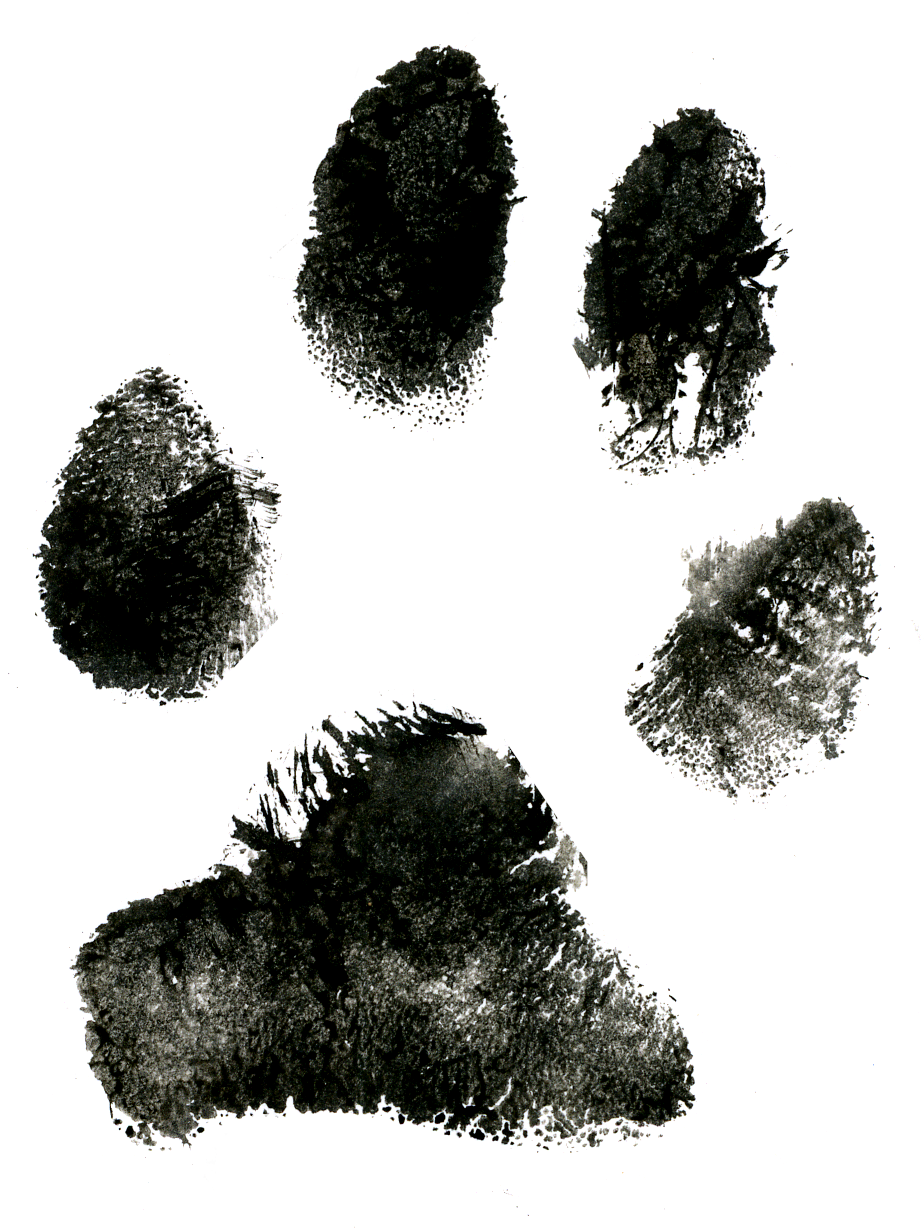
\includegraphics[width=0.5cm]{assets/zpaw.png}
  \end{center}
}

\newcommand\storydiv{
  \begin{center}
    \null
    \vfill
    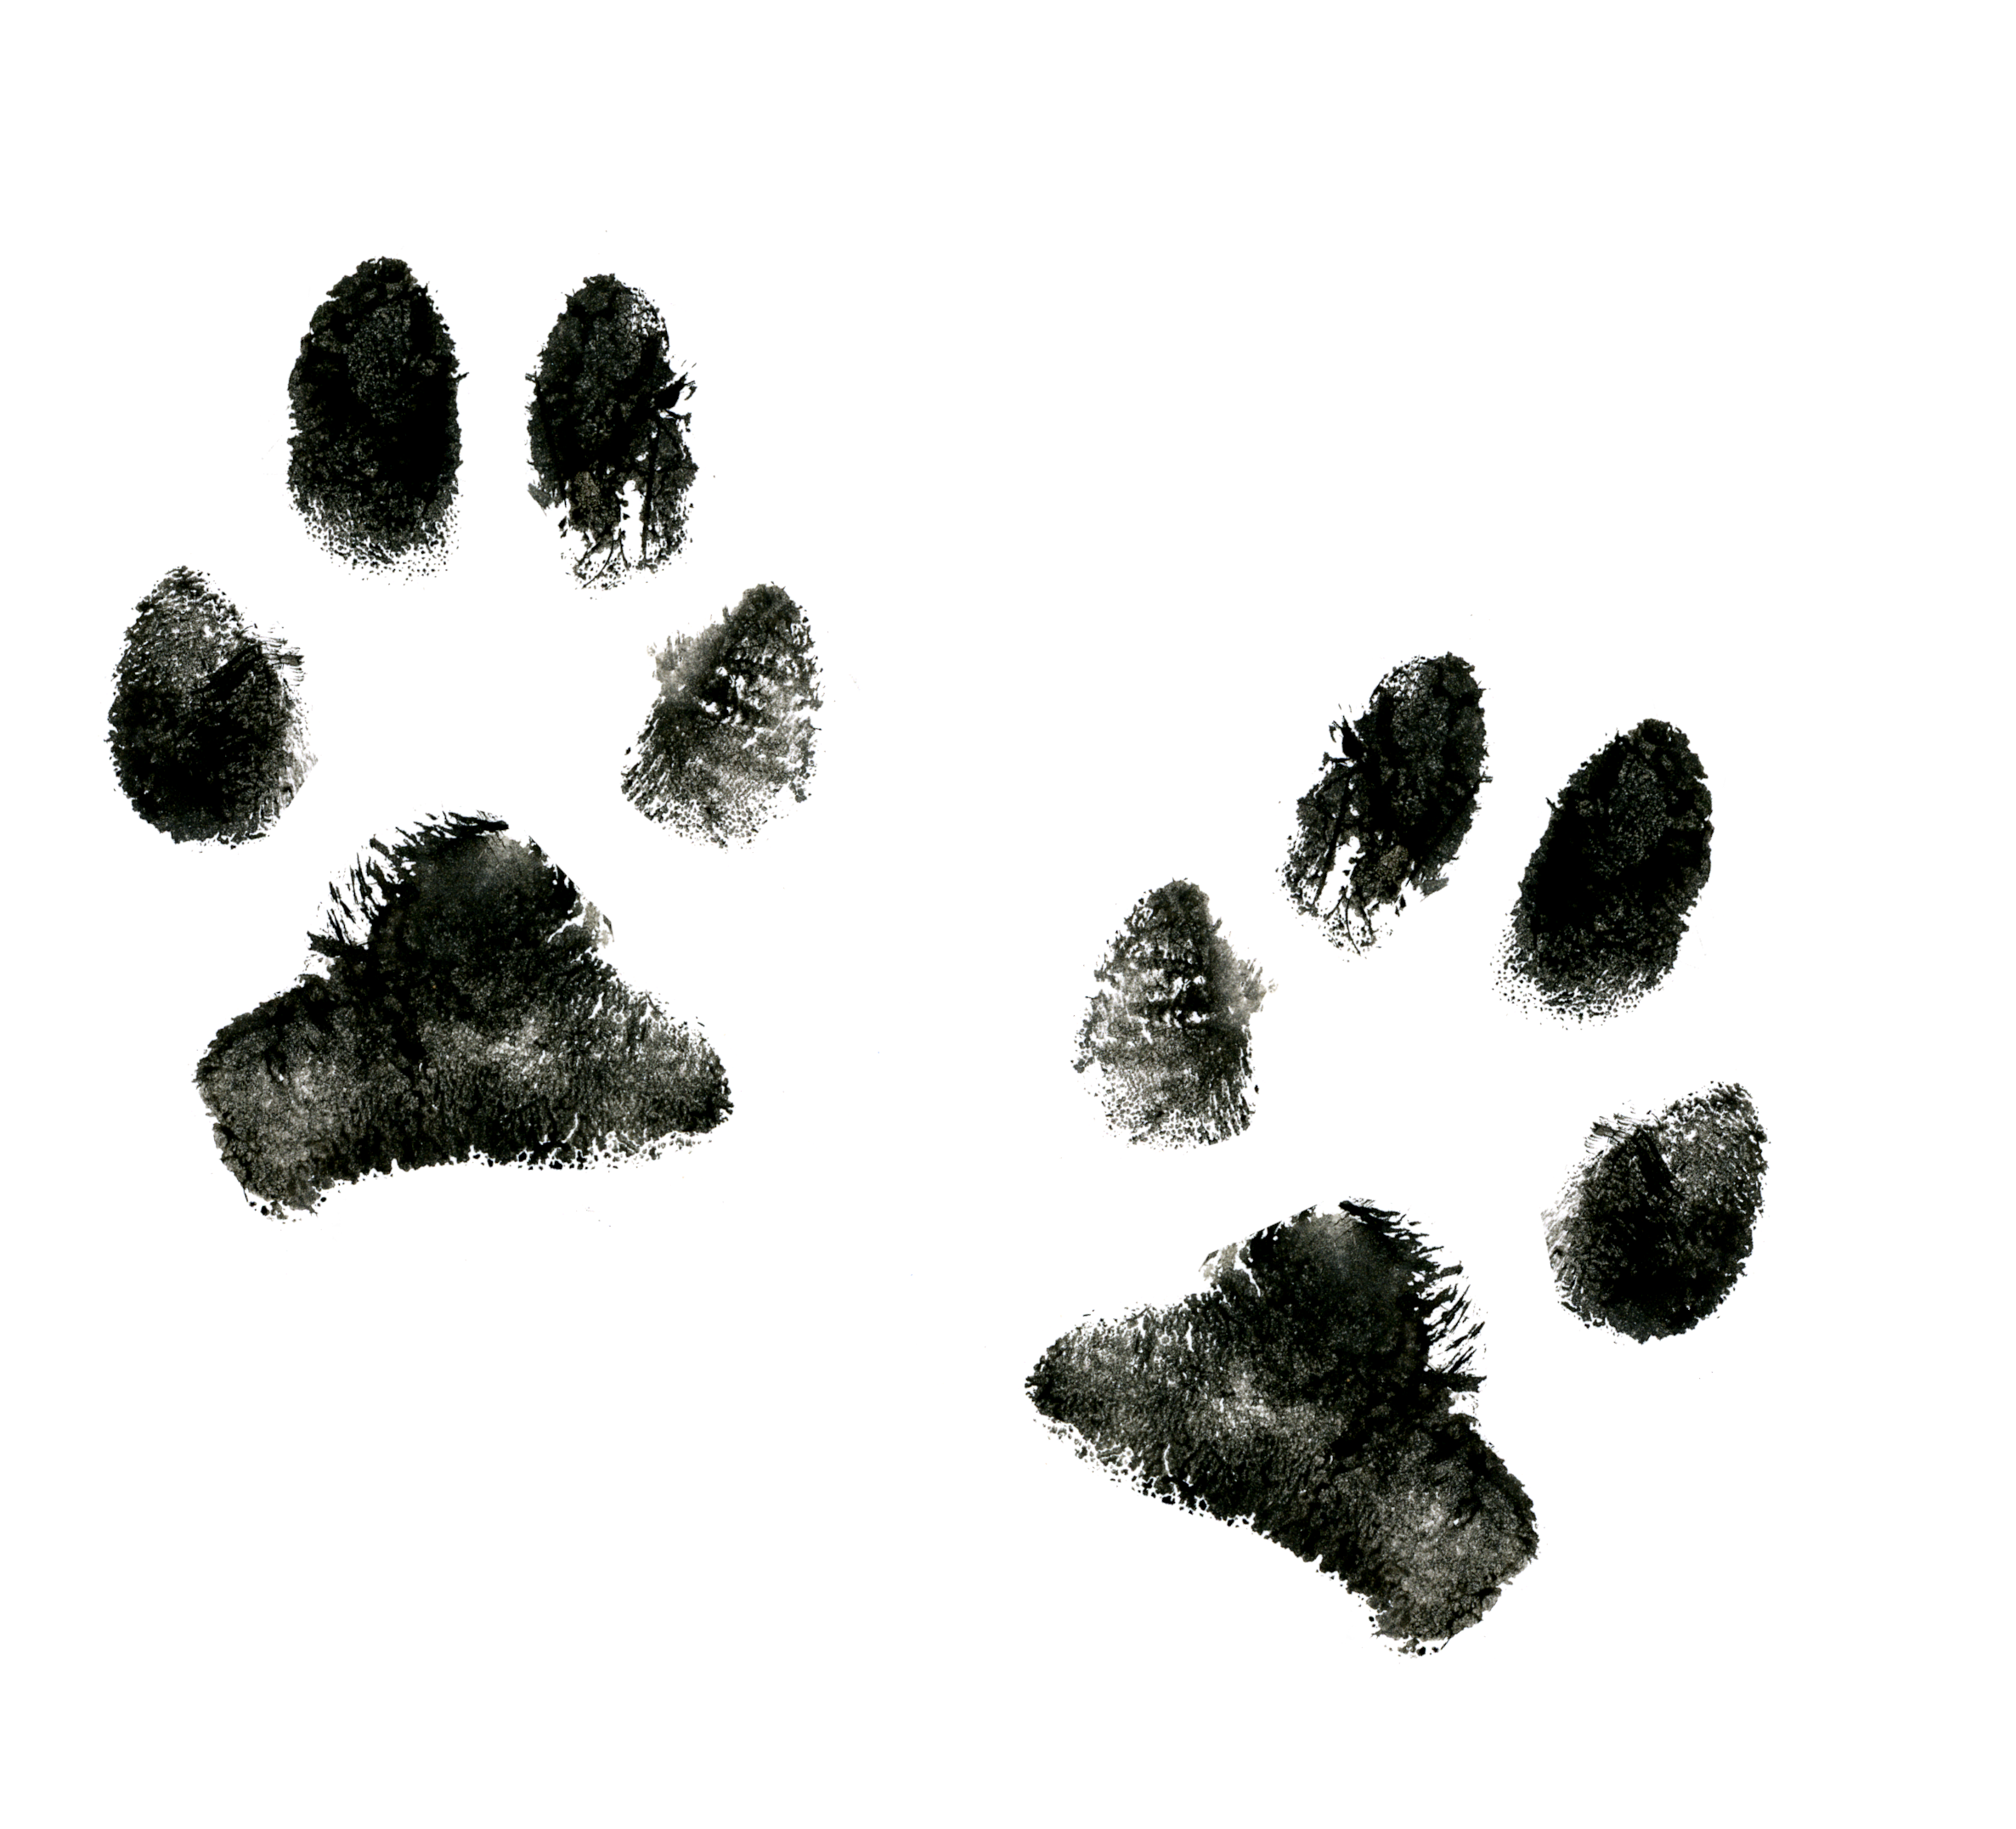
\includegraphics[width=1.7cm]{assets/2zpaw.png}
    \vfill
  \end{center}
}

\hyphenation{
\AuthorFirst
\AuthorLast
\Title
\Subtitle
}


\begin{document}
  \frontmatter

  \thispagestyle{empty}
  \null
  \vfill
  \begin{flushright}
    \DisplayFont Nevi'im
  \end{flushright}
  \vfill
  \cleardoublepage

  \pagestyle{plain}

  \doublespacing

  \begin{flushright}
    \null
    \vfill
    {\Huge\DisplayFont Nevi'im}

    {\DisplayFont Post-Self book III}

    \vfill

    {\Large\DisplayFont Madison Scott-Clary}
  \end{flushright}
  \thispagestyle{empty}

  \newpage

  \singlespacing
\thispagestyle{empty}
\begin{center}
    \noindent {\DisplayFont Also by Madison Scott-Clary}
    \TitleFamily

    \vspace{2ex}

    \emph{Arcana — A Tarot Anthology}, ed.

    \vspace{1ex}

    \emph{Rum and Coke — Three Short Stories from a Furry Convention}

    \vspace{1ex}

    \emph{Eigengrau — Poems 2015-2020}

    \vspace{1ex}

    \emph{ally}

    \vspace{2ex}
    
    \textbf{Post-Self}

    I. \emph{Qoheleth}

    II. \emph{Toledot}

    III. \emph{Nevi'im}

    IV. \emph{Mitzvot}

    \vspace{2ex}

    \textbf{Sawtooth}

    \emph{Restless Town}

    \emph{A Wildness of the Heart}

    \vspace{2em}

    Learn more at \emph{makyo.ink/publications}
\end{center}
\vfill
\singlespacing
{\small\parindent0pt\parskip5pt
\noindent Copyright \copyright\ 2020, Madison Scott-Clary. This work is licensed under the Creative Commons Attribution 4.0 International License. To view a copy of this license, visit \mbox{\emph{creativecommons.org/licenses/by/4.0/}} or send a letter to Creative Commons, PO Box 1866, Mountain View, CA

\vspace{1ex}

ISBN: \ISBN

\vspace{1ex}

\textit{Nevi'im}

\vspace{1ex}

Cover \copyright\ Iris Jay, 2022 --- irisjay.net

\vspace{1ex}

%\textit{This digital edition has been posted to Internet Archive and OpenLibrary by the author.}

\Edition\ Edition, \Year. All rights reserved.

\vspace{1ex}

This book uses the fonts Gentium Book Basic, {\DisplayFont Gotu} and {\TitleFont Linux Biolinum O} and was typeset with {\usefont{OT1}{cmr}{m}{n}\XeLaTeX}.

%Printed in the United States of America\\
%\EditionsList
}%\parindent0pt

\clearpage


  %\tableofcontents*
  \newpage
  \null
  \cleardoublepage

  %\onehalfspacing
  %\doublespacing

  % \null

\vfill

\noindent \textbf{Content Warning:} These stories contain descriptions of sex and sexuality. \emph{How Many} contains explicit description of mental health issues. \emph{Again} contains drug use.


  \mainmatter

  \pagestyle{ourbook}

  \cleardoublepage
  \null
  \thispagestyle{empty}
  \vfill
  \begin{quote}
    \small
    \emph{If you race only with foot-runners and they exhaust you, how then can you compete with horses? If you are secure only in a tranquil land, how will you fare in the jungle of the Jordan?}

    --- Jeremiah 12:5
  \end{quote}
  \vfill

  \part*{Prologue}
  Upon looking at the sky, many saw the stars and supposed that they must be the campfires of others. How far away they must be, to be such small points of light! Mere pinpricks in the black fabric of the night. They looked up, saw the campfires, and considered that they themselves might be just as the others were, looking out into the night and considering their own fire with dreaming minds.

  \vskip1em

  From \emph{An Expanded Mythology of our World} by

  May Then My Name Die With Me of the Ode clade
  \vfill

  \hypertarget{rj-brewster-2114}{%
\chapter{RJ Brewster — 2114}\label{rj-brewster-2114}}

There was some draw, some appeal to Dr.~Ramirez for RJ. At first, ey suspected that it was the quiet intensity of her confidence, the way she moved through the world with a hunger for knowledge that was at all times colored by the light of the desire to do right by the world as a whole. Then, ey thought that it might simply be that she was a good person. She was the one who believed hard enough and strong enough to follow up on the lost. She was the one who had actually tried, had actually moved forward at a pace that meant progress on the case. Recently, ey had been thinking that it was something more abstract than that.

Concrete? Abstract? The line had long since blurred to meaninglessness.

Ey had been lost for something beyond an eternity, for `eternity' implied the existence of time, or at least a form of time that actually meant something. Ey had been lost for a day longer than forever, and had ey been lost for only hours, as Sasha had, it would have been longer still. Even then, the word `longer' held far too much savor. It burned in the sinuses and left eir eyes stinging with tears.

She had been the first one in more than forever that ey had seen. She had been the one who broke through the wall of eir solipsistic existence and encouraged em to reengage with the world. As the orbits of eir life grew smaller and smaller, they had collapsed into a wandering figure-eight around Sasha, the one who made em complete, and Carter, the one who tied em to reality.

And so it was that, even beyond the meetings and interviews, beyond the panels and studies, ey found emself staying in touch with her. Once a week or two, ey would make the long walk from eir flat down to the cluster of UCL buildings and wait until she was free for lunch or dinner, or, had ey yet again forgotten the meaning of time, wait for her to arrive at work early in the morning so that they could grab coffee together.

She had not questioned it at all. Even that first time, after ey had hunted down her office in the UCL directory and arrived, unannounced, outside of it to wait awkwardly until she pulled back from her rig. She had simply smiled, shaken eir hand, and they had gone out for an afternoon cup of coffee with no further discussion. It had simply become the thing that they did every now and then.

Perhaps that was why ey liked her? Maybe.

Today, at lunch, ey joined Carter and two of her coworkers, Prakash Das and Avery Wilkins. Vietnamese had been the order of the day, and each of them had consoled em in turn about the loss of eir dear Priscilla, the cat who had been the only other grounding factor in eir life these last two years. A sudden loss of appetite, and then a sudden loss of life, and now ey needed the comfort of friends — or whatever it was that Carter had become — and some noise other than quiet jazz and London streets.

To their condolences, ey had simply raised eir cup of tea and nodded to them, saying, ``To deny the end is to deny all beginnings.''

``Delphic, as ever,'' Prakash said, though his smile and the lift of his own glass took any sting out of the words.

Ey smiled too, though ey could feel exhaustion tugging at eir cheeks. Ey had slept, ey knew, but did not remember when. ``Oh, trust me, there is plenty more where that came from.''

``Where \emph{does} it come from?'' Carter asked.

``I am not sure.'' Ey sipped at eir tea, still too hot to drink comfortably. ``Whatever wellspring that was unstoppered in\ldots in there.''

``And it's stuck around?''

Ey nodded.

``Think you'll ever turn it into something?'' Avery grinned to em. ``You know, write a book. Something like that.''

``I had not thought of that. I do not know that I could make a plot out of what feels like millions of words in a rock tumbler. Perhaps a poem.''

``Even infinite monkeys,'' Carter said, as she always did whenever the topic came up. ``Either way, you look thrashed, RJ. You sleeping okay?''

``No.~Maybe. I do not know.''

Perhaps sensing some emotion deeper than exhaustion laying beneath the equivocation, the table fell silent, and ey once again looked out the window into the greying afternoon, thumb-tip tapping rhythmically along each of the contacts on the middle joints of eir fingers.

Once the food arrived, the mood loosened up, and ey was able to smile and laugh and take part in the conversation, and even managed to apologize for being a damper on it only twice.

Spring rolls and phở occupied their attention for a while, then, and they ate in silence except for the occasional `good soup' and other such nothing compliments.

The time neared one o'clock, whatever that meant, and they settled up the bill and took the remainder of their conversation outside, hands stuffed in pockets while clouds of steam preceded them.

More laughter, more companionship. More warmth, despite the cold.

\emph{Perhaps this is why,} ey thought. \emph{Perhaps Carter and all of those she has introduced to me can add at least a little bit of warmth into the winter of my life.}

No, no, must not think such things. Ey had made eir decision, had ey not?

At the door to the building where the three worked, they all exchanged hugs, another bright spark of warmth in the cold afternoon, enough to carry em back home. Empty home, where ey could listen to more jazz and the distinct lack of purring. Empty home where ey could stare at eir rig and dare emself to delve in, if only to see if Sasha was about after work. Before work? What time was it for her? Time had left em; ey had only words.

Perhaps sleep.

Ey made it a block away before ey heard the sound of jogging behind em, and stepped over closer to the wall to let the jogger pass. The sound slowed, however, and ey was greeted once more by Prakash.

``Hey RJ, mind if I walk with you for a bit?''

``Sure.'' Ey frowned. ``Why? Do you not have work?''

He shrugged. ``I do, but I'm getting sick of being cooped up. Begged an additional hour off to just get out for a bit.''

``Alright.''

A silence stretched for a few minutes before Prakash said, ``Nice day, isn't it?''

``No,'' ey said, laughing. ``It is cold and gray. My cat is dead, my job is gone, and my two friends are someone I can only meet in a place I am terrified to go and a researcher of something that is no longer a problem.'' \emph{Memory is a mirror of hammered silver,} the litany continued within as always. Ey hoped silently. \emph{A weapon against the waking world.} ``Dreams are the plate-glass atop memory: a clarifying agent against the sun. Sorry.''

Prakash nodded, as though this was part of a normal conversation. ``You're okay, RJ. No luck on the job front? Are you doing alright for cash?''

Ey rubbed away unwelcome tears and nodded. ``Enough for another six months here, and then I need to either find a new job or move back to America. My parents have said--''

``Would you be interested in a job offer?''

``From the university?''

He shook his head. ``No.''

``Where then? I did not know you worked anywhere else.''

``Work is probably the wrong word, here,'' Prakash said, grinning. ``But, I mean, if you don't mind heading out of the WF for a while, I might have something for you.''

Part of RJ stopped up short — though not, ey noted dispassionately, eir body — and ey blinked rapidly down towards the ground. This was a new, strangely shaped bit of information. There was no opening within eir mind that would fit it perfectly, so ey carefully set it aside. \emph{The waking world fogs the view and time makes prey of remembering.} ``And what would this job that you do not work at entail? I am wary of sims.''

``Of course. Minimal work on the 'net.'' He seemed to consider for a moment, then shrugged. ``Well, no work on the 'net, actually, but minimal work in-sim.''

Ey nodded, waited for Prakash to continue.

``Carter was kind enough to provide us with some extra information. Michelle's core dump from when she got lost, yours from the theater sim that the techs were careless enough to leave around. Some people I'm\ldots not working with at my non-job with have been digging through those and, in combination with the testimonies of the lost, come up with some interesting hypothes--''

``A way back?''

The intensity with which ey replied startled the researcher, who held up his hands defensively. ``Sorry, RJ. If I overstepped--''

``No, sorry,'' ey said. ``I did not mean to shout. If it is a way back, I will say yes. If it is a way to `fix' whatever I have become, I will say no and do not wish to waste your time.''

Prakash relaxed and shook his head. ``I see. You've mentioned not wanting to lose what you have. I wouldn't have offered if that was on the table. They're not really thinking of a way back, no, but maybe a way forward. Use what you taught us to find — or make — somewhere new.''

At this, ey really did stop up short. ``What do you mean, `somewhere new'?''

``Arms races have fallen out of style. It's not really considered fashionable to stockpile weapons or anything anymore.''

RJ blinked, nonplussed.

``Technology, however, brings with it a status of its own.'' Prakash smiled, neither pityingly nor happily. Dreamily. ``So if, as you say, dreams are the plate-glass atop memory, and if, as you've said in the past, getting lost put you in a mirrored cage, then these are bits of information related to technology. If one could drop the cage metaphor and set up a mirrored \emph{world}, well, that would be quite the status symbol.''

RJ stood a while in thought, searching Prakash's face until the man averted his eyes, and even after. ``What would be required of me?''

``Nothing, for now. Just to stay in touch. Eventually, though, we'll get you somewhere we can dig into research and after that, you'll be one of the founders of something big. Really big.''

The words came in a torrent, then, and with such an intensity that ey staggered and had to clutch at Prakash's arm for support. ``The flow of prophecy climbs up through the years, winter upon winter upon winter, and compels the future to do its bidding. The prophet is only a pipe that sounds when the past\ldots shit. I am sorry. All of that to say `yes'. I am sorry.''

Once the shock of the onrush of words wore off, Prakash nodded, smiling cautiously. ``It's okay, RJ. Like I said, nothing needs to be done right now. And I trust that you know not to mention this to anyone. Someone else will talk to Michelle about it. Talk to each of the lost, I mean. No need to bring it up with them. When things are lined up, we can go for another walk after coffee or something. Sound good?

Ey swallowed dryly, nodded. ``Thank you. I will hold on until then.''

They started walking again, the researcher explaining that he really did need the air, since all that waited for him was an office sim.

RJ did not mind. What sadness that dug at em from Prisca's passing had been blunted, softened by the prospect of something new. Something ahead of em. Something to look forward to that did not bring with it more exhaustion, more words.

``You know,'' Prakash said thoughtfully. ``I know the things you say sometimes aren't really intentional or anything, but you're not wrong.''

``Mm?''

``About prophecy, I mean. Just over two years since you got back and here you are, being invited to compel the future to do your bidding using what you learned.''

Ey laughed, earnest and true. ``I suppose so. I was going to say''the prophet is only a pipe that sounds when the past demands it'', and given that I cannot seem to live in this world anymore, that demand is getting to be overwhelming.''


  \part{Anticipation}
  They dreamed and thought and considered, and then many of those who knew the ways to navigate the seas argued that reaching one of those campfires would be a way to quell the loneliness that they felt as a hole in their hearts. ``Perhaps they will fill us with joy! And even if they fight against us or sow strife, is that not a form of companionship?''

  Others were more cautious about the venture, however. ``Is a danger not a danger?'' they said. ``Is a risk not a risk? We must also consider that we might ourselves be overcome by their might. Is it worth stoking that fire?''

  Still others spoke thoughtfully, ``It is a danger here, as well. There are wild animals in the dark, and there are those who might fight against us here. Perhaps the goal of exploration is also to ensure the security of ourselves! Could we not also use this as a chance to ensure that we live on?''

  \vskip1em

  From \emph{An Expanded Mythology of our World} by

  May Then My Name Die With Me of the Ode clade
  \vfill
  
  \hypertarget{true-name-2124}{%
\chapter{True Name—2124}\label{true-name-2124}}

The next meeting spot for the Council of Eight was in a rooftop bar. However, given that that rooftop bar was in the midst of a block of apartment buildings and vertical malls that had built with shared walls, such that there was a cubic half-mile of stair-climbing, elevator rides---down as well as up---and trestles that bridged buildings of lower height than higher ones, it was more adventure getting to the venue than the meeting itself promised.

Still, The Only Time I Know My True Name Is When I Dream climbed.

The apartment buildings ranged from serviceable to gutted, and more than one time, she had to step carefully through a path covered in rubble. She could not decipher whether this was due to abandoned renovations, some unknown battle, or the simple degradations of time.

The malls offered different dichotomies. Some of them were sparkling new with speakers that whispered to her in Mandarin and lights that shouted in her face, while others played placid muzak through halls lit only by emergency lights, darkened storefronts yawning onto scuffed and over-waxed parquet floors.

She wondered who it was that had owned this sim, what collective it was that had decided to mash all the best and worst multiple clashing centuries worth of Kowloon Walled City and the North American Central Corridor.

And then, the rooftop bar. Despite no vehicle entrance to the complex, this was situated on the top level of what appeared to be a car park straight out of a mid-western American airport, complete with one or two of those vehicles that seemed perpetually parked, ones that had lingered for months or years, accruing a parking debt of thousands, tens of thousands of dollars.

The bar itself was a pop-up affair, with walls and ceiling of corrugated plastic held together with rivets and tape, a bar-top that was a few two-by-eights set across a trestle, fronted with further corrugated plastic to keep the patrons from kicking fridges or sinks out of alignment.

The drinks: early 2100s hipster bullshit, all intensely sweet or riddled with smoke-scented fizzy water or long strips of seaweed or clams within the ice cubes, steadily making the drink more and more savory over time.

True Name found it all confusing and jarring.

She liked it immediately.

Debarre was already at one of the tables---similarly cobbled together---sipping something that seemed to be all foam. He waved to her as she entered, and she waved back, heading to the bar to pick up one of those seaweed concoctions before joining him.

``That looks fucking gross, Sasha.''

She laughed and shrugged. ``I am True Name, but yes, it really does. If we are going to meet in a place that gives me a headache to walk through, it is probably best that I get something with\ldots protein? Is that how this works?''

``Uh, sorry. Yeah. True Name.'' The weasel splayed his ears and averted his eyes. ``Can we talk about that sometime?''

``Yes, but probably as Michelle, if that is okay.''

``Why?''

``She is\ldots closer to it than I am.''

Debarre gripped his glass more tightly and twisted sideways to swing his leg over the bench and straddle it. ``Yeah, I don't get it. Before everyone else gets here, can you at least give me a sentence or two?''

``When she forked, when I\ldots became me, she decided not to fork that part of her that suffers if that is the right word.'' True Name frowned. ``Already we are drifting further apart. The species remains, the appearance and the speech patterns remain, the \emph{mind} remains, but not that part of her that is so split. I am me, I am templated off of Sasha, because being both Michelle and Sasha at the same time was no longer tolerable.''

He shrugged, still staring down into his drink. ``I can't speak to that, I guess. But why Aw--''

True Name slammed her glass down on the table a bit harder than intended, some of the drink spilling over her hand. ``Do not say that fucking name.''

The weasel jumped at the sudden intensity, and when he recovered, he finally met her gaze. His expression softened from fear and anger to a tired bleakness. That moment drew out for a long few seconds of quiet and seething sadness. He reached for a napkin from the dispenser at the end of the table and handed it to her. ``Here.''

She hesitated, mastered a surge of unnamed emotion, and accepted the napkin to wipe the sticky drink from her paw and then, on realizing that she was crying, the tears from her face. ``Sorry, I am just\ldots{}''

``We'll talk.'' He reached over and gave her dry paw a squeeze in his own. ``Michelle and I will. There's something I'm missing here is all, and I want to figure out why more than what.''

True Name hid her muzzle in her drink and pretended to take a sip until she was sure she wouldn't slur her words when she spoke. ``Thank you. She is open to messages still, I will let you two work it out. For now, I need to focus on the meeting. Jonas and Zeke are here.''

Looking over his shoulder, Debarre nodded and turned to sit on the bench to face her again, leaving room for the other two. Jonas settled next to True Name so that they could give their speech together when the time came, and Zeke, that shifting bundle of rags and grime slid onto the bench beside Debarre.

``Good afternoon,'' the almost-face within the bundle rasped.

Jonas grinned. ``It's morning, isn't it?''

A pseudopod that may have been a hand waved the comment away. ``Time has lost all meaning. I seem to have forgotten how to sleep, these days.''

``You need a vacation like Michelle.''

There was a low rattle from the rags, and True Name imagined that must be Zeke's laughter. ``Don't tempt me. I don't have the funds to fork, so you'd be down to seven.''

``Why \emph{did} you make it so expensive?'' Jonas elbowed True Name in the side.

She held up her paws defensively and laughed. ``I did not. The price is tied to system capacity.''

``The laws of physics were a mistake and reputation is a lie.''

``It is the best limiting factor that we have that is not a complete fabrication, at the moment.''

``I rather miss coins.''

``My dad used to collect coins, you know.''

And so on, until the table was full and the cone of silence fell.

``Sasha? Uh\ldots True Name. Jonas?'' one of the well-dressed triad asked.

``Right,'' Jonas said, setting his drink down. ``The bill. Things are progressing slowly, as they always do, but it sounds like they might start picking up steam shortly. Our main contact on the DDR side, one Yared Zerezghi based out of the Northeast African Coalition, says that some of the governments are starting to take interest in the bill, which could work to our advantage. Having it just be a direct vote would mean that we would have far, far more representatives to convince, since that'd mean essentially everyone on the DDR. The more governments in play, the more the role of the DDR shrinks.''

``How does that even begin to help? Aren't they super stodgy?'' Debarre asked.

``They can be,'' Jonas hedged. ``But if we can form contacts with each of them, we can argue our case directly. Yared might be the one to give us a good in for the NEAC, and I still have some Western Fed contacts.''

``Anyone for the S-R Bloc or anywhere in SEAPAC? Middle east? India?''

The trio of suits raised their hands. ``S-R Bloc. We don't know any of the oligarchs directly, but we had some big money interests of our own.''

``Israel,'' Zeke said, then laughed at the awkward silence that followed. The trio frowned. ``Sorry, nothing to be done there.''

``And SEAPAC?''

user11824 shrugged. ``I was a nobody, but I was a Maori nobody.''

``You had enough to upload. That has to count for something, doesn't it?''

He shrugged again.

``We will take all the help we can get,'' True Name said. ``Even from nobodies.''

``Alright, I'll poke mom.''

Zeke nodded to True Name. ``What's your take on the situation?''

She stirred her drink to buy herself some time to think. ``I think it is leaning our way. One of the big arguments remains speciation, but Yared's turning that into a pro-rights argument instead of a neutral- or anti-rights one. His voice is getting louder, too. It sounds like he is getting a lot more upvotes on his posts than before.''

``That's good.''

True Name nodded. ``I think so. He is not the biggest voice on the issue yet, but it sounds like he is probably in the top three.''

``You said he's NEAC, right?''

``Yeah, Addis Ababa,'' Jonas said. ``Not exactly the seat of power, but I guess not everything has to be Cairo. Sounds like we have a good mix, at least. No one from South America?''

Everyone shook their heads.

``I suppose that's alright. They're a big enough voice in Western Fed, but they're still in the shadow government side of things. They don't even have the shadow minister of System affairs.''

``Who does?''

``Lithuania.''

One of the suits laughed, and Debarre looked blank.

``Politics,'' Jonas said, grinning lopsidedly.

``If you say so.''

After a moment's silence, Zeke rasped, ``So what are our next steps?''

``Let's all talk to our respective interests---Zeke too---and we'll meet again soon. True Name and I will keep working with Yared and guide as best we can from our side. Speaking of, though, any thoughts on the speciation topic?''

Six sets of eyes flitted between Debarre and True Name, between weasel and skunk, then the whole council laughed.

``I don't give a shit,'' user11824 said. ``But if your Yared guy can twist that argument against the opposition, then that's just one more tool, isn't it?''

``We aren't seeing that,'' the man in the suit spoke up. ``Two thirds of our power structure still think child restrictions are a good enough idea that those laws have bled into Russia. I'm pretty sure they see speciation as a positive. What better way to help in population control?''

One of his companions shrugged, ``I wouldn't be surprised if they started putting limitations on uploading by gender, but that is a separate topic.''

``Zeke?''

The pile of rags shifted in a shrug.

``Debarre? True Name? Anything you can leverage?''

The weasel laughed. ``I mean, if you want to point to us as an example to push that along, and Yared's tack seems to be working, go for it.''

``Alright. It's something you can suggest to your respective interests if you think it'll help. We'll reevaluate next meeting. Anything else on the agenda?''

Everyone shook their heads, then lifted their glasses to a toast. The cone of silence dropped.

``Well, then, you are all free to stick around or go if you want,'' True Name said. ``I am going to stay and get well and truly plastered.''

  \hypertarget{true-name-2124}{%
\chapter{True Name—2124}\label{true-name-2124}}

The next meeting spot for the Council of Eight was in a rooftop bar. However, given that that rooftop bar was in the midst of a block of apartment buildings and vertical malls that had built with shared walls, such that there was a cubic half-mile of stair-climbing, elevator rides---down as well as up---and trestles that bridged buildings of lower height than higher ones, it was more adventure getting to the venue than the meeting itself promised.

Still, The Only Time I Know My True Name Is When I Dream climbed.

The apartment buildings ranged from serviceable to gutted, and more than one time, she had to step carefully through a path covered in rubble. She could not decipher whether this was due to abandoned renovations, some unknown battle, or the simple degradations of time.

The malls offered different dichotomies. Some of them were sparkling new with speakers that whispered to her in Mandarin and lights that shouted in her face, while others played placid muzak through halls lit only by emergency lights, darkened storefronts yawning onto scuffed and over-waxed parquet floors.

She wondered who it was that had owned this sim, what collective it was that had decided to mash all the best and worst multiple clashing centuries worth of Kowloon Walled City and the North American Central Corridor.

And then, the rooftop bar. Despite no vehicle entrance to the complex, this was situated on the top level of what appeared to be a car park straight out of a mid-western American airport, complete with one or two of those vehicles that seemed perpetually parked, ones that had lingered for months or years, accruing a parking debt of thousands, tens of thousands of dollars.

The bar itself was a pop-up affair, with walls and ceiling of corrugated plastic held together with rivets and tape, a bar-top that was a few two-by-eights set across a trestle, fronted with further corrugated plastic to keep the patrons from kicking fridges or sinks out of alignment.

The drinks: early 2100s hipster bullshit, all intensely sweet or riddled with smoke-scented fizzy water or long strips of seaweed or clams within the ice cubes, steadily making the drink more and more savory over time.

True Name found it all confusing and jarring.

She liked it immediately.

Debarre was already at one of the tables---similarly cobbled together---sipping something that seemed to be all foam. He waved to her as she entered, and she waved back, heading to the bar to pick up one of those seaweed concoctions before joining him.

``That looks fucking gross, Sasha.''

She laughed and shrugged. ``I am True Name, but yes, it really does. If we are going to meet in a place that gives me a headache to walk through, it is probably best that I get something with\ldots protein? Is that how this works?''

``Uh, sorry. Yeah. True Name.'' The weasel splayed his ears and averted his eyes. ``Can we talk about that sometime?''

``Yes, but probably as Michelle, if that is okay.''

``Why?''

``She is\ldots closer to it than I am.''

Debarre gripped his glass more tightly and twisted sideways to swing his leg over the bench and straddle it. ``Yeah, I don't get it. Before everyone else gets here, can you at least give me a sentence or two?''

``When she forked, when I\ldots became me, she decided not to fork that part of her that suffers if that is the right word.'' True Name frowned. ``Already we are drifting further apart. The species remains, the appearance and the speech patterns remain, the \emph{mind} remains, but not that part of her that is so split. I am me, I am templated off of Sasha, because being both Michelle and Sasha at the same time was no longer tolerable.''

He shrugged, still staring down into his drink. ``I can't speak to that, I guess. But why Aw--''

True Name slammed her glass down on the table a bit harder than intended, some of the drink spilling over her hand. ``Do not say that fucking name.''

The weasel jumped at the sudden intensity, and when he recovered, he finally met her gaze. His expression softened from fear and anger to a tired bleakness. That moment drew out for a long few seconds of quiet and seething sadness. He reached for a napkin from the dispenser at the end of the table and handed it to her. ``Here.''

She hesitated, mastered a surge of unnamed emotion, and accepted the napkin to wipe the sticky drink from her paw and then, on realizing that she was crying, the tears from her face. ``Sorry, I am just\ldots{}''

``We'll talk.'' He reached over and gave her dry paw a squeeze in his own. ``Michelle and I will. There's something I'm missing here is all, and I want to figure out why more than what.''

True Name hid her muzzle in her drink and pretended to take a sip until she was sure she wouldn't slur her words when she spoke. ``Thank you. She is open to messages still, I will let you two work it out. For now, I need to focus on the meeting. Jonas and Zeke are here.''

Looking over his shoulder, Debarre nodded and turned to sit on the bench to face her again, leaving room for the other two. Jonas settled next to True Name so that they could give their speech together when the time came, and Zeke, that shifting bundle of rags and grime slid onto the bench beside Debarre.

``Good afternoon,'' the almost-face within the bundle rasped.

Jonas grinned. ``It's morning, isn't it?''

A pseudopod that may have been a hand waved the comment away. ``Time has lost all meaning. I seem to have forgotten how to sleep, these days.''

``You need a vacation like Michelle.''

There was a low rattle from the rags, and True Name imagined that must be Zeke's laughter. ``Don't tempt me. I don't have the funds to fork, so you'd be down to seven.''

``Why \emph{did} you make it so expensive?'' Jonas elbowed True Name in the side.

She held up her paws defensively and laughed. ``I did not. The price is tied to system capacity.''

``The laws of physics were a mistake and reputation is a lie.''

``It is the best limiting factor that we have that is not a complete fabrication, at the moment.''

``I rather miss coins.''

``My dad used to collect coins, you know.''

And so on, until the table was full and the cone of silence fell.

``Sasha? Uh\ldots True Name. Jonas?'' one of the well-dressed triad asked.

``Right,'' Jonas said, setting his drink down. ``The bill. Things are progressing slowly, as they always do, but it sounds like they might start picking up steam shortly. Our main contact on the DDR side, one Yared Zerezghi based out of the Northeast African Coalition, says that some of the governments are starting to take interest in the bill, which could work to our advantage. Having it just be a direct vote would mean that we would have far, far more representatives to convince, since that'd mean essentially everyone on the DDR. The more governments in play, the more the role of the DDR shrinks.''

``How does that even begin to help? Aren't they super stodgy?'' Debarre asked.

``They can be,'' Jonas hedged. ``But if we can form contacts with each of them, we can argue our case directly. Yared might be the one to give us a good in for the NEAC, and I still have some Western Fed contacts.''

``Anyone for the S-R Bloc or anywhere in SEAPAC? Middle east? India?''

The trio of suits raised their hands. ``S-R Bloc. We don't know any of the oligarchs directly, but we had some big money interests of our own.''

``Israel,'' Zeke said, then laughed at the awkward silence that followed. The trio frowned. ``Sorry, nothing to be done there.''

``And SEAPAC?''

user11824 shrugged. ``I was a nobody, but I was a Maori nobody.''

``You had enough to upload. That has to count for something, doesn't it?''

He shrugged again.

``We will take all the help we can get,'' True Name said. ``Even from nobodies.''

``Alright, I'll poke mom.''

Zeke nodded to True Name. ``What's your take on the situation?''

She stirred her drink to buy herself some time to think. ``I think it is leaning our way. One of the big arguments remains speciation, but Yared's turning that into a pro-rights argument instead of a neutral- or anti-rights one. His voice is getting louder, too. It sounds like he is getting a lot more upvotes on his posts than before.''

``That's good.''

True Name nodded. ``I think so. He is not the biggest voice on the issue yet, but it sounds like he is probably in the top three.''

``You said he's NEAC, right?''

``Yeah, Addis Ababa,'' Jonas said. ``Not exactly the seat of power, but I guess not everything has to be Cairo. Sounds like we have a good mix, at least. No one from South America?''

Everyone shook their heads.

``I suppose that's alright. They're a big enough voice in Western Fed, but they're still in the shadow government side of things. They don't even have the shadow minister of System affairs.''

``Who does?''

``Lithuania.''

One of the suits laughed, and Debarre looked blank.

``Politics,'' Jonas said, grinning lopsidedly.

``If you say so.''

After a moment's silence, Zeke rasped, ``So what are our next steps?''

``Let's all talk to our respective interests---Zeke too---and we'll meet again soon. True Name and I will keep working with Yared and guide as best we can from our side. Speaking of, though, any thoughts on the speciation topic?''

Six sets of eyes flitted between Debarre and True Name, between weasel and skunk, then the whole council laughed.

``I don't give a shit,'' user11824 said. ``But if your Yared guy can twist that argument against the opposition, then that's just one more tool, isn't it?''

``We aren't seeing that,'' the man in the suit spoke up. ``Two thirds of our power structure still think child restrictions are a good enough idea that those laws have bled into Russia. I'm pretty sure they see speciation as a positive. What better way to help in population control?''

One of his companions shrugged, ``I wouldn't be surprised if they started putting limitations on uploading by gender, but that is a separate topic.''

``Zeke?''

The pile of rags shifted in a shrug.

``Debarre? True Name? Anything you can leverage?''

The weasel laughed. ``I mean, if you want to point to us as an example to push that along, and Yared's tack seems to be working, go for it.''

``Alright. It's something you can suggest to your respective interests if you think it'll help. We'll reevaluate next meeting. Anything else on the agenda?''

Everyone shook their heads, then lifted their glasses to a toast. The cone of silence dropped.

``Well, then, you are all free to stick around or go if you want,'' True Name said. ``I am going to stay and get well and truly plastered.''

  \hypertarget{codrin-bux103lan-2346}{%
\chapter{Codrin Bălan — 2346}\label{codrin-bux103lan-2346}}

It took both both eir partners to talk Codrin down from eir desire to simply get right to work.

\emph{``My dear, if, as he said, Tycho was going to take a nap, perhaps you ought to do the same.''}

``I know,'' ey replied, shoulders sagging. ``It's hard to get out of that mindset of having to just work.''

``I know it's enjoyable,'' the fox's partner said. ``But seriously, Codrin, even if you're not going to take a nap, take a thermos out onto the prairie and walk for a bit. Tycho is going to need quite a bit of help, given what you told us of him--''

\emph{``And if True Name is already involved.''}

``That too, yeah. So it's probably best to go into the whole thing prepared for jittery astronomers and\ldots well, whatever True Name is, these days.''

Codrin nodded. ``That makes sense, at least. Do we even have a thermos?''

``Probably. I'll go digging. Might as well make a fresh pot, while I'm up.''

\emph{``You, my love, are a true delight,''} Dear said, tail flitting this way and that.

They grinned, walked off to the kitchen, and started clattering around in cupboards for a coffee therm.

``Dear, have you talked to True Name recently?'' Codrin asked after a polite pause.

It shook its head. \emph{``Not in terms of a conversation, at least. I have received a few messages from her in the intervening years, several of which were sent to several Odists as a group.''}

``She does that? What are they? Orders or something?''

It shook its head, ears flapping slightly at the movement. \emph{``No.~Or, well, not exactly. They are simply updates, or replies to other, ongoing conversations. Many of us still communicate with each other on a somewhat regular basis, and I have been looped into several of those conversations over the years.''}

``Wait,''not exactly``?''

\emph{``You have met her. She does not need to order, oftentimes. She simply suggests.''}

Ey frowned. ``I sometimes worry that we've been attributing almost magical manipulative abilities to her, honestly.''

Dear shrugged. \emph{``Perhaps, but she also has had more than two hundred years of study under her belt to find all of the best ways to interact with people. May Then My Name was something of a let-down for her, I think, even from the very beginning, so she had to learn to take on that mantle herself.''}

``Especially over the last few years, you mean? With Ioan?''

\emph{``Perhaps, though I think that might be ancillary to the fact that our dear May is not on the LVs at all.''}

Ey blinked, laughed. ``Okay, well, fair. I'd almost forgot.''

The fox gave em a strange look. \emph{``You forgot that May Then My Name was not here?''}

Their partner showed up, a cup of coffee in one hand and a (far too large) thermos in the other. ``Are you forgetting things again, Codrin?''

``No, no,'' ey said, accepting the thermos with a frown. ``Or, well, kind of. I didn't forget that May Then My Name wasn't here, just the ramifications of that, that True Name might not have her as a tool.''

\emph{``That is more understandable, yes,''} the fox said. \emph{``Perhaps the True Name here on Castor has diverged from that on the L5 System in that respect, perhaps not. I suspect that both are disappointed, in their own ways.''}

Codrin fiddled with the thermos, ensuring that the lid was a mug when removed — two nested ones, actually — then nodded, standing. ``I don't know how many dimensions she's thinking on, but I also wouldn't be surprised if she had a cost-benefit analysis on losing her to Ioan.''

\emph{``I would not be surprised, no, which would mean that she has planned around that eventuality. I am sure that May Then My Name is keeping an eye on that. Do not let us keep you, though, my dear. Go for your walk. Think about something else. Enjoy the cold, build a cairn around your worries, and then return safe.''}

Ey smiled, leaned down to kiss the fox between the ears, then eir other partner on the cheek. ``I didn't know that was possible, but I'll try. Back in a bit.''

Ey made it two cairns out before caving to the desire to simply get started, and stepped over to Tycho's field. There was a ping of amusement from Dear, to which ey replied with a guilty apology and an acknowledgement that ey'd return soon, all while waiting for eir eyes to adjust to the sudden darkness.

The next sensorium message was a gentle ping to Tycho — nothing so loaded with anxiety as the one ey'd received this morning, just an acknowledgement, a view of the stars.

A voice came from somewhere behind em. ``Codrin?''

Ey whirled around to see a dim cone of red light shining on the ground, illuminating feet in a pair of well-worn boots. ``Tycho? Sorry for intruding like this. I hope I'm not waking you or anything.''

``No, no. Come in. I haven't been able to sleep since True Name left.''

There was a small click and then a ray of further red light spread out from a doorway, showing a small hut nestled within the trees. Ey let emself be guided into the door, finding a sparsely decorated room — a desk, a bed, and a massive cork board nailed to the wall, covered in at least three overlapping layers of notes.

``Thanks for having me,'' ey said, sitting on the offered chair while Tycho claimed the edge of the bed. Once the door was shut, a switch shifted the red light to a normal, warm desk lamp. ``I should've mentioned that I'd be coming over, first.''

He waved away the apology. ``I knew you'd be here, though I didn't know when.''

Codrin paused in the middle of unscrewing the lid to the thermos. ``You knew?''

``True Name said you would.''

Ey frowned, finishing opening the thermos and offering Tycho one of the two mugs of coffee. ``What did she say about me?''

``She didn't talk with you?''

Ey shook eir head. ``Did she say she would?''

Tycho sipped at the coffee, winced, and set the mug aside to cool. ``No, she just talked as though she had, or at least that she knew you'd be working with me.''

``Of course she did,'' ey murmured. ``She knows me too well.''

The astronomer ground the heels of his palms against his eyes. ``I feel like she knew me too well, too. We had what felt like a wonderful conversation where she offered me a job, asked me to fork to send an instance with her to keep working with her, but then quoted some bit of poetry at me and I couldn't tell if it was a death threat or a warning or whatever. I'm still trying to recover from that.''

``I'm guessing you said yes to both the job offer and the fork?''

He nodded. ``It all just sounded so normal. There didn't seem like anything else to do.''

``Can you tell me more about both?''

``Well, she said that she a good deal about the communications and that she'd like me to come help her with the mechanics of that. She'd help me out with resources and I'd teach her about Artemis as I learned it.''

``Artemis? Is that what they're calling the remote\ldots ship? Vehicle?''

He nodded. ``Vehicle, I think. She said they're calling it Artemis, that I should tag my fork \#Artemis, and that those on the ship were either Artemisians or Sea People, which I didn't get.''

Codrin leaned back in the seat, thinking. ``Sea People might be a reference to something from the Mythology, or it could be a reference to a theory about a marauding group of seafarers during the Bronze Age collapse. There was a bunch of talk about how this group had sacked much of the ancient near east and northern Africa, leading to the prolongation of the collapse.''

Tycho's eyes grew wide. ``Do you think that's what she's getting at with the reference? That these are going to be some marauders coming to mess with the LV?''

Ey shrugged. ``Who knows. Probably both, honestly. Maybe there's even some reference that we're missing. She's True Name, there really is no way of telling.''

Nodding, Tycho scooted back on the bed until his back was to the wall, then brought his knees up to his chest. He looked small to Codrin, somehow diminished after the events of the last\ldots goodness, had it only been a day? Diminished, yes, and younger, though he'd always looked as though he was not yet out of his forties in his well-groomed salt-and-pepper hair and well-kept beard.

They sat in silence for a while. Codrin could not guess what the astronomer was thinking about, though ey could see his eyes occasionally darting this way and that, as though connecting one idea to another in the air as well as in his head.

On eir part, ey began structuring the project. There would have to be the journalistic aspect of it, much closer to that of the Qoheleth project than the History, but if the conservative Odists were also involved, there'd likely also be far more observing than researching.

``Tycho,'' ey said, startling him out of a reverie. ``Do you know what an amanuensis is?''

``Like a recorder? Someone who takes notes?''

``Well, in part, but also someone who thinks about what they're writing,'' ey said, tapping at eir temple. ``They aren't a scribe or a court recorder, but someone there to witness and digest a conversation.''

``Like a clerk?'' He grinned. ``We used to have one of those for our club, who would take minutes of the meetings and such.''

Ey nodded. ``Certainly closer to that than a recorder, yeah. I bring this up because that will be my job in all of this, but I think it'll also be yours. Things like the History are all well and good, and I loved putting the work into it, but I also really enjoy doing this. I may wish that the things I get caught up in weren't always so dramatic, but I'll take what I can get.''

``What do you mean, it'll be my job too?'' he asked.

``Just that you will also be witnessing and thinking about this project, and then coming up with ideas related to it to be compiled into a coherent understanding. That's why we'll be working together, I think. I'm trained to do this work in particular, but I'll need your help in making sense of it. I'll experience it with you as much as I'm allowed, but you'll have to ensure that I actually understand what's going on.''

Tycho laughed. ``Well, I'll do my best, but it's not like I have much experience working with Artemisians, either. I'll help with the technical aspects as best I can, though.''

``Excellent,'' Codrin said. ``Thank you for that. I'll be managing most of that, so you won't have to worry too much about the minutiae, but I figured it'd give you a better idea of what to expect when we work together.''

He nodded.

``On that note, lets come up with a basic idea of our next steps. We mostly talked about immediate next steps, but it might be a good idea to start thinking on a larger timescale.''

``I guess. I'm assuming it'll be pretty loose, given that we can't guess the particulars?'' He waited for Codrin to nod, then continued. ``Then I guess we have a few weeks before they reach their closest approach as long as we both stay on our own heading.''

``Does that mean a few weeks before they upload?''

He shrugged. ``Not necessarily. They can upload whenever they want, so long as our Ansible is on and the DMZ is ready. I don't think it's on, yet, though.''

``Alright. Have we received any further communications from them? Their message said that they had a similar mechanism in place. Is that something we'll be able to use? Or even want to use?''

``No further communications that I know of,'' he said. ``But True Name said that all communications will be gated through her, and I don't know if that means that I'll be getting them or just Tycho\#Artemis. Hopefully both, if you and I are to be working on this as well.''

Codrin frowned. ``Well, okay.''

``As for us using their mechanism, I guess it depends on if it's something we can reconfigure our Ansible to use, or if we will need to construct something new. If we'll need to construct something new, then we might not be able to do so in time. Our manufactories are meant for repairs rather than construction. Theoretically they could be used for such, but I don't know how long that'd take without someone phys-side to help.''

``And would we want to?''

``That feels like a question for True Name, not me,'' he said after a long pause.

Ey finished eir coffee and replaced the cup on the cap of the thermos. ``One of us will have to work up the courage to ask her, sometime. But for now, is it something you would want to do?''

``What? Upload to Artemis?'' He looked startled by the question.

``Yes. If it's possible, I mean. I figure it could just be an instance rather than completely investing, though I'd also be curious to hear your opinions on that.''

Tycho tilted his head back until it hit the wall of the hut, staring up toward the ceiling. He sat like that for a good five minutes, during which Codrin remained silent, before leaning forward to grab his cup of coffee now that it had cooled down. ``Yes. I don't know that I'd invest completely, but yes, I think I would. Would you?''

Ey smiled, though ey felt just how tired ey was as ey did so. ``Perhaps. I have attachments here, though. So the Codrin who uploaded — if ey remains a Codrin — would be severed completely from those ey loves. As romantic as the idea of sailing away on some alien spacecraft might be, it'd be painful to leave, even knowing that a Codrin remained.''

``And if your partners uploaded with you?''

The thought caught em up short, and several trains of thought crunched to a halt within em. ``If they\ldots{}'' Ey laughed, shaking eir head. ``You know, I hadn't considered that, yet. I wonder why? But yes, if they chose to do so, then yes, I'll go with them.''

The conversation wound on from there, picking apart a few possible next steps that lay ahead of them, but throughout it all, at least one thread of eir mind was dedicated to picking at that question.

Why had ey not considered whether or not Dear and its partner would want to upload? It wasn't as though ey didn't attribute the agency to do so to them, ey knew just how independent and intelligent they were on their own. Nor was it that ey hadn't made any guesses as to whether or not they would — ey suspected that Dear would jump at the opportunity.

The root of the issue lay within emself, ey knew. Why was ey not able to make that decision without them doing so first? Was ey really such a follower? Or, to put it in a way that was more kind to emself, was ey really so stuck living five minutes behind them that ey couldn't imagine making the decision in the face of the possibility of simply reacting to it? Would ey be able to say yes or no to that question if they asked?

Would ey be able to argue one way or the other, to convince them to come with em or not?

  \hypertarget{codrin-bux103lan-2346}{%
\chapter{Codrin Bălan — 2346}\label{codrin-bux103lan-2346}}

It took both both eir partners to talk Codrin down from eir desire to simply get right to work.

\emph{``My dear, if, as he said, Tycho was going to take a nap, perhaps you ought to do the same.''}

``I know,'' ey replied, shoulders sagging. ``It's hard to get out of that mindset of having to just work.''

``I know it's enjoyable,'' the fox's partner said. ``But seriously, Codrin, even if you're not going to take a nap, take a thermos out onto the prairie and walk for a bit. Tycho is going to need quite a bit of help, given what you told us of him--''

\emph{``And if True Name is already involved.''}

``That too, yeah. So it's probably best to go into the whole thing prepared for jittery astronomers and\ldots well, whatever True Name is, these days.''

Codrin nodded. ``That makes sense, at least. Do we even have a thermos?''

``Probably. I'll go digging. Might as well make a fresh pot, while I'm up.''

\emph{``You, my love, are a true delight,''} Dear said, tail flitting this way and that.

They grinned, walked off to the kitchen, and started clattering around in cupboards for a coffee therm.

``Dear, have you talked to True Name recently?'' Codrin asked after a polite pause.

It shook its head. \emph{``Not in terms of a conversation, at least. I have received a few messages from her in the intervening years, several of which were sent to several Odists as a group.''}

``She does that? What are they? Orders or something?''

It shook its head, ears flapping slightly at the movement. \emph{``No.~Or, well, not exactly. They are simply updates, or replies to other, ongoing conversations. Many of us still communicate with each other on a somewhat regular basis, and I have been looped into several of those conversations over the years.''}

``Wait,''not exactly``?''

\emph{``You have met her. She does not need to order, oftentimes. She simply suggests.''}

Ey frowned. ``I sometimes worry that we've been attributing almost magical manipulative abilities to her, honestly.''

Dear shrugged. \emph{``Perhaps, but she also has had more than two hundred years of study under her belt to find all of the best ways to interact with people. May Then My Name was something of a let-down for her, I think, even from the very beginning, so she had to learn to take on that mantle herself.''}

``Especially over the last few years, you mean? With Ioan?''

\emph{``Perhaps, though I think that might be ancillary to the fact that our dear May is not on the LVs at all.''}

Ey blinked, laughed. ``Okay, well, fair. I'd almost forgot.''

The fox gave em a strange look. \emph{``You forgot that May Then My Name was not here?''}

Their partner showed up, a cup of coffee in one hand and a (far too large) thermos in the other. ``Are you forgetting things again, Codrin?''

``No, no,'' ey said, accepting the thermos with a frown. ``Or, well, kind of. I didn't forget that May Then My Name wasn't here, just the ramifications of that, that True Name might not have her as a tool.''

\emph{``That is more understandable, yes,''} the fox said. \emph{``Perhaps the True Name here on Castor has diverged from that on the L5 System in that respect, perhaps not. I suspect that both are disappointed, in their own ways.''}

Codrin fiddled with the thermos, ensuring that the lid was a mug when removed — two nested ones, actually — then nodded, standing. ``I don't know how many dimensions she's thinking on, but I also wouldn't be surprised if she had a cost-benefit analysis on losing her to Ioan.''

\emph{``I would not be surprised, no, which would mean that she has planned around that eventuality. I am sure that May Then My Name is keeping an eye on that. Do not let us keep you, though, my dear. Go for your walk. Think about something else. Enjoy the cold, build a cairn around your worries, and then return safe.''}

Ey smiled, leaned down to kiss the fox between the ears, then eir other partner on the cheek. ``I didn't know that was possible, but I'll try. Back in a bit.''

Ey made it two cairns out before caving to the desire to simply get started, and stepped over to Tycho's field. There was a ping of amusement from Dear, to which ey replied with a guilty apology and an acknowledgement that ey'd return soon, all while waiting for eir eyes to adjust to the sudden darkness.

The next sensorium message was a gentle ping to Tycho — nothing so loaded with anxiety as the one ey'd received this morning, just an acknowledgement, a view of the stars.

A voice came from somewhere behind em. ``Codrin?''

Ey whirled around to see a dim cone of red light shining on the ground, illuminating feet in a pair of well-worn boots. ``Tycho? Sorry for intruding like this. I hope I'm not waking you or anything.''

``No, no. Come in. I haven't been able to sleep since True Name left.''

There was a small click and then a ray of further red light spread out from a doorway, showing a small hut nestled within the trees. Ey let emself be guided into the door, finding a sparsely decorated room — a desk, a bed, and a massive cork board nailed to the wall, covered in at least three overlapping layers of notes.

``Thanks for having me,'' ey said, sitting on the offered chair while Tycho claimed the edge of the bed. Once the door was shut, a switch shifted the red light to a normal, warm desk lamp. ``I should've mentioned that I'd be coming over, first.''

He waved away the apology. ``I knew you'd be here, though I didn't know when.''

Codrin paused in the middle of unscrewing the lid to the thermos. ``You knew?''

``True Name said you would.''

Ey frowned, finishing opening the thermos and offering Tycho one of the two mugs of coffee. ``What did she say about me?''

``She didn't talk with you?''

Ey shook eir head. ``Did she say she would?''

Tycho sipped at the coffee, winced, and set the mug aside to cool. ``No, she just talked as though she had, or at least that she knew you'd be working with me.''

``Of course she did,'' ey murmured. ``She knows me too well.''

The astronomer ground the heels of his palms against his eyes. ``I feel like she knew me too well, too. We had what felt like a wonderful conversation where she offered me a job, asked me to fork to send an instance with her to keep working with her, but then quoted some bit of poetry at me and I couldn't tell if it was a death threat or a warning or whatever. I'm still trying to recover from that.''

``I'm guessing you said yes to both the job offer and the fork?''

He nodded. ``It all just sounded so normal. There didn't seem like anything else to do.''

``Can you tell me more about both?''

``Well, she said that she a good deal about the communications and that she'd like me to come help her with the mechanics of that. She'd help me out with resources and I'd teach her about Artemis as I learned it.''

``Artemis? Is that what they're calling the remote\ldots ship? Vehicle?''

He nodded. ``Vehicle, I think. She said they're calling it Artemis, that I should tag my fork \#Artemis, and that those on the ship were either Artemisians or Sea People, which I didn't get.''

Codrin leaned back in the seat, thinking. ``Sea People might be a reference to something from the Mythology, or it could be a reference to a theory about a marauding group of seafarers during the Bronze Age collapse. There was a bunch of talk about how this group had sacked much of the ancient near east and northern Africa, leading to the prolongation of the collapse.''

Tycho's eyes grew wide. ``Do you think that's what she's getting at with the reference? That these are going to be some marauders coming to mess with the LV?''

Ey shrugged. ``Who knows. Probably both, honestly. Maybe there's even some reference that we're missing. She's True Name, there really is no way of telling.''

Nodding, Tycho scooted back on the bed until his back was to the wall, then brought his knees up to his chest. He looked small to Codrin, somehow diminished after the events of the last\ldots goodness, had it only been a day? Diminished, yes, and younger, though he'd always looked as though he was not yet out of his forties in his well-groomed salt-and-pepper hair and well-kept beard.

They sat in silence for a while. Codrin could not guess what the astronomer was thinking about, though ey could see his eyes occasionally darting this way and that, as though connecting one idea to another in the air as well as in his head.

On eir part, ey began structuring the project. There would have to be the journalistic aspect of it, much closer to that of the Qoheleth project than the History, but if the conservative Odists were also involved, there'd likely also be far more observing than researching.

``Tycho,'' ey said, startling him out of a reverie. ``Do you know what an amanuensis is?''

``Like a recorder? Someone who takes notes?''

``Well, in part, but also someone who thinks about what they're writing,'' ey said, tapping at eir temple. ``They aren't a scribe or a court recorder, but someone there to witness and digest a conversation.''

``Like a clerk?'' He grinned. ``We used to have one of those for our club, who would take minutes of the meetings and such.''

Ey nodded. ``Certainly closer to that than a recorder, yeah. I bring this up because that will be my job in all of this, but I think it'll also be yours. Things like the History are all well and good, and I loved putting the work into it, but I also really enjoy doing this. I may wish that the things I get caught up in weren't always so dramatic, but I'll take what I can get.''

``What do you mean, it'll be my job too?'' he asked.

``Just that you will also be witnessing and thinking about this project, and then coming up with ideas related to it to be compiled into a coherent understanding. That's why we'll be working together, I think. I'm trained to do this work in particular, but I'll need your help in making sense of it. I'll experience it with you as much as I'm allowed, but you'll have to ensure that I actually understand what's going on.''

Tycho laughed. ``Well, I'll do my best, but it's not like I have much experience working with Artemisians, either. I'll help with the technical aspects as best I can, though.''

``Excellent,'' Codrin said. ``Thank you for that. I'll be managing most of that, so you won't have to worry too much about the minutiae, but I figured it'd give you a better idea of what to expect when we work together.''

He nodded.

``On that note, lets come up with a basic idea of our next steps. We mostly talked about immediate next steps, but it might be a good idea to start thinking on a larger timescale.''

``I guess. I'm assuming it'll be pretty loose, given that we can't guess the particulars?'' He waited for Codrin to nod, then continued. ``Then I guess we have a few weeks before they reach their closest approach as long as we both stay on our own heading.''

``Does that mean a few weeks before they upload?''

He shrugged. ``Not necessarily. They can upload whenever they want, so long as our Ansible is on and the DMZ is ready. I don't think it's on, yet, though.''

``Alright. Have we received any further communications from them? Their message said that they had a similar mechanism in place. Is that something we'll be able to use? Or even want to use?''

``No further communications that I know of,'' he said. ``But True Name said that all communications will be gated through her, and I don't know if that means that I'll be getting them or just Tycho\#Artemis. Hopefully both, if you and I are to be working on this as well.''

Codrin frowned. ``Well, okay.''

``As for us using their mechanism, I guess it depends on if it's something we can reconfigure our Ansible to use, or if we will need to construct something new. If we'll need to construct something new, then we might not be able to do so in time. Our manufactories are meant for repairs rather than construction. Theoretically they could be used for such, but I don't know how long that'd take without someone phys-side to help.''

``And would we want to?''

``That feels like a question for True Name, not me,'' he said after a long pause.

Ey finished eir coffee and replaced the cup on the cap of the thermos. ``One of us will have to work up the courage to ask her, sometime. But for now, is it something you would want to do?''

``What? Upload to Artemis?'' He looked startled by the question.

``Yes. If it's possible, I mean. I figure it could just be an instance rather than completely investing, though I'd also be curious to hear your opinions on that.''

Tycho tilted his head back until it hit the wall of the hut, staring up toward the ceiling. He sat like that for a good five minutes, during which Codrin remained silent, before leaning forward to grab his cup of coffee now that it had cooled down. ``Yes. I don't know that I'd invest completely, but yes, I think I would. Would you?''

Ey smiled, though ey felt just how tired ey was as ey did so. ``Perhaps. I have attachments here, though. So the Codrin who uploaded — if ey remains a Codrin — would be severed completely from those ey loves. As romantic as the idea of sailing away on some alien spacecraft might be, it'd be painful to leave, even knowing that a Codrin remained.''

``And if your partners uploaded with you?''

The thought caught em up short, and several trains of thought crunched to a halt within em. ``If they\ldots{}'' Ey laughed, shaking eir head. ``You know, I hadn't considered that, yet. I wonder why? But yes, if they chose to do so, then yes, I'll go with them.''

The conversation wound on from there, picking apart a few possible next steps that lay ahead of them, but throughout it all, at least one thread of eir mind was dedicated to picking at that question.

Why had ey not considered whether or not Dear and its partner would want to upload? It wasn't as though ey didn't attribute the agency to do so to them, ey knew just how independent and intelligent they were on their own. Nor was it that ey hadn't made any guesses as to whether or not they would — ey suspected that Dear would jump at the opportunity.

The root of the issue lay within emself, ey knew. Why was ey not able to make that decision without them doing so first? Was ey really such a follower? Or, to put it in a way that was more kind to emself, was ey really so stuck living five minutes behind them that ey couldn't imagine making the decision in the face of the possibility of simply reacting to it? Would ey be able to say yes or no to that question if they asked?

Would ey be able to argue one way or the other, to convince them to come with em or not?

  \hypertarget{ioan-bux103lan-2346}{%
\chapter{Ioan Bălan — 2346}}
\markboth{Ioan Bălan — 2346}{}

\begin{center}
\emph{Convergence T-Plus 28 days, 13 hours, 35 minutes}\\
\emph{(Castor--Lagrange transmission delay: 30 days, 14 hours, 36 minutes)}
\end{center}

\noindent Ioan knew what was coming, so ey was able to brace emself well enough when May came barrelling out of the default entry point on the dandelion-ridden field that ey was not totally bowled over, managing at least a somewhat graceful descent to the ground. The skunk had already looped her arms around eir middle and tucked her head up under eir chin before ey was even able to sit up straight enough to get eir arms around her.

``You nut.'' Ey laughed, reaching up to tug at one of her ears affectionately. ``Good to see you, too.''

``Ioan, I am in no way sorry for knocking you over,'' she said, voice muffled, her grip around eir middle tightening. ``Though I am dreadfully sorry that this happened again. I missed you.''

Giving up on the prospect of sitting up straight, ey leaned back onto one hand, propping emself up. ``No need to apologize, May. I'm just happy to see you again.''

The skunk leaned away from em enough to dot her nose against eirs. Her eyes were quite red and ey could see tear-tracks in the fur of her cheeks. She looked a mess. ``Do not take my apology away from me. I have been saving that one up.''

``Alright, alright,'' ey said, pressing eir nose a little more firmly to hers for a moment before leaning back again. ``Apology accepted. Are you feeling better?''

She sat upright rather than leaning against eir front and nodded. ``Yes. I was able to get a lot out that I think has been pent up for a while. Thank you for giving me the space. I promise I did not fuck with your pen collection.''

``Good. I had it all perfectly organized.'' Ey plucked a dandelion from the field and tucked it behind her ear. ``Now, do you want to talk about it? Or should we do that later? That was longer than the last few times.''

``Later, please. I want to say hi to Douglas and wash my face and just be normal for a bit.''

Douglas Hadje met them on the stoop of his house and, as had become their ritual over the years, hugged the skunk, lifted, and twirled her around. Her bushy tail streamed along behind her.

``Hey May,'' he said, setting her back down again and kissing her cheek. ``Glad you made it through.''

``Of course I made it through. You still have at least seventy nine years of me haunting you before I can do something else.'' She grinned. ``And even then, the contract is renewable.''

``Ornery as ever.'' He laughed. ``Well, want to come in?''

``For a bit, and then I want to come back out here and lay in the grass and bake in the sun.''

After May had cleaned up and Ioan had helped Douglas prepare coffee and some sandwiches, they sat around the table to catch up.

``So, what news of the aliens?'' Douglas asked.

The skunk squinted at him. ``Has Ioan not been keeping you up?''

``A little. Ey said ey wanted to wait until you got here, though.''

``Whatever.'' She rolled her eyes. ``Well, out with it, then.''

``I've gotten several messages from Codrin over the last few days. Ey said they would be heading out to start the talks in, uh\ldots five days.''

``So they have been into them for a while, now.'' She looked thoughtfully up to the ceiling. ``A few weeks, perhaps?''

``Or maybe they're already over,'' Douglas said.

``A gloomy thought. I would like to hope that they are going quite well. Codrin is there being a Bălan, Tycho is there being a nerd, this Sarah Genet is there being a whatever a Sarah Genet is like, Why Ask Questions is there being a shithead.'' She wrinkled her nose. ``And True Name is doing her best to control the whole thing.''

Ioan was pleased to see the mildness of the skunk's expression. It really did seem like many of those overwhelming emotions had burned themselves out over the last few days.

``It's weird,'' Douglas said. ``Every now and then, I'll hear about something from one of the LVs that's anchored to a certain time and I'll remember, `Oh shit, yeah, they're billions of kilometers away by now', and then I have to spend some time trying to conceptualize that distance.''

Ioan nodded. ``The transmission delay throws a wrench in things, doesn't it? I was just thinking about that on Secession day. We were celebrating and it sounds like they were, too, but we didn't learn about their party until a week later.''

``The thing that always catches me off guard is that our days do not seem to line up any longer,'' May said around a bite of sandwich. ``I mean, they do, but when the delay is off by half a day, we start getting messages at shit o'clock in the morning. It is a strange feeling.''

``Exactly.''

``I hope they're still in the talks, too. Codrin sounded hopeful, at least. The messages that they'd been getting from the Artemisians were interesting, especially the language snippets. I'm guessing the powers that be made em promise not to send the full message text yet, but what they have learned is fascinating. Four races on one ship must be a hell of an experience. The DMZ sim sounds pleasant, though, and all of the work they've done to prepare is really kind of impressive.'' Ey sipped eir coffee to buy a moment's time to think before saying, ``There was a bunch of stuff in there for you, too, May. We can go over that later, though.''

The skunk frowned, finished the last of her sandwich, and then settled back in the chair with her coffee. ``You cannot leave me hanging, my dear. May I at least have a preview?''

``Well, Codrin's worried about you. As is Dear.''

``The memory thing?'' Douglas asked.

Ey nodded.

May averted her gaze, looking out the window to the rolling field beyond. ``I am worried, too. You know that.''

``I know. Reading between the lines, though, I think ey's worried about the whole clade. Ey's worried about you and Dear, and ey's worried about how True Name and Why Ask Questions are going to act through this. Dear reacted poorly to the whole time-modification thing.''

She nodded and sat in silence for a minute before setting her cup down. ``We are not doing as well as many of us would like, no. I have news as well, but I would like to share it outside where I can sit in the sun and feel the grass. Is that okay?''

Ioan and Douglas collected plates and coffee cups, then the three of them trooped out into the field while May spoke.

``We have lost May One Day Death Itself Not Die and I Do Not Know, I Do Not Know. Death Itself stopped talking, and then she stopped moving. In Dreams visited for a while there, and a few days ago asked me to come visit as well. That is why this spell seemed to last longer than usual. Evening hit, she smiled at us, shrugged, and then quit.''

May's voice was thick as she continued. ``They all lived in the same house, did you know that? All ten of that stanza. Many of them did not even talk with each other, and none of them ever forked. They were always quite unstable. The next morning, I Do Not Know was gone, and Names Of The Dead said that she had quit shortly before sunrise.''

Ioan and Douglas remained quiet as they walked. The skunk didn't seem to be quite done saying the things that she needed to.

She continued after a few minutes of mastering emotions, voice clear once more. ``In Dreams and I talked quite a bit. She said that there have been fewer instances of instability in older clades than expected, given \emph{On the Perils of Memory}. Fewer uploads are susceptible to the long-term effects of unceasing memory than expected, I guess. I was pleased to see that Debarre seems to be doing well.''

``That's heartening,'' Douglas said. ``At least in a way.''

The skunk nodded. ``I am pleased that the System is more stable than feared, but I am unhappy that we seem so strongly affected. In Dreams said that she is going to do some research and see if there are ways that we can at least improve on the way we deal with the effects. I do not know that there is a way to get rid of them entirely, at least not without further individuation, but the least we can do is help keep ourselves sane for longer.''

Ioan took her paw in eir hand and lifted it to kiss the back. ``Please, yeah. If you lose it, I'll be furious.''

She laughed and gave em a pitying look. ``Mx.~Ioan Bălan, you are pretty good at acting furious on stage, but I do not believe for a second that you could actually feel that way. Even Codrin was able to have a normal meeting with True Name after she did as she does with em.''

Ey did not laugh. Neither, ey noted, did Douglas.

``I am sorry,'' she murmured, ears laid flat.

``\,`Furious' is the wrong word, May. I'd lose my damn mind.'' Ey took a shaky breath and rubbed at eir face. ``I can't tell you you're not allowed to or anything, since I know it's not really up to you, but please at least try to stick around.''

``I'm not going to pile on or anything,'' Douglas said. ``But I will say I'd be pretty upset, too, so if there's anything I can do to help, I will.''

May dragged them both to a stop in the field. Her expression started out angry, then screwed up into sadness, and finally settled on tired. ``I love you both and I promise I will do what I can to stay here, stay grounded. I cannot speak for the rest of the clade, and certainly not for Dear to soothe Codrin's fears, but I will do what I can.''

It was not uncommon for these reunions to be tearful, Ioan knew, but it was a different sort of pang that settled in eir chest with the news, and it was a few minutes before ey was able to speak again. ``Sorry, you two.''

The skunk stuck her tongue out at em. ``I will allow you this one apology, but do not make a habit of it. You are allowed to cry at sad shit.''

Ey rolled eir eyes and shoved at her.

``Well, I was promised laying in the grass and baking in the sun,'' Douglas said. ``So come on, we can at least enjoy the rest of the afternoon.''

  \hypertarget{ioan-bux103lan-2346}{%
\chapter{Ioan Bălan — 2346}}
\markboth{Ioan Bălan — 2346}{}

\begin{center}
\emph{Convergence T-Plus 28 days, 13 hours, 35 minutes}\\
\emph{(Castor--Lagrange transmission delay: 30 days, 14 hours, 36 minutes)}
\end{center}

\noindent Ioan knew what was coming, so ey was able to brace emself well enough when May came barrelling out of the default entry point on the dandelion-ridden field that ey was not totally bowled over, managing at least a somewhat graceful descent to the ground. The skunk had already looped her arms around eir middle and tucked her head up under eir chin before ey was even able to sit up straight enough to get eir arms around her.

``You nut.'' Ey laughed, reaching up to tug at one of her ears affectionately. ``Good to see you, too.''

``Ioan, I am in no way sorry for knocking you over,'' she said, voice muffled, her grip around eir middle tightening. ``Though I am dreadfully sorry that this happened again. I missed you.''

Giving up on the prospect of sitting up straight, ey leaned back onto one hand, propping emself up. ``No need to apologize, May. I'm just happy to see you again.''

The skunk leaned away from em enough to dot her nose against eirs. Her eyes were quite red and ey could see tear-tracks in the fur of her cheeks. She looked a mess. ``Do not take my apology away from me. I have been saving that one up.''

``Alright, alright,'' ey said, pressing eir nose a little more firmly to hers for a moment before leaning back again. ``Apology accepted. Are you feeling better?''

She sat upright rather than leaning against eir front and nodded. ``Yes. I was able to get a lot out that I think has been pent up for a while. Thank you for giving me the space. I promise I did not fuck with your pen collection.''

``Good. I had it all perfectly organized.'' Ey plucked a dandelion from the field and tucked it behind her ear. ``Now, do you want to talk about it? Or should we do that later? That was longer than the last few times.''

``Later, please. I want to say hi to Douglas and wash my face and just be normal for a bit.''

Douglas Hadje met them on the stoop of his house and, as had become their ritual over the years, hugged the skunk, lifted, and twirled her around. Her bushy tail streamed along behind her.

``Hey May,'' he said, setting her back down again and kissing her cheek. ``Glad you made it through.''

``Of course I made it through. You still have at least seventy nine years of me haunting you before I can do something else.'' She grinned. ``And even then, the contract is renewable.''

``Ornery as ever.'' He laughed. ``Well, want to come in?''

``For a bit, and then I want to come back out here and lay in the grass and bake in the sun.''

After May had cleaned up and Ioan had helped Douglas prepare coffee and some sandwiches, they sat around the table to catch up.

``So, what news of the aliens?'' Douglas asked.

The skunk squinted at him. ``Has Ioan not been keeping you up?''

``A little. Ey said ey wanted to wait until you got here, though.''

``Whatever.'' She rolled her eyes. ``Well, out with it, then.''

``I've gotten several messages from Codrin over the last few days. Ey said they would be heading out to start the talks in, uh\ldots five days.''

``So they have been into them for a while, now.'' She looked thoughtfully up to the ceiling. ``A few weeks, perhaps?''

``Or maybe they're already over,'' Douglas said.

``A gloomy thought. I would like to hope that they are going quite well. Codrin is there being a Bălan, Tycho is there being a nerd, this Sarah Genet is there being a whatever a Sarah Genet is like, Why Ask Questions is there being a shithead.'' She wrinkled her nose. ``And True Name is doing her best to control the whole thing.''

Ioan was pleased to see the mildness of the skunk's expression. It really did seem like many of those overwhelming emotions had burned themselves out over the last few days.

``It's weird,'' Douglas said. ``Every now and then, I'll hear about something from one of the LVs that's anchored to a certain time and I'll remember, `Oh shit, yeah, they're billions of kilometers away by now', and then I have to spend some time trying to conceptualize that distance.''

Ioan nodded. ``The transmission delay throws a wrench in things, doesn't it? I was just thinking about that on Secession day. We were celebrating and it sounds like they were, too, but we didn't learn about their party until a week later.''

``The thing that always catches me off guard is that our days do not seem to line up any longer,'' May said around a bite of sandwich. ``I mean, they do, but when the delay is off by half a day, we start getting messages at shit o'clock in the morning. It is a strange feeling.''

``Exactly.''

``I hope they're still in the talks, too. Codrin sounded hopeful, at least. The messages that they'd been getting from the Artemisians were interesting, especially the language snippets. I'm guessing the powers that be made em promise not to send the full message text yet, but what they have learned is fascinating. Four races on one ship must be a hell of an experience. The DMZ sim sounds pleasant, though, and all of the work they've done to prepare is really kind of impressive.'' Ey sipped eir coffee to buy a moment's time to think before saying, ``There was a bunch of stuff in there for you, too, May. We can go over that later, though.''

The skunk frowned, finished the last of her sandwich, and then settled back in the chair with her coffee. ``You cannot leave me hanging, my dear. May I at least have a preview?''

``Well, Codrin's worried about you. As is Dear.''

``The memory thing?'' Douglas asked.

Ey nodded.

May averted her gaze, looking out the window to the rolling field beyond. ``I am worried, too. You know that.''

``I know. Reading between the lines, though, I think ey's worried about the whole clade. Ey's worried about you and Dear, and ey's worried about how True Name and Why Ask Questions are going to act through this. Dear reacted poorly to the whole time-modification thing.''

She nodded and sat in silence for a minute before setting her cup down. ``We are not doing as well as many of us would like, no. I have news as well, but I would like to share it outside where I can sit in the sun and feel the grass. Is that okay?''

Ioan and Douglas collected plates and coffee cups, then the three of them trooped out into the field while May spoke.

``We have lost May One Day Death Itself Not Die and I Do Not Know, I Do Not Know. Death Itself stopped talking, and then she stopped moving. In Dreams visited for a while there, and a few days ago asked me to come visit as well. That is why this spell seemed to last longer than usual. Evening hit, she smiled at us, shrugged, and then quit.''

May's voice was thick as she continued. ``They all lived in the same house, did you know that? All ten of that stanza. Many of them did not even talk with each other, and none of them ever forked. They were always quite unstable. The next morning, I Do Not Know was gone, and Names Of The Dead said that she had quit shortly before sunrise.''

Ioan and Douglas remained quiet as they walked. The skunk didn't seem to be quite done saying the things that she needed to.

She continued after a few minutes of mastering emotions, voice clear once more. ``In Dreams and I talked quite a bit. She said that there have been fewer instances of instability in older clades than expected, given \emph{On the Perils of Memory}. Fewer uploads are susceptible to the long-term effects of unceasing memory than expected, I guess. I was pleased to see that Debarre seems to be doing well.''

``That's heartening,'' Douglas said. ``At least in a way.''

The skunk nodded. ``I am pleased that the System is more stable than feared, but I am unhappy that we seem so strongly affected. In Dreams said that she is going to do some research and see if there are ways that we can at least improve on the way we deal with the effects. I do not know that there is a way to get rid of them entirely, at least not without further individuation, but the least we can do is help keep ourselves sane for longer.''

Ioan took her paw in eir hand and lifted it to kiss the back. ``Please, yeah. If you lose it, I'll be furious.''

She laughed and gave em a pitying look. ``Mx.~Ioan Bălan, you are pretty good at acting furious on stage, but I do not believe for a second that you could actually feel that way. Even Codrin was able to have a normal meeting with True Name after she did as she does with em.''

Ey did not laugh. Neither, ey noted, did Douglas.

``I am sorry,'' she murmured, ears laid flat.

``\,`Furious' is the wrong word, May. I'd lose my damn mind.'' Ey took a shaky breath and rubbed at eir face. ``I can't tell you you're not allowed to or anything, since I know it's not really up to you, but please at least try to stick around.''

``I'm not going to pile on or anything,'' Douglas said. ``But I will say I'd be pretty upset, too, so if there's anything I can do to help, I will.''

May dragged them both to a stop in the field. Her expression started out angry, then screwed up into sadness, and finally settled on tired. ``I love you both and I promise I will do what I can to stay here, stay grounded. I cannot speak for the rest of the clade, and certainly not for Dear to soothe Codrin's fears, but I will do what I can.''

It was not uncommon for these reunions to be tearful, Ioan knew, but it was a different sort of pang that settled in eir chest with the news, and it was a few minutes before ey was able to speak again. ``Sorry, you two.''

The skunk stuck her tongue out at em. ``I will allow you this one apology, but do not make a habit of it. You are allowed to cry at sad shit.''

Ey rolled eir eyes and shoved at her.

``Well, I was promised laying in the grass and baking in the sun,'' Douglas said. ``So come on, we can at least enjoy the rest of the afternoon.''

  \hypertarget{true-name-2124}{%
\chapter{True Name — 2124}\label{true-name-2124}}

It had initially taken some getting used to, meeting with one's up- or cross-tree instances. Michelle, in her role in helping associate the reputation markets to the cost of forking, had certainly done it a number of times before, but, as the cost of a new fork was only applied five minutes after it had been created, all of her forks to date had been short-lived in order to conserve her reputation for some imagined future date.

The date had come and gone, now, so True Name — and likely all of the other Odists — had had to learn how to interact with the other copies of Michelle Hadje/Sasha that had sprung so quickly into being and immediately began to diverge.

The fact that those who matched Michelle and those who matched Sasha were evenly distributed had helped at first. There had been some oddness in talking to a Michelle-alike, given the countless memories of the constant shifting between the two forms, but that had had a different flavor to it than talking to another Sasha-alike. Seeing a form and a face that so clearly mirrored her own was not exactly unnerving so much as uncanny, and the feeling had been titillating at first.

As the days and weeks went by, however, the forks diverged further and further, and different cares painted different faces, different habits were formed and dropped, and it became less like talking to an alternate version of oneself and more like talking to a twin, a sibling.

So it was when The Only Time I Know My True Name Is When I Dream met with That Which Lives Is Forever Praiseworthy.

Her initial impression is that the other skunk had shifted her wardrobe to look more professional, choosing a loose-fitting pantsuit in muted blue that had been in style before Michelle had uploaded. This also included a pair of pince nez glasses perched atop her muzzle which, when True Name inquired, Praiseworthy explained were non-prescription, and ``something I am just trying for the moment. They are quite annoying, but still fetching.''

Beyond that, however, Praiseworthy had decided to divest herself of many of the personality traits that had made Sasha Sasha. Gone were those aspects of childishness that Michelle had long held onto, and gone was the exhaustion that had lingered for years after getting lost.

\emph{I have changed, too, at that,} True Name thought. \emph{I have become the politician, working with Jonas. Praiseworthy has become something else.}

The two skunks shook paws, and then Praiseworthy drew True Name into a hug. It was surprising, but something about it felt both natural and performative, as though this was just a thing that one did when one had a role to play.

``True Name,'' Praiseworthy said. Her smile was warm and earnest, and she spoke with willing paws, palms up. ``It is nice to see you again.''

She laughed. ``I suppose so. You have changed quite a bit in so short a time.''

The other skunk bowed, laughing. ``As have you, my dear! And that is why you have come here, is it not?''

``I guess it is, yes. The more I work with Jonas, and the more I talk with the Council and phys-side — the more politicking that I do — the more I feel the ways in which my attitude and expressions are lacking.''

Praiseworthy nodded. ``Yes, you do still have some of the stiffness about you, and there are some sharp edges that could do with softening.''

``Softening?''

``Yes. It is mostly a matter of appearance and affect, though. You should not blunt your wit or intellect, just your words and features.''

True Name frowned. ``I am not sure what you mean by blunting or softening, though.''

Praiseworthy took her gently by the elbow and started walking through the grass. They had decided to meet on a portion of Michelle's dandelion-ridden sim, far away from their root instance, but in a place that was still familiar to both.

``Take your walk, for instance. Even now, as we are just out for a stroll, you walk with purpose. Your shoulders move too much. Remember, if you keep them pointed straight ahead and shift the rolling motion to your hips, it will lead to others seeing more feminine aspects in you.''

She tried to keep her shoulders still as they walked, immediately feeling a slight strain in her hips.

Praiseworthy laughed. ``You do not need to keep them level to the ground, just perpendicular to the direction you are walking in. But here, no need to practice too hard. Fork, holding in your mind a pelvis just a hair wider than your own, but keeping your hips the same width. It will mean slimming down a little.''

``I can do that?''

``Of course. Zeke dreamed some algorithmic magic behind the scenes, but you can fork yourself into most anything that can be consensually held in the mind.''

True Name nodded warily, holding this new image of herself in her mind.

``Excellent,'' Praiseworthy said, moving to take this new fork by the elbow and nodding to the original instance of the skunk. ``Now you quit. No need to incur a charge. Michelle, no need to accept further memories for a bit.''

The skunks tilted their heads in unison.

``Michelle will be getting a pile of memories, if she wants, as I will have you fork a few more times yet. I have been letting her know when she can ignore further merges, as I have done this quite often.''

The first True Name nodded, then disappeared.

True Name nodded, taking a few more steps and finding it far easier to walk casually and still keep her shoulders pointed forward. She nodded approvingly. ``What other suggestions do you have?''

``For your role, you will need to carefully balance cute, attractive, and competent. If you go too far towards cute, then it will be difficult for you to be taken seriously. The same if you go too far attractive because you will be just a pretty face. If you go too far competent, you will be seen as dour and unpleasant.''

Praiseworthy stopped her and turned her gently to look at her face.

``Now, first, your eyes will need to be just a hair larger, your ears slightly rounder, your cheeks fuller, and you will need fewer but longer whiskers. Can you hold those in your mind?''

She closed her eyes, picturing what she knew of herself in her mind, and forked.

``Goodness.''

She opened her eyes again to look at the fork, immediately laughing and shaking her head.

``Am I cute?'' the new skunk asked.

``Adorable, but that is not quite the direction we want to go. You look closer to a teddy bear.''

She rolled her eyes, then quit.

``Let us try this. You will need to work fairly quickly to avoid the hit in reputation. Fork once, and then that fork will continue to look as you do now, while you work progressively on each of those steps.'' When True Name did so, Praiseworthy nodded. ``First, rounder ears.''

The new fork perked up when her down-tree instance forked and quit, the new instance having slightly rounder ears. She nodded, smiling.

``Excellent. Now the whiskers. Great. Cheeks? And\ldots eyes. Fantastic.'' Praise worthy smiled after all the forking had been completed, then nodded to the first of the new instances, who quit.

The option for a rush of memories was provided to True Name, who, on a whim, accepted it, now remembering what it had looked like from the outside as her face had grown\ldots well, cuter. It had worked well.

The two skunks worked through a short laundry list of changes, True Name growing an inch or so taller, her shoulders becoming somewhat flatter without getting broader, her back straighter.

One last time, she forked to get a good look at herself to compare with what she remembered from before the process.

She was, indeed, cuter, but this was tempered by a more conventionally attractive body type, staying shy of being both adorable and overtly attractive. This somehow combined into a look that was more professional. It made her look, she realized, like a public figure.

``Oh, this is delightful.''

Praiseworthy beamed. ``I am glad that you enjoy.''

They worked next on how to better her affect. Smile more earnestly, laugh more easily, transition from those expressions to stern or confident or pitying. There were a few more forks as they worked on ways to soften True Name's voice, pitching it just a little lower, rounding some of the vowels, practicing elocution. With each fork, she found that the lessons stuck more firmly. Perhaps, what was in her mind before became more cemented in place.

Eventually, when the practice and modifications had wrapped up, nearly two hours later, the two skunks sat at the top of a low raise in the landscape, and True Name discussed the other reason that she had sought out Praiseworthy.

``I need help in spreading ideas. I know that you seem to have settled back into some acting and directing, and I realize that I do not have the time or energy to guide emotions and reactions to news while still working on this political angle.'' She plucked at a few blades of grass, rolling them into little balls between fingerpads. ``I know that propaganda is not the same thing as theater, but would you be willing--''

``Yes!'' Praiseworthy laughed. ``Of course I would be. There is more than a little propagandizing in trying to get actors to do their fucking jobs, even when the actors are yourself. What precisely do you need? Speeches? Words whispered here and there? Posters?''

True Name laughed and shook her head. ``Not quite the answer that I was expecting, but yes. Speeches and letters specifically. Some geared toward phys-side, some toward the Council, and probably a few towards other groups sys-side. I would not turn down a few words whispered here and there, though that will take some strategizing. There will be an instance of Jonas who will be working with you in shaping sentiment, as well.''

``I will look forward to it, then.''

They sat for a while in the sun, each looking out into the fields. At one point, Praiseworthy took off her glasses and set them on the bridge of True Name's muzzle, shook her head, and slid them into a jacket pocket.

It was good to be around oneself, True Name realized. There was none of the pressure involved with interacting with others, none of the careful maneuvering required when talking with Jonas. They could just sit there, side by side, and understand that there was nothing between them that the other did not also, at least to some extent, understand.

``Have you talked to many others in the clade?'' Praiseworthy asked.

She shook her head. ``Here and there. I have a meeting scheduled with Life Breeds Life, but that is about it. You?''

``You were the last I had yet to speak with. It is interesting to see how we have each decided to focus on different areas. You dove hard into the political angle. I tried to get back to theatre, but enough of that desire remained in me that your propaganda job sounds fun. Life Breeds Life is quite strange. He has been focusing--''

``He?''

Praiseworthy shrugged. ``I guess. He has been focusing on historical stuff. Documenting this and that, digging into old things. I have no idea where that came from. Loss For Images is writing, these days. May One Day is fiddling with reputation markets — or at least as much as Debarre will let her — and last I heard, Hammered Silver has just been either chilling here with Michelle or sim-hopping.''

``How is she, anyway?''

``Michelle?'' Praiseworthy frowned, ears tilting back. ``Much the same. I think the last of her energy went into us, and she is\ldots I do not know. Empty? She spends a lot of time sleeping, a lot of time sitting and thinking. She has come to a play, but left partway through. She is still of two minds.''

``And she still has not explained why she never fixed it?''

The skunk shook her head.

``Any guesses?''

``Nothing solid.''

True Name nodded and turned her gaze back to the rolling plain. So much grass. So many dandelions. ``There is a time and a place for dwelling in memory,'' she said. ``But Michelle does nothing else. It is no wonder she is stuck. When\ldots when ey died, I think she began to as well. When she she dumped the last of herself into the Ode, she sealed the deal.''

Praiseworthy said nothing.

``She is dead, I think. There is no more life in her. There is nothing to be done but let her enjoy that death as long as she would like. I do not expect that she will come back.''

The other skunk drew her knees to her chest and folded her arms across them. ``I think you may be right in that. Let her do what makes herself happy while her shade remains.''

``I wonder if she knows it, yet,'' True name said, then let silence fall again. The two sat together, watching as afternoon slid carefully into evening.

  \hypertarget{true-name-2124}{%
\chapter{True Name — 2124}\label{true-name-2124}}

It had initially taken some getting used to, meeting with one's up- or cross-tree instances. Michelle, in her role in helping associate the reputation markets to the cost of forking, had certainly done it a number of times before, but, as the cost of a new fork was only applied five minutes after it had been created, all of her forks to date had been short-lived in order to conserve her reputation for some imagined future date.

The date had come and gone, now, so True Name — and likely all of the other Odists — had had to learn how to interact with the other copies of Michelle Hadje/Sasha that had sprung so quickly into being and immediately began to diverge.

The fact that those who matched Michelle and those who matched Sasha were evenly distributed had helped at first. There had been some oddness in talking to a Michelle-alike, given the countless memories of the constant shifting between the two forms, but that had had a different flavor to it than talking to another Sasha-alike. Seeing a form and a face that so clearly mirrored her own was not exactly unnerving so much as uncanny, and the feeling had been titillating at first.

As the days and weeks went by, however, the forks diverged further and further, and different cares painted different faces, different habits were formed and dropped, and it became less like talking to an alternate version of oneself and more like talking to a twin, a sibling.

So it was when The Only Time I Know My True Name Is When I Dream met with That Which Lives Is Forever Praiseworthy.

Her initial impression is that the other skunk had shifted her wardrobe to look more professional, choosing a loose-fitting pantsuit in muted blue that had been in style before Michelle had uploaded. This also included a pair of pince nez glasses perched atop her muzzle which, when True Name inquired, Praiseworthy explained were non-prescription, and ``something I am just trying for the moment. They are quite annoying, but still fetching.''

Beyond that, however, Praiseworthy had decided to divest herself of many of the personality traits that had made Sasha Sasha. Gone were those aspects of childishness that Michelle had long held onto, and gone was the exhaustion that had lingered for years after getting lost.

\emph{I have changed, too, at that,} True Name thought. \emph{I have become the politician, working with Jonas. Praiseworthy has become something else.}

The two skunks shook paws, and then Praiseworthy drew True Name into a hug. It was surprising, but something about it felt both natural and performative, as though this was just a thing that one did when one had a role to play.

``True Name,'' Praiseworthy said. Her smile was warm and earnest, and she spoke with willing paws, palms up. ``It is nice to see you again.''

She laughed. ``I suppose so. You have changed quite a bit in so short a time.''

The other skunk bowed, laughing. ``As have you, my dear! And that is why you have come here, is it not?''

``I guess it is, yes. The more I work with Jonas, and the more I talk with the Council and phys-side — the more politicking that I do — the more I feel the ways in which my attitude and expressions are lacking.''

Praiseworthy nodded. ``Yes, you do still have some of the stiffness about you, and there are some sharp edges that could do with softening.''

``Softening?''

``Yes. It is mostly a matter of appearance and affect, though. You should not blunt your wit or intellect, just your words and features.''

True Name frowned. ``I am not sure what you mean by blunting or softening, though.''

Praiseworthy took her gently by the elbow and started walking through the grass. They had decided to meet on a portion of Michelle's dandelion-ridden sim, far away from their root instance, but in a place that was still familiar to both.

``Take your walk, for instance. Even now, as we are just out for a stroll, you walk with purpose. Your shoulders move too much. Remember, if you keep them pointed straight ahead and shift the rolling motion to your hips, it will lead to others seeing more feminine aspects in you.''

She tried to keep her shoulders still as they walked, immediately feeling a slight strain in her hips.

Praiseworthy laughed. ``You do not need to keep them level to the ground, just perpendicular to the direction you are walking in. But here, no need to practice too hard. Fork, holding in your mind a pelvis just a hair wider than your own, but keeping your hips the same width. It will mean slimming down a little.''

``I can do that?''

``Of course. Zeke dreamed some algorithmic magic behind the scenes, but you can fork yourself into most anything that can be consensually held in the mind.''

True Name nodded warily, holding this new image of herself in her mind.

``Excellent,'' Praiseworthy said, moving to take this new fork by the elbow and nodding to the original instance of the skunk. ``Now you quit. No need to incur a charge. Michelle, no need to accept further memories for a bit.''

The skunks tilted their heads in unison.

``Michelle will be getting a pile of memories, if she wants, as I will have you fork a few more times yet. I have been letting her know when she can ignore further merges, as I have done this quite often.''

The first True Name nodded, then disappeared.

True Name nodded, taking a few more steps and finding it far easier to walk casually and still keep her shoulders pointed forward. She nodded approvingly. ``What other suggestions do you have?''

``For your role, you will need to carefully balance cute, attractive, and competent. If you go too far towards cute, then it will be difficult for you to be taken seriously. The same if you go too far attractive because you will be just a pretty face. If you go too far competent, you will be seen as dour and unpleasant.''

Praiseworthy stopped her and turned her gently to look at her face.

``Now, first, your eyes will need to be just a hair larger, your ears slightly rounder, your cheeks fuller, and you will need fewer but longer whiskers. Can you hold those in your mind?''

She closed her eyes, picturing what she knew of herself in her mind, and forked.

``Goodness.''

She opened her eyes again to look at the fork, immediately laughing and shaking her head.

``Am I cute?'' the new skunk asked.

``Adorable, but that is not quite the direction we want to go. You look closer to a teddy bear.''

She rolled her eyes, then quit.

``Let us try this. You will need to work fairly quickly to avoid the hit in reputation. Fork once, and then that fork will continue to look as you do now, while you work progressively on each of those steps.'' When True Name did so, Praiseworthy nodded. ``First, rounder ears.''

The new fork perked up when her down-tree instance forked and quit, the new instance having slightly rounder ears. She nodded, smiling.

``Excellent. Now the whiskers. Great. Cheeks? And\ldots eyes. Fantastic.'' Praise worthy smiled after all the forking had been completed, then nodded to the first of the new instances, who quit.

The option for a rush of memories was provided to True Name, who, on a whim, accepted it, now remembering what it had looked like from the outside as her face had grown\ldots well, cuter. It had worked well.

The two skunks worked through a short laundry list of changes, True Name growing an inch or so taller, her shoulders becoming somewhat flatter without getting broader, her back straighter.

One last time, she forked to get a good look at herself to compare with what she remembered from before the process.

She was, indeed, cuter, but this was tempered by a more conventionally attractive body type, staying shy of being both adorable and overtly attractive. This somehow combined into a look that was more professional. It made her look, she realized, like a public figure.

``Oh, this is delightful.''

Praiseworthy beamed. ``I am glad that you enjoy.''

They worked next on how to better her affect. Smile more earnestly, laugh more easily, transition from those expressions to stern or confident or pitying. There were a few more forks as they worked on ways to soften True Name's voice, pitching it just a little lower, rounding some of the vowels, practicing elocution. With each fork, she found that the lessons stuck more firmly. Perhaps, what was in her mind before became more cemented in place.

Eventually, when the practice and modifications had wrapped up, nearly two hours later, the two skunks sat at the top of a low raise in the landscape, and True Name discussed the other reason that she had sought out Praiseworthy.

``I need help in spreading ideas. I know that you seem to have settled back into some acting and directing, and I realize that I do not have the time or energy to guide emotions and reactions to news while still working on this political angle.'' She plucked at a few blades of grass, rolling them into little balls between fingerpads. ``I know that propaganda is not the same thing as theater, but would you be willing--''

``Yes!'' Praiseworthy laughed. ``Of course I would be. There is more than a little propagandizing in trying to get actors to do their fucking jobs, even when the actors are yourself. What precisely do you need? Speeches? Words whispered here and there? Posters?''

True Name laughed and shook her head. ``Not quite the answer that I was expecting, but yes. Speeches and letters specifically. Some geared toward phys-side, some toward the Council, and probably a few towards other groups sys-side. I would not turn down a few words whispered here and there, though that will take some strategizing. There will be an instance of Jonas who will be working with you in shaping sentiment, as well.''

``I will look forward to it, then.''

They sat for a while in the sun, each looking out into the fields. At one point, Praiseworthy took off her glasses and set them on the bridge of True Name's muzzle, shook her head, and slid them into a jacket pocket.

It was good to be around oneself, True Name realized. There was none of the pressure involved with interacting with others, none of the careful maneuvering required when talking with Jonas. They could just sit there, side by side, and understand that there was nothing between them that the other did not also, at least to some extent, understand.

``Have you talked to many others in the clade?'' Praiseworthy asked.

She shook her head. ``Here and there. I have a meeting scheduled with Life Breeds Life, but that is about it. You?''

``You were the last I had yet to speak with. It is interesting to see how we have each decided to focus on different areas. You dove hard into the political angle. I tried to get back to theatre, but enough of that desire remained in me that your propaganda job sounds fun. Life Breeds Life is quite strange. He has been focusing--''

``He?''

Praiseworthy shrugged. ``I guess. He has been focusing on historical stuff. Documenting this and that, digging into old things. I have no idea where that came from. Loss For Images is writing, these days. May One Day is fiddling with reputation markets — or at least as much as Debarre will let her — and last I heard, Hammered Silver has just been either chilling here with Michelle or sim-hopping.''

``How is she, anyway?''

``Michelle?'' Praiseworthy frowned, ears tilting back. ``Much the same. I think the last of her energy went into us, and she is\ldots I do not know. Empty? She spends a lot of time sleeping, a lot of time sitting and thinking. She has come to a play, but left partway through. She is still of two minds.''

``And she still has not explained why she never fixed it?''

The skunk shook her head.

``Any guesses?''

``Nothing solid.''

True Name nodded and turned her gaze back to the rolling plain. So much grass. So many dandelions. ``There is a time and a place for dwelling in memory,'' she said. ``But Michelle does nothing else. It is no wonder she is stuck. When\ldots when ey died, I think she began to as well. When she she dumped the last of herself into the Ode, she sealed the deal.''

Praiseworthy said nothing.

``She is dead, I think. There is no more life in her. There is nothing to be done but let her enjoy that death as long as she would like. I do not expect that she will come back.''

The other skunk drew her knees to her chest and folded her arms across them. ``I think you may be right in that. Let her do what makes herself happy while her shade remains.''

``I wonder if she knows it, yet,'' True name said, then let silence fall again. The two sat together, watching as afternoon slid carefully into evening.

  \hypertarget{ioan-bux103lan-2325}{%
\chapter{Ioan Bălan — 2325}\label{ioan-bux103lan-2325}}

``I uploaded as soon as I could. I think it was the forties?''

``Which forties?''

Renee laughed. ``Right, the 2140s, sorry. I can't believe it's been that long.''

Ioan smiled and jotted down the date. ``Thanks. What led you to upload?''

``Jesus, I don't know that I even remember anymore.'' She got a far-away look in her eyes, then brightened up. ``Cancer! I think, at least. I got something, and it just felt like it'd be easier to come up here than stay down there.''

``That makes sense. Not much of that to worry about here.''

``Sometimes I think it must've been early onset Alzheimer's.'' She laughed. ``I just get a little spacey, is all.''

``It's easy enough to do. I get stuck thinking about this or that and can't think of anything else, sometimes,'' ey said.

``Oh! Yes, that's it precisely. I get stuck writing stuff in my head, and then I forget what it was that I was doing.''

``You write music?''

She nodded. ``Composer, conductor, violinist. Have you heard any of my stuff?''

``I listened to some while I was preparing for our meeting.'' Ioan smiled sheepishly. ``I'll admit that much of it was over my\pagebreak\ head, but I can certainly see the skill behind it, and you play beautifully.''

``Thank you for saying so,'' she said, giving a hint of a bow. ``For saying all that, I mean. I sometimes enjoy writing stuff that's hard to grasp. It makes for an experience of its own. Bafflement, confusion, lack of understanding, those are all feelings, and music is supposed to toy with feelings.''

``That's something I can appreciate, as well.''

``I'm sure you can, with your work with the Odists.'' Renee grinned at eir confusion. ``I read up on you as well. They sound like a wild bunch.''

``I'll say.'' Ey laughed. ``You were a musician before uploading, too, correct?''

``Oh, yes! One of those lucky few who got to do what she loved for a living. I think that's why I uploaded, in the end. Getting a terminal diagnosis didn't really make me depressed in and of itself. What got to me was the thought that that would mean I wouldn't be able to play or write anymore. I've seen people go through treatment, and none of them are in any shape to play an instrument.''

``What kind of cancer? If you don't mind me asking.''

``Thyroid, I think. Yes, that was it. I noticed it when it started to get uncomfortable to hold the violin.'' She made a sour face, then added, ``I'm sure I sound obsessed.''

Ey waved the comment away. ``I'm here to listen. Please, obsess all you like.''

Renee smiled gratefully. ``There really was nothing in my life, otherwise. Writing, playing, conducting. Concert after concert after concert. No friends, no family, no other hobbies, no other addictions. What would I even do with myself without the few things in my life I loved? Really, truly loved, too. I loved my parents, but it was more of a theoretical love. I told myself I loved my husband, but when he left---I was too distracted, he said---I was actually sort of relieved.''\pagebreak

``That's a plenty good reason to upload, I'd say. 2140s, hmm.'' Ey hunted through eir memory, back to interviews with Douglas. ``That was before governments were paying people to upload. Was it expensive for you to upload?''

``Paid\ldots?'' She frowned and shook her head. ``God, no. What a weird idea.''

``It got bad, phys-side. Some governments started subsidizing uploads to keep populations down and people happy.''

``Weird, weird. No, it was not expensive, but I did have to pay. Couple thousand francs CFA, I think?''

``I don't have a reference point for that amount. I was compensated---well, my family was---to upload, coming to about two years tuition at the university. In terms of what the average person made where you lived, was that a lot?''

She shrugged. ``Not sure about an average person. It was about six months' saving for me, and musicians didn't make a ton of money.''

``There wasn't much money in history, either,'' ey said. ``Now, the reason I sought you out was two-fold. First of all, one of the things you're known for is that you found a way to send your compositions phys-side pretty early on, correct?''

``Yes. Yes! I had nearly forgotten that they pinned that on me.'' She laughed, leaning back in her chair. ``I didn't really figure it out, so much as use something a publisher pointed out to me as a curiosity. It's nigh impossible to send images and sound back through phys-side. I guess they came through all garbled, with little bits in focus and the rest a total mess, like remembering a dream. I have no clue as to the details.''

``As I've heard, too. Text appears to work okay, as something more concrete.''

``Right, just drop it in the perisystem blah blah and phys-side can pick it up. Anyway, music can be described, and that publisher said that there had been several different tools for writing sheet music as just plain old text. Want to play the note A? Write\pagebreak\ down A. B? Write down B. A rest? R. \emph{Et cetera et cetera ad nauseum.} It was nothing new, but I guess no one had thought to try something like that before. I read up on one of them and made a few changes to the whole shebang, and now we can send that back and forth. Books? Sure. Math? Sure. Even film and stage scripts! Why not music?''

Ioan laughed. ``Of course. That makes sense. Did your music change after you uploaded?''

``I wrote a lot more string works,'' she said, grinning. ``After all, I could fork and play as many parts as I wanted. Or could afford, at least. It still cost a bit to fork back then. I also made a few instruments up here that I could only describe in order to let phys-side know how to make. Concerts were much easier to have, because schedules are easier to coordinate when you're not restricted to just one version of yourself. Music started to drift between sys-side and phys-side---stylistically, I mean. I got some iffy reviews of stuff offline that went over pretty well here.''

``What happened to music phys-side that didn't here?''

``They swung back towards some older styles. Second-wave minimalism was at its height when I was leaving, and I loved the stuff. All those long notes, chords that held forever or used rhythm to add variety. Phasing.'' She chopped her hands unevenly in the air before herself, emphasizing the latter in a way that Ioan didn't understand at all. ``Outside the System, though, it swung back toward more romantic stuff. It was all very Mahler, very Antoniewicz, very Liu. The problem with living forever, though, is that you can keep refining your craft in whatever ways you want. I stuck with minimalism, for the most part. People keep uploading, though, and they bring their ideas with them, so I've tried to diversify my works a little bit, but I write what sounds good to me.''

``Is there a steady stream of composers joining? Enough to shift styles sys-side?''

``Less so, lately. If people are being paid to upload, though, it's not too surprising. That makes it sound like things are a mess out there, and when things are a mess, people study less music and try to get out early, often before they've got the experience and knowledge that set in later in life. Would explain the wave of folk music I've seen in the last decades.''

``Makes me want to take a survey of ages when folks upload through the years.'' Ey scribbled a note to emself on the corner of eir paper. ``Another time, though. The second reason that I wanted to interview is that you didn't opt to join the launch. Why was that?''

She covered her face with her hands and laughed, sounding muffled. ``Oh no, that's embarrassing. I meant to, I really did. I just forgot.''

That evening, back at eir house, after ey had merged eir work-forks, after ey had sat down to dinner with May, ey finally let the memories, those countless little moments, wash over em.

``What?'' the skunk asked, head tilted.

``Hmm?''

``You were frowning. What happened? Getting tired of my cooking?''

``No, it's good. Just thinking about something Codrin\#Castor talked about today.'' Ey stabbed at a spear of asparagus. ``Ey interviewed some asshole author who was working on a book on both launches, but intentionally not communicating to see how they would diverge.''

``Sounds fun enough,'' May said. ``But, if I am thinking of the same author, it will be quite boring.''

Ioan laughed, finished chewing on the asparagus. ``Codrin suggested that we specifically not do that, though, that it might be better to coordinate between the two launches a little better. Figure out who to interview and in what order, while the transmission time isn't too bad.''

May shrugged. ``I am up for it, if all three of our groups agree.''

``After I explained it to Codrin\#Pollux, ey seemed on board. I think it might be a good idea.''

``Did either of them have any suggestions for where to look next?''

``Nothing in particular,'' Ioan said around a bite of fish. ``Sorry. I figure stuff like why one invested in one or the other is a project that could go on forever, based on the numbers. Sure, there are only two hundred or so clades that totally invested in the launches, but the numbers are much higher on our end.''

``You are thinking about Secession, are you not? Looking for founders to interview?'' May grinned. ``Clever.''

``Am I that transparent?''

``Yes, absolutely.''

Ey laughed. ``Well, how much of the Council of Eight remains?''

``Most. I will direct one of the Codrins to find some of them.''

``But not me?''

``No.~Remember I am curious to see who you find first.'' They ate in silence for a bit, before May spoke up. ``Do you remember what I said about Michelle?''

``That she was instrumental to Secession, yeah. I was thinking of hunting down some Odists.''

``A good bet, that.'' She paused, looked down at her plate and said, more quietly, ``Will you ask the first lines?''

``That was my plan. I figure they were the first forked.''

``Yes.''

``Is something wrong?''

``I am worried that you will be unhappy with what you hear.''

Ioan shrugged. ``It's history, isn't it? Nothing to be done about it.''

She nodded, setting her fork down on her plate, though some of the food remained. ``Yes, but I am worried that you will be unhappy with me.''

  \hypertarget{true-name-2124}{%
\chapter{True Name—2124}\label{true-name-2124}}

The next meeting spot for the Council of Eight was in a rooftop bar. However, given that that rooftop bar was in the midst of a block of apartment buildings and vertical malls that had built with shared walls, such that there was a cubic half-mile of stair-climbing, elevator rides---down as well as up---and trestles that bridged buildings of lower height than higher ones, it was more adventure getting to the venue than the meeting itself promised.

Still, The Only Time I Know My True Name Is When I Dream climbed.

The apartment buildings ranged from serviceable to gutted, and more than one time, she had to step carefully through a path covered in rubble. She could not decipher whether this was due to abandoned renovations, some unknown battle, or the simple degradations of time.

The malls offered different dichotomies. Some of them were sparkling new with speakers that whispered to her in Mandarin and lights that shouted in her face, while others played placid muzak through halls lit only by emergency lights, darkened storefronts yawning onto scuffed and over-waxed parquet floors.

She wondered who it was that had owned this sim, what collective it was that had decided to mash all the best and worst multiple clashing centuries worth of Kowloon Walled City and the North American Central Corridor.

And then, the rooftop bar. Despite no vehicle entrance to the complex, this was situated on the top level of what appeared to be a car park straight out of a mid-western American airport, complete with one or two of those vehicles that seemed perpetually parked, ones that had lingered for months or years, accruing a parking debt of thousands, tens of thousands of dollars.

The bar itself was a pop-up affair, with walls and ceiling of corrugated plastic held together with rivets and tape, a bar-top that was a few two-by-eights set across a trestle, fronted with further corrugated plastic to keep the patrons from kicking fridges or sinks out of alignment.

The drinks: early 2100s hipster bullshit, all intensely sweet or riddled with smoke-scented fizzy water or long strips of seaweed or clams within the ice cubes, steadily making the drink more and more savory over time.

True Name found it all confusing and jarring.

She liked it immediately.

Debarre was already at one of the tables---similarly cobbled together---sipping something that seemed to be all foam. He waved to her as she entered, and she waved back, heading to the bar to pick up one of those seaweed concoctions before joining him.

``That looks fucking gross, Sasha.''

She laughed and shrugged. ``I am True Name, but yes, it really does. If we are going to meet in a place that gives me a headache to walk through, it is probably best that I get something with\ldots protein? Is that how this works?''

``Uh, sorry. Yeah. True Name.'' The weasel splayed his ears and averted his eyes. ``Can we talk about that sometime?''

``Yes, but probably as Michelle, if that is okay.''

``Why?''

``She is\ldots closer to it than I am.''

Debarre gripped his glass more tightly and twisted sideways to swing his leg over the bench and straddle it. ``Yeah, I don't get it. Before everyone else gets here, can you at least give me a sentence or two?''

``When she forked, when I\ldots became me, she decided not to fork that part of her that suffers if that is the right word.'' True Name frowned. ``Already we are drifting further apart. The species remains, the appearance and the speech patterns remain, the \emph{mind} remains, but not that part of her that is so split. I am me, I am templated off of Sasha, because being both Michelle and Sasha at the same time was no longer tolerable.''

He shrugged, still staring down into his drink. ``I can't speak to that, I guess. But why Aw--''

True Name slammed her glass down on the table a bit harder than intended, some of the drink spilling over her hand. ``Do not say that fucking name.''

The weasel jumped at the sudden intensity, and when he recovered, he finally met her gaze. His expression softened from fear and anger to a tired bleakness. That moment drew out for a long few seconds of quiet and seething sadness. He reached for a napkin from the dispenser at the end of the table and handed it to her. ``Here.''

She hesitated, mastered a surge of unnamed emotion, and accepted the napkin to wipe the sticky drink from her paw and then, on realizing that she was crying, the tears from her face. ``Sorry, I am just\ldots{}''

``We'll talk.'' He reached over and gave her dry paw a squeeze in his own. ``Michelle and I will. There's something I'm missing here is all, and I want to figure out why more than what.''

True Name hid her muzzle in her drink and pretended to take a sip until she was sure she wouldn't slur her words when she spoke. ``Thank you. She is open to messages still, I will let you two work it out. For now, I need to focus on the meeting. Jonas and Zeke are here.''

Looking over his shoulder, Debarre nodded and turned to sit on the bench to face her again, leaving room for the other two. Jonas settled next to True Name so that they could give their speech together when the time came, and Zeke, that shifting bundle of rags and grime slid onto the bench beside Debarre.

``Good afternoon,'' the almost-face within the bundle rasped.

Jonas grinned. ``It's morning, isn't it?''

A pseudopod that may have been a hand waved the comment away. ``Time has lost all meaning. I seem to have forgotten how to sleep, these days.''

``You need a vacation like Michelle.''

There was a low rattle from the rags, and True Name imagined that must be Zeke's laughter. ``Don't tempt me. I don't have the funds to fork, so you'd be down to seven.''

``Why \emph{did} you make it so expensive?'' Jonas elbowed True Name in the side.

She held up her paws defensively and laughed. ``I did not. The price is tied to system capacity.''

``The laws of physics were a mistake and reputation is a lie.''

``It is the best limiting factor that we have that is not a complete fabrication, at the moment.''

``I rather miss coins.''

``My dad used to collect coins, you know.''

And so on, until the table was full and the cone of silence fell.

``Sasha? Uh\ldots True Name. Jonas?'' one of the well-dressed triad asked.

``Right,'' Jonas said, setting his drink down. ``The bill. Things are progressing slowly, as they always do, but it sounds like they might start picking up steam shortly. Our main contact on the DDR side, one Yared Zerezghi based out of the Northeast African Coalition, says that some of the governments are starting to take interest in the bill, which could work to our advantage. Having it just be a direct vote would mean that we would have far, far more representatives to convince, since that'd mean essentially everyone on the DDR. The more governments in play, the more the role of the DDR shrinks.''

``How does that even begin to help? Aren't they super stodgy?'' Debarre asked.

``They can be,'' Jonas hedged. ``But if we can form contacts with each of them, we can argue our case directly. Yared might be the one to give us a good in for the NEAC, and I still have some Western Fed contacts.''

``Anyone for the S-R Bloc or anywhere in SEAPAC? Middle east? India?''

The trio of suits raised their hands. ``S-R Bloc. We don't know any of the oligarchs directly, but we had some big money interests of our own.''

``Israel,'' Zeke said, then laughed at the awkward silence that followed. The trio frowned. ``Sorry, nothing to be done there.''

``And SEAPAC?''

user11824 shrugged. ``I was a nobody, but I was a Maori nobody.''

``You had enough to upload. That has to count for something, doesn't it?''

He shrugged again.

``We will take all the help we can get,'' True Name said. ``Even from nobodies.''

``Alright, I'll poke mom.''

Zeke nodded to True Name. ``What's your take on the situation?''

She stirred her drink to buy herself some time to think. ``I think it is leaning our way. One of the big arguments remains speciation, but Yared's turning that into a pro-rights argument instead of a neutral- or anti-rights one. His voice is getting louder, too. It sounds like he is getting a lot more upvotes on his posts than before.''

``That's good.''

True Name nodded. ``I think so. He is not the biggest voice on the issue yet, but it sounds like he is probably in the top three.''

``You said he's NEAC, right?''

``Yeah, Addis Ababa,'' Jonas said. ``Not exactly the seat of power, but I guess not everything has to be Cairo. Sounds like we have a good mix, at least. No one from South America?''

Everyone shook their heads.

``I suppose that's alright. They're a big enough voice in Western Fed, but they're still in the shadow government side of things. They don't even have the shadow minister of System affairs.''

``Who does?''

``Lithuania.''

One of the suits laughed, and Debarre looked blank.

``Politics,'' Jonas said, grinning lopsidedly.

``If you say so.''

After a moment's silence, Zeke rasped, ``So what are our next steps?''

``Let's all talk to our respective interests---Zeke too---and we'll meet again soon. True Name and I will keep working with Yared and guide as best we can from our side. Speaking of, though, any thoughts on the speciation topic?''

Six sets of eyes flitted between Debarre and True Name, between weasel and skunk, then the whole council laughed.

``I don't give a shit,'' user11824 said. ``But if your Yared guy can twist that argument against the opposition, then that's just one more tool, isn't it?''

``We aren't seeing that,'' the man in the suit spoke up. ``Two thirds of our power structure still think child restrictions are a good enough idea that those laws have bled into Russia. I'm pretty sure they see speciation as a positive. What better way to help in population control?''

One of his companions shrugged, ``I wouldn't be surprised if they started putting limitations on uploading by gender, but that is a separate topic.''

``Zeke?''

The pile of rags shifted in a shrug.

``Debarre? True Name? Anything you can leverage?''

The weasel laughed. ``I mean, if you want to point to us as an example to push that along, and Yared's tack seems to be working, go for it.''

``Alright. It's something you can suggest to your respective interests if you think it'll help. We'll reevaluate next meeting. Anything else on the agenda?''

Everyone shook their heads, then lifted their glasses to a toast. The cone of silence dropped.

``Well, then, you are all free to stick around or go if you want,'' True Name said. ``I am going to stay and get well and truly plastered.''

  \hypertarget{ioan-bux103lan-2325}{%
\chapter{Ioan Bălan — 2325}\label{ioan-bux103lan-2325}}

``I uploaded as soon as I could. I think it was the forties?''

``Which forties?''

Renee laughed. ``Right, the 2140s, sorry. I can't believe it's been that long.''

Ioan smiled and jotted down the date. ``Thanks. What led you to upload?''

``Jesus, I don't know that I even remember anymore.'' She got a far-away look in her eyes, then brightened up. ``Cancer! I think, at least. I got something, and it just felt like it'd be easier to come up here than stay down there.''

``That makes sense. Not much of that to worry about here.''

``Sometimes I think it must've been early onset Alzheimer's.'' She laughed. ``I just get a little spacey, is all.''

``It's easy enough to do. I get stuck thinking about this or that and can't think of anything else, sometimes,'' ey said.

``Oh! Yes, that's it precisely. I get stuck writing stuff in my head, and then I forget what it was that I was doing.''

``You write music?''

She nodded. ``Composer, conductor, violinist. Have you heard any of my stuff?''

``I listened to some while I was preparing for our meeting.'' Ioan smiled sheepishly. ``I'll admit that much of it was over my\pagebreak\ head, but I can certainly see the skill behind it, and you play beautifully.''

``Thank you for saying so,'' she said, giving a hint of a bow. ``For saying all that, I mean. I sometimes enjoy writing stuff that's hard to grasp. It makes for an experience of its own. Bafflement, confusion, lack of understanding, those are all feelings, and music is supposed to toy with feelings.''

``That's something I can appreciate, as well.''

``I'm sure you can, with your work with the Odists.'' Renee grinned at eir confusion. ``I read up on you as well. They sound like a wild bunch.''

``I'll say.'' Ey laughed. ``You were a musician before uploading, too, correct?''

``Oh, yes! One of those lucky few who got to do what she loved for a living. I think that's why I uploaded, in the end. Getting a terminal diagnosis didn't really make me depressed in and of itself. What got to me was the thought that that would mean I wouldn't be able to play or write anymore. I've seen people go through treatment, and none of them are in any shape to play an instrument.''

``What kind of cancer? If you don't mind me asking.''

``Thyroid, I think. Yes, that was it. I noticed it when it started to get uncomfortable to hold the violin.'' She made a sour face, then added, ``I'm sure I sound obsessed.''

Ey waved the comment away. ``I'm here to listen. Please, obsess all you like.''

Renee smiled gratefully. ``There really was nothing in my life, otherwise. Writing, playing, conducting. Concert after concert after concert. No friends, no family, no other hobbies, no other addictions. What would I even do with myself without the few things in my life I loved? Really, truly loved, too. I loved my parents, but it was more of a theoretical love. I told myself I loved my husband, but when he left---I was too distracted, he said---I was actually sort of relieved.''\pagebreak

``That's a plenty good reason to upload, I'd say. 2140s, hmm.'' Ey hunted through eir memory, back to interviews with Douglas. ``That was before governments were paying people to upload. Was it expensive for you to upload?''

``Paid\ldots?'' She frowned and shook her head. ``God, no. What a weird idea.''

``It got bad, phys-side. Some governments started subsidizing uploads to keep populations down and people happy.''

``Weird, weird. No, it was not expensive, but I did have to pay. Couple thousand francs CFA, I think?''

``I don't have a reference point for that amount. I was compensated---well, my family was---to upload, coming to about two years tuition at the university. In terms of what the average person made where you lived, was that a lot?''

She shrugged. ``Not sure about an average person. It was about six months' saving for me, and musicians didn't make a ton of money.''

``There wasn't much money in history, either,'' ey said. ``Now, the reason I sought you out was two-fold. First of all, one of the things you're known for is that you found a way to send your compositions phys-side pretty early on, correct?''

``Yes. Yes! I had nearly forgotten that they pinned that on me.'' She laughed, leaning back in her chair. ``I didn't really figure it out, so much as use something a publisher pointed out to me as a curiosity. It's nigh impossible to send images and sound back through phys-side. I guess they came through all garbled, with little bits in focus and the rest a total mess, like remembering a dream. I have no clue as to the details.''

``As I've heard, too. Text appears to work okay, as something more concrete.''

``Right, just drop it in the perisystem blah blah and phys-side can pick it up. Anyway, music can be described, and that publisher said that there had been several different tools for writing sheet music as just plain old text. Want to play the note A? Write\pagebreak\ down A. B? Write down B. A rest? R. \emph{Et cetera et cetera ad nauseum.} It was nothing new, but I guess no one had thought to try something like that before. I read up on one of them and made a few changes to the whole shebang, and now we can send that back and forth. Books? Sure. Math? Sure. Even film and stage scripts! Why not music?''

Ioan laughed. ``Of course. That makes sense. Did your music change after you uploaded?''

``I wrote a lot more string works,'' she said, grinning. ``After all, I could fork and play as many parts as I wanted. Or could afford, at least. It still cost a bit to fork back then. I also made a few instruments up here that I could only describe in order to let phys-side know how to make. Concerts were much easier to have, because schedules are easier to coordinate when you're not restricted to just one version of yourself. Music started to drift between sys-side and phys-side---stylistically, I mean. I got some iffy reviews of stuff offline that went over pretty well here.''

``What happened to music phys-side that didn't here?''

``They swung back towards some older styles. Second-wave minimalism was at its height when I was leaving, and I loved the stuff. All those long notes, chords that held forever or used rhythm to add variety. Phasing.'' She chopped her hands unevenly in the air before herself, emphasizing the latter in a way that Ioan didn't understand at all. ``Outside the System, though, it swung back toward more romantic stuff. It was all very Mahler, very Antoniewicz, very Liu. The problem with living forever, though, is that you can keep refining your craft in whatever ways you want. I stuck with minimalism, for the most part. People keep uploading, though, and they bring their ideas with them, so I've tried to diversify my works a little bit, but I write what sounds good to me.''

``Is there a steady stream of composers joining? Enough to shift styles sys-side?''

``Less so, lately. If people are being paid to upload, though, it's not too surprising. That makes it sound like things are a mess out there, and when things are a mess, people study less music and try to get out early, often before they've got the experience and knowledge that set in later in life. Would explain the wave of folk music I've seen in the last decades.''

``Makes me want to take a survey of ages when folks upload through the years.'' Ey scribbled a note to emself on the corner of eir paper. ``Another time, though. The second reason that I wanted to interview is that you didn't opt to join the launch. Why was that?''

She covered her face with her hands and laughed, sounding muffled. ``Oh no, that's embarrassing. I meant to, I really did. I just forgot.''

That evening, back at eir house, after ey had merged eir work-forks, after ey had sat down to dinner with May, ey finally let the memories, those countless little moments, wash over em.

``What?'' the skunk asked, head tilted.

``Hmm?''

``You were frowning. What happened? Getting tired of my cooking?''

``No, it's good. Just thinking about something Codrin\#Castor talked about today.'' Ey stabbed at a spear of asparagus. ``Ey interviewed some asshole author who was working on a book on both launches, but intentionally not communicating to see how they would diverge.''

``Sounds fun enough,'' May said. ``But, if I am thinking of the same author, it will be quite boring.''

Ioan laughed, finished chewing on the asparagus. ``Codrin suggested that we specifically not do that, though, that it might be better to coordinate between the two launches a little better. Figure out who to interview and in what order, while the transmission time isn't too bad.''

May shrugged. ``I am up for it, if all three of our groups agree.''

``After I explained it to Codrin\#Pollux, ey seemed on board. I think it might be a good idea.''

``Did either of them have any suggestions for where to look next?''

``Nothing in particular,'' Ioan said around a bite of fish. ``Sorry. I figure stuff like why one invested in one or the other is a project that could go on forever, based on the numbers. Sure, there are only two hundred or so clades that totally invested in the launches, but the numbers are much higher on our end.''

``You are thinking about Secession, are you not? Looking for founders to interview?'' May grinned. ``Clever.''

``Am I that transparent?''

``Yes, absolutely.''

Ey laughed. ``Well, how much of the Council of Eight remains?''

``Most. I will direct one of the Codrins to find some of them.''

``But not me?''

``No.~Remember I am curious to see who you find first.'' They ate in silence for a bit, before May spoke up. ``Do you remember what I said about Michelle?''

``That she was instrumental to Secession, yeah. I was thinking of hunting down some Odists.''

``A good bet, that.'' She paused, looked down at her plate and said, more quietly, ``Will you ask the first lines?''

``That was my plan. I figure they were the first forked.''

``Yes.''

``Is something wrong?''

``I am worried that you will be unhappy with what you hear.''

Ioan shrugged. ``It's history, isn't it? Nothing to be done about it.''

She nodded, setting her fork down on her plate, though some of the food remained. ``Yes, but I am worried that you will be unhappy with me.''

  \hypertarget{codrin-bux103lan-2346}{%
\chapter{Codrin Bălan — 2346}\label{codrin-bux103lan-2346}}

Late spring was for picnics. This was, ey was assured, a universal fact. Once the rains had calmed down and before the oppressive heat began to drift lazily in, this was the time for those who are in love to drag a thick blanket out onto the prairie, park next to one of Codrin's cairns, and share sandwiches and fizzy drinks. This was the time for parking in the sun, laying back on the blanket, heads together and feet radiating outwards, sharing in small silences and comfortable conversation.

\emph{``There is no reason that aliens should interrupt this,''} Dear had stated plainly and then dragged its partner off to the kitchen to make sandwiches and bottle up gins and tonic to bring out to the prairie.

All the same, this picnic was more muted than usual, and when they settled onto their backs, Dear's ears tickling the tops of their heads, the conversation felt careful, as though all words should veer carefully around the topic that was on, it seems, everyone's minds.

A bit less than three weeks after first contact, and the entire LV seemed to be talking about nothing else. Dear had even postponed the opening to its new show. News from Tycho was that, from day one, the Odists had been working on and shaping the news.

Codrin suspected that this had come when it did solely due to the transmission delay from L5, and, given the news that Ioan had relayed, ey did not doubt that this tight control was for good reason — or at least what True Name considered good reason.

Ey had kept that note to emself.

The news of True Name visiting Ioan and May Then My Name was not, in and of itself, surprising. Ey had suspected she would do as much as soon ey had read anxiety in her expression at the mention of May Then My Name. She had surely sent message back to L5 within seconds of em telling her such.

It was the reaction that Ioan described that bore the surprise. True Name was a touchy topic with one of eir partners, and the cold hatred of one of its cocladists was\ldots well, ey could read melancholy in the fennec's face as easily as any other emotion. Ever since news of May Then My Name's thoughts on her down-tree instance had made their way across the light-days of distance, there had been more of that. There had been days of silence, days of tears, days of walking the prairie for hours at a time. When pressed, it would simply say, \emph{``She is the best of us.''}

Ey suspected that it was worried that cracks were showing across the clade. Ioan had admitted such concerns as well, and even mentioned that May Then My Name herself seemed to be harboring fears. ``If Dear overflows with undirected energy,'' Ioan had written once. ``Then May overflows with tears. I make a lot of chicken soup for her to have something comforting, though I'm not sure how much it helps. It's the only time she ever asks to be alone, and I will go stay with Douglas. She will spend hours in bed, letting out all of the overwhelming emotion that she needs to in order to become whole again. I love her deeply, but I'm sure you must know the pain of watching someone you love going through something like that.''

That had been another message ey had kept to emself.

The surprise had been not in May Then My Name's reaction — though Ioan had stated that ey was laying in supplies for chicken soup — but in True Name's. May Then My Name was the best of the clade, or at least the best of that stanza, and even True Name knew that.

So today, they mostly lay in silence. It was not unpleasant, for the sun was on high and the temperature was perfect and ey could simply lay there with those ey loved.

It was Dear, of all of them, who broke the silence.

\emph{``I have been thinking about something that Sarah said.''} It sounded content enough, which Codrin was pleased to hear. \emph{``She said that we should prepared to not be able to understand them for their inhumanity.''}

``What about it?'' its partner murmured. More than content, they sounded sleepy.

\emph{``There is much we can learn about semiotics from them. We have the ability to guess, but vanishingly few chances to check. If they are truly alien from us, we may be able to confirm many hypotheses that we have had for centuries by now about how a different mind can form and hold ideas.''}

``Different environment, different \emph{Umwelt}, you mean?'' ey asked.

\emph{``No no, that term applies to those who are alike but have a different environment. Our environments up until now have not even been connected. We have completely different semiospheres, do we not? We cannot even make assumptions about how they form their ideas, how their semiosis works, at least not at first. It could be that there are key differences in how they are able to take in information and make meaning of it.''}

``New senses?''

Ey could feel it shrug against the picnic blanket before it said, \emph{``Perhaps. Perhaps they can sense radio waves, or perhaps, as suggested by their letter, they can sense time in some new way if they have fine-tuned control over how they experience it.''}

``Don't we have forking and merging?'' its partner asked. ``Aren't those new senses? Or at least sensations.''

\emph{``In a way, I suppose, but we can learn them. They are tied to will, as one wills a fork to exist, and they are tied to memory, as one deals with the merger as though one is remembering the fork's experiences.''}

Ey could feel the idea click into place. ``But we may not even be able to experience that in the same way as them. We may learn it in a fundamentally different way. Maybe we won't even be able to take part in it because we may be built fundamentally different.''

Dear sat up quickly, laughing. \emph{``Yes, precisely! What an interesting problem. I am excited to see what all we learn.''}

The other two sat up. Codrin was not at all surprised to see the grin on the fox's face.

\emph{``There is much we can learn about them from their language, I expect. I am no linguist, but how they describe their control over time, should they chose to do so, will provide much insight into the ways something that is not us perceives and interacts with their world around them. They may process signs — signs in the semiotic sense — in a very different way, and we will be able to use that and apply it to the hypotheses that we have formed over the years.''}

``Are there problems in that area that need solving?'' Codrin asked.

\emph{``Perhaps we can learn more about sensoria,''} it said, shrugging. \emph{``For those who desire children, perhaps there are implications within that which will allow them to experience that.''}

``Do you want children, then?''

\emph{``Good Lord, no.''} It laughed. \emph{``I did not wind up with that desire. That is something for other elements of the clade. I am sure that Hammered Silver and her stanza will pounce on the idea.''}

Its partner laughed. ``I thought not. Besides, can you imagine a synthesis of the three of us? A historian chef that forks like mad.''

They all laughed.

``I don't know how much of a historian I am anymore,'' ey said. ``But doubtless they would keep my love for books.''

Dear tilted its head. \emph{``Are you not? You have taken on historiographical projects in the years since the History, have you not?''}

Ey shrugged. ``I have incomplete thoughts on that.''

The fox nodded. \emph{``I will not push, but I am eager to hear them at some point.''}

Ey nodded. ``Of course, Dear.''

Their other partner yawned, then laughed. ``You know, if sunlight had weight, I would use it as a blanket. It's such a good feeling.''

``\,`If sunlight had weight'?'' Codrin laughed. ``That sounds like a line of poetry.''

They threw a pebble at em. ``I need at least the feeling of a blanket over me if I'm going to sleep.''

``Going to take a nap? We've got a blanket right here.''

``I also need a bed beneath me.''

Ey picked the pebble up from where it had landed on eir sarong and tossed it back at them. ``Well, go in and take a nap, then. I think it's walking off the sandwiches and gin for me.''

They tossed the pebble at Dear in turn. ``Back to work with you?''

\emph{``Perhaps. I will send a fork with each of you.''}

As fox and historian walked out into the prairie, Codrin finally worked up the courage to ask Dear the question it had wanted to ever since their conversation earlier. ``Do you wish you were a part of the emissaries?''

\emph{``No.''} Its response was flat and immediate. \emph{``I have curiosity about the knowledge, but no desire to actually experience that.''}

``You don't have to answer, but do you know why?''

It thought for a moment, then shrugged. \emph{``My existence relies on understanding and responding to the actions and emotions of others. I will wait until there is a way for us to understand, and then I will experience it if I am able. If I am not, then I will simply revel in the story that you write.''}

``I'll bring back as much information as I can. Maybe some of them will stick around and you can give them a performance down the line.''

The fox laughed. \emph{``Perhaps, yes.''}

They walked in silence for a while longer. Codrin eventually gave up on walking off the gin and simply let sobriety back in.

\emph{``One more reason, my love.''}

``Hmm? Reason for\ldots?''

\emph{``For not wanting to be a part of your talks. I do not want to be a part because of this time manipulation business. I remember how it felt to be one of the lost. I remember experiencing centuries or mere seconds in that endless place of no time. I remember wondering if I would die out there after a hundred years had passed by, and I also remember only a few minutes going by before Debarre showed up.''}

``Wait, \emph{he} was the one who got you out? I would've thought some clinic technician or something.''

\emph{``Of course, my dear. Why do you think we are so close to each other? Even after all that business in the early days, we are still close.''} It grinned. \emph{``Please do not tell him this, but I have always been a little in love with him since then. Our tastes in partners differ, so none of the clade have never acted on it, just as Michelle never acted on it.''}

Ey nodded, thinking back to the conversation they had shared so long ago, back when ey was newly Codrin. \emph{Trauma, if trauma this is, forges bonds,} it had said.

``Not keen on more trauma, then?''

It shoved at em playfully. \emph{``You are a brat. I was just about to say that.''}

Ey laughed.

\emph{``I will not go, though,''} the fox repeated. \emph{``I will await your stories, but I will not go.''}

``I'll bring back some good ones, then.''

\emph{``I know you will. It will be an experience that I am sure many will want to know about. I know that, should you choose to write about it, the Systems will look forward to it.''}

Ey kept eir private thoughts on whether ey would actually do so to emself. They were still not fully formed, but ey could sense that doubt lingering.

\emph{``But, my dear, do be watchful. There will be two Odists on that mission, and they will share in some of my trepidation.''} It took eir hand in its paw and gave the back of it an affectionate lick. The gesture seemed to be one designed to minimize the anxiety in the statement, but eirs or Dears, ey could not tell. \emph{``They share that same trauma. Be watchful and remember what I said: even True Name has emotions, even she will be affected.''}

  \hypertarget{codrin-bux103lan-2346}{%
\chapter{Codrin Bălan — 2346}\label{codrin-bux103lan-2346}}

Late spring was for picnics. This was, ey was assured, a universal fact. Once the rains had calmed down and before the oppressive heat began to drift lazily in, this was the time for those who are in love to drag a thick blanket out onto the prairie, park next to one of Codrin's cairns, and share sandwiches and fizzy drinks. This was the time for parking in the sun, laying back on the blanket, heads together and feet radiating outwards, sharing in small silences and comfortable conversation.

\emph{``There is no reason that aliens should interrupt this,''} Dear had stated plainly and then dragged its partner off to the kitchen to make sandwiches and bottle up gins and tonic to bring out to the prairie.

All the same, this picnic was more muted than usual, and when they settled onto their backs, Dear's ears tickling the tops of their heads, the conversation felt careful, as though all words should veer carefully around the topic that was on, it seems, everyone's minds.

A bit less than three weeks after first contact, and the entire LV seemed to be talking about nothing else. Dear had even postponed the opening to its new show. News from Tycho was that, from day one, the Odists had been working on and shaping the news.

Codrin suspected that this had come when it did solely due to the transmission delay from L5, and, given the news that Ioan had relayed, ey did not doubt that this tight control was for good reason — or at least what True Name considered good reason.

Ey had kept that note to emself.

The news of True Name visiting Ioan and May Then My Name was not, in and of itself, surprising. Ey had suspected she would do as much as soon ey had read anxiety in her expression at the mention of May Then My Name. She had surely sent message back to L5 within seconds of em telling her such.

It was the reaction that Ioan described that bore the surprise. True Name was a touchy topic with one of eir partners, and the cold hatred of one of its cocladists was\ldots well, ey could read melancholy in the fennec's face as easily as any other emotion. Ever since news of May Then My Name's thoughts on her down-tree instance had made their way across the light-days of distance, there had been more of that. There had been days of silence, days of tears, days of walking the prairie for hours at a time. When pressed, it would simply say, \emph{``She is the best of us.''}

Ey suspected that it was worried that cracks were showing across the clade. Ioan had admitted such concerns as well, and even mentioned that May Then My Name herself seemed to be harboring fears. ``If Dear overflows with undirected energy,'' Ioan had written once. ``Then May overflows with tears. I make a lot of chicken soup for her to have something comforting, though I'm not sure how much it helps. It's the only time she ever asks to be alone, and I will go stay with Douglas. She will spend hours in bed, letting out all of the overwhelming emotion that she needs to in order to become whole again. I love her deeply, but I'm sure you must know the pain of watching someone you love going through something like that.''

That had been another message ey had kept to emself.

The surprise had been not in May Then My Name's reaction — though Ioan had stated that ey was laying in supplies for chicken soup — but in True Name's. May Then My Name was the best of the clade, or at least the best of that stanza, and even True Name knew that.

So today, they mostly lay in silence. It was not unpleasant, for the sun was on high and the temperature was perfect and ey could simply lay there with those ey loved.

It was Dear, of all of them, who broke the silence.

\emph{``I have been thinking about something that Sarah said.''} It sounded content enough, which Codrin was pleased to hear. \emph{``She said that we should prepared to not be able to understand them for their inhumanity.''}

``What about it?'' its partner murmured. More than content, they sounded sleepy.

\emph{``There is much we can learn about semiotics from them. We have the ability to guess, but vanishingly few chances to check. If they are truly alien from us, we may be able to confirm many hypotheses that we have had for centuries by now about how a different mind can form and hold ideas.''}

``Different environment, different \emph{Umwelt}, you mean?'' ey asked.

\emph{``No no, that term applies to those who are alike but have a different environment. Our environments up until now have not even been connected. We have completely different semiospheres, do we not? We cannot even make assumptions about how they form their ideas, how their semiosis works, at least not at first. It could be that there are key differences in how they are able to take in information and make meaning of it.''}

``New senses?''

Ey could feel it shrug against the picnic blanket before it said, \emph{``Perhaps. Perhaps they can sense radio waves, or perhaps, as suggested by their letter, they can sense time in some new way if they have fine-tuned control over how they experience it.''}

``Don't we have forking and merging?'' its partner asked. ``Aren't those new senses? Or at least sensations.''

\emph{``In a way, I suppose, but we can learn them. They are tied to will, as one wills a fork to exist, and they are tied to memory, as one deals with the merger as though one is remembering the fork's experiences.''}

Ey could feel the idea click into place. ``But we may not even be able to experience that in the same way as them. We may learn it in a fundamentally different way. Maybe we won't even be able to take part in it because we may be built fundamentally different.''

Dear sat up quickly, laughing. \emph{``Yes, precisely! What an interesting problem. I am excited to see what all we learn.''}

The other two sat up. Codrin was not at all surprised to see the grin on the fox's face.

\emph{``There is much we can learn about them from their language, I expect. I am no linguist, but how they describe their control over time, should they chose to do so, will provide much insight into the ways something that is not us perceives and interacts with their world around them. They may process signs — signs in the semiotic sense — in a very different way, and we will be able to use that and apply it to the hypotheses that we have formed over the years.''}

``Are there problems in that area that need solving?'' Codrin asked.

\emph{``Perhaps we can learn more about sensoria,''} it said, shrugging. \emph{``For those who desire children, perhaps there are implications within that which will allow them to experience that.''}

``Do you want children, then?''

\emph{``Good Lord, no.''} It laughed. \emph{``I did not wind up with that desire. That is something for other elements of the clade. I am sure that Hammered Silver and her stanza will pounce on the idea.''}

Its partner laughed. ``I thought not. Besides, can you imagine a synthesis of the three of us? A historian chef that forks like mad.''

They all laughed.

``I don't know how much of a historian I am anymore,'' ey said. ``But doubtless they would keep my love for books.''

Dear tilted its head. \emph{``Are you not? You have taken on historiographical projects in the years since the History, have you not?''}

Ey shrugged. ``I have incomplete thoughts on that.''

The fox nodded. \emph{``I will not push, but I am eager to hear them at some point.''}

Ey nodded. ``Of course, Dear.''

Their other partner yawned, then laughed. ``You know, if sunlight had weight, I would use it as a blanket. It's such a good feeling.''

``\,`If sunlight had weight'?'' Codrin laughed. ``That sounds like a line of poetry.''

They threw a pebble at em. ``I need at least the feeling of a blanket over me if I'm going to sleep.''

``Going to take a nap? We've got a blanket right here.''

``I also need a bed beneath me.''

Ey picked the pebble up from where it had landed on eir sarong and tossed it back at them. ``Well, go in and take a nap, then. I think it's walking off the sandwiches and gin for me.''

They tossed the pebble at Dear in turn. ``Back to work with you?''

\emph{``Perhaps. I will send a fork with each of you.''}

As fox and historian walked out into the prairie, Codrin finally worked up the courage to ask Dear the question it had wanted to ever since their conversation earlier. ``Do you wish you were a part of the emissaries?''

\emph{``No.''} Its response was flat and immediate. \emph{``I have curiosity about the knowledge, but no desire to actually experience that.''}

``You don't have to answer, but do you know why?''

It thought for a moment, then shrugged. \emph{``My existence relies on understanding and responding to the actions and emotions of others. I will wait until there is a way for us to understand, and then I will experience it if I am able. If I am not, then I will simply revel in the story that you write.''}

``I'll bring back as much information as I can. Maybe some of them will stick around and you can give them a performance down the line.''

The fox laughed. \emph{``Perhaps, yes.''}

They walked in silence for a while longer. Codrin eventually gave up on walking off the gin and simply let sobriety back in.

\emph{``One more reason, my love.''}

``Hmm? Reason for\ldots?''

\emph{``For not wanting to be a part of your talks. I do not want to be a part because of this time manipulation business. I remember how it felt to be one of the lost. I remember experiencing centuries or mere seconds in that endless place of no time. I remember wondering if I would die out there after a hundred years had passed by, and I also remember only a few minutes going by before Debarre showed up.''}

``Wait, \emph{he} was the one who got you out? I would've thought some clinic technician or something.''

\emph{``Of course, my dear. Why do you think we are so close to each other? Even after all that business in the early days, we are still close.''} It grinned. \emph{``Please do not tell him this, but I have always been a little in love with him since then. Our tastes in partners differ, so none of the clade have never acted on it, just as Michelle never acted on it.''}

Ey nodded, thinking back to the conversation they had shared so long ago, back when ey was newly Codrin. \emph{Trauma, if trauma this is, forges bonds,} it had said.

``Not keen on more trauma, then?''

It shoved at em playfully. \emph{``You are a brat. I was just about to say that.''}

Ey laughed.

\emph{``I will not go, though,''} the fox repeated. \emph{``I will await your stories, but I will not go.''}

``I'll bring back some good ones, then.''

\emph{``I know you will. It will be an experience that I am sure many will want to know about. I know that, should you choose to write about it, the Systems will look forward to it.''}

Ey kept eir private thoughts on whether ey would actually do so to emself. They were still not fully formed, but ey could sense that doubt lingering.

\emph{``But, my dear, do be watchful. There will be two Odists on that mission, and they will share in some of my trepidation.''} It took eir hand in its paw and gave the back of it an affectionate lick. The gesture seemed to be one designed to minimize the anxiety in the statement, but eirs or Dears, ey could not tell. \emph{``They share that same trauma. Be watchful and remember what I said: even True Name has emotions, even she will be affected.''}

  \hypertarget{codrin-bux103lan-2346}{%
\chapter{Codrin Bălan — 2346}\label{codrin-bux103lan-2346}}

It took both both eir partners to talk Codrin down from eir desire to simply get right to work.

\emph{``My dear, if, as he said, Tycho was going to take a nap, perhaps you ought to do the same.''}

``I know,'' ey replied, shoulders sagging. ``It's hard to get out of that mindset of having to just work.''

``I know it's enjoyable,'' the fox's partner said. ``But seriously, Codrin, even if you're not going to take a nap, take a thermos out onto the prairie and walk for a bit. Tycho is going to need quite a bit of help, given what you told us of him--''

\emph{``And if True Name is already involved.''}

``That too, yeah. So it's probably best to go into the whole thing prepared for jittery astronomers and\ldots well, whatever True Name is, these days.''

Codrin nodded. ``That makes sense, at least. Do we even have a thermos?''

``Probably. I'll go digging. Might as well make a fresh pot, while I'm up.''

\emph{``You, my love, are a true delight,''} Dear said, tail flitting this way and that.

They grinned, walked off to the kitchen, and started clattering around in cupboards for a coffee therm.

``Dear, have you talked to True Name recently?'' Codrin asked after a polite pause.

It shook its head. \emph{``Not in terms of a conversation, at least. I have received a few messages from her in the intervening years, several of which were sent to several Odists as a group.''}

``She does that? What are they? Orders or something?''

It shook its head, ears flapping slightly at the movement. \emph{``No.~Or, well, not exactly. They are simply updates, or replies to other, ongoing conversations. Many of us still communicate with each other on a somewhat regular basis, and I have been looped into several of those conversations over the years.''}

``Wait,''not exactly``?''

\emph{``You have met her. She does not need to order, oftentimes. She simply suggests.''}

Ey frowned. ``I sometimes worry that we've been attributing almost magical manipulative abilities to her, honestly.''

Dear shrugged. \emph{``Perhaps, but she also has had more than two hundred years of study under her belt to find all of the best ways to interact with people. May Then My Name was something of a let-down for her, I think, even from the very beginning, so she had to learn to take on that mantle herself.''}

``Especially over the last few years, you mean? With Ioan?''

\emph{``Perhaps, though I think that might be ancillary to the fact that our dear May is not on the LVs at all.''}

Ey blinked, laughed. ``Okay, well, fair. I'd almost forgot.''

The fox gave em a strange look. \emph{``You forgot that May Then My Name was not here?''}

Their partner showed up, a cup of coffee in one hand and a (far too large) thermos in the other. ``Are you forgetting things again, Codrin?''

``No, no,'' ey said, accepting the thermos with a frown. ``Or, well, kind of. I didn't forget that May Then My Name wasn't here, just the ramifications of that, that True Name might not have her as a tool.''

\emph{``That is more understandable, yes,''} the fox said. \emph{``Perhaps the True Name here on Castor has diverged from that on the L5 System in that respect, perhaps not. I suspect that both are disappointed, in their own ways.''}

Codrin fiddled with the thermos, ensuring that the lid was a mug when removed — two nested ones, actually — then nodded, standing. ``I don't know how many dimensions she's thinking on, but I also wouldn't be surprised if she had a cost-benefit analysis on losing her to Ioan.''

\emph{``I would not be surprised, no, which would mean that she has planned around that eventuality. I am sure that May Then My Name is keeping an eye on that. Do not let us keep you, though, my dear. Go for your walk. Think about something else. Enjoy the cold, build a cairn around your worries, and then return safe.''}

Ey smiled, leaned down to kiss the fox between the ears, then eir other partner on the cheek. ``I didn't know that was possible, but I'll try. Back in a bit.''

Ey made it two cairns out before caving to the desire to simply get started, and stepped over to Tycho's field. There was a ping of amusement from Dear, to which ey replied with a guilty apology and an acknowledgement that ey'd return soon, all while waiting for eir eyes to adjust to the sudden darkness.

The next sensorium message was a gentle ping to Tycho — nothing so loaded with anxiety as the one ey'd received this morning, just an acknowledgement, a view of the stars.

A voice came from somewhere behind em. ``Codrin?''

Ey whirled around to see a dim cone of red light shining on the ground, illuminating feet in a pair of well-worn boots. ``Tycho? Sorry for intruding like this. I hope I'm not waking you or anything.''

``No, no. Come in. I haven't been able to sleep since True Name left.''

There was a small click and then a ray of further red light spread out from a doorway, showing a small hut nestled within the trees. Ey let emself be guided into the door, finding a sparsely decorated room — a desk, a bed, and a massive cork board nailed to the wall, covered in at least three overlapping layers of notes.

``Thanks for having me,'' ey said, sitting on the offered chair while Tycho claimed the edge of the bed. Once the door was shut, a switch shifted the red light to a normal, warm desk lamp. ``I should've mentioned that I'd be coming over, first.''

He waved away the apology. ``I knew you'd be here, though I didn't know when.''

Codrin paused in the middle of unscrewing the lid to the thermos. ``You knew?''

``True Name said you would.''

Ey frowned, finishing opening the thermos and offering Tycho one of the two mugs of coffee. ``What did she say about me?''

``She didn't talk with you?''

Ey shook eir head. ``Did she say she would?''

Tycho sipped at the coffee, winced, and set the mug aside to cool. ``No, she just talked as though she had, or at least that she knew you'd be working with me.''

``Of course she did,'' ey murmured. ``She knows me too well.''

The astronomer ground the heels of his palms against his eyes. ``I feel like she knew me too well, too. We had what felt like a wonderful conversation where she offered me a job, asked me to fork to send an instance with her to keep working with her, but then quoted some bit of poetry at me and I couldn't tell if it was a death threat or a warning or whatever. I'm still trying to recover from that.''

``I'm guessing you said yes to both the job offer and the fork?''

He nodded. ``It all just sounded so normal. There didn't seem like anything else to do.''

``Can you tell me more about both?''

``Well, she said that she a good deal about the communications and that she'd like me to come help her with the mechanics of that. She'd help me out with resources and I'd teach her about Artemis as I learned it.''

``Artemis? Is that what they're calling the remote\ldots ship? Vehicle?''

He nodded. ``Vehicle, I think. She said they're calling it Artemis, that I should tag my fork \#Artemis, and that those on the ship were either Artemisians or Sea People, which I didn't get.''

Codrin leaned back in the seat, thinking. ``Sea People might be a reference to something from the Mythology, or it could be a reference to a theory about a marauding group of seafarers during the Bronze Age collapse. There was a bunch of talk about how this group had sacked much of the ancient near east and northern Africa, leading to the prolongation of the collapse.''

Tycho's eyes grew wide. ``Do you think that's what she's getting at with the reference? That these are going to be some marauders coming to mess with the LV?''

Ey shrugged. ``Who knows. Probably both, honestly. Maybe there's even some reference that we're missing. She's True Name, there really is no way of telling.''

Nodding, Tycho scooted back on the bed until his back was to the wall, then brought his knees up to his chest. He looked small to Codrin, somehow diminished after the events of the last\ldots goodness, had it only been a day? Diminished, yes, and younger, though he'd always looked as though he was not yet out of his forties in his well-groomed salt-and-pepper hair and well-kept beard.

They sat in silence for a while. Codrin could not guess what the astronomer was thinking about, though ey could see his eyes occasionally darting this way and that, as though connecting one idea to another in the air as well as in his head.

On eir part, ey began structuring the project. There would have to be the journalistic aspect of it, much closer to that of the Qoheleth project than the History, but if the conservative Odists were also involved, there'd likely also be far more observing than researching.

``Tycho,'' ey said, startling him out of a reverie. ``Do you know what an amanuensis is?''

``Like a recorder? Someone who takes notes?''

``Well, in part, but also someone who thinks about what they're writing,'' ey said, tapping at eir temple. ``They aren't a scribe or a court recorder, but someone there to witness and digest a conversation.''

``Like a clerk?'' He grinned. ``We used to have one of those for our club, who would take minutes of the meetings and such.''

Ey nodded. ``Certainly closer to that than a recorder, yeah. I bring this up because that will be my job in all of this, but I think it'll also be yours. Things like the History are all well and good, and I loved putting the work into it, but I also really enjoy doing this. I may wish that the things I get caught up in weren't always so dramatic, but I'll take what I can get.''

``What do you mean, it'll be my job too?'' he asked.

``Just that you will also be witnessing and thinking about this project, and then coming up with ideas related to it to be compiled into a coherent understanding. That's why we'll be working together, I think. I'm trained to do this work in particular, but I'll need your help in making sense of it. I'll experience it with you as much as I'm allowed, but you'll have to ensure that I actually understand what's going on.''

Tycho laughed. ``Well, I'll do my best, but it's not like I have much experience working with Artemisians, either. I'll help with the technical aspects as best I can, though.''

``Excellent,'' Codrin said. ``Thank you for that. I'll be managing most of that, so you won't have to worry too much about the minutiae, but I figured it'd give you a better idea of what to expect when we work together.''

He nodded.

``On that note, lets come up with a basic idea of our next steps. We mostly talked about immediate next steps, but it might be a good idea to start thinking on a larger timescale.''

``I guess. I'm assuming it'll be pretty loose, given that we can't guess the particulars?'' He waited for Codrin to nod, then continued. ``Then I guess we have a few weeks before they reach their closest approach as long as we both stay on our own heading.''

``Does that mean a few weeks before they upload?''

He shrugged. ``Not necessarily. They can upload whenever they want, so long as our Ansible is on and the DMZ is ready. I don't think it's on, yet, though.''

``Alright. Have we received any further communications from them? Their message said that they had a similar mechanism in place. Is that something we'll be able to use? Or even want to use?''

``No further communications that I know of,'' he said. ``But True Name said that all communications will be gated through her, and I don't know if that means that I'll be getting them or just Tycho\#Artemis. Hopefully both, if you and I are to be working on this as well.''

Codrin frowned. ``Well, okay.''

``As for us using their mechanism, I guess it depends on if it's something we can reconfigure our Ansible to use, or if we will need to construct something new. If we'll need to construct something new, then we might not be able to do so in time. Our manufactories are meant for repairs rather than construction. Theoretically they could be used for such, but I don't know how long that'd take without someone phys-side to help.''

``And would we want to?''

``That feels like a question for True Name, not me,'' he said after a long pause.

Ey finished eir coffee and replaced the cup on the cap of the thermos. ``One of us will have to work up the courage to ask her, sometime. But for now, is it something you would want to do?''

``What? Upload to Artemis?'' He looked startled by the question.

``Yes. If it's possible, I mean. I figure it could just be an instance rather than completely investing, though I'd also be curious to hear your opinions on that.''

Tycho tilted his head back until it hit the wall of the hut, staring up toward the ceiling. He sat like that for a good five minutes, during which Codrin remained silent, before leaning forward to grab his cup of coffee now that it had cooled down. ``Yes. I don't know that I'd invest completely, but yes, I think I would. Would you?''

Ey smiled, though ey felt just how tired ey was as ey did so. ``Perhaps. I have attachments here, though. So the Codrin who uploaded — if ey remains a Codrin — would be severed completely from those ey loves. As romantic as the idea of sailing away on some alien spacecraft might be, it'd be painful to leave, even knowing that a Codrin remained.''

``And if your partners uploaded with you?''

The thought caught em up short, and several trains of thought crunched to a halt within em. ``If they\ldots{}'' Ey laughed, shaking eir head. ``You know, I hadn't considered that, yet. I wonder why? But yes, if they chose to do so, then yes, I'll go with them.''

The conversation wound on from there, picking apart a few possible next steps that lay ahead of them, but throughout it all, at least one thread of eir mind was dedicated to picking at that question.

Why had ey not considered whether or not Dear and its partner would want to upload? It wasn't as though ey didn't attribute the agency to do so to them, ey knew just how independent and intelligent they were on their own. Nor was it that ey hadn't made any guesses as to whether or not they would — ey suspected that Dear would jump at the opportunity.

The root of the issue lay within emself, ey knew. Why was ey not able to make that decision without them doing so first? Was ey really such a follower? Or, to put it in a way that was more kind to emself, was ey really so stuck living five minutes behind them that ey couldn't imagine making the decision in the face of the possibility of simply reacting to it? Would ey be able to say yes or no to that question if they asked?

Would ey be able to argue one way or the other, to convince them to come with em or not?

  \hypertarget{douglas-hadje-2325}{%
\chapter{Douglas Hadje — 2325}\label{douglas-hadje-2325}}

Douglas found it strange that, over the next several days, the conversations that he had with May Then My Name and Ioan had amounted to little more than chitchat.

It wasn't that it was unpleasant. May Then My Name had a delightfully weird sense of humor and, though he originally found it difficult to understand, given the text-only nature of the medium, an undeniable sense of empathy that made him immediately feel comfortable around her.

Ioan, too, had proven to be fascinating to talk to. Ey was, as May Then My Name had suggested, the type who spent much of eir time in introspection, the result of which were statements that were as insightful as they were easy to understand. He liked the writer immediately. The two together could be hilarious, informative, somber, and comforting all in one conversation.

They were also very clearly in love with each other, which Douglas found endearing, yet odd for some reason, given how often they referred to each other simply as coworkers. Ioan, especially, seemed either completely unwilling to acknowledge or completely unaware of the dynamic.

Ah well. It was an interesting fact, at least. Interesting in that when Douglas had interacted with couples before, he had often felt like\ldots well, not a third wheel, particularly, so much as someone who simply did not understand the social dynamic at hand. Not so with them.

As enjoyable as all of the conversations were, however, and as much as he was beginning to understand sys-side life, he seemed to gain little in the way of actual knowledge.

At this point, however, his duties had diminished to almost nil, and he had little else to do. Within the year, he suspected that he'd be off looking for another job, hopefully still station-side.

So here he was, sitting on his bed, reading until either May Then My Name or Ioan pinged him.

Tonight, it was Ioan.

\begin{quote}
\textbf{Ioan Bălan:} Good evening, Douglas. Let me know when you're around.

\textbf{Douglas Hadje:} I'm around. How are you, Ioan?

\textbf{Ioan:} I'm doing well. And yourself?

\textbf{Ioan:} And by the way, it's just me, tonight. May has fallen asleep.

\textbf{Ioan:} All of her, actually. It's like the planets aligning sometimes. A bit of blessed quiet.

\textbf{Douglas:} I'm alright. Was actually just waiting up to hear from you. Things are pretty boring with no further launch stuff to do.

\textbf{Douglas:} Is May Then My Name loud in person?

\textbf{Ioan:} Oh, not really. She's just very

\textbf{Ioan:} Hmm.

\textbf{Ioan:} Intense, is maybe the right word? She doesn't chatter all of the time or run around or anything. Usually, she's just working and she does all of her work mentally rather than on paper. She'll have good conversations with me or with you, putter around, clean or cook, which I realize makes her sound very domestic, which isn't really the case. Those are just things she enjoys.

\textbf{Ioan:} But the whole time that she's doing those things, she's intense. Her expression, her personality, her words, her smile, her laugh, her eyes.

\textbf{Ioan:} That's one of those things that always strikes me as funny. You know, the whole thing about how eyes are just spheres, not actually emotive.

\textbf{Ioan:} But hers are intense.

\textbf{Douglas:} The intensity comes through even in text, so I believe you. So it's nice having a break from that intensity?

\textbf{Ioan:} Yeah, basically. It's nice when we sleep. The time before we head to bed is much calmer. Just a lot of talking and such. She's a very physically affectionate person, which I was not used to at all when she moved in.
\end{quote}

\noindent Douglas laughed, considered his options, shrugged, and typed his response.

\begin{quote}
\textbf{Douglas:} That also comes through in text, in a way. You two sound like a cute couple.

\textbf{Ioan:} Huh.

\textbf{Ioan:} You know, I'd never really considered that.

\textbf{Ioan:} `That' meaning being a couple.

\textbf{Ioan:} I don't know that we are, actually.

\textbf{Douglas:} ``Don't know''?

\textbf{Douglas:} Shit, I'm sorry, I didn't mean to presume.

\textbf{Ioan:} It's alright. I also don't know that we aren't. Sometimes the question will come up in my mind and I'll wonder about it a little, but it always slips away and then I'm back to organizing my pen collection or whatever May accuses me of.

\textbf{Douglas:} But you've never talked with her about it?

\textbf{Ioan:} No.~Same problem as mentioned above. Every time I think of asking she's already asleep or too busy or I'm out on an interview as \#Tracker and then it just slips my mind.

\textbf{Ioan:} You can't be a couple without agreeing that you are, right? So maybe that means we aren't? I have no idea, it's all far above my pay grade.

\textbf{Douglas:} Do you want to be?

\textbf{Ioan:} I definitely don't know that! I'm not really comfortable continuing to talk about this, though.

\textbf{Douglas:} No problem.

\textbf{Ioan:} Needless to say, she's intense. The whole damn clade is.

\textbf{Douglas:} The Ode clade, was it?

\textbf{Ioan:} Yes. Or the Odists if you want something shorter.

\textbf{Douglas:} Can you tell me more about them? They sound fascinating, and I've always wondered.

\textbf{Ioan:} I can tell you a little bit. It's more on her to answer the details. They can be tight-lipped about the weirdest things.

\textbf{Douglas:} Of course. I'm eager to know, but don't want to pry.

\textbf{Ioan:} So, the Ode clade is very old. They've been around for ages. There are quite a few of them. I did a bunch of work with one of them named Dear, Also, The Tree That Was Felled about twenty years back, and that's how I got to know them. We've had an on-again-off-again working relationship.

\textbf{Ioan:} Though, now that I think about it, one of my forks---my only real cocladist---has found emself in a romantic relationship with Dear.

\textbf{Ioan:} You have to understand, though, every single Odist I've met (except maybe one, who isn't around anymore) has been completely and utterly charming, so maybe it's just a them thing.

\textbf{Ioan:} Anyway, They're all incredibly strange, is what I'm saying.

\textbf{Ioan:} Another thing about them is that they are, to a one, magnets for strange goings on. I guess that's part of being strange overall, but even so, every one of them has this incredible story about these events that have happened around them. I don't think it's a conscious thing, necessarily. Just by virtue of their intensity, they live through intense happenings, or have intense friends, or elicit intense reactions from those around them.

\textbf{Ioan:} For example---and this is public information here, now, I don't know if it ever made it phys-side---it was one of them who discovered (or at least was the first who was public about) the fact that those who live sys-side can't ever actually forget things. Instead of simply publishing some sort of report or studying the reality of it, he adopted the persona of a biblical teacher and organized an entire scavenger hunt to try and get the rest of the clade interested.

\textbf{Douglas:} That sounds dramatic.

\textbf{Ioan:} Agreed!

\textbf{Ioan:} I was going to say that they're not really dramatic, just intense, but it's definitely both.

\textbf{Douglas:} Can you tell me about their names? They all seem similar to the snippets of poetry that May Then My Name kept sending me.

\textbf{Ioan:} They're all poetic, I can certainly say that, but that's also a very, very touchy subject for them, enough that Qoheleth, the aforementioned Odist who did the scavenger hunt, the one I mentioned isn't here anymore, was assassinated for trying to divulge information about their names.

\textbf{Douglas:} Assassinated?!

\textbf{Douglas:} That's a thing that can happen, sys-side?

\textbf{Ioan:} Unfortunately, yes. It's rare, thankfully. There are viruses of a sort that interrupt the sys-side mind enough to cause it to lose coherency and just sort of disappear.

\textbf{Ioan:} You told us you still have implants and rigs out there, right? It's like when your avatar crashes, except it's your personality instead.

\textbf{Douglas:} That's absolutely horrifying. I'll go ahead and add that to the bucket of fears right alongside nuclear and biological warfare.

\textbf{Ioan:} Again, they're not at all common, and they by convention have to be tied to a physical object, usually a syringe or knife, so they are visible. They also need to be tailored to the target, which is why we say `assassination' rather than murder. It's very premeditated and there's no way to prosecute. Any time that someone has considered designing ones that aren't or which are more widespread, there's an incredible backlash. Happens once every twenty years or so.

\textbf{Douglas:} That's not super encouraging, but I'll try not to let it get to me.

\textbf{Ioan:} Well, let's change the subject, then, just to keep it from being anxiety-inducing. I know that May will ask this, so, when do you think you'll upload?

\textbf{Douglas:} Hah, well, I guess she would. I was thinking within a year.

\textbf{Douglas:} My duties are all wrapping up all at once, it feels like, so, maybe when they tell me to get planet-side.

\textbf{Ioan:} I have a suggestion, if you're interested.

\textbf{Douglas:} Oh?

\textbf{Ioan:} Upload on the one-year anniversary of the launch.

\textbf{Douglas:} Why?

\textbf{Ioan:} The Odists are total suckers for symbolism. If you do it on Secession and Launch Day, May will lose her damn mind.

\textbf{Ioan:} In a good way, I mean. You'll get to see it, I'm sure. It's quite the spectacle.

\textbf{Douglas:} It's not a bad idea, actually. I'll pester the commission to ensure that I'm up here for that.

\textbf{Ioan:} Really? You're seriously considering it?

\textbf{Douglas:} If you had left the planning up to me, I'm not sure I'd ever do it. I'd just keep on cycling and worrying and never actually do anything, but give me a little push, and I'll make it happen.

\textbf{Ioan:} I believe it. Keep me in the loop!

\textbf{Douglas:} Should I tell May Then My Name or keep it a surprise?

\textbf{Ioan:} Can you keep it a secret for the next six months or so?

\textbf{Douglas:} Sure, I guess.

\textbf{Ioan:} Great. Please do. I want to see her go nuts.

\textbf{Ioan:} Strange question: you say that you don't start projects without a little push, but you also said that you applied for the launch director position on a whim.

\textbf{Ioan:} Are you sure there was no push for you to apply?

\textbf{Douglas:} Huh.

\textbf{Douglas:} I\ldots will have to think on that and get back to you.

\textbf{Douglas:} Why do you ask?

\textbf{Ioan:} Well.

\textbf{Ioan:} I'm not sure I can tell you without compromising some agreements on my end.

\textbf{Ioan:} With May and the other Odists, I mean.

\textbf{Ioan:} I'll make sure May tells you at some point, though, alright?

\textbf{Douglas:} Sure.

\textbf{Douglas:} I mean, it sounds complicated, but like you say, they're a complicated group.

\textbf{Douglas:} I'll think about it, though, see if I can remember anything.

\textbf{Ioan:} Thanks!

\textbf{Ioan:} May's all sacked out in bed, so I think I'll go join her.

\textbf{Ioan:} Goodnight, Douglas. Sleep well, and keep in touch!
\end{quote}

\noindent Douglas made his goodbyes and then stretched out on his own bed, still grinning at the idea of Ioan sharing a bed with May and still not knowing whether or not they were in a relationship.

He turned the lights off and rolled enough to pull his covers over him. It'd be early to fall asleep, but it's not like he had much else to do, so he might as well do the same.


  \part{Experience}
  And so they sat around their campfires and talked and discussed and argued and strove and fought and laughed and wept. They sat around the campfire and raised their hands in vote, and it was decided that an ark was to be created and sent to explore, and any who wanted to go to see those campfires would have the chance. Those who dreamed of the opportunity chose universally to travel. Those who saw the risk as overwhelming did not. Those who knew that this might be an opportunity for themselves and those who might consider them ancestors decided as they would: to go or to not.

  \vskip1em

  From \emph{An Expanded Mythology of our World} by

  May Then My Name Die With Me of the Ode clade
  \vfill

  \hypertarget{douglas-hadje-2325}{%
\chapter{Douglas Hadje — 2325}\label{douglas-hadje-2325}}

Douglas found it strange that, over the next several days, the conversations that he had with May Then My Name and Ioan had amounted to little more than chitchat.

It wasn't that it was unpleasant. May Then My Name had a delightfully weird sense of humor and, though he originally found it difficult to understand, given the text-only nature of the medium, an undeniable sense of empathy that made him immediately feel comfortable around her.

Ioan, too, had proven to be fascinating to talk to. Ey was, as May Then My Name had suggested, the type who spent much of eir time in introspection, the result of which were statements that were as insightful as they were easy to understand. He liked the writer immediately. The two together could be hilarious, informative, somber, and comforting all in one conversation.

They were also very clearly in love with each other, which Douglas found endearing, yet odd for some reason, given how often they referred to each other simply as coworkers. Ioan, especially, seemed either completely unwilling to acknowledge or completely unaware of the dynamic.

Ah well. It was an interesting fact, at least. Interesting in that when Douglas had interacted with couples before, he had often felt like\ldots well, not a third wheel, particularly, so much as someone who simply did not understand the social dynamic at hand. Not so with them.

As enjoyable as all of the conversations were, however, and as much as he was beginning to understand sys-side life, he seemed to gain little in the way of actual knowledge.

At this point, however, his duties had diminished to almost nil, and he had little else to do. Within the year, he suspected that he'd be off looking for another job, hopefully still station-side.

So here he was, sitting on his bed, reading until either May Then My Name or Ioan pinged him.

Tonight, it was Ioan.

\begin{quote}
\textbf{Ioan Bălan:} Good evening, Douglas. Let me know when you're around.

\textbf{Douglas Hadje:} I'm around. How are you, Ioan?

\textbf{Ioan:} I'm doing well. And yourself?

\textbf{Ioan:} And by the way, it's just me, tonight. May has fallen asleep.

\textbf{Ioan:} All of her, actually. It's like the planets aligning sometimes. A bit of blessed quiet.

\textbf{Douglas:} I'm alright. Was actually just waiting up to hear from you. Things are pretty boring with no further launch stuff to do.

\textbf{Douglas:} Is May Then My Name loud in person?

\textbf{Ioan:} Oh, not really. She's just very

\textbf{Ioan:} Hmm.

\textbf{Ioan:} Intense, is maybe the right word? She doesn't chatter all of the time or run around or anything. Usually, she's just working and she does all of her work mentally rather than on paper. She'll have good conversations with me or with you, putter around, clean or cook, which I realize makes her sound very domestic, which isn't really the case. Those are just things she enjoys.

\textbf{Ioan:} But the whole time that she's doing those things, she's intense. Her expression, her personality, her words, her smile, her laugh, her eyes.

\textbf{Ioan:} That's one of those things that always strikes me as funny. You know, the whole thing about how eyes are just spheres, not actually emotive.

\textbf{Ioan:} But hers are intense.

\textbf{Douglas:} The intensity comes through even in text, so I believe you. So it's nice having a break from that intensity?

\textbf{Ioan:} Yeah, basically. It's nice when we sleep. The time before we head to bed is much calmer. Just a lot of talking and such. She's a very physically affectionate person, which I was not used to at all when she moved in.
\end{quote}

\noindent Douglas laughed, considered his options, shrugged, and typed his response.

\begin{quote}
\textbf{Douglas:} That also comes through in text, in a way. You two sound like a cute couple.

\textbf{Ioan:} Huh.

\textbf{Ioan:} You know, I'd never really considered that.

\textbf{Ioan:} `That' meaning being a couple.

\textbf{Ioan:} I don't know that we are, actually.

\textbf{Douglas:} ``Don't know''?

\textbf{Douglas:} Shit, I'm sorry, I didn't mean to presume.

\textbf{Ioan:} It's alright. I also don't know that we aren't. Sometimes the question will come up in my mind and I'll wonder about it a little, but it always slips away and then I'm back to organizing my pen collection or whatever May accuses me of.

\textbf{Douglas:} But you've never talked with her about it?

\textbf{Ioan:} No.~Same problem as mentioned above. Every time I think of asking she's already asleep or too busy or I'm out on an interview as \#Tracker and then it just slips my mind.

\textbf{Ioan:} You can't be a couple without agreeing that you are, right? So maybe that means we aren't? I have no idea, it's all far above my pay grade.

\textbf{Douglas:} Do you want to be?

\textbf{Ioan:} I definitely don't know that! I'm not really comfortable continuing to talk about this, though.

\textbf{Douglas:} No problem.

\textbf{Ioan:} Needless to say, she's intense. The whole damn clade is.

\textbf{Douglas:} The Ode clade, was it?

\textbf{Ioan:} Yes. Or the Odists if you want something shorter.

\textbf{Douglas:} Can you tell me more about them? They sound fascinating, and I've always wondered.

\textbf{Ioan:} I can tell you a little bit. It's more on her to answer the details. They can be tight-lipped about the weirdest things.

\textbf{Douglas:} Of course. I'm eager to know, but don't want to pry.

\textbf{Ioan:} So, the Ode clade is very old. They've been around for ages. There are quite a few of them. I did a bunch of work with one of them named Dear, Also, The Tree That Was Felled about twenty years back, and that's how I got to know them. We've had an on-again-off-again working relationship.

\textbf{Ioan:} Though, now that I think about it, one of my forks---my only real cocladist---has found emself in a romantic relationship with Dear.

\textbf{Ioan:} You have to understand, though, every single Odist I've met (except maybe one, who isn't around anymore) has been completely and utterly charming, so maybe it's just a them thing.

\textbf{Ioan:} Anyway, They're all incredibly strange, is what I'm saying.

\textbf{Ioan:} Another thing about them is that they are, to a one, magnets for strange goings on. I guess that's part of being strange overall, but even so, every one of them has this incredible story about these events that have happened around them. I don't think it's a conscious thing, necessarily. Just by virtue of their intensity, they live through intense happenings, or have intense friends, or elicit intense reactions from those around them.

\textbf{Ioan:} For example---and this is public information here, now, I don't know if it ever made it phys-side---it was one of them who discovered (or at least was the first who was public about) the fact that those who live sys-side can't ever actually forget things. Instead of simply publishing some sort of report or studying the reality of it, he adopted the persona of a biblical teacher and organized an entire scavenger hunt to try and get the rest of the clade interested.

\textbf{Douglas:} That sounds dramatic.

\textbf{Ioan:} Agreed!

\textbf{Ioan:} I was going to say that they're not really dramatic, just intense, but it's definitely both.

\textbf{Douglas:} Can you tell me about their names? They all seem similar to the snippets of poetry that May Then My Name kept sending me.

\textbf{Ioan:} They're all poetic, I can certainly say that, but that's also a very, very touchy subject for them, enough that Qoheleth, the aforementioned Odist who did the scavenger hunt, the one I mentioned isn't here anymore, was assassinated for trying to divulge information about their names.

\textbf{Douglas:} Assassinated?!

\textbf{Douglas:} That's a thing that can happen, sys-side?

\textbf{Ioan:} Unfortunately, yes. It's rare, thankfully. There are viruses of a sort that interrupt the sys-side mind enough to cause it to lose coherency and just sort of disappear.

\textbf{Ioan:} You told us you still have implants and rigs out there, right? It's like when your avatar crashes, except it's your personality instead.

\textbf{Douglas:} That's absolutely horrifying. I'll go ahead and add that to the bucket of fears right alongside nuclear and biological warfare.

\textbf{Ioan:} Again, they're not at all common, and they by convention have to be tied to a physical object, usually a syringe or knife, so they are visible. They also need to be tailored to the target, which is why we say `assassination' rather than murder. It's very premeditated and there's no way to prosecute. Any time that someone has considered designing ones that aren't or which are more widespread, there's an incredible backlash. Happens once every twenty years or so.

\textbf{Douglas:} That's not super encouraging, but I'll try not to let it get to me.

\textbf{Ioan:} Well, let's change the subject, then, just to keep it from being anxiety-inducing. I know that May will ask this, so, when do you think you'll upload?

\textbf{Douglas:} Hah, well, I guess she would. I was thinking within a year.

\textbf{Douglas:} My duties are all wrapping up all at once, it feels like, so, maybe when they tell me to get planet-side.

\textbf{Ioan:} I have a suggestion, if you're interested.

\textbf{Douglas:} Oh?

\textbf{Ioan:} Upload on the one-year anniversary of the launch.

\textbf{Douglas:} Why?

\textbf{Ioan:} The Odists are total suckers for symbolism. If you do it on Secession and Launch Day, May will lose her damn mind.

\textbf{Ioan:} In a good way, I mean. You'll get to see it, I'm sure. It's quite the spectacle.

\textbf{Douglas:} It's not a bad idea, actually. I'll pester the commission to ensure that I'm up here for that.

\textbf{Ioan:} Really? You're seriously considering it?

\textbf{Douglas:} If you had left the planning up to me, I'm not sure I'd ever do it. I'd just keep on cycling and worrying and never actually do anything, but give me a little push, and I'll make it happen.

\textbf{Ioan:} I believe it. Keep me in the loop!

\textbf{Douglas:} Should I tell May Then My Name or keep it a surprise?

\textbf{Ioan:} Can you keep it a secret for the next six months or so?

\textbf{Douglas:} Sure, I guess.

\textbf{Ioan:} Great. Please do. I want to see her go nuts.

\textbf{Ioan:} Strange question: you say that you don't start projects without a little push, but you also said that you applied for the launch director position on a whim.

\textbf{Ioan:} Are you sure there was no push for you to apply?

\textbf{Douglas:} Huh.

\textbf{Douglas:} I\ldots will have to think on that and get back to you.

\textbf{Douglas:} Why do you ask?

\textbf{Ioan:} Well.

\textbf{Ioan:} I'm not sure I can tell you without compromising some agreements on my end.

\textbf{Ioan:} With May and the other Odists, I mean.

\textbf{Ioan:} I'll make sure May tells you at some point, though, alright?

\textbf{Douglas:} Sure.

\textbf{Douglas:} I mean, it sounds complicated, but like you say, they're a complicated group.

\textbf{Douglas:} I'll think about it, though, see if I can remember anything.

\textbf{Ioan:} Thanks!

\textbf{Ioan:} May's all sacked out in bed, so I think I'll go join her.

\textbf{Ioan:} Goodnight, Douglas. Sleep well, and keep in touch!
\end{quote}

\noindent Douglas made his goodbyes and then stretched out on his own bed, still grinning at the idea of Ioan sharing a bed with May and still not knowing whether or not they were in a relationship.

He turned the lights off and rolled enough to pull his covers over him. It'd be early to fall asleep, but it's not like he had much else to do, so he might as well do the same.

  \hypertarget{true-name-2124}{%
\chapter{True Name—2124}\label{true-name-2124}}

The next meeting spot for the Council of Eight was in a rooftop bar. However, given that that rooftop bar was in the midst of a block of apartment buildings and vertical malls that had built with shared walls, such that there was a cubic half-mile of stair-climbing, elevator rides---down as well as up---and trestles that bridged buildings of lower height than higher ones, it was more adventure getting to the venue than the meeting itself promised.

Still, The Only Time I Know My True Name Is When I Dream climbed.

The apartment buildings ranged from serviceable to gutted, and more than one time, she had to step carefully through a path covered in rubble. She could not decipher whether this was due to abandoned renovations, some unknown battle, or the simple degradations of time.

The malls offered different dichotomies. Some of them were sparkling new with speakers that whispered to her in Mandarin and lights that shouted in her face, while others played placid muzak through halls lit only by emergency lights, darkened storefronts yawning onto scuffed and over-waxed parquet floors.

She wondered who it was that had owned this sim, what collective it was that had decided to mash all the best and worst multiple clashing centuries worth of Kowloon Walled City and the North American Central Corridor.

And then, the rooftop bar. Despite no vehicle entrance to the complex, this was situated on the top level of what appeared to be a car park straight out of a mid-western American airport, complete with one or two of those vehicles that seemed perpetually parked, ones that had lingered for months or years, accruing a parking debt of thousands, tens of thousands of dollars.

The bar itself was a pop-up affair, with walls and ceiling of corrugated plastic held together with rivets and tape, a bar-top that was a few two-by-eights set across a trestle, fronted with further corrugated plastic to keep the patrons from kicking fridges or sinks out of alignment.

The drinks: early 2100s hipster bullshit, all intensely sweet or riddled with smoke-scented fizzy water or long strips of seaweed or clams within the ice cubes, steadily making the drink more and more savory over time.

True Name found it all confusing and jarring.

She liked it immediately.

Debarre was already at one of the tables---similarly cobbled together---sipping something that seemed to be all foam. He waved to her as she entered, and she waved back, heading to the bar to pick up one of those seaweed concoctions before joining him.

``That looks fucking gross, Sasha.''

She laughed and shrugged. ``I am True Name, but yes, it really does. If we are going to meet in a place that gives me a headache to walk through, it is probably best that I get something with\ldots protein? Is that how this works?''

``Uh, sorry. Yeah. True Name.'' The weasel splayed his ears and averted his eyes. ``Can we talk about that sometime?''

``Yes, but probably as Michelle, if that is okay.''

``Why?''

``She is\ldots closer to it than I am.''

Debarre gripped his glass more tightly and twisted sideways to swing his leg over the bench and straddle it. ``Yeah, I don't get it. Before everyone else gets here, can you at least give me a sentence or two?''

``When she forked, when I\ldots became me, she decided not to fork that part of her that suffers if that is the right word.'' True Name frowned. ``Already we are drifting further apart. The species remains, the appearance and the speech patterns remain, the \emph{mind} remains, but not that part of her that is so split. I am me, I am templated off of Sasha, because being both Michelle and Sasha at the same time was no longer tolerable.''

He shrugged, still staring down into his drink. ``I can't speak to that, I guess. But why Aw--''

True Name slammed her glass down on the table a bit harder than intended, some of the drink spilling over her hand. ``Do not say that fucking name.''

The weasel jumped at the sudden intensity, and when he recovered, he finally met her gaze. His expression softened from fear and anger to a tired bleakness. That moment drew out for a long few seconds of quiet and seething sadness. He reached for a napkin from the dispenser at the end of the table and handed it to her. ``Here.''

She hesitated, mastered a surge of unnamed emotion, and accepted the napkin to wipe the sticky drink from her paw and then, on realizing that she was crying, the tears from her face. ``Sorry, I am just\ldots{}''

``We'll talk.'' He reached over and gave her dry paw a squeeze in his own. ``Michelle and I will. There's something I'm missing here is all, and I want to figure out why more than what.''

True Name hid her muzzle in her drink and pretended to take a sip until she was sure she wouldn't slur her words when she spoke. ``Thank you. She is open to messages still, I will let you two work it out. For now, I need to focus on the meeting. Jonas and Zeke are here.''

Looking over his shoulder, Debarre nodded and turned to sit on the bench to face her again, leaving room for the other two. Jonas settled next to True Name so that they could give their speech together when the time came, and Zeke, that shifting bundle of rags and grime slid onto the bench beside Debarre.

``Good afternoon,'' the almost-face within the bundle rasped.

Jonas grinned. ``It's morning, isn't it?''

A pseudopod that may have been a hand waved the comment away. ``Time has lost all meaning. I seem to have forgotten how to sleep, these days.''

``You need a vacation like Michelle.''

There was a low rattle from the rags, and True Name imagined that must be Zeke's laughter. ``Don't tempt me. I don't have the funds to fork, so you'd be down to seven.''

``Why \emph{did} you make it so expensive?'' Jonas elbowed True Name in the side.

She held up her paws defensively and laughed. ``I did not. The price is tied to system capacity.''

``The laws of physics were a mistake and reputation is a lie.''

``It is the best limiting factor that we have that is not a complete fabrication, at the moment.''

``I rather miss coins.''

``My dad used to collect coins, you know.''

And so on, until the table was full and the cone of silence fell.

``Sasha? Uh\ldots True Name. Jonas?'' one of the well-dressed triad asked.

``Right,'' Jonas said, setting his drink down. ``The bill. Things are progressing slowly, as they always do, but it sounds like they might start picking up steam shortly. Our main contact on the DDR side, one Yared Zerezghi based out of the Northeast African Coalition, says that some of the governments are starting to take interest in the bill, which could work to our advantage. Having it just be a direct vote would mean that we would have far, far more representatives to convince, since that'd mean essentially everyone on the DDR. The more governments in play, the more the role of the DDR shrinks.''

``How does that even begin to help? Aren't they super stodgy?'' Debarre asked.

``They can be,'' Jonas hedged. ``But if we can form contacts with each of them, we can argue our case directly. Yared might be the one to give us a good in for the NEAC, and I still have some Western Fed contacts.''

``Anyone for the S-R Bloc or anywhere in SEAPAC? Middle east? India?''

The trio of suits raised their hands. ``S-R Bloc. We don't know any of the oligarchs directly, but we had some big money interests of our own.''

``Israel,'' Zeke said, then laughed at the awkward silence that followed. The trio frowned. ``Sorry, nothing to be done there.''

``And SEAPAC?''

user11824 shrugged. ``I was a nobody, but I was a Maori nobody.''

``You had enough to upload. That has to count for something, doesn't it?''

He shrugged again.

``We will take all the help we can get,'' True Name said. ``Even from nobodies.''

``Alright, I'll poke mom.''

Zeke nodded to True Name. ``What's your take on the situation?''

She stirred her drink to buy herself some time to think. ``I think it is leaning our way. One of the big arguments remains speciation, but Yared's turning that into a pro-rights argument instead of a neutral- or anti-rights one. His voice is getting louder, too. It sounds like he is getting a lot more upvotes on his posts than before.''

``That's good.''

True Name nodded. ``I think so. He is not the biggest voice on the issue yet, but it sounds like he is probably in the top three.''

``You said he's NEAC, right?''

``Yeah, Addis Ababa,'' Jonas said. ``Not exactly the seat of power, but I guess not everything has to be Cairo. Sounds like we have a good mix, at least. No one from South America?''

Everyone shook their heads.

``I suppose that's alright. They're a big enough voice in Western Fed, but they're still in the shadow government side of things. They don't even have the shadow minister of System affairs.''

``Who does?''

``Lithuania.''

One of the suits laughed, and Debarre looked blank.

``Politics,'' Jonas said, grinning lopsidedly.

``If you say so.''

After a moment's silence, Zeke rasped, ``So what are our next steps?''

``Let's all talk to our respective interests---Zeke too---and we'll meet again soon. True Name and I will keep working with Yared and guide as best we can from our side. Speaking of, though, any thoughts on the speciation topic?''

Six sets of eyes flitted between Debarre and True Name, between weasel and skunk, then the whole council laughed.

``I don't give a shit,'' user11824 said. ``But if your Yared guy can twist that argument against the opposition, then that's just one more tool, isn't it?''

``We aren't seeing that,'' the man in the suit spoke up. ``Two thirds of our power structure still think child restrictions are a good enough idea that those laws have bled into Russia. I'm pretty sure they see speciation as a positive. What better way to help in population control?''

One of his companions shrugged, ``I wouldn't be surprised if they started putting limitations on uploading by gender, but that is a separate topic.''

``Zeke?''

The pile of rags shifted in a shrug.

``Debarre? True Name? Anything you can leverage?''

The weasel laughed. ``I mean, if you want to point to us as an example to push that along, and Yared's tack seems to be working, go for it.''

``Alright. It's something you can suggest to your respective interests if you think it'll help. We'll reevaluate next meeting. Anything else on the agenda?''

Everyone shook their heads, then lifted their glasses to a toast. The cone of silence dropped.

``Well, then, you are all free to stick around or go if you want,'' True Name said. ``I am going to stay and get well and truly plastered.''

  \hypertarget{ioan-bux103lan-2346}{%
\chapter{Ioan Bălan — 2346}}
\markboth{Ioan Bălan — 2346}{}

\begin{center}
\emph{Convergence T-Plus 28 days, 13 hours, 35 minutes}\\
\emph{(Castor--Lagrange transmission delay: 30 days, 14 hours, 36 minutes)}
\end{center}

\noindent Ioan knew what was coming, so ey was able to brace emself well enough when May came barrelling out of the default entry point on the dandelion-ridden field that ey was not totally bowled over, managing at least a somewhat graceful descent to the ground. The skunk had already looped her arms around eir middle and tucked her head up under eir chin before ey was even able to sit up straight enough to get eir arms around her.

``You nut.'' Ey laughed, reaching up to tug at one of her ears affectionately. ``Good to see you, too.''

``Ioan, I am in no way sorry for knocking you over,'' she said, voice muffled, her grip around eir middle tightening. ``Though I am dreadfully sorry that this happened again. I missed you.''

Giving up on the prospect of sitting up straight, ey leaned back onto one hand, propping emself up. ``No need to apologize, May. I'm just happy to see you again.''

The skunk leaned away from em enough to dot her nose against eirs. Her eyes were quite red and ey could see tear-tracks in the fur of her cheeks. She looked a mess. ``Do not take my apology away from me. I have been saving that one up.''

``Alright, alright,'' ey said, pressing eir nose a little more firmly to hers for a moment before leaning back again. ``Apology accepted. Are you feeling better?''

She sat upright rather than leaning against eir front and nodded. ``Yes. I was able to get a lot out that I think has been pent up for a while. Thank you for giving me the space. I promise I did not fuck with your pen collection.''

``Good. I had it all perfectly organized.'' Ey plucked a dandelion from the field and tucked it behind her ear. ``Now, do you want to talk about it? Or should we do that later? That was longer than the last few times.''

``Later, please. I want to say hi to Douglas and wash my face and just be normal for a bit.''

Douglas Hadje met them on the stoop of his house and, as had become their ritual over the years, hugged the skunk, lifted, and twirled her around. Her bushy tail streamed along behind her.

``Hey May,'' he said, setting her back down again and kissing her cheek. ``Glad you made it through.''

``Of course I made it through. You still have at least seventy nine years of me haunting you before I can do something else.'' She grinned. ``And even then, the contract is renewable.''

``Ornery as ever.'' He laughed. ``Well, want to come in?''

``For a bit, and then I want to come back out here and lay in the grass and bake in the sun.''

After May had cleaned up and Ioan had helped Douglas prepare coffee and some sandwiches, they sat around the table to catch up.

``So, what news of the aliens?'' Douglas asked.

The skunk squinted at him. ``Has Ioan not been keeping you up?''

``A little. Ey said ey wanted to wait until you got here, though.''

``Whatever.'' She rolled her eyes. ``Well, out with it, then.''

``I've gotten several messages from Codrin over the last few days. Ey said they would be heading out to start the talks in, uh\ldots five days.''

``So they have been into them for a while, now.'' She looked thoughtfully up to the ceiling. ``A few weeks, perhaps?''

``Or maybe they're already over,'' Douglas said.

``A gloomy thought. I would like to hope that they are going quite well. Codrin is there being a Bălan, Tycho is there being a nerd, this Sarah Genet is there being a whatever a Sarah Genet is like, Why Ask Questions is there being a shithead.'' She wrinkled her nose. ``And True Name is doing her best to control the whole thing.''

Ioan was pleased to see the mildness of the skunk's expression. It really did seem like many of those overwhelming emotions had burned themselves out over the last few days.

``It's weird,'' Douglas said. ``Every now and then, I'll hear about something from one of the LVs that's anchored to a certain time and I'll remember, `Oh shit, yeah, they're billions of kilometers away by now', and then I have to spend some time trying to conceptualize that distance.''

Ioan nodded. ``The transmission delay throws a wrench in things, doesn't it? I was just thinking about that on Secession day. We were celebrating and it sounds like they were, too, but we didn't learn about their party until a week later.''

``The thing that always catches me off guard is that our days do not seem to line up any longer,'' May said around a bite of sandwich. ``I mean, they do, but when the delay is off by half a day, we start getting messages at shit o'clock in the morning. It is a strange feeling.''

``Exactly.''

``I hope they're still in the talks, too. Codrin sounded hopeful, at least. The messages that they'd been getting from the Artemisians were interesting, especially the language snippets. I'm guessing the powers that be made em promise not to send the full message text yet, but what they have learned is fascinating. Four races on one ship must be a hell of an experience. The DMZ sim sounds pleasant, though, and all of the work they've done to prepare is really kind of impressive.'' Ey sipped eir coffee to buy a moment's time to think before saying, ``There was a bunch of stuff in there for you, too, May. We can go over that later, though.''

The skunk frowned, finished the last of her sandwich, and then settled back in the chair with her coffee. ``You cannot leave me hanging, my dear. May I at least have a preview?''

``Well, Codrin's worried about you. As is Dear.''

``The memory thing?'' Douglas asked.

Ey nodded.

May averted her gaze, looking out the window to the rolling field beyond. ``I am worried, too. You know that.''

``I know. Reading between the lines, though, I think ey's worried about the whole clade. Ey's worried about you and Dear, and ey's worried about how True Name and Why Ask Questions are going to act through this. Dear reacted poorly to the whole time-modification thing.''

She nodded and sat in silence for a minute before setting her cup down. ``We are not doing as well as many of us would like, no. I have news as well, but I would like to share it outside where I can sit in the sun and feel the grass. Is that okay?''

Ioan and Douglas collected plates and coffee cups, then the three of them trooped out into the field while May spoke.

``We have lost May One Day Death Itself Not Die and I Do Not Know, I Do Not Know. Death Itself stopped talking, and then she stopped moving. In Dreams visited for a while there, and a few days ago asked me to come visit as well. That is why this spell seemed to last longer than usual. Evening hit, she smiled at us, shrugged, and then quit.''

May's voice was thick as she continued. ``They all lived in the same house, did you know that? All ten of that stanza. Many of them did not even talk with each other, and none of them ever forked. They were always quite unstable. The next morning, I Do Not Know was gone, and Names Of The Dead said that she had quit shortly before sunrise.''

Ioan and Douglas remained quiet as they walked. The skunk didn't seem to be quite done saying the things that she needed to.

She continued after a few minutes of mastering emotions, voice clear once more. ``In Dreams and I talked quite a bit. She said that there have been fewer instances of instability in older clades than expected, given \emph{On the Perils of Memory}. Fewer uploads are susceptible to the long-term effects of unceasing memory than expected, I guess. I was pleased to see that Debarre seems to be doing well.''

``That's heartening,'' Douglas said. ``At least in a way.''

The skunk nodded. ``I am pleased that the System is more stable than feared, but I am unhappy that we seem so strongly affected. In Dreams said that she is going to do some research and see if there are ways that we can at least improve on the way we deal with the effects. I do not know that there is a way to get rid of them entirely, at least not without further individuation, but the least we can do is help keep ourselves sane for longer.''

Ioan took her paw in eir hand and lifted it to kiss the back. ``Please, yeah. If you lose it, I'll be furious.''

She laughed and gave em a pitying look. ``Mx.~Ioan Bălan, you are pretty good at acting furious on stage, but I do not believe for a second that you could actually feel that way. Even Codrin was able to have a normal meeting with True Name after she did as she does with em.''

Ey did not laugh. Neither, ey noted, did Douglas.

``I am sorry,'' she murmured, ears laid flat.

``\,`Furious' is the wrong word, May. I'd lose my damn mind.'' Ey took a shaky breath and rubbed at eir face. ``I can't tell you you're not allowed to or anything, since I know it's not really up to you, but please at least try to stick around.''

``I'm not going to pile on or anything,'' Douglas said. ``But I will say I'd be pretty upset, too, so if there's anything I can do to help, I will.''

May dragged them both to a stop in the field. Her expression started out angry, then screwed up into sadness, and finally settled on tired. ``I love you both and I promise I will do what I can to stay here, stay grounded. I cannot speak for the rest of the clade, and certainly not for Dear to soothe Codrin's fears, but I will do what I can.''

It was not uncommon for these reunions to be tearful, Ioan knew, but it was a different sort of pang that settled in eir chest with the news, and it was a few minutes before ey was able to speak again. ``Sorry, you two.''

The skunk stuck her tongue out at em. ``I will allow you this one apology, but do not make a habit of it. You are allowed to cry at sad shit.''

Ey rolled eir eyes and shoved at her.

``Well, I was promised laying in the grass and baking in the sun,'' Douglas said. ``So come on, we can at least enjoy the rest of the afternoon.''

  \begin{center}\rule{0.5\linewidth}{0.5pt}\end{center}

\begin{quote}
Note that, from this point forward, all communications include an exclusion clause for several members of the Ode clade. I trust that, with the clade-eyes-only permissions, there really isn't a way that Hammered Silver and In Dreams' stanzas would be able to read these anyway, but we felt it prudent to build up that habit with our communications all the same. That we all received the same request on the same day made it an easy decision.
\end{quote}

\begin{center}\rule{0.5\linewidth}{0.5pt}\end{center}

\hypertarget{aurel-bux103lan-the-bux103lan-clade}{%
\subsection{Aurel Bălan — The Bălan clade}\label{aurel-bux103lan-the-bux103lan-clade}}

The Bălan clade,

For as often as we talk about being trackers, I sometimes wonder if we aren't maybe more aligned with the Odists than we give ourselves credit for. Not the structure, perhaps, but to hear May and Dear talk, this idea that each of the first lines would fork to explore an interest isn't that unfamiliar to us, is it? We fork to work on projects and usually merge back, and yet when we are taken up by fixation, individuation sets in and we are suddenly no longer who we were.

And yet that's not all the Odists do, and, apparently, it's not all we do, either. They have their secret, long-lived selves, those who drift away from who they used to be, and they fork often enough to work on a task. Their instances will linger to track a task from start to finish and then they'll merge back down, just as we did.

All this by way of greeting. Ioan and I have flipped a coin as to who would be the one to send this email, for even though ey's listed as the sole author, that I am borne from the work that went into \emph{Individuation and Reconciliation} — and indeed was em for much of its writing — gave me some claim over writing this.

Attached is the full transcript. This is one that I'd like to be very careful with given its contents. The ways in which it will affect the entirety of the Ode, Jonas, and Bălan clades are too complicated to wholly understand, so the more input we can have on it, the better.

Through a winding series of events following the ordeal between Sasha and Jonas, then between Sasha and the rest of the Ode clade, we've found use for yet another one of us. I chose the name `Aurel' mostly on a whim, as well as in response to some gentle ribbing about gender from a few people now. A name with diminutives that can head masculine with `Aurică' or feminine with `Aurica' seemed like a simple way to explore that a bit more. As I've stated in the past, I like being a Ioan and have never enjoyed `Ioana' (two many bad memories from school, perhaps?), but we're nothing if not deliberate, right?

I will likely only be around off and on, forked as needed to track an intermittent identity, so if at all possible, avoid individual eyes-only material for me. I don't know if quitting and merging back down, then forking again will let me access eyes-only stuff should it arrive after the fact. I'll be testing that over the next time I merge back down, and I'll let you know the results. There's some info on the perisystem feeds, but not as much as I would like, so, better safe than sorry.

Separate letters for each of you to follow.

\textbf{SORINA BĂLAN INDIVIDUAL-EYES-ONLY MATERIAL}

Sorina, you are welcome to offer what input you might have or completely disregard the manuscript. I know that your relationship with the Odists is complicated, and the last thing I want to do is make you feel bad without recourse. I've only been Aurel for a few weeks now, so I have memories of our all of our correspondences to date.

To that end, I've set a portion of this letter as eyes-only for Codrin largely due to the context of our relationships with the Odists — em with Dear, Ioan with May, and now me with Sasha. I don't want to come off as hiding anything from you, but I do want to ask before I send a bunch of stuff that might cause distress given all that's been going on of late.

On that note, how are you doing? We've been quite worried about you. I know that trying to balance the emotional pain of being so far away from your exes and Codrin doesn't play well with the ownership of your life that goes with individuation and being the only Bălan on Artemis.

Know that Ioan (and thus I as well) love you for all of your individuality and strength. Stay safe, stay in touch, okay?

\textbf{END}

\textbf{CODRIN BĂLAN INDIVIDUAL-EYES-ONLY MATERIAL}

I'm separating this content out for you two to keep from overwhelming Sorina with a bunch of information about Odists and relationships. Also, I gave her the option of disregarding the manuscript, lest that prove to be too much.

Things have been a bit shaky throughout the clade, haven't they? I'm unsure of how much you two speak with each other, so I won't go into specifics except to say that I'm worried about you both. You and those in your lives are still incredibly important to me, even after all these years apart. Please do all that you need to keep yourselves safe and healthy.

Please feel free to take your time with it, but we really would like to hear your thoughts on both the project and the events. Releasing something on any one system is essentially equivalent to releasing it on all three Systems, so we can't simply release it here and see what happens before sending it over to the LVs. Do you have any expectations as to the reception given the general mood of the various societies? I will note that this has already been given to Jonas here, which means it has doubtless been sent out to Castor and Pollux for them to prepare for its arrival. The events were not quite what Jonas here on Lagrange was expecting, so I doubt that his expectations on the LVs were all that different.

I will note that this is in spite of the apparent differences between the societies themselves. I know I wasn't able to properly articulate it in my letters at the time, as writing letters and writing a book are quite different activities, but it'll soon become clear that the Jonas lives within these three different societies has diverged little, that all three of them share the same goals they began with perhaps even centuries back and the launches become yet one more tool.

And what of the Odists?

I know that we're fond of blaming them for how complicated things get sometimes. They seem to heap plenty of blame on themselves, for that matter. E.W. (\emph{né} End Waking) spoke to this several times, describing the Odists' clade identity as a sort of idolatry, and not in positive terms.

I'm starting to wonder just how universal that is, though. How much is their complication a factor in others' lives? I suspect for more people than not, they're simply weird. Dear's weird. May's weird. Were he to speak with anyone else with any regularity, I'm sure that many would find E.W. weird too.

But complicated? How much of that is just observation bias? Do they seem complicated because their relationships with us are complicated? Dear's relationship with you two is full of complications that we initially chalked up to the fact that Dear's weird. May's relationship with Ioan is full of complications that we initially chalked up to True Name making her what she is and shoving her Ioan's way.

And now here I am, having wound up in yet another relationship with yet another Odist. Or perhaps more than one. It is unclear to me (or any of us, least of all her) just how to count Sasha in terms of quantities. She is that of True Name, that of E.W., and that of May, and yet there's this fourth part of four that is something new, something else.

\textbf{END}

May and Sasha send their love, as do Ioan and I. We miss you and yours, and hope that you're doing as well as can be.

Aurel Bălan

  \hypertarget{true-name-2124}{%
\chapter{True Name—2124}\label{true-name-2124}}

The next meeting spot for the Council of Eight was in a rooftop bar. However, given that that rooftop bar was in the midst of a block of apartment buildings and vertical malls that had built with shared walls, such that there was a cubic half-mile of stair-climbing, elevator rides---down as well as up---and trestles that bridged buildings of lower height than higher ones, it was more adventure getting to the venue than the meeting itself promised.

Still, The Only Time I Know My True Name Is When I Dream climbed.

The apartment buildings ranged from serviceable to gutted, and more than one time, she had to step carefully through a path covered in rubble. She could not decipher whether this was due to abandoned renovations, some unknown battle, or the simple degradations of time.

The malls offered different dichotomies. Some of them were sparkling new with speakers that whispered to her in Mandarin and lights that shouted in her face, while others played placid muzak through halls lit only by emergency lights, darkened storefronts yawning onto scuffed and over-waxed parquet floors.

She wondered who it was that had owned this sim, what collective it was that had decided to mash all the best and worst multiple clashing centuries worth of Kowloon Walled City and the North American Central Corridor.

And then, the rooftop bar. Despite no vehicle entrance to the complex, this was situated on the top level of what appeared to be a car park straight out of a mid-western American airport, complete with one or two of those vehicles that seemed perpetually parked, ones that had lingered for months or years, accruing a parking debt of thousands, tens of thousands of dollars.

The bar itself was a pop-up affair, with walls and ceiling of corrugated plastic held together with rivets and tape, a bar-top that was a few two-by-eights set across a trestle, fronted with further corrugated plastic to keep the patrons from kicking fridges or sinks out of alignment.

The drinks: early 2100s hipster bullshit, all intensely sweet or riddled with smoke-scented fizzy water or long strips of seaweed or clams within the ice cubes, steadily making the drink more and more savory over time.

True Name found it all confusing and jarring.

She liked it immediately.

Debarre was already at one of the tables---similarly cobbled together---sipping something that seemed to be all foam. He waved to her as she entered, and she waved back, heading to the bar to pick up one of those seaweed concoctions before joining him.

``That looks fucking gross, Sasha.''

She laughed and shrugged. ``I am True Name, but yes, it really does. If we are going to meet in a place that gives me a headache to walk through, it is probably best that I get something with\ldots protein? Is that how this works?''

``Uh, sorry. Yeah. True Name.'' The weasel splayed his ears and averted his eyes. ``Can we talk about that sometime?''

``Yes, but probably as Michelle, if that is okay.''

``Why?''

``She is\ldots closer to it than I am.''

Debarre gripped his glass more tightly and twisted sideways to swing his leg over the bench and straddle it. ``Yeah, I don't get it. Before everyone else gets here, can you at least give me a sentence or two?''

``When she forked, when I\ldots became me, she decided not to fork that part of her that suffers if that is the right word.'' True Name frowned. ``Already we are drifting further apart. The species remains, the appearance and the speech patterns remain, the \emph{mind} remains, but not that part of her that is so split. I am me, I am templated off of Sasha, because being both Michelle and Sasha at the same time was no longer tolerable.''

He shrugged, still staring down into his drink. ``I can't speak to that, I guess. But why Aw--''

True Name slammed her glass down on the table a bit harder than intended, some of the drink spilling over her hand. ``Do not say that fucking name.''

The weasel jumped at the sudden intensity, and when he recovered, he finally met her gaze. His expression softened from fear and anger to a tired bleakness. That moment drew out for a long few seconds of quiet and seething sadness. He reached for a napkin from the dispenser at the end of the table and handed it to her. ``Here.''

She hesitated, mastered a surge of unnamed emotion, and accepted the napkin to wipe the sticky drink from her paw and then, on realizing that she was crying, the tears from her face. ``Sorry, I am just\ldots{}''

``We'll talk.'' He reached over and gave her dry paw a squeeze in his own. ``Michelle and I will. There's something I'm missing here is all, and I want to figure out why more than what.''

True Name hid her muzzle in her drink and pretended to take a sip until she was sure she wouldn't slur her words when she spoke. ``Thank you. She is open to messages still, I will let you two work it out. For now, I need to focus on the meeting. Jonas and Zeke are here.''

Looking over his shoulder, Debarre nodded and turned to sit on the bench to face her again, leaving room for the other two. Jonas settled next to True Name so that they could give their speech together when the time came, and Zeke, that shifting bundle of rags and grime slid onto the bench beside Debarre.

``Good afternoon,'' the almost-face within the bundle rasped.

Jonas grinned. ``It's morning, isn't it?''

A pseudopod that may have been a hand waved the comment away. ``Time has lost all meaning. I seem to have forgotten how to sleep, these days.''

``You need a vacation like Michelle.''

There was a low rattle from the rags, and True Name imagined that must be Zeke's laughter. ``Don't tempt me. I don't have the funds to fork, so you'd be down to seven.''

``Why \emph{did} you make it so expensive?'' Jonas elbowed True Name in the side.

She held up her paws defensively and laughed. ``I did not. The price is tied to system capacity.''

``The laws of physics were a mistake and reputation is a lie.''

``It is the best limiting factor that we have that is not a complete fabrication, at the moment.''

``I rather miss coins.''

``My dad used to collect coins, you know.''

And so on, until the table was full and the cone of silence fell.

``Sasha? Uh\ldots True Name. Jonas?'' one of the well-dressed triad asked.

``Right,'' Jonas said, setting his drink down. ``The bill. Things are progressing slowly, as they always do, but it sounds like they might start picking up steam shortly. Our main contact on the DDR side, one Yared Zerezghi based out of the Northeast African Coalition, says that some of the governments are starting to take interest in the bill, which could work to our advantage. Having it just be a direct vote would mean that we would have far, far more representatives to convince, since that'd mean essentially everyone on the DDR. The more governments in play, the more the role of the DDR shrinks.''

``How does that even begin to help? Aren't they super stodgy?'' Debarre asked.

``They can be,'' Jonas hedged. ``But if we can form contacts with each of them, we can argue our case directly. Yared might be the one to give us a good in for the NEAC, and I still have some Western Fed contacts.''

``Anyone for the S-R Bloc or anywhere in SEAPAC? Middle east? India?''

The trio of suits raised their hands. ``S-R Bloc. We don't know any of the oligarchs directly, but we had some big money interests of our own.''

``Israel,'' Zeke said, then laughed at the awkward silence that followed. The trio frowned. ``Sorry, nothing to be done there.''

``And SEAPAC?''

user11824 shrugged. ``I was a nobody, but I was a Maori nobody.''

``You had enough to upload. That has to count for something, doesn't it?''

He shrugged again.

``We will take all the help we can get,'' True Name said. ``Even from nobodies.''

``Alright, I'll poke mom.''

Zeke nodded to True Name. ``What's your take on the situation?''

She stirred her drink to buy herself some time to think. ``I think it is leaning our way. One of the big arguments remains speciation, but Yared's turning that into a pro-rights argument instead of a neutral- or anti-rights one. His voice is getting louder, too. It sounds like he is getting a lot more upvotes on his posts than before.''

``That's good.''

True Name nodded. ``I think so. He is not the biggest voice on the issue yet, but it sounds like he is probably in the top three.''

``You said he's NEAC, right?''

``Yeah, Addis Ababa,'' Jonas said. ``Not exactly the seat of power, but I guess not everything has to be Cairo. Sounds like we have a good mix, at least. No one from South America?''

Everyone shook their heads.

``I suppose that's alright. They're a big enough voice in Western Fed, but they're still in the shadow government side of things. They don't even have the shadow minister of System affairs.''

``Who does?''

``Lithuania.''

One of the suits laughed, and Debarre looked blank.

``Politics,'' Jonas said, grinning lopsidedly.

``If you say so.''

After a moment's silence, Zeke rasped, ``So what are our next steps?''

``Let's all talk to our respective interests---Zeke too---and we'll meet again soon. True Name and I will keep working with Yared and guide as best we can from our side. Speaking of, though, any thoughts on the speciation topic?''

Six sets of eyes flitted between Debarre and True Name, between weasel and skunk, then the whole council laughed.

``I don't give a shit,'' user11824 said. ``But if your Yared guy can twist that argument against the opposition, then that's just one more tool, isn't it?''

``We aren't seeing that,'' the man in the suit spoke up. ``Two thirds of our power structure still think child restrictions are a good enough idea that those laws have bled into Russia. I'm pretty sure they see speciation as a positive. What better way to help in population control?''

One of his companions shrugged, ``I wouldn't be surprised if they started putting limitations on uploading by gender, but that is a separate topic.''

``Zeke?''

The pile of rags shifted in a shrug.

``Debarre? True Name? Anything you can leverage?''

The weasel laughed. ``I mean, if you want to point to us as an example to push that along, and Yared's tack seems to be working, go for it.''

``Alright. It's something you can suggest to your respective interests if you think it'll help. We'll reevaluate next meeting. Anything else on the agenda?''

Everyone shook their heads, then lifted their glasses to a toast. The cone of silence dropped.

``Well, then, you are all free to stick around or go if you want,'' True Name said. ``I am going to stay and get well and truly plastered.''

  \hypertarget{true-name-2124}{%
\chapter{True Name — 2124}\label{true-name-2124}}

It had initially taken some getting used to, meeting with one's up- or cross-tree instances. Michelle, in her role in helping associate the reputation markets to the cost of forking, had certainly done it a number of times before, but, as the cost of a new fork was only applied five minutes after it had been created, all of her forks to date had been short-lived in order to conserve her reputation for some imagined future date.

The date had come and gone, now, so True Name — and likely all of the other Odists — had had to learn how to interact with the other copies of Michelle Hadje/Sasha that had sprung so quickly into being and immediately began to diverge.

The fact that those who matched Michelle and those who matched Sasha were evenly distributed had helped at first. There had been some oddness in talking to a Michelle-alike, given the countless memories of the constant shifting between the two forms, but that had had a different flavor to it than talking to another Sasha-alike. Seeing a form and a face that so clearly mirrored her own was not exactly unnerving so much as uncanny, and the feeling had been titillating at first.

As the days and weeks went by, however, the forks diverged further and further, and different cares painted different faces, different habits were formed and dropped, and it became less like talking to an alternate version of oneself and more like talking to a twin, a sibling.

So it was when The Only Time I Know My True Name Is When I Dream met with That Which Lives Is Forever Praiseworthy.

Her initial impression is that the other skunk had shifted her wardrobe to look more professional, choosing a loose-fitting pantsuit in muted blue that had been in style before Michelle had uploaded. This also included a pair of pince nez glasses perched atop her muzzle which, when True Name inquired, Praiseworthy explained were non-prescription, and ``something I am just trying for the moment. They are quite annoying, but still fetching.''

Beyond that, however, Praiseworthy had decided to divest herself of many of the personality traits that had made Sasha Sasha. Gone were those aspects of childishness that Michelle had long held onto, and gone was the exhaustion that had lingered for years after getting lost.

\emph{I have changed, too, at that,} True Name thought. \emph{I have become the politician, working with Jonas. Praiseworthy has become something else.}

The two skunks shook paws, and then Praiseworthy drew True Name into a hug. It was surprising, but something about it felt both natural and performative, as though this was just a thing that one did when one had a role to play.

``True Name,'' Praiseworthy said. Her smile was warm and earnest, and she spoke with willing paws, palms up. ``It is nice to see you again.''

She laughed. ``I suppose so. You have changed quite a bit in so short a time.''

The other skunk bowed, laughing. ``As have you, my dear! And that is why you have come here, is it not?''

``I guess it is, yes. The more I work with Jonas, and the more I talk with the Council and phys-side — the more politicking that I do — the more I feel the ways in which my attitude and expressions are lacking.''

Praiseworthy nodded. ``Yes, you do still have some of the stiffness about you, and there are some sharp edges that could do with softening.''

``Softening?''

``Yes. It is mostly a matter of appearance and affect, though. You should not blunt your wit or intellect, just your words and features.''

True Name frowned. ``I am not sure what you mean by blunting or softening, though.''

Praiseworthy took her gently by the elbow and started walking through the grass. They had decided to meet on a portion of Michelle's dandelion-ridden sim, far away from their root instance, but in a place that was still familiar to both.

``Take your walk, for instance. Even now, as we are just out for a stroll, you walk with purpose. Your shoulders move too much. Remember, if you keep them pointed straight ahead and shift the rolling motion to your hips, it will lead to others seeing more feminine aspects in you.''

She tried to keep her shoulders still as they walked, immediately feeling a slight strain in her hips.

Praiseworthy laughed. ``You do not need to keep them level to the ground, just perpendicular to the direction you are walking in. But here, no need to practice too hard. Fork, holding in your mind a pelvis just a hair wider than your own, but keeping your hips the same width. It will mean slimming down a little.''

``I can do that?''

``Of course. Zeke dreamed some algorithmic magic behind the scenes, but you can fork yourself into most anything that can be consensually held in the mind.''

True Name nodded warily, holding this new image of herself in her mind.

``Excellent,'' Praiseworthy said, moving to take this new fork by the elbow and nodding to the original instance of the skunk. ``Now you quit. No need to incur a charge. Michelle, no need to accept further memories for a bit.''

The skunks tilted their heads in unison.

``Michelle will be getting a pile of memories, if she wants, as I will have you fork a few more times yet. I have been letting her know when she can ignore further merges, as I have done this quite often.''

The first True Name nodded, then disappeared.

True Name nodded, taking a few more steps and finding it far easier to walk casually and still keep her shoulders pointed forward. She nodded approvingly. ``What other suggestions do you have?''

``For your role, you will need to carefully balance cute, attractive, and competent. If you go too far towards cute, then it will be difficult for you to be taken seriously. The same if you go too far attractive because you will be just a pretty face. If you go too far competent, you will be seen as dour and unpleasant.''

Praiseworthy stopped her and turned her gently to look at her face.

``Now, first, your eyes will need to be just a hair larger, your ears slightly rounder, your cheeks fuller, and you will need fewer but longer whiskers. Can you hold those in your mind?''

She closed her eyes, picturing what she knew of herself in her mind, and forked.

``Goodness.''

She opened her eyes again to look at the fork, immediately laughing and shaking her head.

``Am I cute?'' the new skunk asked.

``Adorable, but that is not quite the direction we want to go. You look closer to a teddy bear.''

She rolled her eyes, then quit.

``Let us try this. You will need to work fairly quickly to avoid the hit in reputation. Fork once, and then that fork will continue to look as you do now, while you work progressively on each of those steps.'' When True Name did so, Praiseworthy nodded. ``First, rounder ears.''

The new fork perked up when her down-tree instance forked and quit, the new instance having slightly rounder ears. She nodded, smiling.

``Excellent. Now the whiskers. Great. Cheeks? And\ldots eyes. Fantastic.'' Praise worthy smiled after all the forking had been completed, then nodded to the first of the new instances, who quit.

The option for a rush of memories was provided to True Name, who, on a whim, accepted it, now remembering what it had looked like from the outside as her face had grown\ldots well, cuter. It had worked well.

The two skunks worked through a short laundry list of changes, True Name growing an inch or so taller, her shoulders becoming somewhat flatter without getting broader, her back straighter.

One last time, she forked to get a good look at herself to compare with what she remembered from before the process.

She was, indeed, cuter, but this was tempered by a more conventionally attractive body type, staying shy of being both adorable and overtly attractive. This somehow combined into a look that was more professional. It made her look, she realized, like a public figure.

``Oh, this is delightful.''

Praiseworthy beamed. ``I am glad that you enjoy.''

They worked next on how to better her affect. Smile more earnestly, laugh more easily, transition from those expressions to stern or confident or pitying. There were a few more forks as they worked on ways to soften True Name's voice, pitching it just a little lower, rounding some of the vowels, practicing elocution. With each fork, she found that the lessons stuck more firmly. Perhaps, what was in her mind before became more cemented in place.

Eventually, when the practice and modifications had wrapped up, nearly two hours later, the two skunks sat at the top of a low raise in the landscape, and True Name discussed the other reason that she had sought out Praiseworthy.

``I need help in spreading ideas. I know that you seem to have settled back into some acting and directing, and I realize that I do not have the time or energy to guide emotions and reactions to news while still working on this political angle.'' She plucked at a few blades of grass, rolling them into little balls between fingerpads. ``I know that propaganda is not the same thing as theater, but would you be willing--''

``Yes!'' Praiseworthy laughed. ``Of course I would be. There is more than a little propagandizing in trying to get actors to do their fucking jobs, even when the actors are yourself. What precisely do you need? Speeches? Words whispered here and there? Posters?''

True Name laughed and shook her head. ``Not quite the answer that I was expecting, but yes. Speeches and letters specifically. Some geared toward phys-side, some toward the Council, and probably a few towards other groups sys-side. I would not turn down a few words whispered here and there, though that will take some strategizing. There will be an instance of Jonas who will be working with you in shaping sentiment, as well.''

``I will look forward to it, then.''

They sat for a while in the sun, each looking out into the fields. At one point, Praiseworthy took off her glasses and set them on the bridge of True Name's muzzle, shook her head, and slid them into a jacket pocket.

It was good to be around oneself, True Name realized. There was none of the pressure involved with interacting with others, none of the careful maneuvering required when talking with Jonas. They could just sit there, side by side, and understand that there was nothing between them that the other did not also, at least to some extent, understand.

``Have you talked to many others in the clade?'' Praiseworthy asked.

She shook her head. ``Here and there. I have a meeting scheduled with Life Breeds Life, but that is about it. You?''

``You were the last I had yet to speak with. It is interesting to see how we have each decided to focus on different areas. You dove hard into the political angle. I tried to get back to theatre, but enough of that desire remained in me that your propaganda job sounds fun. Life Breeds Life is quite strange. He has been focusing--''

``He?''

Praiseworthy shrugged. ``I guess. He has been focusing on historical stuff. Documenting this and that, digging into old things. I have no idea where that came from. Loss For Images is writing, these days. May One Day is fiddling with reputation markets — or at least as much as Debarre will let her — and last I heard, Hammered Silver has just been either chilling here with Michelle or sim-hopping.''

``How is she, anyway?''

``Michelle?'' Praiseworthy frowned, ears tilting back. ``Much the same. I think the last of her energy went into us, and she is\ldots I do not know. Empty? She spends a lot of time sleeping, a lot of time sitting and thinking. She has come to a play, but left partway through. She is still of two minds.''

``And she still has not explained why she never fixed it?''

The skunk shook her head.

``Any guesses?''

``Nothing solid.''

True Name nodded and turned her gaze back to the rolling plain. So much grass. So many dandelions. ``There is a time and a place for dwelling in memory,'' she said. ``But Michelle does nothing else. It is no wonder she is stuck. When\ldots when ey died, I think she began to as well. When she she dumped the last of herself into the Ode, she sealed the deal.''

Praiseworthy said nothing.

``She is dead, I think. There is no more life in her. There is nothing to be done but let her enjoy that death as long as she would like. I do not expect that she will come back.''

The other skunk drew her knees to her chest and folded her arms across them. ``I think you may be right in that. Let her do what makes herself happy while her shade remains.''

``I wonder if she knows it, yet,'' True name said, then let silence fall again. The two sat together, watching as afternoon slid carefully into evening.

  \hypertarget{ioan-bux103lan-2346}{%
\chapter{Ioan Bălan — 2346}}
\markboth{Ioan Bălan — 2346}{}

\begin{center}
\emph{Convergence T-Plus 28 days, 13 hours, 35 minutes}\\
\emph{(Castor--Lagrange transmission delay: 30 days, 14 hours, 36 minutes)}
\end{center}

\noindent Ioan knew what was coming, so ey was able to brace emself well enough when May came barrelling out of the default entry point on the dandelion-ridden field that ey was not totally bowled over, managing at least a somewhat graceful descent to the ground. The skunk had already looped her arms around eir middle and tucked her head up under eir chin before ey was even able to sit up straight enough to get eir arms around her.

``You nut.'' Ey laughed, reaching up to tug at one of her ears affectionately. ``Good to see you, too.''

``Ioan, I am in no way sorry for knocking you over,'' she said, voice muffled, her grip around eir middle tightening. ``Though I am dreadfully sorry that this happened again. I missed you.''

Giving up on the prospect of sitting up straight, ey leaned back onto one hand, propping emself up. ``No need to apologize, May. I'm just happy to see you again.''

The skunk leaned away from em enough to dot her nose against eirs. Her eyes were quite red and ey could see tear-tracks in the fur of her cheeks. She looked a mess. ``Do not take my apology away from me. I have been saving that one up.''

``Alright, alright,'' ey said, pressing eir nose a little more firmly to hers for a moment before leaning back again. ``Apology accepted. Are you feeling better?''

She sat upright rather than leaning against eir front and nodded. ``Yes. I was able to get a lot out that I think has been pent up for a while. Thank you for giving me the space. I promise I did not fuck with your pen collection.''

``Good. I had it all perfectly organized.'' Ey plucked a dandelion from the field and tucked it behind her ear. ``Now, do you want to talk about it? Or should we do that later? That was longer than the last few times.''

``Later, please. I want to say hi to Douglas and wash my face and just be normal for a bit.''

Douglas Hadje met them on the stoop of his house and, as had become their ritual over the years, hugged the skunk, lifted, and twirled her around. Her bushy tail streamed along behind her.

``Hey May,'' he said, setting her back down again and kissing her cheek. ``Glad you made it through.''

``Of course I made it through. You still have at least seventy nine years of me haunting you before I can do something else.'' She grinned. ``And even then, the contract is renewable.''

``Ornery as ever.'' He laughed. ``Well, want to come in?''

``For a bit, and then I want to come back out here and lay in the grass and bake in the sun.''

After May had cleaned up and Ioan had helped Douglas prepare coffee and some sandwiches, they sat around the table to catch up.

``So, what news of the aliens?'' Douglas asked.

The skunk squinted at him. ``Has Ioan not been keeping you up?''

``A little. Ey said ey wanted to wait until you got here, though.''

``Whatever.'' She rolled her eyes. ``Well, out with it, then.''

``I've gotten several messages from Codrin over the last few days. Ey said they would be heading out to start the talks in, uh\ldots five days.''

``So they have been into them for a while, now.'' She looked thoughtfully up to the ceiling. ``A few weeks, perhaps?''

``Or maybe they're already over,'' Douglas said.

``A gloomy thought. I would like to hope that they are going quite well. Codrin is there being a Bălan, Tycho is there being a nerd, this Sarah Genet is there being a whatever a Sarah Genet is like, Why Ask Questions is there being a shithead.'' She wrinkled her nose. ``And True Name is doing her best to control the whole thing.''

Ioan was pleased to see the mildness of the skunk's expression. It really did seem like many of those overwhelming emotions had burned themselves out over the last few days.

``It's weird,'' Douglas said. ``Every now and then, I'll hear about something from one of the LVs that's anchored to a certain time and I'll remember, `Oh shit, yeah, they're billions of kilometers away by now', and then I have to spend some time trying to conceptualize that distance.''

Ioan nodded. ``The transmission delay throws a wrench in things, doesn't it? I was just thinking about that on Secession day. We were celebrating and it sounds like they were, too, but we didn't learn about their party until a week later.''

``The thing that always catches me off guard is that our days do not seem to line up any longer,'' May said around a bite of sandwich. ``I mean, they do, but when the delay is off by half a day, we start getting messages at shit o'clock in the morning. It is a strange feeling.''

``Exactly.''

``I hope they're still in the talks, too. Codrin sounded hopeful, at least. The messages that they'd been getting from the Artemisians were interesting, especially the language snippets. I'm guessing the powers that be made em promise not to send the full message text yet, but what they have learned is fascinating. Four races on one ship must be a hell of an experience. The DMZ sim sounds pleasant, though, and all of the work they've done to prepare is really kind of impressive.'' Ey sipped eir coffee to buy a moment's time to think before saying, ``There was a bunch of stuff in there for you, too, May. We can go over that later, though.''

The skunk frowned, finished the last of her sandwich, and then settled back in the chair with her coffee. ``You cannot leave me hanging, my dear. May I at least have a preview?''

``Well, Codrin's worried about you. As is Dear.''

``The memory thing?'' Douglas asked.

Ey nodded.

May averted her gaze, looking out the window to the rolling field beyond. ``I am worried, too. You know that.''

``I know. Reading between the lines, though, I think ey's worried about the whole clade. Ey's worried about you and Dear, and ey's worried about how True Name and Why Ask Questions are going to act through this. Dear reacted poorly to the whole time-modification thing.''

She nodded and sat in silence for a minute before setting her cup down. ``We are not doing as well as many of us would like, no. I have news as well, but I would like to share it outside where I can sit in the sun and feel the grass. Is that okay?''

Ioan and Douglas collected plates and coffee cups, then the three of them trooped out into the field while May spoke.

``We have lost May One Day Death Itself Not Die and I Do Not Know, I Do Not Know. Death Itself stopped talking, and then she stopped moving. In Dreams visited for a while there, and a few days ago asked me to come visit as well. That is why this spell seemed to last longer than usual. Evening hit, she smiled at us, shrugged, and then quit.''

May's voice was thick as she continued. ``They all lived in the same house, did you know that? All ten of that stanza. Many of them did not even talk with each other, and none of them ever forked. They were always quite unstable. The next morning, I Do Not Know was gone, and Names Of The Dead said that she had quit shortly before sunrise.''

Ioan and Douglas remained quiet as they walked. The skunk didn't seem to be quite done saying the things that she needed to.

She continued after a few minutes of mastering emotions, voice clear once more. ``In Dreams and I talked quite a bit. She said that there have been fewer instances of instability in older clades than expected, given \emph{On the Perils of Memory}. Fewer uploads are susceptible to the long-term effects of unceasing memory than expected, I guess. I was pleased to see that Debarre seems to be doing well.''

``That's heartening,'' Douglas said. ``At least in a way.''

The skunk nodded. ``I am pleased that the System is more stable than feared, but I am unhappy that we seem so strongly affected. In Dreams said that she is going to do some research and see if there are ways that we can at least improve on the way we deal with the effects. I do not know that there is a way to get rid of them entirely, at least not without further individuation, but the least we can do is help keep ourselves sane for longer.''

Ioan took her paw in eir hand and lifted it to kiss the back. ``Please, yeah. If you lose it, I'll be furious.''

She laughed and gave em a pitying look. ``Mx.~Ioan Bălan, you are pretty good at acting furious on stage, but I do not believe for a second that you could actually feel that way. Even Codrin was able to have a normal meeting with True Name after she did as she does with em.''

Ey did not laugh. Neither, ey noted, did Douglas.

``I am sorry,'' she murmured, ears laid flat.

``\,`Furious' is the wrong word, May. I'd lose my damn mind.'' Ey took a shaky breath and rubbed at eir face. ``I can't tell you you're not allowed to or anything, since I know it's not really up to you, but please at least try to stick around.''

``I'm not going to pile on or anything,'' Douglas said. ``But I will say I'd be pretty upset, too, so if there's anything I can do to help, I will.''

May dragged them both to a stop in the field. Her expression started out angry, then screwed up into sadness, and finally settled on tired. ``I love you both and I promise I will do what I can to stay here, stay grounded. I cannot speak for the rest of the clade, and certainly not for Dear to soothe Codrin's fears, but I will do what I can.''

It was not uncommon for these reunions to be tearful, Ioan knew, but it was a different sort of pang that settled in eir chest with the news, and it was a few minutes before ey was able to speak again. ``Sorry, you two.''

The skunk stuck her tongue out at em. ``I will allow you this one apology, but do not make a habit of it. You are allowed to cry at sad shit.''

Ey rolled eir eyes and shoved at her.

``Well, I was promised laying in the grass and baking in the sun,'' Douglas said. ``So come on, we can at least enjoy the rest of the afternoon.''

  \hypertarget{ioan-bux103lan-2305}{%
\chapter*{Ioan Bălan — 2305}\label{ioan-bux103lan-2305}}

The room was a utilitarian grey, closer to black than to white. Ey did not know why, but it seemed to be a default color. The illumination was a central light source somewhere above the exact center of the room, vague and misted. Soft. Inexact. It was enough to give definition to the room's corners and boundaries, those walls of matte\ldots{}stone? A faint grid proved it too regular to be mere stone. Not a whole lot else. Even faces felt somewhat featureless in that light.

A small pedestal was set a few meters from one of the walls, only a half a meter high.

A platform? A dais? What kind of meeting would this be?

The Odists arrived in clumps of ten or twenty at a time over the span of thirty seconds. A low murmur started up almost immediately. If this meeting had to be called, then perhaps every detail was of the highest importance.

It seemed that the style of the place was familiar to the clade. The grey, the grid, the light.

A man appeared on the platform.

Qoheleth.

Ioan wasn't sure how ey knew. It was a primal knowledge, an immediate judgement than \emph{must} be correct, something more than what was implied by him being there, in that place at that time. Qoheleth.

He was about Dear's height, a touch heavier, and had affected a greying beard and receding hairline. His clothes were a simple cream tunic and trousers of\ldots{}was that leather? Coarse linen blurred by distance and softened by age? Atop it all, a ruddy brown robe.

His very form shouted his identity. The shift in form, the shift in gender, the clothing. It was theatrical. His presence spoke of knowledge of the stage. And he certainly seemed to have adopted the part of a biblical notable.

The murmuring doubled, trebled, subsided.

Qoheleth smiled, fatherly, and called out to the group, ``Welcome, cocladists. Good to see most of you again, and I am sure it will be pleasant to meet the rest of you later.''

Silence. Confused. A silence part curious, part angry.

``I am Hebel Qoheleth, though some of you remember me as Life Breeds Life, But Death Must Now Be Chosen, of the Ode clade. For my own reasons, I have chosen to rescind my membership within the Ode clade--'' He held up his hands to quell scattered protests from within the crowd. ``I have chosen to rescind my membership within the clade because something is starting to go wrong.''

Ioan split eir attention between Qoheleth and Dear. The fox's brow was furrowed and intent. In the rest of the crowd, expressions varied, but not by much.

Many of the other out-clade individuals were doing the same, confirming Ioan's hunch that they were other amanuenses. There to experience and observe. The reputation analyst, Guōwēi, had positioned himself up near the platform itself and was scribbling notes.

The conservatives in particular looked stoic.

Qoheleth continued, ``Something is going wrong in many of the old clades, with many of the old uploads. The founders should probably all hear this. Everyone should, but, even though I am not a part of you anymore, I still feel the responsibility to tell you all first.''

``Why the puzzles?'' a voice shouted.

The older ex-Odist look proud. Grinning. He was having \emph{fun}. ``I had to get you interested and invested to get all of you here. I had to make you all think that there was more going on than just an old man convening a meeting.''

Grumbles from the clade.

``It worked, did it not? Would you have showed up if I had simply asked?'' A note of a jeer. He smirked, then went on. ``So, on to why I called you all here, hmm? Let us get to the good stuff. Or the bad stuff, really.

``There is a problem cropping up in the older uploads and their clades. A bug, of sorts. It is a small one now, but it will get plenty worse over time.

``Actually, it may not be a problem with the uploads at all, but a problem with the \emph{system}. We are stuck. We are frozen in a few ways, but not the right ones, if there is such a thing. We are eternal, and that which is eternal should be unchanging. Anything that changes should end. You know this. The creator of the Ode knew this. The problem is forgetting and aging. We cannot forget. We never age. We are stuck. We never grow.''

Dear was nodding.

``Perhaps some of you sense the wrongness in this, but I am worried that it is too few of you. I called you here to teach you why this is a problem.'' Qoheleth ignored the indignant sounds from the audience and kept going. He seemed to be in a rhythm. Following a script, of sorts. Further stagecraft. ``It feels good to be forever young, to be forever ourselves, does it not? We last and last and last, and there is no sign of us stopping. But even if the physical and biological aspects of aging have been obviated by the system, by being digital, the need to age and change is still there. It is a need backed by sanity and diversity rather and biology.

``Sanity drives the need because we cannot forget. \emph{For memory ends at the teeth of death}, yes? I see you there. And you, \emph{The end of memory lies beneath the roots}, yes? Perhaps some of you have figured out ways to intentionally forget, but forgetting needs to be an organic process. It needs to be something that happens \emph{to} us, not just something that we choose to do. All we can do is ignore, now, but even so, that drives us further from sanity. It is at most a limitation of the system applied to our sensoria, our minds.''

Gaining confidence, Qoheleth was speaking louder, more fluently. ``Diversity, because we need to change more than just our shapes and those memories originating after the fork.

``All of us here, all of the Ode clade gathered today, are still essentially Michelle Hadje. I do not see her here, and that is fine. Her choice. But we are all still her. All hundred of us, all of our short-lived instances, all of our secret long-lived instances we didn't name after the Ode.''

Dear briefly splayed its ears, managed its embarrassed reaction, then straightened up again. Ioan saw several others do the same, all from the more liberal bent. Ey smiled.

``It is not enough that we make nations out of individuals, we need to change beyond our root ancestors if we are to survive. We need to breed, to produce more individuals, to create the synthesis of two or more minds. We cannot keep relying on those who can afford to upload from offline for change. We need to forget at the very least.'' He pounded his fist against his palm with these last syllables. ``Or perhaps we need to learn how to die again.''

The silence was intense and intent. Ioan made a note to emself, \emph{Impressive. He has them hooked. All the way. Almost all of them except the conservatives.}

``That is why I posted the Name. That is why I gathered you here today. I am telling you, we need to fix this, and I have--''

Ioan missed the cue, if there was one, but with eir eyes locked on the stage, ey did not miss the action.

At the mention of the Name (and perhaps that was the only cue that was needed), Guōwēi hoisted himself up on the stage, withdrew a syringe from his pocket, and slammed it into Qoheleth's back.

Then he quit.

Qoheleth had time to let out a soft ``hah''. It sounded bemused, a mild surprise. And then began to artifact and jitter on the platform.

The death lasted perhaps five seconds, the old man's internals struggled against the intrusion of the virus, before he crashed. Crashed and disappeared from sight much as the assassin had. The small, black sphere of a core dump dropped the floor with a thud.

It would doubtless be corrupted. They always were.

By the time Ioan managed to look back to the room, the conservatives had all left or quit.

Uproar was too strong a word for what happened among the remainder of thecrowd. There were a few scattered shouts, mostly of surprise, but the rest was concerned murmuring. For its part, Dear stamped a foot and began to pace in the small space it had, tail lashing behind it. \emph{``When Memory is full,''} it was muttering. \emph{``Put on the perfect Lid —''}

``What just happened?'' Ioan whispered to the fox when it came close.

\emph{``One of the conservatives took a bet.''}

Ioan did not press further.

  \hypertarget{codrin-bux103lan-2346}{%
\chapter{Codrin Bălan — 2346}\label{codrin-bux103lan-2346}}

It took both both eir partners to talk Codrin down from eir desire to simply get right to work.

\emph{``My dear, if, as he said, Tycho was going to take a nap, perhaps you ought to do the same.''}

``I know,'' ey replied, shoulders sagging. ``It's hard to get out of that mindset of having to just work.''

``I know it's enjoyable,'' the fox's partner said. ``But seriously, Codrin, even if you're not going to take a nap, take a thermos out onto the prairie and walk for a bit. Tycho is going to need quite a bit of help, given what you told us of him--''

\emph{``And if True Name is already involved.''}

``That too, yeah. So it's probably best to go into the whole thing prepared for jittery astronomers and\ldots well, whatever True Name is, these days.''

Codrin nodded. ``That makes sense, at least. Do we even have a thermos?''

``Probably. I'll go digging. Might as well make a fresh pot, while I'm up.''

\emph{``You, my love, are a true delight,''} Dear said, tail flitting this way and that.

They grinned, walked off to the kitchen, and started clattering around in cupboards for a coffee therm.

``Dear, have you talked to True Name recently?'' Codrin asked after a polite pause.

It shook its head. \emph{``Not in terms of a conversation, at least. I have received a few messages from her in the intervening years, several of which were sent to several Odists as a group.''}

``She does that? What are they? Orders or something?''

It shook its head, ears flapping slightly at the movement. \emph{``No.~Or, well, not exactly. They are simply updates, or replies to other, ongoing conversations. Many of us still communicate with each other on a somewhat regular basis, and I have been looped into several of those conversations over the years.''}

``Wait,''not exactly``?''

\emph{``You have met her. She does not need to order, oftentimes. She simply suggests.''}

Ey frowned. ``I sometimes worry that we've been attributing almost magical manipulative abilities to her, honestly.''

Dear shrugged. \emph{``Perhaps, but she also has had more than two hundred years of study under her belt to find all of the best ways to interact with people. May Then My Name was something of a let-down for her, I think, even from the very beginning, so she had to learn to take on that mantle herself.''}

``Especially over the last few years, you mean? With Ioan?''

\emph{``Perhaps, though I think that might be ancillary to the fact that our dear May is not on the LVs at all.''}

Ey blinked, laughed. ``Okay, well, fair. I'd almost forgot.''

The fox gave em a strange look. \emph{``You forgot that May Then My Name was not here?''}

Their partner showed up, a cup of coffee in one hand and a (far too large) thermos in the other. ``Are you forgetting things again, Codrin?''

``No, no,'' ey said, accepting the thermos with a frown. ``Or, well, kind of. I didn't forget that May Then My Name wasn't here, just the ramifications of that, that True Name might not have her as a tool.''

\emph{``That is more understandable, yes,''} the fox said. \emph{``Perhaps the True Name here on Castor has diverged from that on the L5 System in that respect, perhaps not. I suspect that both are disappointed, in their own ways.''}

Codrin fiddled with the thermos, ensuring that the lid was a mug when removed — two nested ones, actually — then nodded, standing. ``I don't know how many dimensions she's thinking on, but I also wouldn't be surprised if she had a cost-benefit analysis on losing her to Ioan.''

\emph{``I would not be surprised, no, which would mean that she has planned around that eventuality. I am sure that May Then My Name is keeping an eye on that. Do not let us keep you, though, my dear. Go for your walk. Think about something else. Enjoy the cold, build a cairn around your worries, and then return safe.''}

Ey smiled, leaned down to kiss the fox between the ears, then eir other partner on the cheek. ``I didn't know that was possible, but I'll try. Back in a bit.''

Ey made it two cairns out before caving to the desire to simply get started, and stepped over to Tycho's field. There was a ping of amusement from Dear, to which ey replied with a guilty apology and an acknowledgement that ey'd return soon, all while waiting for eir eyes to adjust to the sudden darkness.

The next sensorium message was a gentle ping to Tycho — nothing so loaded with anxiety as the one ey'd received this morning, just an acknowledgement, a view of the stars.

A voice came from somewhere behind em. ``Codrin?''

Ey whirled around to see a dim cone of red light shining on the ground, illuminating feet in a pair of well-worn boots. ``Tycho? Sorry for intruding like this. I hope I'm not waking you or anything.''

``No, no. Come in. I haven't been able to sleep since True Name left.''

There was a small click and then a ray of further red light spread out from a doorway, showing a small hut nestled within the trees. Ey let emself be guided into the door, finding a sparsely decorated room — a desk, a bed, and a massive cork board nailed to the wall, covered in at least three overlapping layers of notes.

``Thanks for having me,'' ey said, sitting on the offered chair while Tycho claimed the edge of the bed. Once the door was shut, a switch shifted the red light to a normal, warm desk lamp. ``I should've mentioned that I'd be coming over, first.''

He waved away the apology. ``I knew you'd be here, though I didn't know when.''

Codrin paused in the middle of unscrewing the lid to the thermos. ``You knew?''

``True Name said you would.''

Ey frowned, finishing opening the thermos and offering Tycho one of the two mugs of coffee. ``What did she say about me?''

``She didn't talk with you?''

Ey shook eir head. ``Did she say she would?''

Tycho sipped at the coffee, winced, and set the mug aside to cool. ``No, she just talked as though she had, or at least that she knew you'd be working with me.''

``Of course she did,'' ey murmured. ``She knows me too well.''

The astronomer ground the heels of his palms against his eyes. ``I feel like she knew me too well, too. We had what felt like a wonderful conversation where she offered me a job, asked me to fork to send an instance with her to keep working with her, but then quoted some bit of poetry at me and I couldn't tell if it was a death threat or a warning or whatever. I'm still trying to recover from that.''

``I'm guessing you said yes to both the job offer and the fork?''

He nodded. ``It all just sounded so normal. There didn't seem like anything else to do.''

``Can you tell me more about both?''

``Well, she said that she a good deal about the communications and that she'd like me to come help her with the mechanics of that. She'd help me out with resources and I'd teach her about Artemis as I learned it.''

``Artemis? Is that what they're calling the remote\ldots ship? Vehicle?''

He nodded. ``Vehicle, I think. She said they're calling it Artemis, that I should tag my fork \#Artemis, and that those on the ship were either Artemisians or Sea People, which I didn't get.''

Codrin leaned back in the seat, thinking. ``Sea People might be a reference to something from the Mythology, or it could be a reference to a theory about a marauding group of seafarers during the Bronze Age collapse. There was a bunch of talk about how this group had sacked much of the ancient near east and northern Africa, leading to the prolongation of the collapse.''

Tycho's eyes grew wide. ``Do you think that's what she's getting at with the reference? That these are going to be some marauders coming to mess with the LV?''

Ey shrugged. ``Who knows. Probably both, honestly. Maybe there's even some reference that we're missing. She's True Name, there really is no way of telling.''

Nodding, Tycho scooted back on the bed until his back was to the wall, then brought his knees up to his chest. He looked small to Codrin, somehow diminished after the events of the last\ldots goodness, had it only been a day? Diminished, yes, and younger, though he'd always looked as though he was not yet out of his forties in his well-groomed salt-and-pepper hair and well-kept beard.

They sat in silence for a while. Codrin could not guess what the astronomer was thinking about, though ey could see his eyes occasionally darting this way and that, as though connecting one idea to another in the air as well as in his head.

On eir part, ey began structuring the project. There would have to be the journalistic aspect of it, much closer to that of the Qoheleth project than the History, but if the conservative Odists were also involved, there'd likely also be far more observing than researching.

``Tycho,'' ey said, startling him out of a reverie. ``Do you know what an amanuensis is?''

``Like a recorder? Someone who takes notes?''

``Well, in part, but also someone who thinks about what they're writing,'' ey said, tapping at eir temple. ``They aren't a scribe or a court recorder, but someone there to witness and digest a conversation.''

``Like a clerk?'' He grinned. ``We used to have one of those for our club, who would take minutes of the meetings and such.''

Ey nodded. ``Certainly closer to that than a recorder, yeah. I bring this up because that will be my job in all of this, but I think it'll also be yours. Things like the History are all well and good, and I loved putting the work into it, but I also really enjoy doing this. I may wish that the things I get caught up in weren't always so dramatic, but I'll take what I can get.''

``What do you mean, it'll be my job too?'' he asked.

``Just that you will also be witnessing and thinking about this project, and then coming up with ideas related to it to be compiled into a coherent understanding. That's why we'll be working together, I think. I'm trained to do this work in particular, but I'll need your help in making sense of it. I'll experience it with you as much as I'm allowed, but you'll have to ensure that I actually understand what's going on.''

Tycho laughed. ``Well, I'll do my best, but it's not like I have much experience working with Artemisians, either. I'll help with the technical aspects as best I can, though.''

``Excellent,'' Codrin said. ``Thank you for that. I'll be managing most of that, so you won't have to worry too much about the minutiae, but I figured it'd give you a better idea of what to expect when we work together.''

He nodded.

``On that note, lets come up with a basic idea of our next steps. We mostly talked about immediate next steps, but it might be a good idea to start thinking on a larger timescale.''

``I guess. I'm assuming it'll be pretty loose, given that we can't guess the particulars?'' He waited for Codrin to nod, then continued. ``Then I guess we have a few weeks before they reach their closest approach as long as we both stay on our own heading.''

``Does that mean a few weeks before they upload?''

He shrugged. ``Not necessarily. They can upload whenever they want, so long as our Ansible is on and the DMZ is ready. I don't think it's on, yet, though.''

``Alright. Have we received any further communications from them? Their message said that they had a similar mechanism in place. Is that something we'll be able to use? Or even want to use?''

``No further communications that I know of,'' he said. ``But True Name said that all communications will be gated through her, and I don't know if that means that I'll be getting them or just Tycho\#Artemis. Hopefully both, if you and I are to be working on this as well.''

Codrin frowned. ``Well, okay.''

``As for us using their mechanism, I guess it depends on if it's something we can reconfigure our Ansible to use, or if we will need to construct something new. If we'll need to construct something new, then we might not be able to do so in time. Our manufactories are meant for repairs rather than construction. Theoretically they could be used for such, but I don't know how long that'd take without someone phys-side to help.''

``And would we want to?''

``That feels like a question for True Name, not me,'' he said after a long pause.

Ey finished eir coffee and replaced the cup on the cap of the thermos. ``One of us will have to work up the courage to ask her, sometime. But for now, is it something you would want to do?''

``What? Upload to Artemis?'' He looked startled by the question.

``Yes. If it's possible, I mean. I figure it could just be an instance rather than completely investing, though I'd also be curious to hear your opinions on that.''

Tycho tilted his head back until it hit the wall of the hut, staring up toward the ceiling. He sat like that for a good five minutes, during which Codrin remained silent, before leaning forward to grab his cup of coffee now that it had cooled down. ``Yes. I don't know that I'd invest completely, but yes, I think I would. Would you?''

Ey smiled, though ey felt just how tired ey was as ey did so. ``Perhaps. I have attachments here, though. So the Codrin who uploaded — if ey remains a Codrin — would be severed completely from those ey loves. As romantic as the idea of sailing away on some alien spacecraft might be, it'd be painful to leave, even knowing that a Codrin remained.''

``And if your partners uploaded with you?''

The thought caught em up short, and several trains of thought crunched to a halt within em. ``If they\ldots{}'' Ey laughed, shaking eir head. ``You know, I hadn't considered that, yet. I wonder why? But yes, if they chose to do so, then yes, I'll go with them.''

The conversation wound on from there, picking apart a few possible next steps that lay ahead of them, but throughout it all, at least one thread of eir mind was dedicated to picking at that question.

Why had ey not considered whether or not Dear and its partner would want to upload? It wasn't as though ey didn't attribute the agency to do so to them, ey knew just how independent and intelligent they were on their own. Nor was it that ey hadn't made any guesses as to whether or not they would — ey suspected that Dear would jump at the opportunity.

The root of the issue lay within emself, ey knew. Why was ey not able to make that decision without them doing so first? Was ey really such a follower? Or, to put it in a way that was more kind to emself, was ey really so stuck living five minutes behind them that ey couldn't imagine making the decision in the face of the possibility of simply reacting to it? Would ey be able to say yes or no to that question if they asked?

Would ey be able to argue one way or the other, to convince them to come with em or not?

  \hypertarget{tycho-braheartemis-2346}{%
\chapter{Tycho Brahe\#Artemis — 2346}\label{tycho-braheartemis-2346}}

``I would like to ask a few questions about forking versus skew,'' Tycho said, when a lull between the two parties ran long enough that he felt comfortable doing so.

Both the Odists and Iska turned their gaze on him, intently enough that he was caught short in his speech. Intensity from the Odists had become at least recognizable, if still not exactly comfortable, but the length of Iska's neck allowed them to push their head toward him to an alarming degree without necessarily leaning forward.

``I'll try to keep it on a scientific rather than social level,'' he added, somewhat diminished.

Turun Ka lifted its chin in assent. ``We are amenable to this.''

``Alright.'' He spent a moment gathering his thoughts, looking down at the brief set of notes he'd taken on his pad. ``The first and largest, I suppose, is does skewing faster than what I've heard you call `common time' lead to increased load on your system?''

Iska, having started to pick up on human mannerisms, nodded, though it was a somewhat more elaborate gesture than any of them might have made. ``The faster one experiences time, the greater the load is. There is not as much need for it these days, but originally, the ability to skew up was governed by a system-wide algorithm such that the more individuals that were skewed up, the lower the maximum skew was. This was balanced by those who were skewed down.''

``Here on our System, prior to some technological advancements, forking was limited by a reputation market,'' True Name said. ``I will leave the historical and sociological implications of this to the emissaries on Artemis, however, I can speak to the mechanical aspect of it.''

Iska nodded. ``I will compare with what I remember.''

``I do not know whether any of you have explored the functionality, but forking is an act of intent. One projects the desire to fork and, when that intent is recognized by the System, the fork is created. Does that align with the mechanics of time skew?''

Iska sat still and silent for a moment, and Tycho imagined a hidden frustration for them. While they'd been nothing but cordial throughout the visit so far, they had also stated plainly that they were uncomfortable with the lack of time skew and had refused the fork they were permitted in their rest area. He imagined that they'd like nothing more than to take their time coming up with the perfect response to this question in a fraction of a second, common time, but lacked the mechanism within the System.

``That aligns with our experience. I would not have used the words `intent' and `project a desire' prior to hearing them. I would have said that one `remembers' being at a set skew. One remembers being or having been at skew plus one, and then one is. One remembers having been at common time, or perhaps remembers sliding down from skew plus one to common time, and one does so.'' After a hesitation, they added, ``But the concepts map almost exactly, so I will gladly accept `intent' and `project a desire' as terms.''

Codrin spoke up next. ``My counterpart on Artemis described in a note to me that''common time feels like a pin in a lock clicking into place as you move faster or slower``. I am assuming that this is what you mean when you say''one remembers having been at common time``?''

Iska bared their teeth, a gesture that the delegates had agreed must be a sort of smile. ``The common time sensation is provided as an aid to new consciousness-bearing entities, yes. I am told that, when one first experiences skew, it can feel, \emph{lu}\ldots slippery, perhaps. It can be difficult to aim for a skew and remember that exactly, so one slides toward it and may overshoot. I am nearly five thousand years old, I have forgotten how it feels for skew to be slippery, but yes, that is why it exists.''

``But since aiming for common time is so important, an aid is provided?'' Tycho asked.

``Precisely, scientist Tycho Brahe.''

True Name continued, ``The second part of my comparison was regarding the sensation of not having the ability to fork or skew, which, as appears to be the case for both of our Systems, is no longer much of a factor. When one did not have enough reputation to fork, that intent felt less real, as though one could not possibly fork, as though it was an impossible act. What was the experience of not being able to skew any faster?''

There was another long moment of thought before the secondracer nodded. ``Again, it has been a long time since I have experienced that sort of limitation, but yes. One simply could not remember skewing any faster. There is still an effective upper limit on skew, but very few consciousness-bearing entities find skew above plus eight to plus ten to be comfortable, and in practice, few go above skew plus five.''

Why Ask Questions frowned. ``Uncomfortable how?''

``The, \emph{lu}\ldots level of interaction decreases as one's skew increases. Above plus one, sound does not transmit to common time and touch is reduced in impact. Above plus five, movement becomes difficult and one feels\ldots{}\emph{baenåt}\ldots restrained, perhaps. Movement takes effort. The effort required to move slows one down to where positive skew is no longer effective.''

The two Odists exchanged a look, and a brief glance at Codrin showed the writer looking more intently at them than at Iska.

``I would like to move on to a related question,'' True Name said, at which Codrin wrote something down on eir pad.

Tycho made a note to talk to em after, find out what had intrigued em about the Odists' reaction.

Iska nodded.

``Are there any corrective measures that your system can take?''

``Please clarify if you are able.''

``Well, for example, the vast majority of forks are not created for individuation but to accomplish a task while the original instance — what we call the down-tree instance — carries on what they were doing before, or to increase the workforce on a task. When the fork quits, the down-tree instance has the option of integrating some or all of their memories. This can lead to inconsistencies — which we call conflicts — when memories do not align well, and one will be prevented from keeping memories from both instances. Are there instances where your system might need to take corrective action?''

The secondracer tilted their head, then set up a cone of silence so that the Artemisians could discuss their answer.

``True Name desperately wants to ask about the political ramifications of all of this,'' Why Ask Questions stage-whispered, elbowing Tycho in the side. ``You are going to have to preempt her, Tycho, if you do not want to be trampled.''

``I brought you into this world, my dear,'' True Name retorted. ``I can and will take you back out of it.''

The delegates all laughed, but Tycho readily picked up on the subtext: \emph{you're the scientist, do your job.}

He wrote down a few more ideas for questions while they waited.

``There are very few automated corrective actions,'' Iska said once the cone dropped. ``One might consider the increased restrictions on movement at higher relative skews. As mentioned, sound does not transmit beyond a relative skew of one, and touch on both individuals and physical objects is reduced as relative skew increases in order to reduce destructive collisions.''

``That answers part of my question,'' Tycho said. ``As I was wondering how the system dealt with the transfer of force at higher relative skews. Can this be bypassed, though?''

Iska tilted her head again, further this time. ``Why would one, scientist Tycho Brahe?''

``Well, we can turn our sensoria's sensitive up and down on an individual level, and we can increase or decrease collision sensitivity on a sim level. Like, in public sims, collision sensitivity will be conservative so that you can't bump someone too hard. I was wondering if there are similar mechanics on Artemis. Are there sims where that restriction on touch at high relative skew is relaxed?''

The secondracer looked what Tycho could only describe as startled. ``That could lead to physical damage to one or both objects involved in the interaction.''

He frowned. ``Of course, that makes sense. I only ask because that functionality is available to us.''

For the first time in the conversation, Artante spoke up. ``This is veering into the territory designated for those aboard Artemis, but I will try to keep it grounded in the science and mechanics of our differences. Scientist Tycho Brahe, are there situations within your system that one might wish to cause physical damage to another?''

True Name stiffened in her seat, but before she could reply, Tycho nodded. ``Sure. There are combat sims and some forms of participatory art where danger of damage is considered part of of the experience.''

``And one is often advised or required to send a fork to these, \emph{anem?}''

``Usually, yeah.''

Iska had been gripping the edge of the table tightly and finally seemed to cave to emotion and set up a cone of silence. He watched as, within, they said something that looked quite angry to Artante, who nodded calmly and said something in return. There was an angry retort, and then the same response from Artante.

Both firstracers sat by impassively. They may have been talking, but there was no visible indication of such. Stolon, meanwhile, sat between the two, looked miserably uncomfortable to his (admittedly untrained) eye.

When the cone dropped once more, Artante continued. ``In a system without forking, scientist Tycho Brahe, you must understand that there is no analogue to such. A system which could intentionally allow egregious harm to its occupants is unacceptable to us.''

``Oh, right,'' he said, frowning. The sight of True Name scribbling notes with alarming intensity distracted him, but he managed to say all the same, ``Well, my apologies, I'd not put that together until we talked through it.''

Artante and Iska both bowed, though Iska's was noticeably more curt.

``We understand,'' they said. ``We have analogous experiential and participatory art using skew, but that is not for this meeting to discuss.''

A cone of silence dropped over their side of the table and Codrin turned to True Name, asking, ``May I ask what you were writing?''

The skunk frowned. ``Why?''

``You were very intent on it,'' ey said. ``And I was wondering if it's something that might be relevant to the rest of us or if it was something destined for True Name\#Emissary.''

There was a silent pause where True Name looked first at Codrin, then at Why Ask Questions, then back again. ``I had intended to send it to \#Emissary, but I take your meaning. In short, Jonas and I have thoughts on an appropriate level of discomfort and danger within a society in order to maintain stability. A system that restricts violence by mechanics such as these may — and that is a very big `may' — speak to one that falls below that acceptable threshold for us.''

"``Pain, anxiety, the need for something greater, these are all essential for survival. Without them, the world would be an impossibly dangerous place'', you mean." Codrin quoted.

She laughed. ``Indeed. You may thank Jonas for that one. That they may disagree with this could say a lot about them. If they have somehow moved past the need for pain and anxiety, we will have much to learn. If they object to it on moral grounds, we must be wary.''

Tycho watched the exchange with mounting confusion before making note of yet another thing to ask Codrin about over break.

  \hypertarget{tycho-braheartemis-2346}{%
\chapter{Tycho Brahe\#Artemis — 2346}\label{tycho-braheartemis-2346}}

``I would like to ask a few questions about forking versus skew,'' Tycho said, when a lull between the two parties ran long enough that he felt comfortable doing so.

Both the Odists and Iska turned their gaze on him, intently enough that he was caught short in his speech. Intensity from the Odists had become at least recognizable, if still not exactly comfortable, but the length of Iska's neck allowed them to push their head toward him to an alarming degree without necessarily leaning forward.

``I'll try to keep it on a scientific rather than social level,'' he added, somewhat diminished.

Turun Ka lifted its chin in assent. ``We are amenable to this.''

``Alright.'' He spent a moment gathering his thoughts, looking down at the brief set of notes he'd taken on his pad. ``The first and largest, I suppose, is does skewing faster than what I've heard you call `common time' lead to increased load on your system?''

Iska, having started to pick up on human mannerisms, nodded, though it was a somewhat more elaborate gesture than any of them might have made. ``The faster one experiences time, the greater the load is. There is not as much need for it these days, but originally, the ability to skew up was governed by a system-wide algorithm such that the more individuals that were skewed up, the lower the maximum skew was. This was balanced by those who were skewed down.''

``Here on our System, prior to some technological advancements, forking was limited by a reputation market,'' True Name said. ``I will leave the historical and sociological implications of this to the emissaries on Artemis, however, I can speak to the mechanical aspect of it.''

Iska nodded. ``I will compare with what I remember.''

``I do not know whether any of you have explored the functionality, but forking is an act of intent. One projects the desire to fork and, when that intent is recognized by the System, the fork is created. Does that align with the mechanics of time skew?''

Iska sat still and silent for a moment, and Tycho imagined a hidden frustration for them. While they'd been nothing but cordial throughout the visit so far, they had also stated plainly that they were uncomfortable with the lack of time skew and had refused the fork they were permitted in their rest area. He imagined that they'd like nothing more than to take their time coming up with the perfect response to this question in a fraction of a second, common time, but lacked the mechanism within the System.

``That aligns with our experience. I would not have used the words `intent' and `project a desire' prior to hearing them. I would have said that one `remembers' being at a set skew. One remembers being or having been at skew plus one, and then one is. One remembers having been at common time, or perhaps remembers sliding down from skew plus one to common time, and one does so.'' After a hesitation, they added, ``But the concepts map almost exactly, so I will gladly accept `intent' and `project a desire' as terms.''

Codrin spoke up next. ``My counterpart on Artemis described in a note to me that''common time feels like a pin in a lock clicking into place as you move faster or slower``. I am assuming that this is what you mean when you say''one remembers having been at common time``?''

Iska bared their teeth, a gesture that the delegates had agreed must be a sort of smile. ``The common time sensation is provided as an aid to new consciousness-bearing entities, yes. I am told that, when one first experiences skew, it can feel, \emph{lu}\ldots slippery, perhaps. It can be difficult to aim for a skew and remember that exactly, so one slides toward it and may overshoot. I am nearly five thousand years old, I have forgotten how it feels for skew to be slippery, but yes, that is why it exists.''

``But since aiming for common time is so important, an aid is provided?'' Tycho asked.

``Precisely, scientist Tycho Brahe.''

True Name continued, ``The second part of my comparison was regarding the sensation of not having the ability to fork or skew, which, as appears to be the case for both of our Systems, is no longer much of a factor. When one did not have enough reputation to fork, that intent felt less real, as though one could not possibly fork, as though it was an impossible act. What was the experience of not being able to skew any faster?''

There was another long moment of thought before the secondracer nodded. ``Again, it has been a long time since I have experienced that sort of limitation, but yes. One simply could not remember skewing any faster. There is still an effective upper limit on skew, but very few consciousness-bearing entities find skew above plus eight to plus ten to be comfortable, and in practice, few go above skew plus five.''

Why Ask Questions frowned. ``Uncomfortable how?''

``The, \emph{lu}\ldots level of interaction decreases as one's skew increases. Above plus one, sound does not transmit to common time and touch is reduced in impact. Above plus five, movement becomes difficult and one feels\ldots{}\emph{baenåt}\ldots restrained, perhaps. Movement takes effort. The effort required to move slows one down to where positive skew is no longer effective.''

The two Odists exchanged a look, and a brief glance at Codrin showed the writer looking more intently at them than at Iska.

``I would like to move on to a related question,'' True Name said, at which Codrin wrote something down on eir pad.

Tycho made a note to talk to em after, find out what had intrigued em about the Odists' reaction.

Iska nodded.

``Are there any corrective measures that your system can take?''

``Please clarify if you are able.''

``Well, for example, the vast majority of forks are not created for individuation but to accomplish a task while the original instance — what we call the down-tree instance — carries on what they were doing before, or to increase the workforce on a task. When the fork quits, the down-tree instance has the option of integrating some or all of their memories. This can lead to inconsistencies — which we call conflicts — when memories do not align well, and one will be prevented from keeping memories from both instances. Are there instances where your system might need to take corrective action?''

The secondracer tilted their head, then set up a cone of silence so that the Artemisians could discuss their answer.

``True Name desperately wants to ask about the political ramifications of all of this,'' Why Ask Questions stage-whispered, elbowing Tycho in the side. ``You are going to have to preempt her, Tycho, if you do not want to be trampled.''

``I brought you into this world, my dear,'' True Name retorted. ``I can and will take you back out of it.''

The delegates all laughed, but Tycho readily picked up on the subtext: \emph{you're the scientist, do your job.}

He wrote down a few more ideas for questions while they waited.

``There are very few automated corrective actions,'' Iska said once the cone dropped. ``One might consider the increased restrictions on movement at higher relative skews. As mentioned, sound does not transmit beyond a relative skew of one, and touch on both individuals and physical objects is reduced as relative skew increases in order to reduce destructive collisions.''

``That answers part of my question,'' Tycho said. ``As I was wondering how the system dealt with the transfer of force at higher relative skews. Can this be bypassed, though?''

Iska tilted her head again, further this time. ``Why would one, scientist Tycho Brahe?''

``Well, we can turn our sensoria's sensitive up and down on an individual level, and we can increase or decrease collision sensitivity on a sim level. Like, in public sims, collision sensitivity will be conservative so that you can't bump someone too hard. I was wondering if there are similar mechanics on Artemis. Are there sims where that restriction on touch at high relative skew is relaxed?''

The secondracer looked what Tycho could only describe as startled. ``That could lead to physical damage to one or both objects involved in the interaction.''

He frowned. ``Of course, that makes sense. I only ask because that functionality is available to us.''

For the first time in the conversation, Artante spoke up. ``This is veering into the territory designated for those aboard Artemis, but I will try to keep it grounded in the science and mechanics of our differences. Scientist Tycho Brahe, are there situations within your system that one might wish to cause physical damage to another?''

True Name stiffened in her seat, but before she could reply, Tycho nodded. ``Sure. There are combat sims and some forms of participatory art where danger of damage is considered part of of the experience.''

``And one is often advised or required to send a fork to these, \emph{anem?}''

``Usually, yeah.''

Iska had been gripping the edge of the table tightly and finally seemed to cave to emotion and set up a cone of silence. He watched as, within, they said something that looked quite angry to Artante, who nodded calmly and said something in return. There was an angry retort, and then the same response from Artante.

Both firstracers sat by impassively. They may have been talking, but there was no visible indication of such. Stolon, meanwhile, sat between the two, looked miserably uncomfortable to his (admittedly untrained) eye.

When the cone dropped once more, Artante continued. ``In a system without forking, scientist Tycho Brahe, you must understand that there is no analogue to such. A system which could intentionally allow egregious harm to its occupants is unacceptable to us.''

``Oh, right,'' he said, frowning. The sight of True Name scribbling notes with alarming intensity distracted him, but he managed to say all the same, ``Well, my apologies, I'd not put that together until we talked through it.''

Artante and Iska both bowed, though Iska's was noticeably more curt.

``We understand,'' they said. ``We have analogous experiential and participatory art using skew, but that is not for this meeting to discuss.''

A cone of silence dropped over their side of the table and Codrin turned to True Name, asking, ``May I ask what you were writing?''

The skunk frowned. ``Why?''

``You were very intent on it,'' ey said. ``And I was wondering if it's something that might be relevant to the rest of us or if it was something destined for True Name\#Emissary.''

There was a silent pause where True Name looked first at Codrin, then at Why Ask Questions, then back again. ``I had intended to send it to \#Emissary, but I take your meaning. In short, Jonas and I have thoughts on an appropriate level of discomfort and danger within a society in order to maintain stability. A system that restricts violence by mechanics such as these may — and that is a very big `may' — speak to one that falls below that acceptable threshold for us.''

"``Pain, anxiety, the need for something greater, these are all essential for survival. Without them, the world would be an impossibly dangerous place'', you mean." Codrin quoted.

She laughed. ``Indeed. You may thank Jonas for that one. That they may disagree with this could say a lot about them. If they have somehow moved past the need for pain and anxiety, we will have much to learn. If they object to it on moral grounds, we must be wary.''

Tycho watched the exchange with mounting confusion before making note of yet another thing to ask Codrin about over break.

  \hypertarget{ioan-bux103lan-2305}{%
\chapter*{Ioan Bălan — 2305}\label{ioan-bux103lan-2305}}

The room was a utilitarian grey, closer to black than to white. Ey did not know why, but it seemed to be a default color. The illumination was a central light source somewhere above the exact center of the room, vague and misted. Soft. Inexact. It was enough to give definition to the room's corners and boundaries, those walls of matte\ldots{}stone? A faint grid proved it too regular to be mere stone. Not a whole lot else. Even faces felt somewhat featureless in that light.

A small pedestal was set a few meters from one of the walls, only a half a meter high.

A platform? A dais? What kind of meeting would this be?

The Odists arrived in clumps of ten or twenty at a time over the span of thirty seconds. A low murmur started up almost immediately. If this meeting had to be called, then perhaps every detail was of the highest importance.

It seemed that the style of the place was familiar to the clade. The grey, the grid, the light.

A man appeared on the platform.

Qoheleth.

Ioan wasn't sure how ey knew. It was a primal knowledge, an immediate judgement than \emph{must} be correct, something more than what was implied by him being there, in that place at that time. Qoheleth.

He was about Dear's height, a touch heavier, and had affected a greying beard and receding hairline. His clothes were a simple cream tunic and trousers of\ldots{}was that leather? Coarse linen blurred by distance and softened by age? Atop it all, a ruddy brown robe.

His very form shouted his identity. The shift in form, the shift in gender, the clothing. It was theatrical. His presence spoke of knowledge of the stage. And he certainly seemed to have adopted the part of a biblical notable.

The murmuring doubled, trebled, subsided.

Qoheleth smiled, fatherly, and called out to the group, ``Welcome, cocladists. Good to see most of you again, and I am sure it will be pleasant to meet the rest of you later.''

Silence. Confused. A silence part curious, part angry.

``I am Hebel Qoheleth, though some of you remember me as Life Breeds Life, But Death Must Now Be Chosen, of the Ode clade. For my own reasons, I have chosen to rescind my membership within the Ode clade--'' He held up his hands to quell scattered protests from within the crowd. ``I have chosen to rescind my membership within the clade because something is starting to go wrong.''

Ioan split eir attention between Qoheleth and Dear. The fox's brow was furrowed and intent. In the rest of the crowd, expressions varied, but not by much.

Many of the other out-clade individuals were doing the same, confirming Ioan's hunch that they were other amanuenses. There to experience and observe. The reputation analyst, Guōwēi, had positioned himself up near the platform itself and was scribbling notes.

The conservatives in particular looked stoic.

Qoheleth continued, ``Something is going wrong in many of the old clades, with many of the old uploads. The founders should probably all hear this. Everyone should, but, even though I am not a part of you anymore, I still feel the responsibility to tell you all first.''

``Why the puzzles?'' a voice shouted.

The older ex-Odist look proud. Grinning. He was having \emph{fun}. ``I had to get you interested and invested to get all of you here. I had to make you all think that there was more going on than just an old man convening a meeting.''

Grumbles from the clade.

``It worked, did it not? Would you have showed up if I had simply asked?'' A note of a jeer. He smirked, then went on. ``So, on to why I called you all here, hmm? Let us get to the good stuff. Or the bad stuff, really.

``There is a problem cropping up in the older uploads and their clades. A bug, of sorts. It is a small one now, but it will get plenty worse over time.

``Actually, it may not be a problem with the uploads at all, but a problem with the \emph{system}. We are stuck. We are frozen in a few ways, but not the right ones, if there is such a thing. We are eternal, and that which is eternal should be unchanging. Anything that changes should end. You know this. The creator of the Ode knew this. The problem is forgetting and aging. We cannot forget. We never age. We are stuck. We never grow.''

Dear was nodding.

``Perhaps some of you sense the wrongness in this, but I am worried that it is too few of you. I called you here to teach you why this is a problem.'' Qoheleth ignored the indignant sounds from the audience and kept going. He seemed to be in a rhythm. Following a script, of sorts. Further stagecraft. ``It feels good to be forever young, to be forever ourselves, does it not? We last and last and last, and there is no sign of us stopping. But even if the physical and biological aspects of aging have been obviated by the system, by being digital, the need to age and change is still there. It is a need backed by sanity and diversity rather and biology.

``Sanity drives the need because we cannot forget. \emph{For memory ends at the teeth of death}, yes? I see you there. And you, \emph{The end of memory lies beneath the roots}, yes? Perhaps some of you have figured out ways to intentionally forget, but forgetting needs to be an organic process. It needs to be something that happens \emph{to} us, not just something that we choose to do. All we can do is ignore, now, but even so, that drives us further from sanity. It is at most a limitation of the system applied to our sensoria, our minds.''

Gaining confidence, Qoheleth was speaking louder, more fluently. ``Diversity, because we need to change more than just our shapes and those memories originating after the fork.

``All of us here, all of the Ode clade gathered today, are still essentially Michelle Hadje. I do not see her here, and that is fine. Her choice. But we are all still her. All hundred of us, all of our short-lived instances, all of our secret long-lived instances we didn't name after the Ode.''

Dear briefly splayed its ears, managed its embarrassed reaction, then straightened up again. Ioan saw several others do the same, all from the more liberal bent. Ey smiled.

``It is not enough that we make nations out of individuals, we need to change beyond our root ancestors if we are to survive. We need to breed, to produce more individuals, to create the synthesis of two or more minds. We cannot keep relying on those who can afford to upload from offline for change. We need to forget at the very least.'' He pounded his fist against his palm with these last syllables. ``Or perhaps we need to learn how to die again.''

The silence was intense and intent. Ioan made a note to emself, \emph{Impressive. He has them hooked. All the way. Almost all of them except the conservatives.}

``That is why I posted the Name. That is why I gathered you here today. I am telling you, we need to fix this, and I have--''

Ioan missed the cue, if there was one, but with eir eyes locked on the stage, ey did not miss the action.

At the mention of the Name (and perhaps that was the only cue that was needed), Guōwēi hoisted himself up on the stage, withdrew a syringe from his pocket, and slammed it into Qoheleth's back.

Then he quit.

Qoheleth had time to let out a soft ``hah''. It sounded bemused, a mild surprise. And then began to artifact and jitter on the platform.

The death lasted perhaps five seconds, the old man's internals struggled against the intrusion of the virus, before he crashed. Crashed and disappeared from sight much as the assassin had. The small, black sphere of a core dump dropped the floor with a thud.

It would doubtless be corrupted. They always were.

By the time Ioan managed to look back to the room, the conservatives had all left or quit.

Uproar was too strong a word for what happened among the remainder of thecrowd. There were a few scattered shouts, mostly of surprise, but the rest was concerned murmuring. For its part, Dear stamped a foot and began to pace in the small space it had, tail lashing behind it. \emph{``When Memory is full,''} it was muttering. \emph{``Put on the perfect Lid —''}

``What just happened?'' Ioan whispered to the fox when it came close.

\emph{``One of the conservatives took a bet.''}

Ioan did not press further.

  \hypertarget{true-name-2124}{%
\chapter{True Name — 2124}\label{true-name-2124}}

It had initially taken some getting used to, meeting with one's up- or cross-tree instances. Michelle, in her role in helping associate the reputation markets to the cost of forking, had certainly done it a number of times before, but, as the cost of a new fork was only applied five minutes after it had been created, all of her forks to date had been short-lived in order to conserve her reputation for some imagined future date.

The date had come and gone, now, so True Name — and likely all of the other Odists — had had to learn how to interact with the other copies of Michelle Hadje/Sasha that had sprung so quickly into being and immediately began to diverge.

The fact that those who matched Michelle and those who matched Sasha were evenly distributed had helped at first. There had been some oddness in talking to a Michelle-alike, given the countless memories of the constant shifting between the two forms, but that had had a different flavor to it than talking to another Sasha-alike. Seeing a form and a face that so clearly mirrored her own was not exactly unnerving so much as uncanny, and the feeling had been titillating at first.

As the days and weeks went by, however, the forks diverged further and further, and different cares painted different faces, different habits were formed and dropped, and it became less like talking to an alternate version of oneself and more like talking to a twin, a sibling.

So it was when The Only Time I Know My True Name Is When I Dream met with That Which Lives Is Forever Praiseworthy.

Her initial impression is that the other skunk had shifted her wardrobe to look more professional, choosing a loose-fitting pantsuit in muted blue that had been in style before Michelle had uploaded. This also included a pair of pince nez glasses perched atop her muzzle which, when True Name inquired, Praiseworthy explained were non-prescription, and ``something I am just trying for the moment. They are quite annoying, but still fetching.''

Beyond that, however, Praiseworthy had decided to divest herself of many of the personality traits that had made Sasha Sasha. Gone were those aspects of childishness that Michelle had long held onto, and gone was the exhaustion that had lingered for years after getting lost.

\emph{I have changed, too, at that,} True Name thought. \emph{I have become the politician, working with Jonas. Praiseworthy has become something else.}

The two skunks shook paws, and then Praiseworthy drew True Name into a hug. It was surprising, but something about it felt both natural and performative, as though this was just a thing that one did when one had a role to play.

``True Name,'' Praiseworthy said. Her smile was warm and earnest, and she spoke with willing paws, palms up. ``It is nice to see you again.''

She laughed. ``I suppose so. You have changed quite a bit in so short a time.''

The other skunk bowed, laughing. ``As have you, my dear! And that is why you have come here, is it not?''

``I guess it is, yes. The more I work with Jonas, and the more I talk with the Council and phys-side — the more politicking that I do — the more I feel the ways in which my attitude and expressions are lacking.''

Praiseworthy nodded. ``Yes, you do still have some of the stiffness about you, and there are some sharp edges that could do with softening.''

``Softening?''

``Yes. It is mostly a matter of appearance and affect, though. You should not blunt your wit or intellect, just your words and features.''

True Name frowned. ``I am not sure what you mean by blunting or softening, though.''

Praiseworthy took her gently by the elbow and started walking through the grass. They had decided to meet on a portion of Michelle's dandelion-ridden sim, far away from their root instance, but in a place that was still familiar to both.

``Take your walk, for instance. Even now, as we are just out for a stroll, you walk with purpose. Your shoulders move too much. Remember, if you keep them pointed straight ahead and shift the rolling motion to your hips, it will lead to others seeing more feminine aspects in you.''

She tried to keep her shoulders still as they walked, immediately feeling a slight strain in her hips.

Praiseworthy laughed. ``You do not need to keep them level to the ground, just perpendicular to the direction you are walking in. But here, no need to practice too hard. Fork, holding in your mind a pelvis just a hair wider than your own, but keeping your hips the same width. It will mean slimming down a little.''

``I can do that?''

``Of course. Zeke dreamed some algorithmic magic behind the scenes, but you can fork yourself into most anything that can be consensually held in the mind.''

True Name nodded warily, holding this new image of herself in her mind.

``Excellent,'' Praiseworthy said, moving to take this new fork by the elbow and nodding to the original instance of the skunk. ``Now you quit. No need to incur a charge. Michelle, no need to accept further memories for a bit.''

The skunks tilted their heads in unison.

``Michelle will be getting a pile of memories, if she wants, as I will have you fork a few more times yet. I have been letting her know when she can ignore further merges, as I have done this quite often.''

The first True Name nodded, then disappeared.

True Name nodded, taking a few more steps and finding it far easier to walk casually and still keep her shoulders pointed forward. She nodded approvingly. ``What other suggestions do you have?''

``For your role, you will need to carefully balance cute, attractive, and competent. If you go too far towards cute, then it will be difficult for you to be taken seriously. The same if you go too far attractive because you will be just a pretty face. If you go too far competent, you will be seen as dour and unpleasant.''

Praiseworthy stopped her and turned her gently to look at her face.

``Now, first, your eyes will need to be just a hair larger, your ears slightly rounder, your cheeks fuller, and you will need fewer but longer whiskers. Can you hold those in your mind?''

She closed her eyes, picturing what she knew of herself in her mind, and forked.

``Goodness.''

She opened her eyes again to look at the fork, immediately laughing and shaking her head.

``Am I cute?'' the new skunk asked.

``Adorable, but that is not quite the direction we want to go. You look closer to a teddy bear.''

She rolled her eyes, then quit.

``Let us try this. You will need to work fairly quickly to avoid the hit in reputation. Fork once, and then that fork will continue to look as you do now, while you work progressively on each of those steps.'' When True Name did so, Praiseworthy nodded. ``First, rounder ears.''

The new fork perked up when her down-tree instance forked and quit, the new instance having slightly rounder ears. She nodded, smiling.

``Excellent. Now the whiskers. Great. Cheeks? And\ldots eyes. Fantastic.'' Praise worthy smiled after all the forking had been completed, then nodded to the first of the new instances, who quit.

The option for a rush of memories was provided to True Name, who, on a whim, accepted it, now remembering what it had looked like from the outside as her face had grown\ldots well, cuter. It had worked well.

The two skunks worked through a short laundry list of changes, True Name growing an inch or so taller, her shoulders becoming somewhat flatter without getting broader, her back straighter.

One last time, she forked to get a good look at herself to compare with what she remembered from before the process.

She was, indeed, cuter, but this was tempered by a more conventionally attractive body type, staying shy of being both adorable and overtly attractive. This somehow combined into a look that was more professional. It made her look, she realized, like a public figure.

``Oh, this is delightful.''

Praiseworthy beamed. ``I am glad that you enjoy.''

They worked next on how to better her affect. Smile more earnestly, laugh more easily, transition from those expressions to stern or confident or pitying. There were a few more forks as they worked on ways to soften True Name's voice, pitching it just a little lower, rounding some of the vowels, practicing elocution. With each fork, she found that the lessons stuck more firmly. Perhaps, what was in her mind before became more cemented in place.

Eventually, when the practice and modifications had wrapped up, nearly two hours later, the two skunks sat at the top of a low raise in the landscape, and True Name discussed the other reason that she had sought out Praiseworthy.

``I need help in spreading ideas. I know that you seem to have settled back into some acting and directing, and I realize that I do not have the time or energy to guide emotions and reactions to news while still working on this political angle.'' She plucked at a few blades of grass, rolling them into little balls between fingerpads. ``I know that propaganda is not the same thing as theater, but would you be willing--''

``Yes!'' Praiseworthy laughed. ``Of course I would be. There is more than a little propagandizing in trying to get actors to do their fucking jobs, even when the actors are yourself. What precisely do you need? Speeches? Words whispered here and there? Posters?''

True Name laughed and shook her head. ``Not quite the answer that I was expecting, but yes. Speeches and letters specifically. Some geared toward phys-side, some toward the Council, and probably a few towards other groups sys-side. I would not turn down a few words whispered here and there, though that will take some strategizing. There will be an instance of Jonas who will be working with you in shaping sentiment, as well.''

``I will look forward to it, then.''

They sat for a while in the sun, each looking out into the fields. At one point, Praiseworthy took off her glasses and set them on the bridge of True Name's muzzle, shook her head, and slid them into a jacket pocket.

It was good to be around oneself, True Name realized. There was none of the pressure involved with interacting with others, none of the careful maneuvering required when talking with Jonas. They could just sit there, side by side, and understand that there was nothing between them that the other did not also, at least to some extent, understand.

``Have you talked to many others in the clade?'' Praiseworthy asked.

She shook her head. ``Here and there. I have a meeting scheduled with Life Breeds Life, but that is about it. You?''

``You were the last I had yet to speak with. It is interesting to see how we have each decided to focus on different areas. You dove hard into the political angle. I tried to get back to theatre, but enough of that desire remained in me that your propaganda job sounds fun. Life Breeds Life is quite strange. He has been focusing--''

``He?''

Praiseworthy shrugged. ``I guess. He has been focusing on historical stuff. Documenting this and that, digging into old things. I have no idea where that came from. Loss For Images is writing, these days. May One Day is fiddling with reputation markets — or at least as much as Debarre will let her — and last I heard, Hammered Silver has just been either chilling here with Michelle or sim-hopping.''

``How is she, anyway?''

``Michelle?'' Praiseworthy frowned, ears tilting back. ``Much the same. I think the last of her energy went into us, and she is\ldots I do not know. Empty? She spends a lot of time sleeping, a lot of time sitting and thinking. She has come to a play, but left partway through. She is still of two minds.''

``And she still has not explained why she never fixed it?''

The skunk shook her head.

``Any guesses?''

``Nothing solid.''

True Name nodded and turned her gaze back to the rolling plain. So much grass. So many dandelions. ``There is a time and a place for dwelling in memory,'' she said. ``But Michelle does nothing else. It is no wonder she is stuck. When\ldots when ey died, I think she began to as well. When she she dumped the last of herself into the Ode, she sealed the deal.''

Praiseworthy said nothing.

``She is dead, I think. There is no more life in her. There is nothing to be done but let her enjoy that death as long as she would like. I do not expect that she will come back.''

The other skunk drew her knees to her chest and folded her arms across them. ``I think you may be right in that. Let her do what makes herself happy while her shade remains.''

``I wonder if she knows it, yet,'' True name said, then let silence fall again. The two sat together, watching as afternoon slid carefully into evening.

  %\hypertarget{ioan-bux103lan-2325}{%
\chapter{Ioan Bălan — 2325}\label{ioan-bux103lan-2325}}

``I uploaded as soon as I could. I think it was the forties?''

``Which forties?''

Renee laughed. ``Right, the 2140s, sorry. I can't believe it's been that long.''

Ioan smiled and jotted down the date. ``Thanks. What led you to upload?''

``Jesus, I don't know that I even remember anymore.'' She got a far-away look in her eyes, then brightened up. ``Cancer! I think, at least. I got something, and it just felt like it'd be easier to come up here than stay down there.''

``That makes sense. Not much of that to worry about here.''

``Sometimes I think it must've been early onset Alzheimer's.'' She laughed. ``I just get a little spacey, is all.''

``It's easy enough to do. I get stuck thinking about this or that and can't think of anything else, sometimes,'' ey said.

``Oh! Yes, that's it precisely. I get stuck writing stuff in my head, and then I forget what it was that I was doing.''

``You write music?''

She nodded. ``Composer, conductor, violinist. Have you heard any of my stuff?''

``I listened to some while I was preparing for our meeting.'' Ioan smiled sheepishly. ``I'll admit that much of it was over my\pagebreak\ head, but I can certainly see the skill behind it, and you play beautifully.''

``Thank you for saying so,'' she said, giving a hint of a bow. ``For saying all that, I mean. I sometimes enjoy writing stuff that's hard to grasp. It makes for an experience of its own. Bafflement, confusion, lack of understanding, those are all feelings, and music is supposed to toy with feelings.''

``That's something I can appreciate, as well.''

``I'm sure you can, with your work with the Odists.'' Renee grinned at eir confusion. ``I read up on you as well. They sound like a wild bunch.''

``I'll say.'' Ey laughed. ``You were a musician before uploading, too, correct?''

``Oh, yes! One of those lucky few who got to do what she loved for a living. I think that's why I uploaded, in the end. Getting a terminal diagnosis didn't really make me depressed in and of itself. What got to me was the thought that that would mean I wouldn't be able to play or write anymore. I've seen people go through treatment, and none of them are in any shape to play an instrument.''

``What kind of cancer? If you don't mind me asking.''

``Thyroid, I think. Yes, that was it. I noticed it when it started to get uncomfortable to hold the violin.'' She made a sour face, then added, ``I'm sure I sound obsessed.''

Ey waved the comment away. ``I'm here to listen. Please, obsess all you like.''

Renee smiled gratefully. ``There really was nothing in my life, otherwise. Writing, playing, conducting. Concert after concert after concert. No friends, no family, no other hobbies, no other addictions. What would I even do with myself without the few things in my life I loved? Really, truly loved, too. I loved my parents, but it was more of a theoretical love. I told myself I loved my husband, but when he left---I was too distracted, he said---I was actually sort of relieved.''\pagebreak

``That's a plenty good reason to upload, I'd say. 2140s, hmm.'' Ey hunted through eir memory, back to interviews with Douglas. ``That was before governments were paying people to upload. Was it expensive for you to upload?''

``Paid\ldots?'' She frowned and shook her head. ``God, no. What a weird idea.''

``It got bad, phys-side. Some governments started subsidizing uploads to keep populations down and people happy.''

``Weird, weird. No, it was not expensive, but I did have to pay. Couple thousand francs CFA, I think?''

``I don't have a reference point for that amount. I was compensated---well, my family was---to upload, coming to about two years tuition at the university. In terms of what the average person made where you lived, was that a lot?''

She shrugged. ``Not sure about an average person. It was about six months' saving for me, and musicians didn't make a ton of money.''

``There wasn't much money in history, either,'' ey said. ``Now, the reason I sought you out was two-fold. First of all, one of the things you're known for is that you found a way to send your compositions phys-side pretty early on, correct?''

``Yes. Yes! I had nearly forgotten that they pinned that on me.'' She laughed, leaning back in her chair. ``I didn't really figure it out, so much as use something a publisher pointed out to me as a curiosity. It's nigh impossible to send images and sound back through phys-side. I guess they came through all garbled, with little bits in focus and the rest a total mess, like remembering a dream. I have no clue as to the details.''

``As I've heard, too. Text appears to work okay, as something more concrete.''

``Right, just drop it in the perisystem blah blah and phys-side can pick it up. Anyway, music can be described, and that publisher said that there had been several different tools for writing sheet music as just plain old text. Want to play the note A? Write\pagebreak\ down A. B? Write down B. A rest? R. \emph{Et cetera et cetera ad nauseum.} It was nothing new, but I guess no one had thought to try something like that before. I read up on one of them and made a few changes to the whole shebang, and now we can send that back and forth. Books? Sure. Math? Sure. Even film and stage scripts! Why not music?''

Ioan laughed. ``Of course. That makes sense. Did your music change after you uploaded?''

``I wrote a lot more string works,'' she said, grinning. ``After all, I could fork and play as many parts as I wanted. Or could afford, at least. It still cost a bit to fork back then. I also made a few instruments up here that I could only describe in order to let phys-side know how to make. Concerts were much easier to have, because schedules are easier to coordinate when you're not restricted to just one version of yourself. Music started to drift between sys-side and phys-side---stylistically, I mean. I got some iffy reviews of stuff offline that went over pretty well here.''

``What happened to music phys-side that didn't here?''

``They swung back towards some older styles. Second-wave minimalism was at its height when I was leaving, and I loved the stuff. All those long notes, chords that held forever or used rhythm to add variety. Phasing.'' She chopped her hands unevenly in the air before herself, emphasizing the latter in a way that Ioan didn't understand at all. ``Outside the System, though, it swung back toward more romantic stuff. It was all very Mahler, very Antoniewicz, very Liu. The problem with living forever, though, is that you can keep refining your craft in whatever ways you want. I stuck with minimalism, for the most part. People keep uploading, though, and they bring their ideas with them, so I've tried to diversify my works a little bit, but I write what sounds good to me.''

``Is there a steady stream of composers joining? Enough to shift styles sys-side?''

``Less so, lately. If people are being paid to upload, though, it's not too surprising. That makes it sound like things are a mess out there, and when things are a mess, people study less music and try to get out early, often before they've got the experience and knowledge that set in later in life. Would explain the wave of folk music I've seen in the last decades.''

``Makes me want to take a survey of ages when folks upload through the years.'' Ey scribbled a note to emself on the corner of eir paper. ``Another time, though. The second reason that I wanted to interview is that you didn't opt to join the launch. Why was that?''

She covered her face with her hands and laughed, sounding muffled. ``Oh no, that's embarrassing. I meant to, I really did. I just forgot.''

That evening, back at eir house, after ey had merged eir work-forks, after ey had sat down to dinner with May, ey finally let the memories, those countless little moments, wash over em.

``What?'' the skunk asked, head tilted.

``Hmm?''

``You were frowning. What happened? Getting tired of my cooking?''

``No, it's good. Just thinking about something Codrin\#Castor talked about today.'' Ey stabbed at a spear of asparagus. ``Ey interviewed some asshole author who was working on a book on both launches, but intentionally not communicating to see how they would diverge.''

``Sounds fun enough,'' May said. ``But, if I am thinking of the same author, it will be quite boring.''

Ioan laughed, finished chewing on the asparagus. ``Codrin suggested that we specifically not do that, though, that it might be better to coordinate between the two launches a little better. Figure out who to interview and in what order, while the transmission time isn't too bad.''

May shrugged. ``I am up for it, if all three of our groups agree.''

``After I explained it to Codrin\#Pollux, ey seemed on board. I think it might be a good idea.''

``Did either of them have any suggestions for where to look next?''

``Nothing in particular,'' Ioan said around a bite of fish. ``Sorry. I figure stuff like why one invested in one or the other is a project that could go on forever, based on the numbers. Sure, there are only two hundred or so clades that totally invested in the launches, but the numbers are much higher on our end.''

``You are thinking about Secession, are you not? Looking for founders to interview?'' May grinned. ``Clever.''

``Am I that transparent?''

``Yes, absolutely.''

Ey laughed. ``Well, how much of the Council of Eight remains?''

``Most. I will direct one of the Codrins to find some of them.''

``But not me?''

``No.~Remember I am curious to see who you find first.'' They ate in silence for a bit, before May spoke up. ``Do you remember what I said about Michelle?''

``That she was instrumental to Secession, yeah. I was thinking of hunting down some Odists.''

``A good bet, that.'' She paused, looked down at her plate and said, more quietly, ``Will you ask the first lines?''

``That was my plan. I figure they were the first forked.''

``Yes.''

``Is something wrong?''

``I am worried that you will be unhappy with what you hear.''

Ioan shrugged. ``It's history, isn't it? Nothing to be done about it.''

She nodded, setting her fork down on her plate, though some of the food remained. ``Yes, but I am worried that you will be unhappy with me.''

  \hypertarget{dr-carter-ramirez-2112}{%
\chapter*{Dr Carter Ramirez — 2112}\label{dr-carter-ramirez-2112}}

Caitlin helped Carter wheel the mirror rig into place.

Rather than the usual cradles and headrest, both sets of contacts came in the form of gloves and a headband. She remembered her first experiences, of laying back in a recliner with the uncomfortably itchy accessories, of the panic and sensation of falling that first time, of the world reorienting itself and the gray hands and skin of her default avatar swimming into focus. The instructor's kind voice as he helped her move her arms, her legs for the first time.

The mirror rig let the instructor and the student share a space, yes, but also share a body. It gave the instructor access to the panic button that would knock both instructor and student back out of the sim.

It was that experience of watching Sasha get lost that had kicked Carter's mind into gear. If it was a crash and an incomplete withdrawal, mightn't she use the mirror rig to help pull RJ back? A slight hope, yes, and she might not even have time, judging by the sounds of the argument outside the door, Caitlin's voice now joining the fray.

But she had to try.

She slipped the headband over RJ's head and the gloves over eir hands, and then dragged two chairs closer together so that she could lay on them. No recliner, and the interferites would make her muscles all relax, so sitting up was out of the question. It would have to do.

She pulled on her own set of accessories, the scratchy, inexpensive fabric familiar even after all these years.

She lay down and delved in.

Blackness. A black that hurt the eyes. A black so bright that it drew forth tears.

And then, a slow softening. A raising up from the impossible black to something merely pitch, and then from there through \emph{Eigengrau} to grey.

This was not how it was supposed to go. The mirror rig was not connected to the 'net by default, it was a self-contained sim holding a simple demo room. A room with malleable ACLs that could be manipulated by student and instructor both. A room for learning.

This was not a room. This was not a space. This was not being.

Carter tried to cry out, to move, but no muscle would respond to her commands.

And yet, the instructor could control the student, right? It took several attempts, but she was eventually able to will a menu into existence. Thankfully the ACLs for that were tied to the contacts rather than to an account, for there, at the bottom of the menu, was a `shared controls' option.

She was dizzy and the words kept blurring in and out of focus, but she was eventually able to select 'Mirror all", and with a teeth-rattling \emph{pop}, the world came into focus.

Not the room, the whole world. RJ/Carter sat on a low bench at the edge of a small pond. The bench sat at the edge of a trail in the midst of a narrow ridge of dry, knee-high grass. Cottonwoods dotted the rim of the pond, which was peanut shaped with a short bridge crossing the narrowest section.

RJ/Carter was murmuring, was speaking aloud. ``May one day death itself not die? Should we rejoice in the end of endings? What is the correct thing to hope for? I do not know, I do not know.''

The Carter half of this shared mind struggled, screamed, beat upon the membrane that kept her from truly interacting.

``To pray for the end of endings is to pray for the end of memory,'' the murmur continued. i

RJ/Carter could feel the way the fabric of the tunic hung off their shared shoulders, feel the way it billowed beneath their thin coat of fur, feel the gentle sway of their shared tail behind the bench.

It was familiar/alien.

The voice was eir own/not her own.

The feeling of a muzzle natural/unnerving.

``RJ.'' The murmur, that stream of words arriving from nowhere, was interrupted by the two simple letters.

The fennec stiffened, paused. Something new/something strange. A feeling of terror/a feeling of terror.

``Should\ldots{}should we forget,'' the litany continued. Their voice was clouded by tears, panic. ``Should we forget the lives we lead?''

``RJ.''

Panic rising/hope rising.

``RJ, listen to me. Should we forget the names of the dead?''

A struggle for autonomy/a struggle for control.

Carter pressed on. ``RJ listen to me. My name is Dr Carter Ramirez and I should we forget the wheat, the rye, the tree?''

Tears welled, coursed down cheeks. The fox stood, paced anxiously, tore at grass, threw stones into the still water.

``My name is Dr Carter Ramirez. The only time I know my true name is when I dream.''

Ey beat back at the words with eir own/she struggled to maintain some semblance of calm, to bring her voice low and soothing.

``My name is Dr Carter Ramirez and yours is RJ Brewster, or\ldots{}uh, AwDae. You are at the Univ-- the only time I dream is when I need an answer-- the University Medical Center in London. You have-- Do I know god when I dream?''

Ey felt a veil being lifted, being torn, being tugged at/she pressed against that veil between them, searching for soft spots, for weak spots, for ways in. Their breathing came in coarse gasps.

``RJ, b-breathe. Keep breathing,'' RJ/Carter stammered. The veil began to tear. ``We're connected using a mirror rig. D-do you remember learning to use your implants with one?''

Paws tore at grass, though no longer with panic but with anger/frustration. This was unconscionable/taking too long.

Ey didn't have time for this/she didn't have time for this.

The veil tore. ``RJ, I'm going to stop mirroring. Please don't. Please leave me RJ we don't have much time and please leave me alone RJ, Caitlin and Johansson are here.''

And then the veil disappeared and Carter swiped from mirroring to coexisting, and sat on the ground by the weeping fox. ``RJ\ldots{}AwDae. I shouldn't be here. At the UMC, I mean. We don't have too much time. The police are outside and arguing with Johansson. Can you feel for the exit?''

AwDae's fingers dug into the earth, clutched at the roots of the grass. Ey hesitated there, perhaps considering trying to tear up the whole tussock, before sitting up once again, cheekfur stained with streaks of tears. Ey would not look at Carter, and instead looked out toward the mountains.

There was a moment of vertigo as the mountains fell away, the pond rose, and the scene shifted from the curated wilderness into that of a simple flat. Water became hardwood flooring before Carter got wet. Bench became bed. Trees became walls. The sound of the stalks of grass phase-shifted into a quiet purr.

Carter was kneeling on a rumpled bed next to a sobbing fox while a long-haired cat traipsed across her lap to go stand on AwDae's. The fox lifted a paw to stroke through the cat's fur.

``Since then — tis centuries — and yet feels shorter than the day,'' ey said between gasps. ``I first surmised the horses heads were towards eternity.''

``AwDae?''

``Emily Dickinson.'' Eir laugh was choked. ``I am at a loss for images in this end of days: I have sight but cannot see. I build my castle out of words; I cannot stop myself from speaking. And could never come close to the beauty of Dickinson.''

The cat bunted her head against the fox's paw, and ey scratched claws gently between her ears. ``This is Priscilla.''

``AwDae, we need--''

``I know. I can feel the exit.'' Ey sighed. ``I am not sure I want to go.''

Carter hesitated, then leaned in closer to hug an arm around the slender fox's shoulders. ``I don't know that you'll have a choice, RJ. I don't think Johansson and Caitlin are going to hold off the police for long.''

``If they pull us back, will I come with?''

``I don't know.''

AwDae sagged against her. ``I know I should come with. But in case I don't, here is what happened.''

Carter tamped down her impatience and let the fox speak. Let em speak about the experience of getting lost. Let em speak about dreaming and the mirroring of exo- and endocortices. Let em speak about Cicero and the vote in the DDR, the trap that had been triggered by some outside authority. Let em confirm all her suspicions and then some.

That impatience melted away. There was no way that Johansson and Caitlin were somehow holding off the police for this long. Too much time had gone by.

Had it?

Had any time gone by?

Carter could feel the maddening influence of this non-place, so detailed in appearance. She could feel the way the dream buffeted her, drew smudging lines away from her mind. And yet, when she focused, she could still feel that cool breeze of the exit behind her. She focused on that.

``Thank you, AwDae,'' she said when ey finally fell silent. ``This confirms much of what we learned in the lab and in talking with Sasha.''

The fox sat bolt upright. ``Sasha? You were talking with her?''

``She contacted me, yes. I wasn't supposed to, but I talked with her and Johansson both.''

``I'm glad to hear she's alright, then.''

Carter frowned. ``She isn't, though. She got lost about an hour ago. I delved in to pass on information before the police caught up with me, and Debarre and I watched her get lost. That's what led me to try the mirror rig. You should--''

As she spoke, the fennec's frown grew deeper and deeper, and then, apparently having heard enough, ey dissolved from view. Dissolved with the pleasant disconnection animation.

Ey had pulled back.

Carter reached for that cool breeze on the back of her neck and pulled back as well. The quiet purring of the cat was replaced with screaming.

No, not screaming, shouting. Surprise, not fear or pain. Caitlin and Johansson shouting.

Carter lifted her head from the chair she had appropriated as a pillow and tried to tug off the gloves of the mirror-rig, found her hands bound with a zip-tie. Police frowned down to her. They Couldn't prevent her from looking, though.

Caitlin was holding RJ's hand, and Johansson was shouting for a doctor.

RJ's eyes were open.

Before she could rejoice, before anyone could stop her, even herself, she delved back in. Delved back in to the 'net, to her home sim, and swiped up an audio broadcast to Sasha, Debarre, Avery, Prakash, Johansson\ldots{}everyone she could think of, and began talking. Those that were not listening live would receive a recording.

``My name is Dr Carter Ramirez, researcher at University College London studying the lost. We have succeeded in waking up one patient, RJ Brewster, and have discovered the mechanism by which individuals get lost. The police and Western Fed agents are here to prevent me from saying this, so if I disconnect, that is why. Do not use the DDR. This is the source of the mechanism as described by Mx Brewster.''

She kept speaking until she had exhausted the knowledge of what she had learned over the last week. The pressure from on high. The data shifting. The rising panic. The only thing she left out was Prakash's involvement, the Sino-Russian Bloc's interest in the case.

And then she pulled back once more, sat up, and tugged off the gloves with her teeth. She shrugged to the police and, on seeing RJ sitting up, smiled over to em.

Ey did not smile back. ``We have to get Sasha.''

  \hypertarget{dr-carter-ramirez-2112}{%
\chapter*{Dr Carter Ramirez — 2112}\label{dr-carter-ramirez-2112}}

Caitlin helped Carter wheel the mirror rig into place.

Rather than the usual cradles and headrest, both sets of contacts came in the form of gloves and a headband. She remembered her first experiences, of laying back in a recliner with the uncomfortably itchy accessories, of the panic and sensation of falling that first time, of the world reorienting itself and the gray hands and skin of her default avatar swimming into focus. The instructor's kind voice as he helped her move her arms, her legs for the first time.

The mirror rig let the instructor and the student share a space, yes, but also share a body. It gave the instructor access to the panic button that would knock both instructor and student back out of the sim.

It was that experience of watching Sasha get lost that had kicked Carter's mind into gear. If it was a crash and an incomplete withdrawal, mightn't she use the mirror rig to help pull RJ back? A slight hope, yes, and she might not even have time, judging by the sounds of the argument outside the door, Caitlin's voice now joining the fray.

But she had to try.

She slipped the headband over RJ's head and the gloves over eir hands, and then dragged two chairs closer together so that she could lay on them. No recliner, and the interferites would make her muscles all relax, so sitting up was out of the question. It would have to do.

She pulled on her own set of accessories, the scratchy, inexpensive fabric familiar even after all these years.

She lay down and delved in.

Blackness. A black that hurt the eyes. A black so bright that it drew forth tears.

And then, a slow softening. A raising up from the impossible black to something merely pitch, and then from there through \emph{Eigengrau} to grey.

This was not how it was supposed to go. The mirror rig was not connected to the 'net by default, it was a self-contained sim holding a simple demo room. A room with malleable ACLs that could be manipulated by student and instructor both. A room for learning.

This was not a room. This was not a space. This was not being.

Carter tried to cry out, to move, but no muscle would respond to her commands.

And yet, the instructor could control the student, right? It took several attempts, but she was eventually able to will a menu into existence. Thankfully the ACLs for that were tied to the contacts rather than to an account, for there, at the bottom of the menu, was a `shared controls' option.

She was dizzy and the words kept blurring in and out of focus, but she was eventually able to select 'Mirror all", and with a teeth-rattling \emph{pop}, the world came into focus.

Not the room, the whole world. RJ/Carter sat on a low bench at the edge of a small pond. The bench sat at the edge of a trail in the midst of a narrow ridge of dry, knee-high grass. Cottonwoods dotted the rim of the pond, which was peanut shaped with a short bridge crossing the narrowest section.

RJ/Carter was murmuring, was speaking aloud. ``May one day death itself not die? Should we rejoice in the end of endings? What is the correct thing to hope for? I do not know, I do not know.''

The Carter half of this shared mind struggled, screamed, beat upon the membrane that kept her from truly interacting.

``To pray for the end of endings is to pray for the end of memory,'' the murmur continued. i

RJ/Carter could feel the way the fabric of the tunic hung off their shared shoulders, feel the way it billowed beneath their thin coat of fur, feel the gentle sway of their shared tail behind the bench.

It was familiar/alien.

The voice was eir own/not her own.

The feeling of a muzzle natural/unnerving.

``RJ.'' The murmur, that stream of words arriving from nowhere, was interrupted by the two simple letters.

The fennec stiffened, paused. Something new/something strange. A feeling of terror/a feeling of terror.

``Should\ldots{}should we forget,'' the litany continued. Their voice was clouded by tears, panic. ``Should we forget the lives we lead?''

``RJ.''

Panic rising/hope rising.

``RJ, listen to me. Should we forget the names of the dead?''

A struggle for autonomy/a struggle for control.

Carter pressed on. ``RJ listen to me. My name is Dr Carter Ramirez and I should we forget the wheat, the rye, the tree?''

Tears welled, coursed down cheeks. The fox stood, paced anxiously, tore at grass, threw stones into the still water.

``My name is Dr Carter Ramirez. The only time I know my true name is when I dream.''

Ey beat back at the words with eir own/she struggled to maintain some semblance of calm, to bring her voice low and soothing.

``My name is Dr Carter Ramirez and yours is RJ Brewster, or\ldots{}uh, AwDae. You are at the Univ-- the only time I dream is when I need an answer-- the University Medical Center in London. You have-- Do I know god when I dream?''

Ey felt a veil being lifted, being torn, being tugged at/she pressed against that veil between them, searching for soft spots, for weak spots, for ways in. Their breathing came in coarse gasps.

``RJ, b-breathe. Keep breathing,'' RJ/Carter stammered. The veil began to tear. ``We're connected using a mirror rig. D-do you remember learning to use your implants with one?''

Paws tore at grass, though no longer with panic but with anger/frustration. This was unconscionable/taking too long.

Ey didn't have time for this/she didn't have time for this.

The veil tore. ``RJ, I'm going to stop mirroring. Please don't. Please leave me RJ we don't have much time and please leave me alone RJ, Caitlin and Johansson are here.''

And then the veil disappeared and Carter swiped from mirroring to coexisting, and sat on the ground by the weeping fox. ``RJ\ldots{}AwDae. I shouldn't be here. At the UMC, I mean. We don't have too much time. The police are outside and arguing with Johansson. Can you feel for the exit?''

AwDae's fingers dug into the earth, clutched at the roots of the grass. Ey hesitated there, perhaps considering trying to tear up the whole tussock, before sitting up once again, cheekfur stained with streaks of tears. Ey would not look at Carter, and instead looked out toward the mountains.

There was a moment of vertigo as the mountains fell away, the pond rose, and the scene shifted from the curated wilderness into that of a simple flat. Water became hardwood flooring before Carter got wet. Bench became bed. Trees became walls. The sound of the stalks of grass phase-shifted into a quiet purr.

Carter was kneeling on a rumpled bed next to a sobbing fox while a long-haired cat traipsed across her lap to go stand on AwDae's. The fox lifted a paw to stroke through the cat's fur.

``Since then — tis centuries — and yet feels shorter than the day,'' ey said between gasps. ``I first surmised the horses heads were towards eternity.''

``AwDae?''

``Emily Dickinson.'' Eir laugh was choked. ``I am at a loss for images in this end of days: I have sight but cannot see. I build my castle out of words; I cannot stop myself from speaking. And could never come close to the beauty of Dickinson.''

The cat bunted her head against the fox's paw, and ey scratched claws gently between her ears. ``This is Priscilla.''

``AwDae, we need--''

``I know. I can feel the exit.'' Ey sighed. ``I am not sure I want to go.''

Carter hesitated, then leaned in closer to hug an arm around the slender fox's shoulders. ``I don't know that you'll have a choice, RJ. I don't think Johansson and Caitlin are going to hold off the police for long.''

``If they pull us back, will I come with?''

``I don't know.''

AwDae sagged against her. ``I know I should come with. But in case I don't, here is what happened.''

Carter tamped down her impatience and let the fox speak. Let em speak about the experience of getting lost. Let em speak about dreaming and the mirroring of exo- and endocortices. Let em speak about Cicero and the vote in the DDR, the trap that had been triggered by some outside authority. Let em confirm all her suspicions and then some.

That impatience melted away. There was no way that Johansson and Caitlin were somehow holding off the police for this long. Too much time had gone by.

Had it?

Had any time gone by?

Carter could feel the maddening influence of this non-place, so detailed in appearance. She could feel the way the dream buffeted her, drew smudging lines away from her mind. And yet, when she focused, she could still feel that cool breeze of the exit behind her. She focused on that.

``Thank you, AwDae,'' she said when ey finally fell silent. ``This confirms much of what we learned in the lab and in talking with Sasha.''

The fox sat bolt upright. ``Sasha? You were talking with her?''

``She contacted me, yes. I wasn't supposed to, but I talked with her and Johansson both.''

``I'm glad to hear she's alright, then.''

Carter frowned. ``She isn't, though. She got lost about an hour ago. I delved in to pass on information before the police caught up with me, and Debarre and I watched her get lost. That's what led me to try the mirror rig. You should--''

As she spoke, the fennec's frown grew deeper and deeper, and then, apparently having heard enough, ey dissolved from view. Dissolved with the pleasant disconnection animation.

Ey had pulled back.

Carter reached for that cool breeze on the back of her neck and pulled back as well. The quiet purring of the cat was replaced with screaming.

No, not screaming, shouting. Surprise, not fear or pain. Caitlin and Johansson shouting.

Carter lifted her head from the chair she had appropriated as a pillow and tried to tug off the gloves of the mirror-rig, found her hands bound with a zip-tie. Police frowned down to her. They Couldn't prevent her from looking, though.

Caitlin was holding RJ's hand, and Johansson was shouting for a doctor.

RJ's eyes were open.

Before she could rejoice, before anyone could stop her, even herself, she delved back in. Delved back in to the 'net, to her home sim, and swiped up an audio broadcast to Sasha, Debarre, Avery, Prakash, Johansson\ldots{}everyone she could think of, and began talking. Those that were not listening live would receive a recording.

``My name is Dr Carter Ramirez, researcher at University College London studying the lost. We have succeeded in waking up one patient, RJ Brewster, and have discovered the mechanism by which individuals get lost. The police and Western Fed agents are here to prevent me from saying this, so if I disconnect, that is why. Do not use the DDR. This is the source of the mechanism as described by Mx Brewster.''

She kept speaking until she had exhausted the knowledge of what she had learned over the last week. The pressure from on high. The data shifting. The rising panic. The only thing she left out was Prakash's involvement, the Sino-Russian Bloc's interest in the case.

And then she pulled back once more, sat up, and tugged off the gloves with her teeth. She shrugged to the police and, on seeing RJ sitting up, smiled over to em.

Ey did not smile back. ``We have to get Sasha.''

  \hypertarget{ioan-bux103lan-2346}{%
\chapter{Ioan Bălan — 2346}}
\markboth{Ioan Bălan — 2346}{}

\begin{center}
\emph{Convergence T-Plus 28 days, 13 hours, 35 minutes}\\
\emph{(Castor--Lagrange transmission delay: 30 days, 14 hours, 36 minutes)}
\end{center}

\noindent Ioan knew what was coming, so ey was able to brace emself well enough when May came barrelling out of the default entry point on the dandelion-ridden field that ey was not totally bowled over, managing at least a somewhat graceful descent to the ground. The skunk had already looped her arms around eir middle and tucked her head up under eir chin before ey was even able to sit up straight enough to get eir arms around her.

``You nut.'' Ey laughed, reaching up to tug at one of her ears affectionately. ``Good to see you, too.''

``Ioan, I am in no way sorry for knocking you over,'' she said, voice muffled, her grip around eir middle tightening. ``Though I am dreadfully sorry that this happened again. I missed you.''

Giving up on the prospect of sitting up straight, ey leaned back onto one hand, propping emself up. ``No need to apologize, May. I'm just happy to see you again.''

The skunk leaned away from em enough to dot her nose against eirs. Her eyes were quite red and ey could see tear-tracks in the fur of her cheeks. She looked a mess. ``Do not take my apology away from me. I have been saving that one up.''

``Alright, alright,'' ey said, pressing eir nose a little more firmly to hers for a moment before leaning back again. ``Apology accepted. Are you feeling better?''

She sat upright rather than leaning against eir front and nodded. ``Yes. I was able to get a lot out that I think has been pent up for a while. Thank you for giving me the space. I promise I did not fuck with your pen collection.''

``Good. I had it all perfectly organized.'' Ey plucked a dandelion from the field and tucked it behind her ear. ``Now, do you want to talk about it? Or should we do that later? That was longer than the last few times.''

``Later, please. I want to say hi to Douglas and wash my face and just be normal for a bit.''

Douglas Hadje met them on the stoop of his house and, as had become their ritual over the years, hugged the skunk, lifted, and twirled her around. Her bushy tail streamed along behind her.

``Hey May,'' he said, setting her back down again and kissing her cheek. ``Glad you made it through.''

``Of course I made it through. You still have at least seventy nine years of me haunting you before I can do something else.'' She grinned. ``And even then, the contract is renewable.''

``Ornery as ever.'' He laughed. ``Well, want to come in?''

``For a bit, and then I want to come back out here and lay in the grass and bake in the sun.''

After May had cleaned up and Ioan had helped Douglas prepare coffee and some sandwiches, they sat around the table to catch up.

``So, what news of the aliens?'' Douglas asked.

The skunk squinted at him. ``Has Ioan not been keeping you up?''

``A little. Ey said ey wanted to wait until you got here, though.''

``Whatever.'' She rolled her eyes. ``Well, out with it, then.''

``I've gotten several messages from Codrin over the last few days. Ey said they would be heading out to start the talks in, uh\ldots five days.''

``So they have been into them for a while, now.'' She looked thoughtfully up to the ceiling. ``A few weeks, perhaps?''

``Or maybe they're already over,'' Douglas said.

``A gloomy thought. I would like to hope that they are going quite well. Codrin is there being a Bălan, Tycho is there being a nerd, this Sarah Genet is there being a whatever a Sarah Genet is like, Why Ask Questions is there being a shithead.'' She wrinkled her nose. ``And True Name is doing her best to control the whole thing.''

Ioan was pleased to see the mildness of the skunk's expression. It really did seem like many of those overwhelming emotions had burned themselves out over the last few days.

``It's weird,'' Douglas said. ``Every now and then, I'll hear about something from one of the LVs that's anchored to a certain time and I'll remember, `Oh shit, yeah, they're billions of kilometers away by now', and then I have to spend some time trying to conceptualize that distance.''

Ioan nodded. ``The transmission delay throws a wrench in things, doesn't it? I was just thinking about that on Secession day. We were celebrating and it sounds like they were, too, but we didn't learn about their party until a week later.''

``The thing that always catches me off guard is that our days do not seem to line up any longer,'' May said around a bite of sandwich. ``I mean, they do, but when the delay is off by half a day, we start getting messages at shit o'clock in the morning. It is a strange feeling.''

``Exactly.''

``I hope they're still in the talks, too. Codrin sounded hopeful, at least. The messages that they'd been getting from the Artemisians were interesting, especially the language snippets. I'm guessing the powers that be made em promise not to send the full message text yet, but what they have learned is fascinating. Four races on one ship must be a hell of an experience. The DMZ sim sounds pleasant, though, and all of the work they've done to prepare is really kind of impressive.'' Ey sipped eir coffee to buy a moment's time to think before saying, ``There was a bunch of stuff in there for you, too, May. We can go over that later, though.''

The skunk frowned, finished the last of her sandwich, and then settled back in the chair with her coffee. ``You cannot leave me hanging, my dear. May I at least have a preview?''

``Well, Codrin's worried about you. As is Dear.''

``The memory thing?'' Douglas asked.

Ey nodded.

May averted her gaze, looking out the window to the rolling field beyond. ``I am worried, too. You know that.''

``I know. Reading between the lines, though, I think ey's worried about the whole clade. Ey's worried about you and Dear, and ey's worried about how True Name and Why Ask Questions are going to act through this. Dear reacted poorly to the whole time-modification thing.''

She nodded and sat in silence for a minute before setting her cup down. ``We are not doing as well as many of us would like, no. I have news as well, but I would like to share it outside where I can sit in the sun and feel the grass. Is that okay?''

Ioan and Douglas collected plates and coffee cups, then the three of them trooped out into the field while May spoke.

``We have lost May One Day Death Itself Not Die and I Do Not Know, I Do Not Know. Death Itself stopped talking, and then she stopped moving. In Dreams visited for a while there, and a few days ago asked me to come visit as well. That is why this spell seemed to last longer than usual. Evening hit, she smiled at us, shrugged, and then quit.''

May's voice was thick as she continued. ``They all lived in the same house, did you know that? All ten of that stanza. Many of them did not even talk with each other, and none of them ever forked. They were always quite unstable. The next morning, I Do Not Know was gone, and Names Of The Dead said that she had quit shortly before sunrise.''

Ioan and Douglas remained quiet as they walked. The skunk didn't seem to be quite done saying the things that she needed to.

She continued after a few minutes of mastering emotions, voice clear once more. ``In Dreams and I talked quite a bit. She said that there have been fewer instances of instability in older clades than expected, given \emph{On the Perils of Memory}. Fewer uploads are susceptible to the long-term effects of unceasing memory than expected, I guess. I was pleased to see that Debarre seems to be doing well.''

``That's heartening,'' Douglas said. ``At least in a way.''

The skunk nodded. ``I am pleased that the System is more stable than feared, but I am unhappy that we seem so strongly affected. In Dreams said that she is going to do some research and see if there are ways that we can at least improve on the way we deal with the effects. I do not know that there is a way to get rid of them entirely, at least not without further individuation, but the least we can do is help keep ourselves sane for longer.''

Ioan took her paw in eir hand and lifted it to kiss the back. ``Please, yeah. If you lose it, I'll be furious.''

She laughed and gave em a pitying look. ``Mx.~Ioan Bălan, you are pretty good at acting furious on stage, but I do not believe for a second that you could actually feel that way. Even Codrin was able to have a normal meeting with True Name after she did as she does with em.''

Ey did not laugh. Neither, ey noted, did Douglas.

``I am sorry,'' she murmured, ears laid flat.

``\,`Furious' is the wrong word, May. I'd lose my damn mind.'' Ey took a shaky breath and rubbed at eir face. ``I can't tell you you're not allowed to or anything, since I know it's not really up to you, but please at least try to stick around.''

``I'm not going to pile on or anything,'' Douglas said. ``But I will say I'd be pretty upset, too, so if there's anything I can do to help, I will.''

May dragged them both to a stop in the field. Her expression started out angry, then screwed up into sadness, and finally settled on tired. ``I love you both and I promise I will do what I can to stay here, stay grounded. I cannot speak for the rest of the clade, and certainly not for Dear to soothe Codrin's fears, but I will do what I can.''

It was not uncommon for these reunions to be tearful, Ioan knew, but it was a different sort of pang that settled in eir chest with the news, and it was a few minutes before ey was able to speak again. ``Sorry, you two.''

The skunk stuck her tongue out at em. ``I will allow you this one apology, but do not make a habit of it. You are allowed to cry at sad shit.''

Ey rolled eir eyes and shoved at her.

``Well, I was promised laying in the grass and baking in the sun,'' Douglas said. ``So come on, we can at least enjoy the rest of the afternoon.''

  
  \part{Intensity}
  And so the ark was sent out into the sea of the night, making waves in the black fabric and leaving a wake of dreams new and old behind it.

  \vskip1em

  From \emph{An Expanded Mythology of our World} by

  May Then My Name Die With Me of the Ode clade
  \vfill

  \hypertarget{codrin-bux103lan-2346}{%
\chapter{Codrin Bălan — 2346}\label{codrin-bux103lan-2346}}

Late spring was for picnics. This was, ey was assured, a universal fact. Once the rains had calmed down and before the oppressive heat began to drift lazily in, this was the time for those who are in love to drag a thick blanket out onto the prairie, park next to one of Codrin's cairns, and share sandwiches and fizzy drinks. This was the time for parking in the sun, laying back on the blanket, heads together and feet radiating outwards, sharing in small silences and comfortable conversation.

\emph{``There is no reason that aliens should interrupt this,''} Dear had stated plainly and then dragged its partner off to the kitchen to make sandwiches and bottle up gins and tonic to bring out to the prairie.

All the same, this picnic was more muted than usual, and when they settled onto their backs, Dear's ears tickling the tops of their heads, the conversation felt careful, as though all words should veer carefully around the topic that was on, it seems, everyone's minds.

A bit less than three weeks after first contact, and the entire LV seemed to be talking about nothing else. Dear had even postponed the opening to its new show. News from Tycho was that, from day one, the Odists had been working on and shaping the news.

Codrin suspected that this had come when it did solely due to the transmission delay from L5, and, given the news that Ioan had relayed, ey did not doubt that this tight control was for good reason — or at least what True Name considered good reason.

Ey had kept that note to emself.

The news of True Name visiting Ioan and May Then My Name was not, in and of itself, surprising. Ey had suspected she would do as much as soon ey had read anxiety in her expression at the mention of May Then My Name. She had surely sent message back to L5 within seconds of em telling her such.

It was the reaction that Ioan described that bore the surprise. True Name was a touchy topic with one of eir partners, and the cold hatred of one of its cocladists was\ldots well, ey could read melancholy in the fennec's face as easily as any other emotion. Ever since news of May Then My Name's thoughts on her down-tree instance had made their way across the light-days of distance, there had been more of that. There had been days of silence, days of tears, days of walking the prairie for hours at a time. When pressed, it would simply say, \emph{``She is the best of us.''}

Ey suspected that it was worried that cracks were showing across the clade. Ioan had admitted such concerns as well, and even mentioned that May Then My Name herself seemed to be harboring fears. ``If Dear overflows with undirected energy,'' Ioan had written once. ``Then May overflows with tears. I make a lot of chicken soup for her to have something comforting, though I'm not sure how much it helps. It's the only time she ever asks to be alone, and I will go stay with Douglas. She will spend hours in bed, letting out all of the overwhelming emotion that she needs to in order to become whole again. I love her deeply, but I'm sure you must know the pain of watching someone you love going through something like that.''

That had been another message ey had kept to emself.

The surprise had been not in May Then My Name's reaction — though Ioan had stated that ey was laying in supplies for chicken soup — but in True Name's. May Then My Name was the best of the clade, or at least the best of that stanza, and even True Name knew that.

So today, they mostly lay in silence. It was not unpleasant, for the sun was on high and the temperature was perfect and ey could simply lay there with those ey loved.

It was Dear, of all of them, who broke the silence.

\emph{``I have been thinking about something that Sarah said.''} It sounded content enough, which Codrin was pleased to hear. \emph{``She said that we should prepared to not be able to understand them for their inhumanity.''}

``What about it?'' its partner murmured. More than content, they sounded sleepy.

\emph{``There is much we can learn about semiotics from them. We have the ability to guess, but vanishingly few chances to check. If they are truly alien from us, we may be able to confirm many hypotheses that we have had for centuries by now about how a different mind can form and hold ideas.''}

``Different environment, different \emph{Umwelt}, you mean?'' ey asked.

\emph{``No no, that term applies to those who are alike but have a different environment. Our environments up until now have not even been connected. We have completely different semiospheres, do we not? We cannot even make assumptions about how they form their ideas, how their semiosis works, at least not at first. It could be that there are key differences in how they are able to take in information and make meaning of it.''}

``New senses?''

Ey could feel it shrug against the picnic blanket before it said, \emph{``Perhaps. Perhaps they can sense radio waves, or perhaps, as suggested by their letter, they can sense time in some new way if they have fine-tuned control over how they experience it.''}

``Don't we have forking and merging?'' its partner asked. ``Aren't those new senses? Or at least sensations.''

\emph{``In a way, I suppose, but we can learn them. They are tied to will, as one wills a fork to exist, and they are tied to memory, as one deals with the merger as though one is remembering the fork's experiences.''}

Ey could feel the idea click into place. ``But we may not even be able to experience that in the same way as them. We may learn it in a fundamentally different way. Maybe we won't even be able to take part in it because we may be built fundamentally different.''

Dear sat up quickly, laughing. \emph{``Yes, precisely! What an interesting problem. I am excited to see what all we learn.''}

The other two sat up. Codrin was not at all surprised to see the grin on the fox's face.

\emph{``There is much we can learn about them from their language, I expect. I am no linguist, but how they describe their control over time, should they chose to do so, will provide much insight into the ways something that is not us perceives and interacts with their world around them. They may process signs — signs in the semiotic sense — in a very different way, and we will be able to use that and apply it to the hypotheses that we have formed over the years.''}

``Are there problems in that area that need solving?'' Codrin asked.

\emph{``Perhaps we can learn more about sensoria,''} it said, shrugging. \emph{``For those who desire children, perhaps there are implications within that which will allow them to experience that.''}

``Do you want children, then?''

\emph{``Good Lord, no.''} It laughed. \emph{``I did not wind up with that desire. That is something for other elements of the clade. I am sure that Hammered Silver and her stanza will pounce on the idea.''}

Its partner laughed. ``I thought not. Besides, can you imagine a synthesis of the three of us? A historian chef that forks like mad.''

They all laughed.

``I don't know how much of a historian I am anymore,'' ey said. ``But doubtless they would keep my love for books.''

Dear tilted its head. \emph{``Are you not? You have taken on historiographical projects in the years since the History, have you not?''}

Ey shrugged. ``I have incomplete thoughts on that.''

The fox nodded. \emph{``I will not push, but I am eager to hear them at some point.''}

Ey nodded. ``Of course, Dear.''

Their other partner yawned, then laughed. ``You know, if sunlight had weight, I would use it as a blanket. It's such a good feeling.''

``\,`If sunlight had weight'?'' Codrin laughed. ``That sounds like a line of poetry.''

They threw a pebble at em. ``I need at least the feeling of a blanket over me if I'm going to sleep.''

``Going to take a nap? We've got a blanket right here.''

``I also need a bed beneath me.''

Ey picked the pebble up from where it had landed on eir sarong and tossed it back at them. ``Well, go in and take a nap, then. I think it's walking off the sandwiches and gin for me.''

They tossed the pebble at Dear in turn. ``Back to work with you?''

\emph{``Perhaps. I will send a fork with each of you.''}

As fox and historian walked out into the prairie, Codrin finally worked up the courage to ask Dear the question it had wanted to ever since their conversation earlier. ``Do you wish you were a part of the emissaries?''

\emph{``No.''} Its response was flat and immediate. \emph{``I have curiosity about the knowledge, but no desire to actually experience that.''}

``You don't have to answer, but do you know why?''

It thought for a moment, then shrugged. \emph{``My existence relies on understanding and responding to the actions and emotions of others. I will wait until there is a way for us to understand, and then I will experience it if I am able. If I am not, then I will simply revel in the story that you write.''}

``I'll bring back as much information as I can. Maybe some of them will stick around and you can give them a performance down the line.''

The fox laughed. \emph{``Perhaps, yes.''}

They walked in silence for a while longer. Codrin eventually gave up on walking off the gin and simply let sobriety back in.

\emph{``One more reason, my love.''}

``Hmm? Reason for\ldots?''

\emph{``For not wanting to be a part of your talks. I do not want to be a part because of this time manipulation business. I remember how it felt to be one of the lost. I remember experiencing centuries or mere seconds in that endless place of no time. I remember wondering if I would die out there after a hundred years had passed by, and I also remember only a few minutes going by before Debarre showed up.''}

``Wait, \emph{he} was the one who got you out? I would've thought some clinic technician or something.''

\emph{``Of course, my dear. Why do you think we are so close to each other? Even after all that business in the early days, we are still close.''} It grinned. \emph{``Please do not tell him this, but I have always been a little in love with him since then. Our tastes in partners differ, so none of the clade have never acted on it, just as Michelle never acted on it.''}

Ey nodded, thinking back to the conversation they had shared so long ago, back when ey was newly Codrin. \emph{Trauma, if trauma this is, forges bonds,} it had said.

``Not keen on more trauma, then?''

It shoved at em playfully. \emph{``You are a brat. I was just about to say that.''}

Ey laughed.

\emph{``I will not go, though,''} the fox repeated. \emph{``I will await your stories, but I will not go.''}

``I'll bring back some good ones, then.''

\emph{``I know you will. It will be an experience that I am sure many will want to know about. I know that, should you choose to write about it, the Systems will look forward to it.''}

Ey kept eir private thoughts on whether ey would actually do so to emself. They were still not fully formed, but ey could sense that doubt lingering.

\emph{``But, my dear, do be watchful. There will be two Odists on that mission, and they will share in some of my trepidation.''} It took eir hand in its paw and gave the back of it an affectionate lick. The gesture seemed to be one designed to minimize the anxiety in the statement, but eirs or Dears, ey could not tell. \emph{``They share that same trauma. Be watchful and remember what I said: even True Name has emotions, even she will be affected.''}

  \hypertarget{sorina-bux103lan-ioan-bux103lan}{%
\subsection{Sorina Bălan — Ioan Bălan}\label{sorina-bux103lan-ioan-bux103lan}}

\begin{quote}
systime 227 (2351)\\
(transmission delay)
\end{quote}

Ioan,

I sent my last letter before receiving Aurel's. I will not apologize for apparently predicting that I would receive such when I spoke of seeking out someone to fill that role in my life. My congratulations to them, I suppose. Is that what one does in this situation? Either way, I wish them the best.

  \hypertarget{douglas-hadje-2325}{%
\chapter{Douglas Hadje — 2325}\label{douglas-hadje-2325}}

Douglas found it strange that, over the next several days, the conversations that he had with May Then My Name and Ioan had amounted to little more than chitchat.

It wasn't that it was unpleasant. May Then My Name had a delightfully weird sense of humor and, though he originally found it difficult to understand, given the text-only nature of the medium, an undeniable sense of empathy that made him immediately feel comfortable around her.

Ioan, too, had proven to be fascinating to talk to. Ey was, as May Then My Name had suggested, the type who spent much of eir time in introspection, the result of which were statements that were as insightful as they were easy to understand. He liked the writer immediately. The two together could be hilarious, informative, somber, and comforting all in one conversation.

They were also very clearly in love with each other, which Douglas found endearing, yet odd for some reason, given how often they referred to each other simply as coworkers. Ioan, especially, seemed either completely unwilling to acknowledge or completely unaware of the dynamic.

Ah well. It was an interesting fact, at least. Interesting in that when Douglas had interacted with couples before, he had often felt like\ldots well, not a third wheel, particularly, so much as someone who simply did not understand the social dynamic at hand. Not so with them.

As enjoyable as all of the conversations were, however, and as much as he was beginning to understand sys-side life, he seemed to gain little in the way of actual knowledge.

At this point, however, his duties had diminished to almost nil, and he had little else to do. Within the year, he suspected that he'd be off looking for another job, hopefully still station-side.

So here he was, sitting on his bed, reading until either May Then My Name or Ioan pinged him.

Tonight, it was Ioan.

\begin{quote}
\textbf{Ioan Bălan:} Good evening, Douglas. Let me know when you're around.

\textbf{Douglas Hadje:} I'm around. How are you, Ioan?

\textbf{Ioan:} I'm doing well. And yourself?

\textbf{Ioan:} And by the way, it's just me, tonight. May has fallen asleep.

\textbf{Ioan:} All of her, actually. It's like the planets aligning sometimes. A bit of blessed quiet.

\textbf{Douglas:} I'm alright. Was actually just waiting up to hear from you. Things are pretty boring with no further launch stuff to do.

\textbf{Douglas:} Is May Then My Name loud in person?

\textbf{Ioan:} Oh, not really. She's just very

\textbf{Ioan:} Hmm.

\textbf{Ioan:} Intense, is maybe the right word? She doesn't chatter all of the time or run around or anything. Usually, she's just working and she does all of her work mentally rather than on paper. She'll have good conversations with me or with you, putter around, clean or cook, which I realize makes her sound very domestic, which isn't really the case. Those are just things she enjoys.

\textbf{Ioan:} But the whole time that she's doing those things, she's intense. Her expression, her personality, her words, her smile, her laugh, her eyes.

\textbf{Ioan:} That's one of those things that always strikes me as funny. You know, the whole thing about how eyes are just spheres, not actually emotive.

\textbf{Ioan:} But hers are intense.

\textbf{Douglas:} The intensity comes through even in text, so I believe you. So it's nice having a break from that intensity?

\textbf{Ioan:} Yeah, basically. It's nice when we sleep. The time before we head to bed is much calmer. Just a lot of talking and such. She's a very physically affectionate person, which I was not used to at all when she moved in.
\end{quote}

\noindent Douglas laughed, considered his options, shrugged, and typed his response.

\begin{quote}
\textbf{Douglas:} That also comes through in text, in a way. You two sound like a cute couple.

\textbf{Ioan:} Huh.

\textbf{Ioan:} You know, I'd never really considered that.

\textbf{Ioan:} `That' meaning being a couple.

\textbf{Ioan:} I don't know that we are, actually.

\textbf{Douglas:} ``Don't know''?

\textbf{Douglas:} Shit, I'm sorry, I didn't mean to presume.

\textbf{Ioan:} It's alright. I also don't know that we aren't. Sometimes the question will come up in my mind and I'll wonder about it a little, but it always slips away and then I'm back to organizing my pen collection or whatever May accuses me of.

\textbf{Douglas:} But you've never talked with her about it?

\textbf{Ioan:} No.~Same problem as mentioned above. Every time I think of asking she's already asleep or too busy or I'm out on an interview as \#Tracker and then it just slips my mind.

\textbf{Ioan:} You can't be a couple without agreeing that you are, right? So maybe that means we aren't? I have no idea, it's all far above my pay grade.

\textbf{Douglas:} Do you want to be?

\textbf{Ioan:} I definitely don't know that! I'm not really comfortable continuing to talk about this, though.

\textbf{Douglas:} No problem.

\textbf{Ioan:} Needless to say, she's intense. The whole damn clade is.

\textbf{Douglas:} The Ode clade, was it?

\textbf{Ioan:} Yes. Or the Odists if you want something shorter.

\textbf{Douglas:} Can you tell me more about them? They sound fascinating, and I've always wondered.

\textbf{Ioan:} I can tell you a little bit. It's more on her to answer the details. They can be tight-lipped about the weirdest things.

\textbf{Douglas:} Of course. I'm eager to know, but don't want to pry.

\textbf{Ioan:} So, the Ode clade is very old. They've been around for ages. There are quite a few of them. I did a bunch of work with one of them named Dear, Also, The Tree That Was Felled about twenty years back, and that's how I got to know them. We've had an on-again-off-again working relationship.

\textbf{Ioan:} Though, now that I think about it, one of my forks---my only real cocladist---has found emself in a romantic relationship with Dear.

\textbf{Ioan:} You have to understand, though, every single Odist I've met (except maybe one, who isn't around anymore) has been completely and utterly charming, so maybe it's just a them thing.

\textbf{Ioan:} Anyway, They're all incredibly strange, is what I'm saying.

\textbf{Ioan:} Another thing about them is that they are, to a one, magnets for strange goings on. I guess that's part of being strange overall, but even so, every one of them has this incredible story about these events that have happened around them. I don't think it's a conscious thing, necessarily. Just by virtue of their intensity, they live through intense happenings, or have intense friends, or elicit intense reactions from those around them.

\textbf{Ioan:} For example---and this is public information here, now, I don't know if it ever made it phys-side---it was one of them who discovered (or at least was the first who was public about) the fact that those who live sys-side can't ever actually forget things. Instead of simply publishing some sort of report or studying the reality of it, he adopted the persona of a biblical teacher and organized an entire scavenger hunt to try and get the rest of the clade interested.

\textbf{Douglas:} That sounds dramatic.

\textbf{Ioan:} Agreed!

\textbf{Ioan:} I was going to say that they're not really dramatic, just intense, but it's definitely both.

\textbf{Douglas:} Can you tell me about their names? They all seem similar to the snippets of poetry that May Then My Name kept sending me.

\textbf{Ioan:} They're all poetic, I can certainly say that, but that's also a very, very touchy subject for them, enough that Qoheleth, the aforementioned Odist who did the scavenger hunt, the one I mentioned isn't here anymore, was assassinated for trying to divulge information about their names.

\textbf{Douglas:} Assassinated?!

\textbf{Douglas:} That's a thing that can happen, sys-side?

\textbf{Ioan:} Unfortunately, yes. It's rare, thankfully. There are viruses of a sort that interrupt the sys-side mind enough to cause it to lose coherency and just sort of disappear.

\textbf{Ioan:} You told us you still have implants and rigs out there, right? It's like when your avatar crashes, except it's your personality instead.

\textbf{Douglas:} That's absolutely horrifying. I'll go ahead and add that to the bucket of fears right alongside nuclear and biological warfare.

\textbf{Ioan:} Again, they're not at all common, and they by convention have to be tied to a physical object, usually a syringe or knife, so they are visible. They also need to be tailored to the target, which is why we say `assassination' rather than murder. It's very premeditated and there's no way to prosecute. Any time that someone has considered designing ones that aren't or which are more widespread, there's an incredible backlash. Happens once every twenty years or so.

\textbf{Douglas:} That's not super encouraging, but I'll try not to let it get to me.

\textbf{Ioan:} Well, let's change the subject, then, just to keep it from being anxiety-inducing. I know that May will ask this, so, when do you think you'll upload?

\textbf{Douglas:} Hah, well, I guess she would. I was thinking within a year.

\textbf{Douglas:} My duties are all wrapping up all at once, it feels like, so, maybe when they tell me to get planet-side.

\textbf{Ioan:} I have a suggestion, if you're interested.

\textbf{Douglas:} Oh?

\textbf{Ioan:} Upload on the one-year anniversary of the launch.

\textbf{Douglas:} Why?

\textbf{Ioan:} The Odists are total suckers for symbolism. If you do it on Secession and Launch Day, May will lose her damn mind.

\textbf{Ioan:} In a good way, I mean. You'll get to see it, I'm sure. It's quite the spectacle.

\textbf{Douglas:} It's not a bad idea, actually. I'll pester the commission to ensure that I'm up here for that.

\textbf{Ioan:} Really? You're seriously considering it?

\textbf{Douglas:} If you had left the planning up to me, I'm not sure I'd ever do it. I'd just keep on cycling and worrying and never actually do anything, but give me a little push, and I'll make it happen.

\textbf{Ioan:} I believe it. Keep me in the loop!

\textbf{Douglas:} Should I tell May Then My Name or keep it a surprise?

\textbf{Ioan:} Can you keep it a secret for the next six months or so?

\textbf{Douglas:} Sure, I guess.

\textbf{Ioan:} Great. Please do. I want to see her go nuts.

\textbf{Ioan:} Strange question: you say that you don't start projects without a little push, but you also said that you applied for the launch director position on a whim.

\textbf{Ioan:} Are you sure there was no push for you to apply?

\textbf{Douglas:} Huh.

\textbf{Douglas:} I\ldots will have to think on that and get back to you.

\textbf{Douglas:} Why do you ask?

\textbf{Ioan:} Well.

\textbf{Ioan:} I'm not sure I can tell you without compromising some agreements on my end.

\textbf{Ioan:} With May and the other Odists, I mean.

\textbf{Ioan:} I'll make sure May tells you at some point, though, alright?

\textbf{Douglas:} Sure.

\textbf{Douglas:} I mean, it sounds complicated, but like you say, they're a complicated group.

\textbf{Douglas:} I'll think about it, though, see if I can remember anything.

\textbf{Ioan:} Thanks!

\textbf{Ioan:} May's all sacked out in bed, so I think I'll go join her.

\textbf{Ioan:} Goodnight, Douglas. Sleep well, and keep in touch!
\end{quote}

\noindent Douglas made his goodbyes and then stretched out on his own bed, still grinning at the idea of Ioan sharing a bed with May and still not knowing whether or not they were in a relationship.

He turned the lights off and rolled enough to pull his covers over him. It'd be early to fall asleep, but it's not like he had much else to do, so he might as well do the same.

  \hypertarget{tycho-braheartemis-2346}{%
\chapter{Tycho Brahe\#Artemis — 2346}\label{tycho-braheartemis-2346}}

``I would like to ask a few questions about forking versus skew,'' Tycho said, when a lull between the two parties ran long enough that he felt comfortable doing so.

Both the Odists and Iska turned their gaze on him, intently enough that he was caught short in his speech. Intensity from the Odists had become at least recognizable, if still not exactly comfortable, but the length of Iska's neck allowed them to push their head toward him to an alarming degree without necessarily leaning forward.

``I'll try to keep it on a scientific rather than social level,'' he added, somewhat diminished.

Turun Ka lifted its chin in assent. ``We are amenable to this.''

``Alright.'' He spent a moment gathering his thoughts, looking down at the brief set of notes he'd taken on his pad. ``The first and largest, I suppose, is does skewing faster than what I've heard you call `common time' lead to increased load on your system?''

Iska, having started to pick up on human mannerisms, nodded, though it was a somewhat more elaborate gesture than any of them might have made. ``The faster one experiences time, the greater the load is. There is not as much need for it these days, but originally, the ability to skew up was governed by a system-wide algorithm such that the more individuals that were skewed up, the lower the maximum skew was. This was balanced by those who were skewed down.''

``Here on our System, prior to some technological advancements, forking was limited by a reputation market,'' True Name said. ``I will leave the historical and sociological implications of this to the emissaries on Artemis, however, I can speak to the mechanical aspect of it.''

Iska nodded. ``I will compare with what I remember.''

``I do not know whether any of you have explored the functionality, but forking is an act of intent. One projects the desire to fork and, when that intent is recognized by the System, the fork is created. Does that align with the mechanics of time skew?''

Iska sat still and silent for a moment, and Tycho imagined a hidden frustration for them. While they'd been nothing but cordial throughout the visit so far, they had also stated plainly that they were uncomfortable with the lack of time skew and had refused the fork they were permitted in their rest area. He imagined that they'd like nothing more than to take their time coming up with the perfect response to this question in a fraction of a second, common time, but lacked the mechanism within the System.

``That aligns with our experience. I would not have used the words `intent' and `project a desire' prior to hearing them. I would have said that one `remembers' being at a set skew. One remembers being or having been at skew plus one, and then one is. One remembers having been at common time, or perhaps remembers sliding down from skew plus one to common time, and one does so.'' After a hesitation, they added, ``But the concepts map almost exactly, so I will gladly accept `intent' and `project a desire' as terms.''

Codrin spoke up next. ``My counterpart on Artemis described in a note to me that''common time feels like a pin in a lock clicking into place as you move faster or slower``. I am assuming that this is what you mean when you say''one remembers having been at common time``?''

Iska bared their teeth, a gesture that the delegates had agreed must be a sort of smile. ``The common time sensation is provided as an aid to new consciousness-bearing entities, yes. I am told that, when one first experiences skew, it can feel, \emph{lu}\ldots slippery, perhaps. It can be difficult to aim for a skew and remember that exactly, so one slides toward it and may overshoot. I am nearly five thousand years old, I have forgotten how it feels for skew to be slippery, but yes, that is why it exists.''

``But since aiming for common time is so important, an aid is provided?'' Tycho asked.

``Precisely, scientist Tycho Brahe.''

True Name continued, ``The second part of my comparison was regarding the sensation of not having the ability to fork or skew, which, as appears to be the case for both of our Systems, is no longer much of a factor. When one did not have enough reputation to fork, that intent felt less real, as though one could not possibly fork, as though it was an impossible act. What was the experience of not being able to skew any faster?''

There was another long moment of thought before the secondracer nodded. ``Again, it has been a long time since I have experienced that sort of limitation, but yes. One simply could not remember skewing any faster. There is still an effective upper limit on skew, but very few consciousness-bearing entities find skew above plus eight to plus ten to be comfortable, and in practice, few go above skew plus five.''

Why Ask Questions frowned. ``Uncomfortable how?''

``The, \emph{lu}\ldots level of interaction decreases as one's skew increases. Above plus one, sound does not transmit to common time and touch is reduced in impact. Above plus five, movement becomes difficult and one feels\ldots{}\emph{baenåt}\ldots restrained, perhaps. Movement takes effort. The effort required to move slows one down to where positive skew is no longer effective.''

The two Odists exchanged a look, and a brief glance at Codrin showed the writer looking more intently at them than at Iska.

``I would like to move on to a related question,'' True Name said, at which Codrin wrote something down on eir pad.

Tycho made a note to talk to em after, find out what had intrigued em about the Odists' reaction.

Iska nodded.

``Are there any corrective measures that your system can take?''

``Please clarify if you are able.''

``Well, for example, the vast majority of forks are not created for individuation but to accomplish a task while the original instance — what we call the down-tree instance — carries on what they were doing before, or to increase the workforce on a task. When the fork quits, the down-tree instance has the option of integrating some or all of their memories. This can lead to inconsistencies — which we call conflicts — when memories do not align well, and one will be prevented from keeping memories from both instances. Are there instances where your system might need to take corrective action?''

The secondracer tilted their head, then set up a cone of silence so that the Artemisians could discuss their answer.

``True Name desperately wants to ask about the political ramifications of all of this,'' Why Ask Questions stage-whispered, elbowing Tycho in the side. ``You are going to have to preempt her, Tycho, if you do not want to be trampled.''

``I brought you into this world, my dear,'' True Name retorted. ``I can and will take you back out of it.''

The delegates all laughed, but Tycho readily picked up on the subtext: \emph{you're the scientist, do your job.}

He wrote down a few more ideas for questions while they waited.

``There are very few automated corrective actions,'' Iska said once the cone dropped. ``One might consider the increased restrictions on movement at higher relative skews. As mentioned, sound does not transmit beyond a relative skew of one, and touch on both individuals and physical objects is reduced as relative skew increases in order to reduce destructive collisions.''

``That answers part of my question,'' Tycho said. ``As I was wondering how the system dealt with the transfer of force at higher relative skews. Can this be bypassed, though?''

Iska tilted her head again, further this time. ``Why would one, scientist Tycho Brahe?''

``Well, we can turn our sensoria's sensitive up and down on an individual level, and we can increase or decrease collision sensitivity on a sim level. Like, in public sims, collision sensitivity will be conservative so that you can't bump someone too hard. I was wondering if there are similar mechanics on Artemis. Are there sims where that restriction on touch at high relative skew is relaxed?''

The secondracer looked what Tycho could only describe as startled. ``That could lead to physical damage to one or both objects involved in the interaction.''

He frowned. ``Of course, that makes sense. I only ask because that functionality is available to us.''

For the first time in the conversation, Artante spoke up. ``This is veering into the territory designated for those aboard Artemis, but I will try to keep it grounded in the science and mechanics of our differences. Scientist Tycho Brahe, are there situations within your system that one might wish to cause physical damage to another?''

True Name stiffened in her seat, but before she could reply, Tycho nodded. ``Sure. There are combat sims and some forms of participatory art where danger of damage is considered part of of the experience.''

``And one is often advised or required to send a fork to these, \emph{anem?}''

``Usually, yeah.''

Iska had been gripping the edge of the table tightly and finally seemed to cave to emotion and set up a cone of silence. He watched as, within, they said something that looked quite angry to Artante, who nodded calmly and said something in return. There was an angry retort, and then the same response from Artante.

Both firstracers sat by impassively. They may have been talking, but there was no visible indication of such. Stolon, meanwhile, sat between the two, looked miserably uncomfortable to his (admittedly untrained) eye.

When the cone dropped once more, Artante continued. ``In a system without forking, scientist Tycho Brahe, you must understand that there is no analogue to such. A system which could intentionally allow egregious harm to its occupants is unacceptable to us.''

``Oh, right,'' he said, frowning. The sight of True Name scribbling notes with alarming intensity distracted him, but he managed to say all the same, ``Well, my apologies, I'd not put that together until we talked through it.''

Artante and Iska both bowed, though Iska's was noticeably more curt.

``We understand,'' they said. ``We have analogous experiential and participatory art using skew, but that is not for this meeting to discuss.''

A cone of silence dropped over their side of the table and Codrin turned to True Name, asking, ``May I ask what you were writing?''

The skunk frowned. ``Why?''

``You were very intent on it,'' ey said. ``And I was wondering if it's something that might be relevant to the rest of us or if it was something destined for True Name\#Emissary.''

There was a silent pause where True Name looked first at Codrin, then at Why Ask Questions, then back again. ``I had intended to send it to \#Emissary, but I take your meaning. In short, Jonas and I have thoughts on an appropriate level of discomfort and danger within a society in order to maintain stability. A system that restricts violence by mechanics such as these may — and that is a very big `may' — speak to one that falls below that acceptable threshold for us.''

"``Pain, anxiety, the need for something greater, these are all essential for survival. Without them, the world would be an impossibly dangerous place'', you mean." Codrin quoted.

She laughed. ``Indeed. You may thank Jonas for that one. That they may disagree with this could say a lot about them. If they have somehow moved past the need for pain and anxiety, we will have much to learn. If they object to it on moral grounds, we must be wary.''

Tycho watched the exchange with mounting confusion before making note of yet another thing to ask Codrin about over break.

  \hypertarget{ioan-bux103lan-2305}{%
\chapter*{Ioan Bălan — 2305}\label{ioan-bux103lan-2305}}

The room was a utilitarian grey, closer to black than to white. Ey did not know why, but it seemed to be a default color. The illumination was a central light source somewhere above the exact center of the room, vague and misted. Soft. Inexact. It was enough to give definition to the room's corners and boundaries, those walls of matte\ldots{}stone? A faint grid proved it too regular to be mere stone. Not a whole lot else. Even faces felt somewhat featureless in that light.

A small pedestal was set a few meters from one of the walls, only a half a meter high.

A platform? A dais? What kind of meeting would this be?

The Odists arrived in clumps of ten or twenty at a time over the span of thirty seconds. A low murmur started up almost immediately. If this meeting had to be called, then perhaps every detail was of the highest importance.

It seemed that the style of the place was familiar to the clade. The grey, the grid, the light.

A man appeared on the platform.

Qoheleth.

Ioan wasn't sure how ey knew. It was a primal knowledge, an immediate judgement than \emph{must} be correct, something more than what was implied by him being there, in that place at that time. Qoheleth.

He was about Dear's height, a touch heavier, and had affected a greying beard and receding hairline. His clothes were a simple cream tunic and trousers of\ldots{}was that leather? Coarse linen blurred by distance and softened by age? Atop it all, a ruddy brown robe.

His very form shouted his identity. The shift in form, the shift in gender, the clothing. It was theatrical. His presence spoke of knowledge of the stage. And he certainly seemed to have adopted the part of a biblical notable.

The murmuring doubled, trebled, subsided.

Qoheleth smiled, fatherly, and called out to the group, ``Welcome, cocladists. Good to see most of you again, and I am sure it will be pleasant to meet the rest of you later.''

Silence. Confused. A silence part curious, part angry.

``I am Hebel Qoheleth, though some of you remember me as Life Breeds Life, But Death Must Now Be Chosen, of the Ode clade. For my own reasons, I have chosen to rescind my membership within the Ode clade--'' He held up his hands to quell scattered protests from within the crowd. ``I have chosen to rescind my membership within the clade because something is starting to go wrong.''

Ioan split eir attention between Qoheleth and Dear. The fox's brow was furrowed and intent. In the rest of the crowd, expressions varied, but not by much.

Many of the other out-clade individuals were doing the same, confirming Ioan's hunch that they were other amanuenses. There to experience and observe. The reputation analyst, Guōwēi, had positioned himself up near the platform itself and was scribbling notes.

The conservatives in particular looked stoic.

Qoheleth continued, ``Something is going wrong in many of the old clades, with many of the old uploads. The founders should probably all hear this. Everyone should, but, even though I am not a part of you anymore, I still feel the responsibility to tell you all first.''

``Why the puzzles?'' a voice shouted.

The older ex-Odist look proud. Grinning. He was having \emph{fun}. ``I had to get you interested and invested to get all of you here. I had to make you all think that there was more going on than just an old man convening a meeting.''

Grumbles from the clade.

``It worked, did it not? Would you have showed up if I had simply asked?'' A note of a jeer. He smirked, then went on. ``So, on to why I called you all here, hmm? Let us get to the good stuff. Or the bad stuff, really.

``There is a problem cropping up in the older uploads and their clades. A bug, of sorts. It is a small one now, but it will get plenty worse over time.

``Actually, it may not be a problem with the uploads at all, but a problem with the \emph{system}. We are stuck. We are frozen in a few ways, but not the right ones, if there is such a thing. We are eternal, and that which is eternal should be unchanging. Anything that changes should end. You know this. The creator of the Ode knew this. The problem is forgetting and aging. We cannot forget. We never age. We are stuck. We never grow.''

Dear was nodding.

``Perhaps some of you sense the wrongness in this, but I am worried that it is too few of you. I called you here to teach you why this is a problem.'' Qoheleth ignored the indignant sounds from the audience and kept going. He seemed to be in a rhythm. Following a script, of sorts. Further stagecraft. ``It feels good to be forever young, to be forever ourselves, does it not? We last and last and last, and there is no sign of us stopping. But even if the physical and biological aspects of aging have been obviated by the system, by being digital, the need to age and change is still there. It is a need backed by sanity and diversity rather and biology.

``Sanity drives the need because we cannot forget. \emph{For memory ends at the teeth of death}, yes? I see you there. And you, \emph{The end of memory lies beneath the roots}, yes? Perhaps some of you have figured out ways to intentionally forget, but forgetting needs to be an organic process. It needs to be something that happens \emph{to} us, not just something that we choose to do. All we can do is ignore, now, but even so, that drives us further from sanity. It is at most a limitation of the system applied to our sensoria, our minds.''

Gaining confidence, Qoheleth was speaking louder, more fluently. ``Diversity, because we need to change more than just our shapes and those memories originating after the fork.

``All of us here, all of the Ode clade gathered today, are still essentially Michelle Hadje. I do not see her here, and that is fine. Her choice. But we are all still her. All hundred of us, all of our short-lived instances, all of our secret long-lived instances we didn't name after the Ode.''

Dear briefly splayed its ears, managed its embarrassed reaction, then straightened up again. Ioan saw several others do the same, all from the more liberal bent. Ey smiled.

``It is not enough that we make nations out of individuals, we need to change beyond our root ancestors if we are to survive. We need to breed, to produce more individuals, to create the synthesis of two or more minds. We cannot keep relying on those who can afford to upload from offline for change. We need to forget at the very least.'' He pounded his fist against his palm with these last syllables. ``Or perhaps we need to learn how to die again.''

The silence was intense and intent. Ioan made a note to emself, \emph{Impressive. He has them hooked. All the way. Almost all of them except the conservatives.}

``That is why I posted the Name. That is why I gathered you here today. I am telling you, we need to fix this, and I have--''

Ioan missed the cue, if there was one, but with eir eyes locked on the stage, ey did not miss the action.

At the mention of the Name (and perhaps that was the only cue that was needed), Guōwēi hoisted himself up on the stage, withdrew a syringe from his pocket, and slammed it into Qoheleth's back.

Then he quit.

Qoheleth had time to let out a soft ``hah''. It sounded bemused, a mild surprise. And then began to artifact and jitter on the platform.

The death lasted perhaps five seconds, the old man's internals struggled against the intrusion of the virus, before he crashed. Crashed and disappeared from sight much as the assassin had. The small, black sphere of a core dump dropped the floor with a thud.

It would doubtless be corrupted. They always were.

By the time Ioan managed to look back to the room, the conservatives had all left or quit.

Uproar was too strong a word for what happened among the remainder of thecrowd. There were a few scattered shouts, mostly of surprise, but the rest was concerned murmuring. For its part, Dear stamped a foot and began to pace in the small space it had, tail lashing behind it. \emph{``When Memory is full,''} it was muttering. \emph{``Put on the perfect Lid —''}

``What just happened?'' Ioan whispered to the fox when it came close.

\emph{``One of the conservatives took a bet.''}

Ioan did not press further.

  \begin{center}\rule{0.5\linewidth}{0.5pt}\end{center}

\begin{quote}
Note that, from this point forward, all communications include an exclusion clause for several members of the Ode clade. I trust that, with the clade-eyes-only permissions, there really isn't a way that Hammered Silver and In Dreams' stanzas would be able to read these anyway, but we felt it prudent to build up that habit with our communications all the same. That we all received the same request on the same day made it an easy decision.
\end{quote}

\begin{center}\rule{0.5\linewidth}{0.5pt}\end{center}

\hypertarget{aurel-bux103lan-the-bux103lan-clade}{%
\subsection{Aurel Bălan — The Bălan clade}\label{aurel-bux103lan-the-bux103lan-clade}}

The Bălan clade,

For as often as we talk about being trackers, I sometimes wonder if we aren't maybe more aligned with the Odists than we give ourselves credit for. Not the structure, perhaps, but to hear May and Dear talk, this idea that each of the first lines would fork to explore an interest isn't that unfamiliar to us, is it? We fork to work on projects and usually merge back, and yet when we are taken up by fixation, individuation sets in and we are suddenly no longer who we were.

And yet that's not all the Odists do, and, apparently, it's not all we do, either. They have their secret, long-lived selves, those who drift away from who they used to be, and they fork often enough to work on a task. Their instances will linger to track a task from start to finish and then they'll merge back down, just as we did.

All this by way of greeting. Ioan and I have flipped a coin as to who would be the one to send this email, for even though ey's listed as the sole author, that I am borne from the work that went into \emph{Individuation and Reconciliation} — and indeed was em for much of its writing — gave me some claim over writing this.

Attached is the full transcript. This is one that I'd like to be very careful with given its contents. The ways in which it will affect the entirety of the Ode, Jonas, and Bălan clades are too complicated to wholly understand, so the more input we can have on it, the better.

Through a winding series of events following the ordeal between Sasha and Jonas, then between Sasha and the rest of the Ode clade, we've found use for yet another one of us. I chose the name `Aurel' mostly on a whim, as well as in response to some gentle ribbing about gender from a few people now. A name with diminutives that can head masculine with `Aurică' or feminine with `Aurica' seemed like a simple way to explore that a bit more. As I've stated in the past, I like being a Ioan and have never enjoyed `Ioana' (two many bad memories from school, perhaps?), but we're nothing if not deliberate, right?

I will likely only be around off and on, forked as needed to track an intermittent identity, so if at all possible, avoid individual eyes-only material for me. I don't know if quitting and merging back down, then forking again will let me access eyes-only stuff should it arrive after the fact. I'll be testing that over the next time I merge back down, and I'll let you know the results. There's some info on the perisystem feeds, but not as much as I would like, so, better safe than sorry.

Separate letters for each of you to follow.

\textbf{SORINA BĂLAN INDIVIDUAL-EYES-ONLY MATERIAL}

Sorina, you are welcome to offer what input you might have or completely disregard the manuscript. I know that your relationship with the Odists is complicated, and the last thing I want to do is make you feel bad without recourse. I've only been Aurel for a few weeks now, so I have memories of our all of our correspondences to date.

To that end, I've set a portion of this letter as eyes-only for Codrin largely due to the context of our relationships with the Odists — em with Dear, Ioan with May, and now me with Sasha. I don't want to come off as hiding anything from you, but I do want to ask before I send a bunch of stuff that might cause distress given all that's been going on of late.

On that note, how are you doing? We've been quite worried about you. I know that trying to balance the emotional pain of being so far away from your exes and Codrin doesn't play well with the ownership of your life that goes with individuation and being the only Bălan on Artemis.

Know that Ioan (and thus I as well) love you for all of your individuality and strength. Stay safe, stay in touch, okay?

\textbf{END}

\textbf{CODRIN BĂLAN INDIVIDUAL-EYES-ONLY MATERIAL}

I'm separating this content out for you two to keep from overwhelming Sorina with a bunch of information about Odists and relationships. Also, I gave her the option of disregarding the manuscript, lest that prove to be too much.

Things have been a bit shaky throughout the clade, haven't they? I'm unsure of how much you two speak with each other, so I won't go into specifics except to say that I'm worried about you both. You and those in your lives are still incredibly important to me, even after all these years apart. Please do all that you need to keep yourselves safe and healthy.

Please feel free to take your time with it, but we really would like to hear your thoughts on both the project and the events. Releasing something on any one system is essentially equivalent to releasing it on all three Systems, so we can't simply release it here and see what happens before sending it over to the LVs. Do you have any expectations as to the reception given the general mood of the various societies? I will note that this has already been given to Jonas here, which means it has doubtless been sent out to Castor and Pollux for them to prepare for its arrival. The events were not quite what Jonas here on Lagrange was expecting, so I doubt that his expectations on the LVs were all that different.

I will note that this is in spite of the apparent differences between the societies themselves. I know I wasn't able to properly articulate it in my letters at the time, as writing letters and writing a book are quite different activities, but it'll soon become clear that the Jonas lives within these three different societies has diverged little, that all three of them share the same goals they began with perhaps even centuries back and the launches become yet one more tool.

And what of the Odists?

I know that we're fond of blaming them for how complicated things get sometimes. They seem to heap plenty of blame on themselves, for that matter. E.W. (\emph{né} End Waking) spoke to this several times, describing the Odists' clade identity as a sort of idolatry, and not in positive terms.

I'm starting to wonder just how universal that is, though. How much is their complication a factor in others' lives? I suspect for more people than not, they're simply weird. Dear's weird. May's weird. Were he to speak with anyone else with any regularity, I'm sure that many would find E.W. weird too.

But complicated? How much of that is just observation bias? Do they seem complicated because their relationships with us are complicated? Dear's relationship with you two is full of complications that we initially chalked up to the fact that Dear's weird. May's relationship with Ioan is full of complications that we initially chalked up to True Name making her what she is and shoving her Ioan's way.

And now here I am, having wound up in yet another relationship with yet another Odist. Or perhaps more than one. It is unclear to me (or any of us, least of all her) just how to count Sasha in terms of quantities. She is that of True Name, that of E.W., and that of May, and yet there's this fourth part of four that is something new, something else.

\textbf{END}

May and Sasha send their love, as do Ioan and I. We miss you and yours, and hope that you're doing as well as can be.

Aurel Bălan

  %\hypertarget{true-name-2124}{%
\chapter{True Name — 2124}\label{true-name-2124}}

It had initially taken some getting used to, meeting with one's up- or cross-tree instances. Michelle, in her role in helping associate the reputation markets to the cost of forking, had certainly done it a number of times before, but, as the cost of a new fork was only applied five minutes after it had been created, all of her forks to date had been short-lived in order to conserve her reputation for some imagined future date.

The date had come and gone, now, so True Name — and likely all of the other Odists — had had to learn how to interact with the other copies of Michelle Hadje/Sasha that had sprung so quickly into being and immediately began to diverge.

The fact that those who matched Michelle and those who matched Sasha were evenly distributed had helped at first. There had been some oddness in talking to a Michelle-alike, given the countless memories of the constant shifting between the two forms, but that had had a different flavor to it than talking to another Sasha-alike. Seeing a form and a face that so clearly mirrored her own was not exactly unnerving so much as uncanny, and the feeling had been titillating at first.

As the days and weeks went by, however, the forks diverged further and further, and different cares painted different faces, different habits were formed and dropped, and it became less like talking to an alternate version of oneself and more like talking to a twin, a sibling.

So it was when The Only Time I Know My True Name Is When I Dream met with That Which Lives Is Forever Praiseworthy.

Her initial impression is that the other skunk had shifted her wardrobe to look more professional, choosing a loose-fitting pantsuit in muted blue that had been in style before Michelle had uploaded. This also included a pair of pince nez glasses perched atop her muzzle which, when True Name inquired, Praiseworthy explained were non-prescription, and ``something I am just trying for the moment. They are quite annoying, but still fetching.''

Beyond that, however, Praiseworthy had decided to divest herself of many of the personality traits that had made Sasha Sasha. Gone were those aspects of childishness that Michelle had long held onto, and gone was the exhaustion that had lingered for years after getting lost.

\emph{I have changed, too, at that,} True Name thought. \emph{I have become the politician, working with Jonas. Praiseworthy has become something else.}

The two skunks shook paws, and then Praiseworthy drew True Name into a hug. It was surprising, but something about it felt both natural and performative, as though this was just a thing that one did when one had a role to play.

``True Name,'' Praiseworthy said. Her smile was warm and earnest, and she spoke with willing paws, palms up. ``It is nice to see you again.''

She laughed. ``I suppose so. You have changed quite a bit in so short a time.''

The other skunk bowed, laughing. ``As have you, my dear! And that is why you have come here, is it not?''

``I guess it is, yes. The more I work with Jonas, and the more I talk with the Council and phys-side — the more politicking that I do — the more I feel the ways in which my attitude and expressions are lacking.''

Praiseworthy nodded. ``Yes, you do still have some of the stiffness about you, and there are some sharp edges that could do with softening.''

``Softening?''

``Yes. It is mostly a matter of appearance and affect, though. You should not blunt your wit or intellect, just your words and features.''

True Name frowned. ``I am not sure what you mean by blunting or softening, though.''

Praiseworthy took her gently by the elbow and started walking through the grass. They had decided to meet on a portion of Michelle's dandelion-ridden sim, far away from their root instance, but in a place that was still familiar to both.

``Take your walk, for instance. Even now, as we are just out for a stroll, you walk with purpose. Your shoulders move too much. Remember, if you keep them pointed straight ahead and shift the rolling motion to your hips, it will lead to others seeing more feminine aspects in you.''

She tried to keep her shoulders still as they walked, immediately feeling a slight strain in her hips.

Praiseworthy laughed. ``You do not need to keep them level to the ground, just perpendicular to the direction you are walking in. But here, no need to practice too hard. Fork, holding in your mind a pelvis just a hair wider than your own, but keeping your hips the same width. It will mean slimming down a little.''

``I can do that?''

``Of course. Zeke dreamed some algorithmic magic behind the scenes, but you can fork yourself into most anything that can be consensually held in the mind.''

True Name nodded warily, holding this new image of herself in her mind.

``Excellent,'' Praiseworthy said, moving to take this new fork by the elbow and nodding to the original instance of the skunk. ``Now you quit. No need to incur a charge. Michelle, no need to accept further memories for a bit.''

The skunks tilted their heads in unison.

``Michelle will be getting a pile of memories, if she wants, as I will have you fork a few more times yet. I have been letting her know when she can ignore further merges, as I have done this quite often.''

The first True Name nodded, then disappeared.

True Name nodded, taking a few more steps and finding it far easier to walk casually and still keep her shoulders pointed forward. She nodded approvingly. ``What other suggestions do you have?''

``For your role, you will need to carefully balance cute, attractive, and competent. If you go too far towards cute, then it will be difficult for you to be taken seriously. The same if you go too far attractive because you will be just a pretty face. If you go too far competent, you will be seen as dour and unpleasant.''

Praiseworthy stopped her and turned her gently to look at her face.

``Now, first, your eyes will need to be just a hair larger, your ears slightly rounder, your cheeks fuller, and you will need fewer but longer whiskers. Can you hold those in your mind?''

She closed her eyes, picturing what she knew of herself in her mind, and forked.

``Goodness.''

She opened her eyes again to look at the fork, immediately laughing and shaking her head.

``Am I cute?'' the new skunk asked.

``Adorable, but that is not quite the direction we want to go. You look closer to a teddy bear.''

She rolled her eyes, then quit.

``Let us try this. You will need to work fairly quickly to avoid the hit in reputation. Fork once, and then that fork will continue to look as you do now, while you work progressively on each of those steps.'' When True Name did so, Praiseworthy nodded. ``First, rounder ears.''

The new fork perked up when her down-tree instance forked and quit, the new instance having slightly rounder ears. She nodded, smiling.

``Excellent. Now the whiskers. Great. Cheeks? And\ldots eyes. Fantastic.'' Praise worthy smiled after all the forking had been completed, then nodded to the first of the new instances, who quit.

The option for a rush of memories was provided to True Name, who, on a whim, accepted it, now remembering what it had looked like from the outside as her face had grown\ldots well, cuter. It had worked well.

The two skunks worked through a short laundry list of changes, True Name growing an inch or so taller, her shoulders becoming somewhat flatter without getting broader, her back straighter.

One last time, she forked to get a good look at herself to compare with what she remembered from before the process.

She was, indeed, cuter, but this was tempered by a more conventionally attractive body type, staying shy of being both adorable and overtly attractive. This somehow combined into a look that was more professional. It made her look, she realized, like a public figure.

``Oh, this is delightful.''

Praiseworthy beamed. ``I am glad that you enjoy.''

They worked next on how to better her affect. Smile more earnestly, laugh more easily, transition from those expressions to stern or confident or pitying. There were a few more forks as they worked on ways to soften True Name's voice, pitching it just a little lower, rounding some of the vowels, practicing elocution. With each fork, she found that the lessons stuck more firmly. Perhaps, what was in her mind before became more cemented in place.

Eventually, when the practice and modifications had wrapped up, nearly two hours later, the two skunks sat at the top of a low raise in the landscape, and True Name discussed the other reason that she had sought out Praiseworthy.

``I need help in spreading ideas. I know that you seem to have settled back into some acting and directing, and I realize that I do not have the time or energy to guide emotions and reactions to news while still working on this political angle.'' She plucked at a few blades of grass, rolling them into little balls between fingerpads. ``I know that propaganda is not the same thing as theater, but would you be willing--''

``Yes!'' Praiseworthy laughed. ``Of course I would be. There is more than a little propagandizing in trying to get actors to do their fucking jobs, even when the actors are yourself. What precisely do you need? Speeches? Words whispered here and there? Posters?''

True Name laughed and shook her head. ``Not quite the answer that I was expecting, but yes. Speeches and letters specifically. Some geared toward phys-side, some toward the Council, and probably a few towards other groups sys-side. I would not turn down a few words whispered here and there, though that will take some strategizing. There will be an instance of Jonas who will be working with you in shaping sentiment, as well.''

``I will look forward to it, then.''

They sat for a while in the sun, each looking out into the fields. At one point, Praiseworthy took off her glasses and set them on the bridge of True Name's muzzle, shook her head, and slid them into a jacket pocket.

It was good to be around oneself, True Name realized. There was none of the pressure involved with interacting with others, none of the careful maneuvering required when talking with Jonas. They could just sit there, side by side, and understand that there was nothing between them that the other did not also, at least to some extent, understand.

``Have you talked to many others in the clade?'' Praiseworthy asked.

She shook her head. ``Here and there. I have a meeting scheduled with Life Breeds Life, but that is about it. You?''

``You were the last I had yet to speak with. It is interesting to see how we have each decided to focus on different areas. You dove hard into the political angle. I tried to get back to theatre, but enough of that desire remained in me that your propaganda job sounds fun. Life Breeds Life is quite strange. He has been focusing--''

``He?''

Praiseworthy shrugged. ``I guess. He has been focusing on historical stuff. Documenting this and that, digging into old things. I have no idea where that came from. Loss For Images is writing, these days. May One Day is fiddling with reputation markets — or at least as much as Debarre will let her — and last I heard, Hammered Silver has just been either chilling here with Michelle or sim-hopping.''

``How is she, anyway?''

``Michelle?'' Praiseworthy frowned, ears tilting back. ``Much the same. I think the last of her energy went into us, and she is\ldots I do not know. Empty? She spends a lot of time sleeping, a lot of time sitting and thinking. She has come to a play, but left partway through. She is still of two minds.''

``And she still has not explained why she never fixed it?''

The skunk shook her head.

``Any guesses?''

``Nothing solid.''

True Name nodded and turned her gaze back to the rolling plain. So much grass. So many dandelions. ``There is a time and a place for dwelling in memory,'' she said. ``But Michelle does nothing else. It is no wonder she is stuck. When\ldots when ey died, I think she began to as well. When she she dumped the last of herself into the Ode, she sealed the deal.''

Praiseworthy said nothing.

``She is dead, I think. There is no more life in her. There is nothing to be done but let her enjoy that death as long as she would like. I do not expect that she will come back.''

The other skunk drew her knees to her chest and folded her arms across them. ``I think you may be right in that. Let her do what makes herself happy while her shade remains.''

``I wonder if she knows it, yet,'' True name said, then let silence fall again. The two sat together, watching as afternoon slid carefully into evening.

  \hypertarget{dr-carter-ramirez-2112}{%
\chapter*{Dr Carter Ramirez — 2112}\label{dr-carter-ramirez-2112}}

Caitlin helped Carter wheel the mirror rig into place.

Rather than the usual cradles and headrest, both sets of contacts came in the form of gloves and a headband. She remembered her first experiences, of laying back in a recliner with the uncomfortably itchy accessories, of the panic and sensation of falling that first time, of the world reorienting itself and the gray hands and skin of her default avatar swimming into focus. The instructor's kind voice as he helped her move her arms, her legs for the first time.

The mirror rig let the instructor and the student share a space, yes, but also share a body. It gave the instructor access to the panic button that would knock both instructor and student back out of the sim.

It was that experience of watching Sasha get lost that had kicked Carter's mind into gear. If it was a crash and an incomplete withdrawal, mightn't she use the mirror rig to help pull RJ back? A slight hope, yes, and she might not even have time, judging by the sounds of the argument outside the door, Caitlin's voice now joining the fray.

But she had to try.

She slipped the headband over RJ's head and the gloves over eir hands, and then dragged two chairs closer together so that she could lay on them. No recliner, and the interferites would make her muscles all relax, so sitting up was out of the question. It would have to do.

She pulled on her own set of accessories, the scratchy, inexpensive fabric familiar even after all these years.

She lay down and delved in.

Blackness. A black that hurt the eyes. A black so bright that it drew forth tears.

And then, a slow softening. A raising up from the impossible black to something merely pitch, and then from there through \emph{Eigengrau} to grey.

This was not how it was supposed to go. The mirror rig was not connected to the 'net by default, it was a self-contained sim holding a simple demo room. A room with malleable ACLs that could be manipulated by student and instructor both. A room for learning.

This was not a room. This was not a space. This was not being.

Carter tried to cry out, to move, but no muscle would respond to her commands.

And yet, the instructor could control the student, right? It took several attempts, but she was eventually able to will a menu into existence. Thankfully the ACLs for that were tied to the contacts rather than to an account, for there, at the bottom of the menu, was a `shared controls' option.

She was dizzy and the words kept blurring in and out of focus, but she was eventually able to select 'Mirror all", and with a teeth-rattling \emph{pop}, the world came into focus.

Not the room, the whole world. RJ/Carter sat on a low bench at the edge of a small pond. The bench sat at the edge of a trail in the midst of a narrow ridge of dry, knee-high grass. Cottonwoods dotted the rim of the pond, which was peanut shaped with a short bridge crossing the narrowest section.

RJ/Carter was murmuring, was speaking aloud. ``May one day death itself not die? Should we rejoice in the end of endings? What is the correct thing to hope for? I do not know, I do not know.''

The Carter half of this shared mind struggled, screamed, beat upon the membrane that kept her from truly interacting.

``To pray for the end of endings is to pray for the end of memory,'' the murmur continued. i

RJ/Carter could feel the way the fabric of the tunic hung off their shared shoulders, feel the way it billowed beneath their thin coat of fur, feel the gentle sway of their shared tail behind the bench.

It was familiar/alien.

The voice was eir own/not her own.

The feeling of a muzzle natural/unnerving.

``RJ.'' The murmur, that stream of words arriving from nowhere, was interrupted by the two simple letters.

The fennec stiffened, paused. Something new/something strange. A feeling of terror/a feeling of terror.

``Should\ldots{}should we forget,'' the litany continued. Their voice was clouded by tears, panic. ``Should we forget the lives we lead?''

``RJ.''

Panic rising/hope rising.

``RJ, listen to me. Should we forget the names of the dead?''

A struggle for autonomy/a struggle for control.

Carter pressed on. ``RJ listen to me. My name is Dr Carter Ramirez and I should we forget the wheat, the rye, the tree?''

Tears welled, coursed down cheeks. The fox stood, paced anxiously, tore at grass, threw stones into the still water.

``My name is Dr Carter Ramirez. The only time I know my true name is when I dream.''

Ey beat back at the words with eir own/she struggled to maintain some semblance of calm, to bring her voice low and soothing.

``My name is Dr Carter Ramirez and yours is RJ Brewster, or\ldots{}uh, AwDae. You are at the Univ-- the only time I dream is when I need an answer-- the University Medical Center in London. You have-- Do I know god when I dream?''

Ey felt a veil being lifted, being torn, being tugged at/she pressed against that veil between them, searching for soft spots, for weak spots, for ways in. Their breathing came in coarse gasps.

``RJ, b-breathe. Keep breathing,'' RJ/Carter stammered. The veil began to tear. ``We're connected using a mirror rig. D-do you remember learning to use your implants with one?''

Paws tore at grass, though no longer with panic but with anger/frustration. This was unconscionable/taking too long.

Ey didn't have time for this/she didn't have time for this.

The veil tore. ``RJ, I'm going to stop mirroring. Please don't. Please leave me RJ we don't have much time and please leave me alone RJ, Caitlin and Johansson are here.''

And then the veil disappeared and Carter swiped from mirroring to coexisting, and sat on the ground by the weeping fox. ``RJ\ldots{}AwDae. I shouldn't be here. At the UMC, I mean. We don't have too much time. The police are outside and arguing with Johansson. Can you feel for the exit?''

AwDae's fingers dug into the earth, clutched at the roots of the grass. Ey hesitated there, perhaps considering trying to tear up the whole tussock, before sitting up once again, cheekfur stained with streaks of tears. Ey would not look at Carter, and instead looked out toward the mountains.

There was a moment of vertigo as the mountains fell away, the pond rose, and the scene shifted from the curated wilderness into that of a simple flat. Water became hardwood flooring before Carter got wet. Bench became bed. Trees became walls. The sound of the stalks of grass phase-shifted into a quiet purr.

Carter was kneeling on a rumpled bed next to a sobbing fox while a long-haired cat traipsed across her lap to go stand on AwDae's. The fox lifted a paw to stroke through the cat's fur.

``Since then — tis centuries — and yet feels shorter than the day,'' ey said between gasps. ``I first surmised the horses heads were towards eternity.''

``AwDae?''

``Emily Dickinson.'' Eir laugh was choked. ``I am at a loss for images in this end of days: I have sight but cannot see. I build my castle out of words; I cannot stop myself from speaking. And could never come close to the beauty of Dickinson.''

The cat bunted her head against the fox's paw, and ey scratched claws gently between her ears. ``This is Priscilla.''

``AwDae, we need--''

``I know. I can feel the exit.'' Ey sighed. ``I am not sure I want to go.''

Carter hesitated, then leaned in closer to hug an arm around the slender fox's shoulders. ``I don't know that you'll have a choice, RJ. I don't think Johansson and Caitlin are going to hold off the police for long.''

``If they pull us back, will I come with?''

``I don't know.''

AwDae sagged against her. ``I know I should come with. But in case I don't, here is what happened.''

Carter tamped down her impatience and let the fox speak. Let em speak about the experience of getting lost. Let em speak about dreaming and the mirroring of exo- and endocortices. Let em speak about Cicero and the vote in the DDR, the trap that had been triggered by some outside authority. Let em confirm all her suspicions and then some.

That impatience melted away. There was no way that Johansson and Caitlin were somehow holding off the police for this long. Too much time had gone by.

Had it?

Had any time gone by?

Carter could feel the maddening influence of this non-place, so detailed in appearance. She could feel the way the dream buffeted her, drew smudging lines away from her mind. And yet, when she focused, she could still feel that cool breeze of the exit behind her. She focused on that.

``Thank you, AwDae,'' she said when ey finally fell silent. ``This confirms much of what we learned in the lab and in talking with Sasha.''

The fox sat bolt upright. ``Sasha? You were talking with her?''

``She contacted me, yes. I wasn't supposed to, but I talked with her and Johansson both.''

``I'm glad to hear she's alright, then.''

Carter frowned. ``She isn't, though. She got lost about an hour ago. I delved in to pass on information before the police caught up with me, and Debarre and I watched her get lost. That's what led me to try the mirror rig. You should--''

As she spoke, the fennec's frown grew deeper and deeper, and then, apparently having heard enough, ey dissolved from view. Dissolved with the pleasant disconnection animation.

Ey had pulled back.

Carter reached for that cool breeze on the back of her neck and pulled back as well. The quiet purring of the cat was replaced with screaming.

No, not screaming, shouting. Surprise, not fear or pain. Caitlin and Johansson shouting.

Carter lifted her head from the chair she had appropriated as a pillow and tried to tug off the gloves of the mirror-rig, found her hands bound with a zip-tie. Police frowned down to her. They Couldn't prevent her from looking, though.

Caitlin was holding RJ's hand, and Johansson was shouting for a doctor.

RJ's eyes were open.

Before she could rejoice, before anyone could stop her, even herself, she delved back in. Delved back in to the 'net, to her home sim, and swiped up an audio broadcast to Sasha, Debarre, Avery, Prakash, Johansson\ldots{}everyone she could think of, and began talking. Those that were not listening live would receive a recording.

``My name is Dr Carter Ramirez, researcher at University College London studying the lost. We have succeeded in waking up one patient, RJ Brewster, and have discovered the mechanism by which individuals get lost. The police and Western Fed agents are here to prevent me from saying this, so if I disconnect, that is why. Do not use the DDR. This is the source of the mechanism as described by Mx Brewster.''

She kept speaking until she had exhausted the knowledge of what she had learned over the last week. The pressure from on high. The data shifting. The rising panic. The only thing she left out was Prakash's involvement, the Sino-Russian Bloc's interest in the case.

And then she pulled back once more, sat up, and tugged off the gloves with her teeth. She shrugged to the police and, on seeing RJ sitting up, smiled over to em.

Ey did not smile back. ``We have to get Sasha.''

  %\hypertarget{codrin-bux103lan-2346}{%
\chapter{Codrin Bălan — 2346}\label{codrin-bux103lan-2346}}

\begin{verbatim}
Convergence T+10 days, 15 hours, 42 minutes
\end{verbatim}

The decision to send a fork along to Artemis had gone over better than ey had expected. Eir partners had initially bridled at the idea of em — or at least an instance of em — moving on without them, but when ey explained that that fork would miss them dreadfully and also be allowed to quit at any time in case ey began to miss eir family too much, they relaxed.

\emph{``While I do not wish to see you test whether or not you will be able to get over missing us,''} Dear had said. \emph{``I recognize the impulse to explore and advance ones own knowledge.''}

``Oh, I don't know,'' eir other partner had responded. ``I wish that Codrin the best of luck. Perhaps it will become a case of em picking another name and growing a new identity.''

At that, Dear had clapped its paws. \emph{``Yes! Yes, I can see that. Were that to be the case, my love, what name would you choose?''}

Ey had laughed and shrugged. ``I don't know yet, but I think you may be right that this is an inflection point similar to the one from forty years back.''

And so here ey was, up early one morning before both of eir partners — Dear had grumbled sleepily at em when ey slipped away — standing beside a cairn with a mug of coffee, thinking about names and a future alone.

\emph{I can quit when I want, if I need,} ey thought. \emph{If it gets to be too much, I need answer to no one and can quit when I want. That will be proof enough of my love.}

There were still several weeks still within Ansible range, but something about this morning felt like now was the time for big decisions, for big changes. A dream, perhaps? Ey didn't remember eir dreams, but perhaps it was one of those ones that lingered beneath the subconscious, making itself known only through the acts one takes throughout the day.

Ey nodded decisively and dumped out the dregs of eir coffee, waving the mug away so that ey could walk without littering the prairie with dishes.

One step away from the cairn, ey forked, and a new Codrin fell into lockstep beside em. Each step after that, each footfall that hit the earth, eir new instance began to change, forking nearly in place to bring each change to reality as the two of em made their way to the next cairn out into the prairie.

Eir hair grew straighter, only some slight waviness remaining.

Ey lost a few centimeters in height.

Ey gained a curve to the hips.

Ey traded in her pronoun, and continued on in her contemplative walk with her down-tree instance.

Her skin grew smoother, softer, fairer; her cheeks grew fuller.

She adopted the Romanian skirt, fotă, and blouse ey'd worn to the talks as her own.

And with that last footfall, she chose a name.

All throughout, Codrin walked and thought. Ey thought about what lay in the future. Ey thought about the agency ey still held. Ey thought about the words ey'd heard about being anchoring, about being grounding. Ey thought about that crossing point ey'd visited with Sarah, about the plaza that lay beyond. Ey thought about foxes and love and home and eir own anchors.

By the time they made it to the next cairn and stopped once more, Codrin had made eir own decision, eir own changes, though none showed on eir form. Both of them stood, watching as the sun slowly crept up from dawn and into morning.

``Have you decided on a name?'' ey asked.

``Sorina.''

Ey smiled, waving a hand toward the sun. ``Fitting.''

``Well, not just the dawn,'' she said. ``But I'll be leaving our sun behind in more ways than one. I'll be leaving \emph{this} sun behind.''

Codrin sighed, nodded to her. ``That you will.''

They shared in the silence, though they had to look away from the sun before long, instead scanning the far-running prairie. Codrin did eir best to drop thoughts of leaving Castor behind. Better, ey thought to focus on the fact that ey was staying, to rush individuation as much as ey could so that the weight of eir decision wouldn't rest on the both of them nearly so heavily. That had been the point of all of the changes, hadn't it? That had been the reason why ey hadn't chosen the name first, \emph{anem?}

``Will you miss home?''

``Yeah,'' she said, voice quiet and small. ``I don't know how their ACL patterns around sim construction work. I won't port the whole sim — not the house, that'd hurt too much — but I may bring along a snatch of prairie. Enough to build a few cairns.''

``And do you have an idea how long you might stick around over there?''

She shook her head, and ey could tell that she was on the verge of tears. They both were. Ey took her hand in eirs and gave it a comforting squeeze, though for her comfort or eirs, ey didn't know.

There was an inquisitive ping against eir sensorium and ey looked back at the house. ``Dear's awake.''

Sorina kept looking out into the prairie, out away from the house.

``Do you want to come back and say goodbye?''

``I don't know, Codrin,'' she said, voice hoarse and clouded with emotion. ``I really don't know if I can.''

Ey nodded. ``I think they'll understand.''

``Yeah, I do, too.'' She finally turned to face em, smiling through her tears. ``Do you think you'll even tell them you did this?''

Codrin laughed, shrugged. ``I don't know. I don't know that I have that much sneakiness within me.''

``I bet you could manage. You already have one secret to keep.''

Ey sighed, nodded. ``I suppose I do. Why don't you head out? I'll decide on the way back whether I'll tell them or not.''

``Rushing me away?''

Shaking eir head firmly, ey wiped eir eyes against eir tunic sleeve. ``If you stick around, I'm going to keep thinking about it and not let you go. Individuation will happen as it will, but I'd prefer sooner than later for your sake, if nothing else.''

Sorina surprised em by hugging em tightly. Ey got eir own arms around her and marveled at the fact that it was already a surprise. Perhaps she'd already changed more than ey'd thought. Or perhaps ey had.

They stood in the prairie, holding each other as they cried their goodbyes.

She eventually leaned away, pressed an awkward kiss to eir cheek and said, ``Pass that on for me.''

Ey laughed and let go of her. ``Will do.''

``Pull Dear's tail, too.''

``Naturally.''

She bent down, plucked a stone from atop the cairn and said, ``For luck.''

Then she stepped out of the sim. Stepped away from Codrin and home. Eir home, but no longer hers.

There was another, slightly more anxious ping against eir sensorium, to which ey responded with one of acknowledgement and began to trudge back to the house, trying to tamp down that sense of loss.

\emph{``Goodness, my dear, are you alright?''} Dear said, frowning at the sight of eir tear-slick face.

``Yeah, I'm sorry, fox.'' Ey pulled it in for a hug, passing the kiss to the cheek on as ey'd promised.

\emph{``Who was that you were talking with out there?''}

Ey laughed and shook eir head. ``And here I thought I was being sneaky. That was the fork heading to Artemis.''

\emph{``Ey did not want to come in?''} the fox asked, sounding small.

``She,'' ey said. ``She didn't think she could and still leave.''

\emph{``I understand.''}

Ey gave Dear a kiss of eir own and leaned back from the hug, waving another mug into existence so that ey could get a cup of coffee. ``If I talk about this any more, I'm going to cry all over again. I'll tell you more about her later.''

It sniffled, nodded. \emph{``Alright, my love. I would like that. Can you at least tell me her name before we move on, though?''}

``Sorina. It has to do with the sun. She said she was leaving ours beyond,'' ey said, nodding out at the morning.

Dear laid its ears flat and lowered its gaze, growling. \emph{``Mx. Codrin Bălan, you are the worst.''}

``What?''

\emph{``You cannot say things like that to a hopeless romantic. You will destroy them. They will collapse into a swoon. They will drown in their tears. It is frankly irresponsible. Now, if you will excuse me, I am going to take a shower and cry my fucking eyes out for a bit.''}

Ey rolled eir eyes, leaning over to tug at the fox's tail before heading to the kitchen. ``Welcome to the club. Go get your shower, though, and cry all you need, but no drowning, please.''

It nodded and stumbled off to the bathroom, setting up a cone of silence as it went.

``What was that about?'' eir partner said from the bedroom door, looking somewhere between groggy and worried.

``Sent a fork to Artemis, made Dear cry. The usual. I'll tell you all about it later. Coffee?''

After breakfast, with both Codrin and Dear looking more collected, ey ushered eir partners to the couch, moving to stand before them.

\emph{``Are you going to give us a presentation?''} Dear asked.

``Yeah, basically.''

\emph{``Carry on, then, professor Bălan.''}

Ey took a deep breath, collected emself, and said what ey'd been practicing since ey'd started back to the house. ``I have a proposition, and I suspect it'll be easy enough for you two to decide on, but I've been thinking about how this all started and my complaints about feeling dragged along on adventures rather than taking part actively. I want to do something. \emph{Actually} do something.''

Both eir partners sat up straighter, suddenly more excited than before.

Ey grinned to them. ``Lets move to Convergence.''

Dear blinked. \emph{``Codrin, you are such a fucking nerd.''} It laughed and jumped up from the couch to hug em.

``You mean the whole sim?''

``Of course. All that work on those cairns? Of course it's coming with.'' Ey shrugged as best ey could in the midst of a hug. ``I want to show them the prairie. I want to show them what our home looks like. I want to see Stolon sun themself out in the grass. I want you both to meet Turun Ko.''

Eir partner laughed. ``Well, hey, I'm game.''

\emph{``Will we move as forks, or invest entirely?''}

``Don't care.''

The fox leaned back and smirked up at em. \emph{``Really? You do not care?''}

``Nope, don't care. I don't care if we fork and diverge. I don't care if the rest of Castor never sees us ever again. That's my decision. I invite either of you to talk me out of it, but I warn you, it'll be tough.''

\emph{``No, no,''} Dear said, leaning up to lick at eir cheek. \emph{``We are both game. Let us pack up and move house. Or not. Let us abandon this place to rot and create a new house, a new prairie, new cairns. Littering! Can you imagine?''}

Ey laughed and poked at the fox's side, hunting once more for ticklish spots. ``Who's the nerd now?''

``Any other surprises for us, Codrin? First Sorina, now this.''

``One more, actually.''

\emph{``Be still my heart!''} Dear said, dancing away from the hug to twirl around em, forking to do so several times over.

``I asked Sarah to help me write up the events into another book, but while we do that, she's going to teach me more about therapy and what goes into listening more deliberately one-on-one. Not a huge career change, but a good one, I hope.''

\emph{``Really? A therapist? You are not going to be a librarian with all this new knowledge?''}

``Nah, leave that to the other Codrin. Leave it to the university.'' Ey laughed as the fox kept cavorting. ``I'll take some classes, talk with Sarah, and see where it goes. Everyone kept talking about how grounding I was, and I liked that. I like just being with people and listening to them.''

``You \emph{are} grounding, Codrin,'' eir partner said. ``It'll a good move for you.''

Ey grinned, caught the original Dear in the middle of a spin, and hauled the fox onto the couch with em.

\emph{``Do you have any other surprises up your sleeves? If you do, I shall simply have to growl and froth like a rabid fox.''}

``No, I promise that's it for now.''

\emph{``Lame.''}

``Shush, Dear. What our our next steps, Codrin?''

Ey shrugged. ``Ask about and see what goes into moving an entire sim into Convergence. Talk with Sarah. Start compiling notes. Ensure Sorina's settling in okay.''

They nodded.

``And probably throw a party. Smaller than for Launch, just friends, but there simply must be champagne.''

  \begin{center}\rule{0.5\linewidth}{0.5pt}\end{center}

\begin{quote}
Note that, from this point forward, all communications include an exclusion clause for several members of the Ode clade. I trust that, with the clade-eyes-only permissions, there really isn't a way that Hammered Silver and In Dreams' stanzas would be able to read these anyway, but we felt it prudent to build up that habit with our communications all the same. That we all received the same request on the same day made it an easy decision.
\end{quote}

\begin{center}\rule{0.5\linewidth}{0.5pt}\end{center}

\hypertarget{aurel-bux103lan-the-bux103lan-clade}{%
\subsection{Aurel Bălan — The Bălan clade}\label{aurel-bux103lan-the-bux103lan-clade}}

The Bălan clade,

For as often as we talk about being trackers, I sometimes wonder if we aren't maybe more aligned with the Odists than we give ourselves credit for. Not the structure, perhaps, but to hear May and Dear talk, this idea that each of the first lines would fork to explore an interest isn't that unfamiliar to us, is it? We fork to work on projects and usually merge back, and yet when we are taken up by fixation, individuation sets in and we are suddenly no longer who we were.

And yet that's not all the Odists do, and, apparently, it's not all we do, either. They have their secret, long-lived selves, those who drift away from who they used to be, and they fork often enough to work on a task. Their instances will linger to track a task from start to finish and then they'll merge back down, just as we did.

All this by way of greeting. Ioan and I have flipped a coin as to who would be the one to send this email, for even though ey's listed as the sole author, that I am borne from the work that went into \emph{Individuation and Reconciliation} — and indeed was em for much of its writing — gave me some claim over writing this.

Attached is the full transcript. This is one that I'd like to be very careful with given its contents. The ways in which it will affect the entirety of the Ode, Jonas, and Bălan clades are too complicated to wholly understand, so the more input we can have on it, the better.

Through a winding series of events following the ordeal between Sasha and Jonas, then between Sasha and the rest of the Ode clade, we've found use for yet another one of us. I chose the name `Aurel' mostly on a whim, as well as in response to some gentle ribbing about gender from a few people now. A name with diminutives that can head masculine with `Aurică' or feminine with `Aurica' seemed like a simple way to explore that a bit more. As I've stated in the past, I like being a Ioan and have never enjoyed `Ioana' (two many bad memories from school, perhaps?), but we're nothing if not deliberate, right?

I will likely only be around off and on, forked as needed to track an intermittent identity, so if at all possible, avoid individual eyes-only material for me. I don't know if quitting and merging back down, then forking again will let me access eyes-only stuff should it arrive after the fact. I'll be testing that over the next time I merge back down, and I'll let you know the results. There's some info on the perisystem feeds, but not as much as I would like, so, better safe than sorry.

Separate letters for each of you to follow.

\textbf{SORINA BĂLAN INDIVIDUAL-EYES-ONLY MATERIAL}

Sorina, you are welcome to offer what input you might have or completely disregard the manuscript. I know that your relationship with the Odists is complicated, and the last thing I want to do is make you feel bad without recourse. I've only been Aurel for a few weeks now, so I have memories of our all of our correspondences to date.

To that end, I've set a portion of this letter as eyes-only for Codrin largely due to the context of our relationships with the Odists — em with Dear, Ioan with May, and now me with Sasha. I don't want to come off as hiding anything from you, but I do want to ask before I send a bunch of stuff that might cause distress given all that's been going on of late.

On that note, how are you doing? We've been quite worried about you. I know that trying to balance the emotional pain of being so far away from your exes and Codrin doesn't play well with the ownership of your life that goes with individuation and being the only Bălan on Artemis.

Know that Ioan (and thus I as well) love you for all of your individuality and strength. Stay safe, stay in touch, okay?

\textbf{END}

\textbf{CODRIN BĂLAN INDIVIDUAL-EYES-ONLY MATERIAL}

I'm separating this content out for you two to keep from overwhelming Sorina with a bunch of information about Odists and relationships. Also, I gave her the option of disregarding the manuscript, lest that prove to be too much.

Things have been a bit shaky throughout the clade, haven't they? I'm unsure of how much you two speak with each other, so I won't go into specifics except to say that I'm worried about you both. You and those in your lives are still incredibly important to me, even after all these years apart. Please do all that you need to keep yourselves safe and healthy.

Please feel free to take your time with it, but we really would like to hear your thoughts on both the project and the events. Releasing something on any one system is essentially equivalent to releasing it on all three Systems, so we can't simply release it here and see what happens before sending it over to the LVs. Do you have any expectations as to the reception given the general mood of the various societies? I will note that this has already been given to Jonas here, which means it has doubtless been sent out to Castor and Pollux for them to prepare for its arrival. The events were not quite what Jonas here on Lagrange was expecting, so I doubt that his expectations on the LVs were all that different.

I will note that this is in spite of the apparent differences between the societies themselves. I know I wasn't able to properly articulate it in my letters at the time, as writing letters and writing a book are quite different activities, but it'll soon become clear that the Jonas lives within these three different societies has diverged little, that all three of them share the same goals they began with perhaps even centuries back and the launches become yet one more tool.

And what of the Odists?

I know that we're fond of blaming them for how complicated things get sometimes. They seem to heap plenty of blame on themselves, for that matter. E.W. (\emph{né} End Waking) spoke to this several times, describing the Odists' clade identity as a sort of idolatry, and not in positive terms.

I'm starting to wonder just how universal that is, though. How much is their complication a factor in others' lives? I suspect for more people than not, they're simply weird. Dear's weird. May's weird. Were he to speak with anyone else with any regularity, I'm sure that many would find E.W. weird too.

But complicated? How much of that is just observation bias? Do they seem complicated because their relationships with us are complicated? Dear's relationship with you two is full of complications that we initially chalked up to the fact that Dear's weird. May's relationship with Ioan is full of complications that we initially chalked up to True Name making her what she is and shoving her Ioan's way.

And now here I am, having wound up in yet another relationship with yet another Odist. Or perhaps more than one. It is unclear to me (or any of us, least of all her) just how to count Sasha in terms of quantities. She is that of True Name, that of E.W., and that of May, and yet there's this fourth part of four that is something new, something else.

\textbf{END}

May and Sasha send their love, as do Ioan and I. We miss you and yours, and hope that you're doing as well as can be.

Aurel Bălan

  \hypertarget{ioan-bux103lan-2325}{%
\chapter{Ioan Bălan — 2325}\label{ioan-bux103lan-2325}}

``I uploaded as soon as I could. I think it was the forties?''

``Which forties?''

Renee laughed. ``Right, the 2140s, sorry. I can't believe it's been that long.''

Ioan smiled and jotted down the date. ``Thanks. What led you to upload?''

``Jesus, I don't know that I even remember anymore.'' She got a far-away look in her eyes, then brightened up. ``Cancer! I think, at least. I got something, and it just felt like it'd be easier to come up here than stay down there.''

``That makes sense. Not much of that to worry about here.''

``Sometimes I think it must've been early onset Alzheimer's.'' She laughed. ``I just get a little spacey, is all.''

``It's easy enough to do. I get stuck thinking about this or that and can't think of anything else, sometimes,'' ey said.

``Oh! Yes, that's it precisely. I get stuck writing stuff in my head, and then I forget what it was that I was doing.''

``You write music?''

She nodded. ``Composer, conductor, violinist. Have you heard any of my stuff?''

``I listened to some while I was preparing for our meeting.'' Ioan smiled sheepishly. ``I'll admit that much of it was over my\pagebreak\ head, but I can certainly see the skill behind it, and you play beautifully.''

``Thank you for saying so,'' she said, giving a hint of a bow. ``For saying all that, I mean. I sometimes enjoy writing stuff that's hard to grasp. It makes for an experience of its own. Bafflement, confusion, lack of understanding, those are all feelings, and music is supposed to toy with feelings.''

``That's something I can appreciate, as well.''

``I'm sure you can, with your work with the Odists.'' Renee grinned at eir confusion. ``I read up on you as well. They sound like a wild bunch.''

``I'll say.'' Ey laughed. ``You were a musician before uploading, too, correct?''

``Oh, yes! One of those lucky few who got to do what she loved for a living. I think that's why I uploaded, in the end. Getting a terminal diagnosis didn't really make me depressed in and of itself. What got to me was the thought that that would mean I wouldn't be able to play or write anymore. I've seen people go through treatment, and none of them are in any shape to play an instrument.''

``What kind of cancer? If you don't mind me asking.''

``Thyroid, I think. Yes, that was it. I noticed it when it started to get uncomfortable to hold the violin.'' She made a sour face, then added, ``I'm sure I sound obsessed.''

Ey waved the comment away. ``I'm here to listen. Please, obsess all you like.''

Renee smiled gratefully. ``There really was nothing in my life, otherwise. Writing, playing, conducting. Concert after concert after concert. No friends, no family, no other hobbies, no other addictions. What would I even do with myself without the few things in my life I loved? Really, truly loved, too. I loved my parents, but it was more of a theoretical love. I told myself I loved my husband, but when he left---I was too distracted, he said---I was actually sort of relieved.''\pagebreak

``That's a plenty good reason to upload, I'd say. 2140s, hmm.'' Ey hunted through eir memory, back to interviews with Douglas. ``That was before governments were paying people to upload. Was it expensive for you to upload?''

``Paid\ldots?'' She frowned and shook her head. ``God, no. What a weird idea.''

``It got bad, phys-side. Some governments started subsidizing uploads to keep populations down and people happy.''

``Weird, weird. No, it was not expensive, but I did have to pay. Couple thousand francs CFA, I think?''

``I don't have a reference point for that amount. I was compensated---well, my family was---to upload, coming to about two years tuition at the university. In terms of what the average person made where you lived, was that a lot?''

She shrugged. ``Not sure about an average person. It was about six months' saving for me, and musicians didn't make a ton of money.''

``There wasn't much money in history, either,'' ey said. ``Now, the reason I sought you out was two-fold. First of all, one of the things you're known for is that you found a way to send your compositions phys-side pretty early on, correct?''

``Yes. Yes! I had nearly forgotten that they pinned that on me.'' She laughed, leaning back in her chair. ``I didn't really figure it out, so much as use something a publisher pointed out to me as a curiosity. It's nigh impossible to send images and sound back through phys-side. I guess they came through all garbled, with little bits in focus and the rest a total mess, like remembering a dream. I have no clue as to the details.''

``As I've heard, too. Text appears to work okay, as something more concrete.''

``Right, just drop it in the perisystem blah blah and phys-side can pick it up. Anyway, music can be described, and that publisher said that there had been several different tools for writing sheet music as just plain old text. Want to play the note A? Write\pagebreak\ down A. B? Write down B. A rest? R. \emph{Et cetera et cetera ad nauseum.} It was nothing new, but I guess no one had thought to try something like that before. I read up on one of them and made a few changes to the whole shebang, and now we can send that back and forth. Books? Sure. Math? Sure. Even film and stage scripts! Why not music?''

Ioan laughed. ``Of course. That makes sense. Did your music change after you uploaded?''

``I wrote a lot more string works,'' she said, grinning. ``After all, I could fork and play as many parts as I wanted. Or could afford, at least. It still cost a bit to fork back then. I also made a few instruments up here that I could only describe in order to let phys-side know how to make. Concerts were much easier to have, because schedules are easier to coordinate when you're not restricted to just one version of yourself. Music started to drift between sys-side and phys-side---stylistically, I mean. I got some iffy reviews of stuff offline that went over pretty well here.''

``What happened to music phys-side that didn't here?''

``They swung back towards some older styles. Second-wave minimalism was at its height when I was leaving, and I loved the stuff. All those long notes, chords that held forever or used rhythm to add variety. Phasing.'' She chopped her hands unevenly in the air before herself, emphasizing the latter in a way that Ioan didn't understand at all. ``Outside the System, though, it swung back toward more romantic stuff. It was all very Mahler, very Antoniewicz, very Liu. The problem with living forever, though, is that you can keep refining your craft in whatever ways you want. I stuck with minimalism, for the most part. People keep uploading, though, and they bring their ideas with them, so I've tried to diversify my works a little bit, but I write what sounds good to me.''

``Is there a steady stream of composers joining? Enough to shift styles sys-side?''

``Less so, lately. If people are being paid to upload, though, it's not too surprising. That makes it sound like things are a mess out there, and when things are a mess, people study less music and try to get out early, often before they've got the experience and knowledge that set in later in life. Would explain the wave of folk music I've seen in the last decades.''

``Makes me want to take a survey of ages when folks upload through the years.'' Ey scribbled a note to emself on the corner of eir paper. ``Another time, though. The second reason that I wanted to interview is that you didn't opt to join the launch. Why was that?''

She covered her face with her hands and laughed, sounding muffled. ``Oh no, that's embarrassing. I meant to, I really did. I just forgot.''

That evening, back at eir house, after ey had merged eir work-forks, after ey had sat down to dinner with May, ey finally let the memories, those countless little moments, wash over em.

``What?'' the skunk asked, head tilted.

``Hmm?''

``You were frowning. What happened? Getting tired of my cooking?''

``No, it's good. Just thinking about something Codrin\#Castor talked about today.'' Ey stabbed at a spear of asparagus. ``Ey interviewed some asshole author who was working on a book on both launches, but intentionally not communicating to see how they would diverge.''

``Sounds fun enough,'' May said. ``But, if I am thinking of the same author, it will be quite boring.''

Ioan laughed, finished chewing on the asparagus. ``Codrin suggested that we specifically not do that, though, that it might be better to coordinate between the two launches a little better. Figure out who to interview and in what order, while the transmission time isn't too bad.''

May shrugged. ``I am up for it, if all three of our groups agree.''

``After I explained it to Codrin\#Pollux, ey seemed on board. I think it might be a good idea.''

``Did either of them have any suggestions for where to look next?''

``Nothing in particular,'' Ioan said around a bite of fish. ``Sorry. I figure stuff like why one invested in one or the other is a project that could go on forever, based on the numbers. Sure, there are only two hundred or so clades that totally invested in the launches, but the numbers are much higher on our end.''

``You are thinking about Secession, are you not? Looking for founders to interview?'' May grinned. ``Clever.''

``Am I that transparent?''

``Yes, absolutely.''

Ey laughed. ``Well, how much of the Council of Eight remains?''

``Most. I will direct one of the Codrins to find some of them.''

``But not me?''

``No.~Remember I am curious to see who you find first.'' They ate in silence for a bit, before May spoke up. ``Do you remember what I said about Michelle?''

``That she was instrumental to Secession, yeah. I was thinking of hunting down some Odists.''

``A good bet, that.'' She paused, looked down at her plate and said, more quietly, ``Will you ask the first lines?''

``That was my plan. I figure they were the first forked.''

``Yes.''

``Is something wrong?''

``I am worried that you will be unhappy with what you hear.''

Ioan shrugged. ``It's history, isn't it? Nothing to be done about it.''

She nodded, setting her fork down on her plate, though some of the food remained. ``Yes, but I am worried that you will be unhappy with me.''


  \part{Integration}
  ``How far, how far, how far away?'' became the refrain of the sailors. ``How far away are these campfires of the others? They must be impossibly far. They must be bound in impossible night, for we have seen the sun neither rise nor set, nor have we seen their campfires dim or fade, nor have we seen them blaze into new light.''

  And yet they sailed on in their ark of dreams, calling out into the vast blackness that had long since enveloped even them. And in their ark, they lived the lives they wished. They lived out their dreams in eternal bliss or eternal pain or eternal strife or eternal love, for their dreams were their own and they were not bound to any law of the ark nor any whim of any other.

  \vskip1em

  From \emph{An Expanded Mythology of our World} by

  May Then My Name Die With Me of the Ode clade
  \vfill

  \hypertarget{tycho-brahe-2346}{%
\chapter{Tycho Brahe — 2346}\label{tycho-brahe-2346}}

\begin{center}
\emph{Convergence T-plus 1 day, 21 hours, 38 minutes}
\end{center}

\noindent The process of leaving the talks was one of emotion bound up in the stress of merging. As unpracticed as he was at forking, the process of quitting and reconciling memories was just as foreign to him. Ordinarily it would have taken an hour for Tycho\#Castor to sort through the memories from Tycho\#Artemis and then another two for Tycho\#Tasker to sort through the memories from \#Artemis for a few weeks' divergence.

These were not ordinary times.

The better part of eight hours later, he was singular once more, back in his field, back atop his hill, finally able to sit and think and dream without having the pressing weight of memories pinning him in place. He could lay on his back and look up at the sky — no longer just his sky — and think about all that had transpired and all that was yet to come.

At least for a little while.

He didn't know why the arrival ping did not wake him from his daydreaming, but the gunshot sound of a champagne cork popping was more than enough to get him to jolt upright.

``Sorry, Tycho,'' True Name said, laughing. ``That was far louder than intended. I did not mean to startle you.''

He frowned, shook his head. ``It's okay. I wasn't expecting you, though,'' he said, holding out one of the red-filtered flashlights that were permanently lodged in his pockets.

The skunk accepted the light and kneeled on the grass beside him, holding it between sharp-looking teeth as she poured two glasses of champagne.

Well, `glasses'; they were shaped more like wide-brimmed, stemmed bowls than anything, somewhat awkward to hold, but then he remembered similar from the dinner party three weeks ago — so many years ago, it felt like — when the skunk and her cocladist, Dear, had lapped at their wine.

He shared a secret smile with himself as he accepted his bowl of champagne.

She removed the light from between her teeth and clicked it off again, touching the rim of her glass to Tycho's before taking a lapping sip. ``To the end of that fucking mess.''

He laughed as much as he felt was required to be polite and then took his own sip. \emph{Why is she here?} he thought, racing through a list of the day's actions, hunting for anything that might lead to a visit. He was, he realized, still wary of her, despite the memories of her struggling, of her confusion, her tears. Despite all her small kindnesses.

After all, hadn't she chided them on the \emph{History} being a `very sensational book'?

The silence drew out. He looked up at the stars and thought about just how much bigger the universe felt now. \emph{I feel every minute of that eternity,} Dear had said back at that same dinner. \emph{I feel every molecule of that universe.}

And he did, now. He felt it all as something more real than it had ever felt before. The math now stood side by side with awe in a way that it had only ever eclipsed before.

``Do you know how old I am, Tycho Brahe?'' True Name said into that silence. ``I am two hundred twenty-two years old, a fork of an individual who is\ldots who would be two hundred fifty-nine years old.''

He waited in silence. There seemed to be more to come, so he enjoyed his champagne meanwhile. It was quite good.

``I have learned many habits, and I have dropped countless others. Perhaps that growth is our protection from unceasing memory. We may retain our memories of concrete events, of who we must have been, but I am no longer the True Name of 2124. Even remembering her feels like remembering an old friend. I remember her perfectly, and yet I do not remember how to be earnest. I do not remember how to simply celebrate. I do not know how to simply \emph{be.}''

Silence fell again while they both looked up to the sky. Nothing needed to be said right away, he figured. Something Codrin had said, though he didn't remember when: \emph{silences come with their own rhythms and will break when it's time.}

Once he heard the clink of champagne bottle against glass again, True Name pouring herself some more, he said, keeping his voice as kind as he could, ``Why are you telling me this? Why are you here?''

She laughed, set the bottle aside and shifted from her kneeling position to more of a lounge, hips canted to the side with her tail draped down the gentle slope of the hill. ``I do not know, Tycho. I do not remember how to celebrate, but I still want to try, I guess. Fifthrace! I could never have imagined.'' After another few laps at her champagne, she sighed and added, ``Sarah has gone with Codrin to Dear's, and I am not welcome there. Answers Will Not Help and Why Ask Questions are in conversation with another me. Jonas is\ldots Jonas. Another me is talking with him and Turun Ka.''

``So you came to me, of all people.''

He was startled away from looking at the sky by the sound of a sniffle from the skunk.

``I'm sorry, True Name. That was--''

``No, you are right, Tycho. I know what I am and how I became that,'' she said, voice thick. ``But I am feeling every one of my two hundred fifty-nine years tonight. I just wanted to be with someone. Just\ldots be, you know? Exist with someone without having some sort of agenda other than to celebrate something big.''

``But you don't know how?''

``I do not know how, yes.''

After a moment, he raised his glass, and the stars glinting off the rim clued the skunk in enough to once again clink hers with it. ``Champagne under the stars is a good start, I guess.''

She laughed. ``That it is, my dear.''

``I can't speak to your thoughts on not knowing how to be. I don't think I'm any better at it, honestly. Sarah would probably be your best bet.''

``I will be meeting with her soon, yes. We have much to talk about.''

``About the convergence?''

She shrugged, a subtle shifting of shadow. ``That too, yes, but also, news from Lagrange has been distressing. Much of the clade will be seeking\ldots well, therapy.''

He frowned up to the sky, unable to think of anything to say to that that would not sound rude or patronizing.

``Our cracks are showing,'' the skunk continued in a far-away voice. ``Growth is colliding with eternal memory, and the cracks are showing.''

He nodded, unsure of whether or not she could even see the gesture.

``Turns out getting invited on a thousand year voyage with a bunch of aliens induces a whole lot of growth \emph{really fast,}'' she said, voice brightening. ``So I will be dealing with that. But come, if I share any more of my weaknesses, I will lose all of my hard-won respect. How do you feel about how things went?''

With that bit of humor, the walls were back up. The perfect self-deprecating comment brought back that tightly controlled voice. He felt a sudden sense of\ldots honor, perhaps? He felt lucky that he'd been able to see some more vulnerable side of her, and he quelled the voice within him shouting that that was all a stage play for his benefit. Even she was allowed vulnerability.

``I'm not totally sure, yet,'' he admitted. ``There was so much that I needed to deal with when I merged that it took me all day to do so, and I'm still trying to make sense of it all.''

A slight rustle beside him indicated a nod from the skunk. ``No kidding. You have seen how easily we fork and merge, so it might be telling that it took me nearly thirty minutes to even manage the merge from True Name\#Artemis.''

He winced. ``I was wondering how that'd go.''

``Rough,'' she said after a moment. ``As soon as I got back to Castor, I immediately felt better, but no less tired. My memories of my time aboard Artemis are only just barely coherent. They are fractured and scattered. I could tell a clear story of our time there from start to finish, but much beyond that eludes me still.''

Tycho set aside his empty glass and stretched out on the grass, laying on his back once more, arms crossed beneath his head. ``I was worried about that, yeah. I can't speak to the ease of merging, but I'm glad you made it through all the same.''

He could hear the grin in her voice as she said, ``I am pleased to hear that. The distance between ``we are coworkers and should act as such while at work'' and ``I do not actually like you but have to tolerate you'' is rather small, and I could not tell which it was with you.''

``I like you,'' he said, laughing at her easy humor. ``You're a little terrifying, but I respect you.''

``Doubly pleased, then.''

``How do you feel things went?''

``As well as they could have,'' she said, the answer coming readily. ``The talks were peaceful, the instances of mutual incomprehension minimal, and the outcome amenable to both sides.''

``I think I hear a `but' coming.''

He could see the shadow of her nod. ``Yes. But also, there are some aspects of them that I personally do not understand, and that is uncomfortable to me. They say that they do not manage sentiment or use much in the way of subtlety, they say they do not steer, and I believe them in that this is usually the case for them, but I disagree with the assessment that their checklist was a matter of preparation. They had goals coming into this convergence, and while I am pleased that they largely aligned with ours, I am unnerved by the fact that they either do not understand the ways in which they steer or, more likely, refuse to admit such. The two failed convergences they only ever talked around show this quite well. You have heard our thoughts on the utility of social pain in maintaining defense mechanisms, after all.''

``Are you frustrated, perhaps?''

There was a moment's pause as the skunk shifted to lay down beside him, echoing his posture. ``I suppose. Frustrated, a bit sad.''

``Sad?''

``Do you remember what the Bălans wrote about me and Jonas in regards to the Launch project?''

``That your aim was for stability and continuity.''

``Yes. There is a self-serving aspect to this, as there must always be.'' She sighed, and he heard her shrug against the mossy ground. ``The Artemisians and I share a goal of continued existence. I am pleased that we as a whole have been invited to share in that. I would call that a success.''

``But you won't be able to join them, \emph{anem?}''

She laughed. ``Practicing?''

``I guess,'' he admitted. ``I want to get used to the language.''

``A good idea. But yes, \emph{anem.} I will not be able to join them. I will not share in that particular form of immortality. I could join for the individual continuity, but not the individual stability.''

``It didn't look like a pleasant time for you.''

``It was not, no. I doubt that any Odist will join them.''

A slow silence played, then, as they both looked up to the guesses at stars. The mention of information exchange that was to follow the convergence left him with a hope that some aspect of their library of technical know-how would allow a modification of the sim to lead to actual visual input from the telescopes to show, since the Artemisians could apparently access audiovisual data from within their system just fine.

``How are you feeling, my dear?''

He spoke dreamily, feeling far off, far away from this hilltop, from True Name and all her subtle unhappiness. ``I'm on the cusp of something big. I don't know what it is yet, and I don't know why I know it, but I'm on the very edge of it.''

``Looking forward to sending an instance along with them?''

``Yeah, I think that's a good bit of it. I'm finally looking forward to something. I'm finally eager, rather than just anxious.''

She laughed, not unkindly. ``I am happy for you, Dr.~Brahe.''

``Thank you.''

The skunk sighed, and he was pleased to hear more contentment than frustration in the sound. ``What do you think now? Are they real, or are we dreaming them?''

``I don't think it matters,'' he said after a long pause.

``No?''

``No. Even if they're a dream, I'll join them. Even if this was all a dream, I'm happy to have been a part of it.''

``And have you any further thoughts on uploading as the stage of civilization most likely to breach the Great Filter?'' She sounded earnest, almost excited. It made him happy to hear, made him excited in turn. ``I must confess that the thought has been lingering in the back of my mind since our last conversation here. Old sci-fi dreams dog me still.''

``Oh, definitely feeling like I'm stuck in some crazy science fiction novel,'' he said. ``Uploading, furries, launch vehicles, and now aliens? At this point, why not? It makes as much sense as any of this.''

She chuckled. ``Well said, my dear.''

When next she spoke, True Name sounded almost as dreamy as he had, her voice holding the subtle cadence of a recitation. ``Calmest coldness was the error which has crept into our life; But your spirit is untainted, I can dedicate you still To the service of our science: you will further it? You will!''

He spent a moment searching the perisystem architecture for the poem True Name had been quoting from since he first met her, the one with the lines that he knew he would speak before he left, but was not yet ready to.

\emph{That is a poem about death,} she had said, all those weeks — and yet so few! — ago, and as he prowled through the lines, he could see how it was that she had interpreted it, how she had seen in the words the danger of being left incomplete in one's goals, of the risk of not being able to see something through to the end.

He was nothing if not a scientist, though, and although her reading, as one who dreamed in her own ways, was as accurate as his, he knew he had his own understanding of leaving a work unfinished so that others could pick it up. That was his dream, the dream of so many calm, cold scientists before him. It was a different take on the same dream, perhaps; where True Name might see regret in that error of calmest coldness, he saw only the comforting truth of his later science.

Or perhaps that coldness was her own, and for that he could not fault her regret, only wish her the best in finding future warmth, only further his service to his science.

\emph{We will dream of stars,} Stolon had said, and he knew they would.

  %\hypertarget{douglas-hadje-2325}{%
\chapter{Douglas Hadje — 2325}\label{douglas-hadje-2325}}

Douglas found it strange that, over the next several days, the conversations that he had with May Then My Name and Ioan had amounted to little more than chitchat.

It wasn't that it was unpleasant. May Then My Name had a delightfully weird sense of humor and, though he originally found it difficult to understand, given the text-only nature of the medium, an undeniable sense of empathy that made him immediately feel comfortable around her.

Ioan, too, had proven to be fascinating to talk to. Ey was, as May Then My Name had suggested, the type who spent much of eir time in introspection, the result of which were statements that were as insightful as they were easy to understand. He liked the writer immediately. The two together could be hilarious, informative, somber, and comforting all in one conversation.

They were also very clearly in love with each other, which Douglas found endearing, yet odd for some reason, given how often they referred to each other simply as coworkers. Ioan, especially, seemed either completely unwilling to acknowledge or completely unaware of the dynamic.

Ah well. It was an interesting fact, at least. Interesting in that when Douglas had interacted with couples before, he had often felt like\ldots well, not a third wheel, particularly, so much as someone who simply did not understand the social dynamic at hand. Not so with them.

As enjoyable as all of the conversations were, however, and as much as he was beginning to understand sys-side life, he seemed to gain little in the way of actual knowledge.

At this point, however, his duties had diminished to almost nil, and he had little else to do. Within the year, he suspected that he'd be off looking for another job, hopefully still station-side.

So here he was, sitting on his bed, reading until either May Then My Name or Ioan pinged him.

Tonight, it was Ioan.

\begin{quote}
\textbf{Ioan Bălan:} Good evening, Douglas. Let me know when you're around.

\textbf{Douglas Hadje:} I'm around. How are you, Ioan?

\textbf{Ioan:} I'm doing well. And yourself?

\textbf{Ioan:} And by the way, it's just me, tonight. May has fallen asleep.

\textbf{Ioan:} All of her, actually. It's like the planets aligning sometimes. A bit of blessed quiet.

\textbf{Douglas:} I'm alright. Was actually just waiting up to hear from you. Things are pretty boring with no further launch stuff to do.

\textbf{Douglas:} Is May Then My Name loud in person?

\textbf{Ioan:} Oh, not really. She's just very

\textbf{Ioan:} Hmm.

\textbf{Ioan:} Intense, is maybe the right word? She doesn't chatter all of the time or run around or anything. Usually, she's just working and she does all of her work mentally rather than on paper. She'll have good conversations with me or with you, putter around, clean or cook, which I realize makes her sound very domestic, which isn't really the case. Those are just things she enjoys.

\textbf{Ioan:} But the whole time that she's doing those things, she's intense. Her expression, her personality, her words, her smile, her laugh, her eyes.

\textbf{Ioan:} That's one of those things that always strikes me as funny. You know, the whole thing about how eyes are just spheres, not actually emotive.

\textbf{Ioan:} But hers are intense.

\textbf{Douglas:} The intensity comes through even in text, so I believe you. So it's nice having a break from that intensity?

\textbf{Ioan:} Yeah, basically. It's nice when we sleep. The time before we head to bed is much calmer. Just a lot of talking and such. She's a very physically affectionate person, which I was not used to at all when she moved in.
\end{quote}

\noindent Douglas laughed, considered his options, shrugged, and typed his response.

\begin{quote}
\textbf{Douglas:} That also comes through in text, in a way. You two sound like a cute couple.

\textbf{Ioan:} Huh.

\textbf{Ioan:} You know, I'd never really considered that.

\textbf{Ioan:} `That' meaning being a couple.

\textbf{Ioan:} I don't know that we are, actually.

\textbf{Douglas:} ``Don't know''?

\textbf{Douglas:} Shit, I'm sorry, I didn't mean to presume.

\textbf{Ioan:} It's alright. I also don't know that we aren't. Sometimes the question will come up in my mind and I'll wonder about it a little, but it always slips away and then I'm back to organizing my pen collection or whatever May accuses me of.

\textbf{Douglas:} But you've never talked with her about it?

\textbf{Ioan:} No.~Same problem as mentioned above. Every time I think of asking she's already asleep or too busy or I'm out on an interview as \#Tracker and then it just slips my mind.

\textbf{Ioan:} You can't be a couple without agreeing that you are, right? So maybe that means we aren't? I have no idea, it's all far above my pay grade.

\textbf{Douglas:} Do you want to be?

\textbf{Ioan:} I definitely don't know that! I'm not really comfortable continuing to talk about this, though.

\textbf{Douglas:} No problem.

\textbf{Ioan:} Needless to say, she's intense. The whole damn clade is.

\textbf{Douglas:} The Ode clade, was it?

\textbf{Ioan:} Yes. Or the Odists if you want something shorter.

\textbf{Douglas:} Can you tell me more about them? They sound fascinating, and I've always wondered.

\textbf{Ioan:} I can tell you a little bit. It's more on her to answer the details. They can be tight-lipped about the weirdest things.

\textbf{Douglas:} Of course. I'm eager to know, but don't want to pry.

\textbf{Ioan:} So, the Ode clade is very old. They've been around for ages. There are quite a few of them. I did a bunch of work with one of them named Dear, Also, The Tree That Was Felled about twenty years back, and that's how I got to know them. We've had an on-again-off-again working relationship.

\textbf{Ioan:} Though, now that I think about it, one of my forks---my only real cocladist---has found emself in a romantic relationship with Dear.

\textbf{Ioan:} You have to understand, though, every single Odist I've met (except maybe one, who isn't around anymore) has been completely and utterly charming, so maybe it's just a them thing.

\textbf{Ioan:} Anyway, They're all incredibly strange, is what I'm saying.

\textbf{Ioan:} Another thing about them is that they are, to a one, magnets for strange goings on. I guess that's part of being strange overall, but even so, every one of them has this incredible story about these events that have happened around them. I don't think it's a conscious thing, necessarily. Just by virtue of their intensity, they live through intense happenings, or have intense friends, or elicit intense reactions from those around them.

\textbf{Ioan:} For example---and this is public information here, now, I don't know if it ever made it phys-side---it was one of them who discovered (or at least was the first who was public about) the fact that those who live sys-side can't ever actually forget things. Instead of simply publishing some sort of report or studying the reality of it, he adopted the persona of a biblical teacher and organized an entire scavenger hunt to try and get the rest of the clade interested.

\textbf{Douglas:} That sounds dramatic.

\textbf{Ioan:} Agreed!

\textbf{Ioan:} I was going to say that they're not really dramatic, just intense, but it's definitely both.

\textbf{Douglas:} Can you tell me about their names? They all seem similar to the snippets of poetry that May Then My Name kept sending me.

\textbf{Ioan:} They're all poetic, I can certainly say that, but that's also a very, very touchy subject for them, enough that Qoheleth, the aforementioned Odist who did the scavenger hunt, the one I mentioned isn't here anymore, was assassinated for trying to divulge information about their names.

\textbf{Douglas:} Assassinated?!

\textbf{Douglas:} That's a thing that can happen, sys-side?

\textbf{Ioan:} Unfortunately, yes. It's rare, thankfully. There are viruses of a sort that interrupt the sys-side mind enough to cause it to lose coherency and just sort of disappear.

\textbf{Ioan:} You told us you still have implants and rigs out there, right? It's like when your avatar crashes, except it's your personality instead.

\textbf{Douglas:} That's absolutely horrifying. I'll go ahead and add that to the bucket of fears right alongside nuclear and biological warfare.

\textbf{Ioan:} Again, they're not at all common, and they by convention have to be tied to a physical object, usually a syringe or knife, so they are visible. They also need to be tailored to the target, which is why we say `assassination' rather than murder. It's very premeditated and there's no way to prosecute. Any time that someone has considered designing ones that aren't or which are more widespread, there's an incredible backlash. Happens once every twenty years or so.

\textbf{Douglas:} That's not super encouraging, but I'll try not to let it get to me.

\textbf{Ioan:} Well, let's change the subject, then, just to keep it from being anxiety-inducing. I know that May will ask this, so, when do you think you'll upload?

\textbf{Douglas:} Hah, well, I guess she would. I was thinking within a year.

\textbf{Douglas:} My duties are all wrapping up all at once, it feels like, so, maybe when they tell me to get planet-side.

\textbf{Ioan:} I have a suggestion, if you're interested.

\textbf{Douglas:} Oh?

\textbf{Ioan:} Upload on the one-year anniversary of the launch.

\textbf{Douglas:} Why?

\textbf{Ioan:} The Odists are total suckers for symbolism. If you do it on Secession and Launch Day, May will lose her damn mind.

\textbf{Ioan:} In a good way, I mean. You'll get to see it, I'm sure. It's quite the spectacle.

\textbf{Douglas:} It's not a bad idea, actually. I'll pester the commission to ensure that I'm up here for that.

\textbf{Ioan:} Really? You're seriously considering it?

\textbf{Douglas:} If you had left the planning up to me, I'm not sure I'd ever do it. I'd just keep on cycling and worrying and never actually do anything, but give me a little push, and I'll make it happen.

\textbf{Ioan:} I believe it. Keep me in the loop!

\textbf{Douglas:} Should I tell May Then My Name or keep it a surprise?

\textbf{Ioan:} Can you keep it a secret for the next six months or so?

\textbf{Douglas:} Sure, I guess.

\textbf{Ioan:} Great. Please do. I want to see her go nuts.

\textbf{Ioan:} Strange question: you say that you don't start projects without a little push, but you also said that you applied for the launch director position on a whim.

\textbf{Ioan:} Are you sure there was no push for you to apply?

\textbf{Douglas:} Huh.

\textbf{Douglas:} I\ldots will have to think on that and get back to you.

\textbf{Douglas:} Why do you ask?

\textbf{Ioan:} Well.

\textbf{Ioan:} I'm not sure I can tell you without compromising some agreements on my end.

\textbf{Ioan:} With May and the other Odists, I mean.

\textbf{Ioan:} I'll make sure May tells you at some point, though, alright?

\textbf{Douglas:} Sure.

\textbf{Douglas:} I mean, it sounds complicated, but like you say, they're a complicated group.

\textbf{Douglas:} I'll think about it, though, see if I can remember anything.

\textbf{Ioan:} Thanks!

\textbf{Ioan:} May's all sacked out in bed, so I think I'll go join her.

\textbf{Ioan:} Goodnight, Douglas. Sleep well, and keep in touch!
\end{quote}

\noindent Douglas made his goodbyes and then stretched out on his own bed, still grinning at the idea of Ioan sharing a bed with May and still not knowing whether or not they were in a relationship.

He turned the lights off and rolled enough to pull his covers over him. It'd be early to fall asleep, but it's not like he had much else to do, so he might as well do the same.

  \hypertarget{sorina-bux103lan-ioan-bux103lan}{%
\subsection{Sorina Bălan — Ioan Bălan}\label{sorina-bux103lan-ioan-bux103lan}}

\begin{quote}
systime 227 (2351)\\
(transmission delay)
\end{quote}

Ioan,

I sent my last letter before receiving Aurel's. I will not apologize for apparently predicting that I would receive such when I spoke of seeking out someone to fill that role in my life. My congratulations to them, I suppose. Is that what one does in this situation? Either way, I wish them the best.

  \hypertarget{tycho-brahe-2346}{%
\chapter{Tycho Brahe — 2346}\label{tycho-brahe-2346}}

\begin{center}
\emph{Convergence T-plus 4 days, 20 hours, 18 minutes}
\end{center}

\noindent ``Who's idea was this?'' Tycho asked, staring, unbelieving, at the heat-haze shimmer before him.

True Name grinned proudly. ``A cocladist of mine came up with this. I would not recommend walking past the barrier. It is dreadfully hot beyond there, even for a desert creature such as her.''

He shook his head, looking once more from the ground to the sky. They stood on a well trimmed lawn at the edge of a forest, the shade provided by lingering oaks and birches delightfully cool amid the just-shy-of-too-warm day. The grass continued right up to a shimmering barrier of heat, where it quickly failed, a no-man's-land of scrub lasting only a few feet before it fell away into sand. A true desert stretched out as far as he could see before him. Rolling dunes, painfully blue skies, mirages dancing along the horizon.

So extreme was the temperature differential in so small a space that the barrier between the two, that shimmer of heat-haze, appeared to be a very literal wall extending as far as he could see in either direction, though after a few dozen yards, the forest crept right up to the barrier once more, impossibly dense, impassible.

And there, right in the middle of the clearing, sitting flush against the wall of heat, sat a low tollbooth. There was a glass-walled cubicle, large enough for one person to sit on a stool, huddling beneath a canopy, a small A/C unit gasping and rattling atop it. A red and white striped gate blocked a concrete sidewalk leading directly into the desert.

The whole affair was dusty and tired, as though it had weathered a hundred sandstorms and would doubtless weather a hundred more, though it would never be truly clean again.

To the side of the tollbooth, straddling the border, a squat, flat building sat, fronted by a sign declaring it to be `Customs — Please Use Other Door'. From the roof, an aged radio tower reached toward the sky: a narrow pyramid of angle-iron painted in that same red and white. A light flashed sleepily at the top.

``You guys are really weird, you know that, right?''

True Name gave a flourish of a bow, laughing. ``Of course, my dear. You will go through customs soon, but until then, please follow me.''

The skunk led him up to the gate beside the tollbooth — a peek inside showed the hazy form of an older gentleman dozing within, chin resting on his chest. The gate lifted automatically, and when they walked through, there was the briefest rush of heat, the haze of the barrier washing over them like a waterfall, enough to dazzle the eyes so that they arrived at the courtyard he knew so well by now as though through a dream.

The space had been subtly re-structured, repurposed from a conference space to a small, comfortable plaza. The cloistered walk remained, as did the fountain, but the plaza itself had been made much larger, the trees spaced further apart, and comfortable seating of diverse shape spread throughout.

``This will be the entryway that those arriving to the DMZ will see,'' True Name said.''It is intended to be an area where the newly arrived can orient themselves, but also one that will be pleasant for those who have visited before. We are working with a few sim architects from Artemis to introduce a few mixed aspects of greenery and architecture to make it feel familiar to all five races.''

``Are we going to keep calling it the DMZ?''

She shook her head. ``That would not be a good look, no. We have a short list of names that we are in the process of workshopping. The current top of the list is simply Convergence, though `Gemini' and simply `the shared space' are also in the list.''

He shook his head. ``Gemini doesn't fit. Tyndareus, if you want to stick with the Castor and Pollux names, but that'd make more sense for Lagrange. I like Convergence best.''

``Convergence it is, then,'' the skunk said, chuckling and gesturing him toward a shaded bench. ``Beyond this area, however, there is not much else. We have a smaller version of our compound already ported over, and I am pleased that you have agreed to let us bring your field over.''

Tycho sat on the bench and leaned back against it, looking out into the plaza. ``Nothing else, though?''

``Not yet. The border will open officially later today to members of both Castor and Artemis. The passage into Convergence will be rate-limited throughout this process. We will ensure that this area does not beggar the rest of the System for capacity, as we were informed during the conference that the Artemisians all take up a bit more space than we do, as should probably be expected by five-thousand year old consciousnesses. Still, we are not hurting for space.''

``Yeah, though thankfully they're not carrying around an entire five millennia of memory.''

``Very true,'' she said. She gestured to the space before them, willing a small table into being, along with two glasses of iced coffee, one of which she took for herself.

He took his own glass and sipped. It was quite good.

``Are you excited to join them, then?''

He sat in silence, drinking his coffee and looking at nothing in particular from the dappled shade. Too many thoughts crowded his head, none of them worth thinking, and once again, an idea sat within his gut, demanding to be spoken. He savored it intentionally, rather than shying away from it as he had the last one. The feeling of these decisions was becoming familiar. \emph{Trust your gut} indeed.

``Tycho?''

``I'm going to invest fully.''

True Name blinked several times as she processed the statement, then grinned wide. ``I would call that excited, yes. I am very happy for you.''

``I don't know where the decision came from,'' he said, speaking slowly. ``I \emph{am} excited, yeah, but this just sort of came to me fully formed, like I'd made the decision before even thinking about it.''

``It need not make sense. I am in no way surprised that you have made that decision, whether it was conscious or not. We will miss you, Dr.~Brahe.''

He smiled to the skunk and nodded. ``Thanks. I'll miss you too. I'll miss all of Castor.''

``No, you will not.''

The phrase came at him like a blow to the stomach, and it was his turn to sit in silence.

``I think you will miss some people here. Perhaps a handful of coworkers, and what few friends you have admitted to having, but you will not miss Castor.''

``Well, huh.''

She shrugged. ``This is why I am happy for you, my dear. You do not seem content with the life you wound up with. It is okay to want to leave unhappiness behind.''

He nodded. ``I suppose it is. Even then, I think most of my coworkers and friends are coming along with. Sarah will be there. Dr.~Verda will be there. It sounds like even Codrin will join us for a time.''

``I was surprised to learn that, as well,'' True Name said, leaning back against the bench with her tail canted to the side. ``Ey has come to eir own decision, though. It makes sense for one such as em to send along a fork.''

``Right. I'm sorry that you and Why Ask Questions or Answers Will Not Help will not be joining us. It'd be nice to have the emissaries together there.''

``We will visit once more before Artemis leaves effective Ansible range, but no, we will not stay.''

``Well, as I said, I'll miss you.''

She bowed her head in acknowledgement, ears splayed.

``And you'll get to meet your fair share of Artemisians here, as well.''

She nodded, smiling once more. ``I will, yes. We will still have plenty to do, even if we do not remain aboard Artemis. We will visit there, and it sounds like some of them will visit here and not remain. Codrin has talked Dear into giving one of its performances in Convergence so that Iska may see, though they will not remain here.''

``Oh? Did it say whether it would try to see one of their performances aboard Artemis?''

``It was undecided, last I heard.''

``And the other delegates?''

True Name looked thoughtful. ``I have not spoken with them since they left. My guess is that Turun Ka and Stolon will join. I know that Iska will not. I do not know about Turun Ko, but I would say that there is a good chance of Artante joining.''

``Stolon said they would join, yeah,'' he said. ``They want to make sure that they get to see more of the galaxy, and will happily spread themself out to do so. We'll still remain in contact with Artemis for years after the Ansible connection closes.''

``You will not be able to see the galaxy from here, if you do not remain. Are you okay with that?''

``Yeah,'' he said after a long pause. ``I think I am.''

They sat in quiet, then, finishing their coffees and then watching the ice melt in the mellow warmth of the day.

  \hypertarget{ioan-bux103lan-2325}{%
\chapter{Ioan Bălan — 2325}\label{ioan-bux103lan-2325}}

``I uploaded as soon as I could. I think it was the forties?''

``Which forties?''

Renee laughed. ``Right, the 2140s, sorry. I can't believe it's been that long.''

Ioan smiled and jotted down the date. ``Thanks. What led you to upload?''

``Jesus, I don't know that I even remember anymore.'' She got a far-away look in her eyes, then brightened up. ``Cancer! I think, at least. I got something, and it just felt like it'd be easier to come up here than stay down there.''

``That makes sense. Not much of that to worry about here.''

``Sometimes I think it must've been early onset Alzheimer's.'' She laughed. ``I just get a little spacey, is all.''

``It's easy enough to do. I get stuck thinking about this or that and can't think of anything else, sometimes,'' ey said.

``Oh! Yes, that's it precisely. I get stuck writing stuff in my head, and then I forget what it was that I was doing.''

``You write music?''

She nodded. ``Composer, conductor, violinist. Have you heard any of my stuff?''

``I listened to some while I was preparing for our meeting.'' Ioan smiled sheepishly. ``I'll admit that much of it was over my\pagebreak\ head, but I can certainly see the skill behind it, and you play beautifully.''

``Thank you for saying so,'' she said, giving a hint of a bow. ``For saying all that, I mean. I sometimes enjoy writing stuff that's hard to grasp. It makes for an experience of its own. Bafflement, confusion, lack of understanding, those are all feelings, and music is supposed to toy with feelings.''

``That's something I can appreciate, as well.''

``I'm sure you can, with your work with the Odists.'' Renee grinned at eir confusion. ``I read up on you as well. They sound like a wild bunch.''

``I'll say.'' Ey laughed. ``You were a musician before uploading, too, correct?''

``Oh, yes! One of those lucky few who got to do what she loved for a living. I think that's why I uploaded, in the end. Getting a terminal diagnosis didn't really make me depressed in and of itself. What got to me was the thought that that would mean I wouldn't be able to play or write anymore. I've seen people go through treatment, and none of them are in any shape to play an instrument.''

``What kind of cancer? If you don't mind me asking.''

``Thyroid, I think. Yes, that was it. I noticed it when it started to get uncomfortable to hold the violin.'' She made a sour face, then added, ``I'm sure I sound obsessed.''

Ey waved the comment away. ``I'm here to listen. Please, obsess all you like.''

Renee smiled gratefully. ``There really was nothing in my life, otherwise. Writing, playing, conducting. Concert after concert after concert. No friends, no family, no other hobbies, no other addictions. What would I even do with myself without the few things in my life I loved? Really, truly loved, too. I loved my parents, but it was more of a theoretical love. I told myself I loved my husband, but when he left---I was too distracted, he said---I was actually sort of relieved.''\pagebreak

``That's a plenty good reason to upload, I'd say. 2140s, hmm.'' Ey hunted through eir memory, back to interviews with Douglas. ``That was before governments were paying people to upload. Was it expensive for you to upload?''

``Paid\ldots?'' She frowned and shook her head. ``God, no. What a weird idea.''

``It got bad, phys-side. Some governments started subsidizing uploads to keep populations down and people happy.''

``Weird, weird. No, it was not expensive, but I did have to pay. Couple thousand francs CFA, I think?''

``I don't have a reference point for that amount. I was compensated---well, my family was---to upload, coming to about two years tuition at the university. In terms of what the average person made where you lived, was that a lot?''

She shrugged. ``Not sure about an average person. It was about six months' saving for me, and musicians didn't make a ton of money.''

``There wasn't much money in history, either,'' ey said. ``Now, the reason I sought you out was two-fold. First of all, one of the things you're known for is that you found a way to send your compositions phys-side pretty early on, correct?''

``Yes. Yes! I had nearly forgotten that they pinned that on me.'' She laughed, leaning back in her chair. ``I didn't really figure it out, so much as use something a publisher pointed out to me as a curiosity. It's nigh impossible to send images and sound back through phys-side. I guess they came through all garbled, with little bits in focus and the rest a total mess, like remembering a dream. I have no clue as to the details.''

``As I've heard, too. Text appears to work okay, as something more concrete.''

``Right, just drop it in the perisystem blah blah and phys-side can pick it up. Anyway, music can be described, and that publisher said that there had been several different tools for writing sheet music as just plain old text. Want to play the note A? Write\pagebreak\ down A. B? Write down B. A rest? R. \emph{Et cetera et cetera ad nauseum.} It was nothing new, but I guess no one had thought to try something like that before. I read up on one of them and made a few changes to the whole shebang, and now we can send that back and forth. Books? Sure. Math? Sure. Even film and stage scripts! Why not music?''

Ioan laughed. ``Of course. That makes sense. Did your music change after you uploaded?''

``I wrote a lot more string works,'' she said, grinning. ``After all, I could fork and play as many parts as I wanted. Or could afford, at least. It still cost a bit to fork back then. I also made a few instruments up here that I could only describe in order to let phys-side know how to make. Concerts were much easier to have, because schedules are easier to coordinate when you're not restricted to just one version of yourself. Music started to drift between sys-side and phys-side---stylistically, I mean. I got some iffy reviews of stuff offline that went over pretty well here.''

``What happened to music phys-side that didn't here?''

``They swung back towards some older styles. Second-wave minimalism was at its height when I was leaving, and I loved the stuff. All those long notes, chords that held forever or used rhythm to add variety. Phasing.'' She chopped her hands unevenly in the air before herself, emphasizing the latter in a way that Ioan didn't understand at all. ``Outside the System, though, it swung back toward more romantic stuff. It was all very Mahler, very Antoniewicz, very Liu. The problem with living forever, though, is that you can keep refining your craft in whatever ways you want. I stuck with minimalism, for the most part. People keep uploading, though, and they bring their ideas with them, so I've tried to diversify my works a little bit, but I write what sounds good to me.''

``Is there a steady stream of composers joining? Enough to shift styles sys-side?''

``Less so, lately. If people are being paid to upload, though, it's not too surprising. That makes it sound like things are a mess out there, and when things are a mess, people study less music and try to get out early, often before they've got the experience and knowledge that set in later in life. Would explain the wave of folk music I've seen in the last decades.''

``Makes me want to take a survey of ages when folks upload through the years.'' Ey scribbled a note to emself on the corner of eir paper. ``Another time, though. The second reason that I wanted to interview is that you didn't opt to join the launch. Why was that?''

She covered her face with her hands and laughed, sounding muffled. ``Oh no, that's embarrassing. I meant to, I really did. I just forgot.''

That evening, back at eir house, after ey had merged eir work-forks, after ey had sat down to dinner with May, ey finally let the memories, those countless little moments, wash over em.

``What?'' the skunk asked, head tilted.

``Hmm?''

``You were frowning. What happened? Getting tired of my cooking?''

``No, it's good. Just thinking about something Codrin\#Castor talked about today.'' Ey stabbed at a spear of asparagus. ``Ey interviewed some asshole author who was working on a book on both launches, but intentionally not communicating to see how they would diverge.''

``Sounds fun enough,'' May said. ``But, if I am thinking of the same author, it will be quite boring.''

Ioan laughed, finished chewing on the asparagus. ``Codrin suggested that we specifically not do that, though, that it might be better to coordinate between the two launches a little better. Figure out who to interview and in what order, while the transmission time isn't too bad.''

May shrugged. ``I am up for it, if all three of our groups agree.''

``After I explained it to Codrin\#Pollux, ey seemed on board. I think it might be a good idea.''

``Did either of them have any suggestions for where to look next?''

``Nothing in particular,'' Ioan said around a bite of fish. ``Sorry. I figure stuff like why one invested in one or the other is a project that could go on forever, based on the numbers. Sure, there are only two hundred or so clades that totally invested in the launches, but the numbers are much higher on our end.''

``You are thinking about Secession, are you not? Looking for founders to interview?'' May grinned. ``Clever.''

``Am I that transparent?''

``Yes, absolutely.''

Ey laughed. ``Well, how much of the Council of Eight remains?''

``Most. I will direct one of the Codrins to find some of them.''

``But not me?''

``No.~Remember I am curious to see who you find first.'' They ate in silence for a bit, before May spoke up. ``Do you remember what I said about Michelle?''

``That she was instrumental to Secession, yeah. I was thinking of hunting down some Odists.''

``A good bet, that.'' She paused, looked down at her plate and said, more quietly, ``Will you ask the first lines?''

``That was my plan. I figure they were the first forked.''

``Yes.''

``Is something wrong?''

``I am worried that you will be unhappy with what you hear.''

Ioan shrugged. ``It's history, isn't it? Nothing to be done about it.''

She nodded, setting her fork down on her plate, though some of the food remained. ``Yes, but I am worried that you will be unhappy with me.''

  \hypertarget{codrin-bux103lan-2346}{%
\chapter{Codrin Bălan — 2346}\label{codrin-bux103lan-2346}}

\begin{verbatim}
Convergence T+10 days, 15 hours, 42 minutes
\end{verbatim}

The decision to send a fork along to Artemis had gone over better than ey had expected. Eir partners had initially bridled at the idea of em — or at least an instance of em — moving on without them, but when ey explained that that fork would miss them dreadfully and also be allowed to quit at any time in case ey began to miss eir family too much, they relaxed.

\emph{``While I do not wish to see you test whether or not you will be able to get over missing us,''} Dear had said. \emph{``I recognize the impulse to explore and advance ones own knowledge.''}

``Oh, I don't know,'' eir other partner had responded. ``I wish that Codrin the best of luck. Perhaps it will become a case of em picking another name and growing a new identity.''

At that, Dear had clapped its paws. \emph{``Yes! Yes, I can see that. Were that to be the case, my love, what name would you choose?''}

Ey had laughed and shrugged. ``I don't know yet, but I think you may be right that this is an inflection point similar to the one from forty years back.''

And so here ey was, up early one morning before both of eir partners — Dear had grumbled sleepily at em when ey slipped away — standing beside a cairn with a mug of coffee, thinking about names and a future alone.

\emph{I can quit when I want, if I need,} ey thought. \emph{If it gets to be too much, I need answer to no one and can quit when I want. That will be proof enough of my love.}

There were still several weeks still within Ansible range, but something about this morning felt like now was the time for big decisions, for big changes. A dream, perhaps? Ey didn't remember eir dreams, but perhaps it was one of those ones that lingered beneath the subconscious, making itself known only through the acts one takes throughout the day.

Ey nodded decisively and dumped out the dregs of eir coffee, waving the mug away so that ey could walk without littering the prairie with dishes.

One step away from the cairn, ey forked, and a new Codrin fell into lockstep beside em. Each step after that, each footfall that hit the earth, eir new instance began to change, forking nearly in place to bring each change to reality as the two of em made their way to the next cairn out into the prairie.

Eir hair grew straighter, only some slight waviness remaining.

Ey lost a few centimeters in height.

Ey gained a curve to the hips.

Ey traded in her pronoun, and continued on in her contemplative walk with her down-tree instance.

Her skin grew smoother, softer, fairer; her cheeks grew fuller.

She adopted the Romanian skirt, fotă, and blouse ey'd worn to the talks as her own.

And with that last footfall, she chose a name.

All throughout, Codrin walked and thought. Ey thought about what lay in the future. Ey thought about the agency ey still held. Ey thought about the words ey'd heard about being anchoring, about being grounding. Ey thought about that crossing point ey'd visited with Sarah, about the plaza that lay beyond. Ey thought about foxes and love and home and eir own anchors.

By the time they made it to the next cairn and stopped once more, Codrin had made eir own decision, eir own changes, though none showed on eir form. Both of them stood, watching as the sun slowly crept up from dawn and into morning.

``Have you decided on a name?'' ey asked.

``Sorina.''

Ey smiled, waving a hand toward the sun. ``Fitting.''

``Well, not just the dawn,'' she said. ``But I'll be leaving our sun behind in more ways than one. I'll be leaving \emph{this} sun behind.''

Codrin sighed, nodded to her. ``That you will.''

They shared in the silence, though they had to look away from the sun before long, instead scanning the far-running prairie. Codrin did eir best to drop thoughts of leaving Castor behind. Better, ey thought to focus on the fact that ey was staying, to rush individuation as much as ey could so that the weight of eir decision wouldn't rest on the both of them nearly so heavily. That had been the point of all of the changes, hadn't it? That had been the reason why ey hadn't chosen the name first, \emph{anem?}

``Will you miss home?''

``Yeah,'' she said, voice quiet and small. ``I don't know how their ACL patterns around sim construction work. I won't port the whole sim — not the house, that'd hurt too much — but I may bring along a snatch of prairie. Enough to build a few cairns.''

``And do you have an idea how long you might stick around over there?''

She shook her head, and ey could tell that she was on the verge of tears. They both were. Ey took her hand in eirs and gave it a comforting squeeze, though for her comfort or eirs, ey didn't know.

There was an inquisitive ping against eir sensorium and ey looked back at the house. ``Dear's awake.''

Sorina kept looking out into the prairie, out away from the house.

``Do you want to come back and say goodbye?''

``I don't know, Codrin,'' she said, voice hoarse and clouded with emotion. ``I really don't know if I can.''

Ey nodded. ``I think they'll understand.''

``Yeah, I do, too.'' She finally turned to face em, smiling through her tears. ``Do you think you'll even tell them you did this?''

Codrin laughed, shrugged. ``I don't know. I don't know that I have that much sneakiness within me.''

``I bet you could manage. You already have one secret to keep.''

Ey sighed, nodded. ``I suppose I do. Why don't you head out? I'll decide on the way back whether I'll tell them or not.''

``Rushing me away?''

Shaking eir head firmly, ey wiped eir eyes against eir tunic sleeve. ``If you stick around, I'm going to keep thinking about it and not let you go. Individuation will happen as it will, but I'd prefer sooner than later for your sake, if nothing else.''

Sorina surprised em by hugging em tightly. Ey got eir own arms around her and marveled at the fact that it was already a surprise. Perhaps she'd already changed more than ey'd thought. Or perhaps ey had.

They stood in the prairie, holding each other as they cried their goodbyes.

She eventually leaned away, pressed an awkward kiss to eir cheek and said, ``Pass that on for me.''

Ey laughed and let go of her. ``Will do.''

``Pull Dear's tail, too.''

``Naturally.''

She bent down, plucked a stone from atop the cairn and said, ``For luck.''

Then she stepped out of the sim. Stepped away from Codrin and home. Eir home, but no longer hers.

There was another, slightly more anxious ping against eir sensorium, to which ey responded with one of acknowledgement and began to trudge back to the house, trying to tamp down that sense of loss.

\emph{``Goodness, my dear, are you alright?''} Dear said, frowning at the sight of eir tear-slick face.

``Yeah, I'm sorry, fox.'' Ey pulled it in for a hug, passing the kiss to the cheek on as ey'd promised.

\emph{``Who was that you were talking with out there?''}

Ey laughed and shook eir head. ``And here I thought I was being sneaky. That was the fork heading to Artemis.''

\emph{``Ey did not want to come in?''} the fox asked, sounding small.

``She,'' ey said. ``She didn't think she could and still leave.''

\emph{``I understand.''}

Ey gave Dear a kiss of eir own and leaned back from the hug, waving another mug into existence so that ey could get a cup of coffee. ``If I talk about this any more, I'm going to cry all over again. I'll tell you more about her later.''

It sniffled, nodded. \emph{``Alright, my love. I would like that. Can you at least tell me her name before we move on, though?''}

``Sorina. It has to do with the sun. She said she was leaving ours beyond,'' ey said, nodding out at the morning.

Dear laid its ears flat and lowered its gaze, growling. \emph{``Mx. Codrin Bălan, you are the worst.''}

``What?''

\emph{``You cannot say things like that to a hopeless romantic. You will destroy them. They will collapse into a swoon. They will drown in their tears. It is frankly irresponsible. Now, if you will excuse me, I am going to take a shower and cry my fucking eyes out for a bit.''}

Ey rolled eir eyes, leaning over to tug at the fox's tail before heading to the kitchen. ``Welcome to the club. Go get your shower, though, and cry all you need, but no drowning, please.''

It nodded and stumbled off to the bathroom, setting up a cone of silence as it went.

``What was that about?'' eir partner said from the bedroom door, looking somewhere between groggy and worried.

``Sent a fork to Artemis, made Dear cry. The usual. I'll tell you all about it later. Coffee?''

After breakfast, with both Codrin and Dear looking more collected, ey ushered eir partners to the couch, moving to stand before them.

\emph{``Are you going to give us a presentation?''} Dear asked.

``Yeah, basically.''

\emph{``Carry on, then, professor Bălan.''}

Ey took a deep breath, collected emself, and said what ey'd been practicing since ey'd started back to the house. ``I have a proposition, and I suspect it'll be easy enough for you two to decide on, but I've been thinking about how this all started and my complaints about feeling dragged along on adventures rather than taking part actively. I want to do something. \emph{Actually} do something.''

Both eir partners sat up straighter, suddenly more excited than before.

Ey grinned to them. ``Lets move to Convergence.''

Dear blinked. \emph{``Codrin, you are such a fucking nerd.''} It laughed and jumped up from the couch to hug em.

``You mean the whole sim?''

``Of course. All that work on those cairns? Of course it's coming with.'' Ey shrugged as best ey could in the midst of a hug. ``I want to show them the prairie. I want to show them what our home looks like. I want to see Stolon sun themself out in the grass. I want you both to meet Turun Ko.''

Eir partner laughed. ``Well, hey, I'm game.''

\emph{``Will we move as forks, or invest entirely?''}

``Don't care.''

The fox leaned back and smirked up at em. \emph{``Really? You do not care?''}

``Nope, don't care. I don't care if we fork and diverge. I don't care if the rest of Castor never sees us ever again. That's my decision. I invite either of you to talk me out of it, but I warn you, it'll be tough.''

\emph{``No, no,''} Dear said, leaning up to lick at eir cheek. \emph{``We are both game. Let us pack up and move house. Or not. Let us abandon this place to rot and create a new house, a new prairie, new cairns. Littering! Can you imagine?''}

Ey laughed and poked at the fox's side, hunting once more for ticklish spots. ``Who's the nerd now?''

``Any other surprises for us, Codrin? First Sorina, now this.''

``One more, actually.''

\emph{``Be still my heart!''} Dear said, dancing away from the hug to twirl around em, forking to do so several times over.

``I asked Sarah to help me write up the events into another book, but while we do that, she's going to teach me more about therapy and what goes into listening more deliberately one-on-one. Not a huge career change, but a good one, I hope.''

\emph{``Really? A therapist? You are not going to be a librarian with all this new knowledge?''}

``Nah, leave that to the other Codrin. Leave it to the university.'' Ey laughed as the fox kept cavorting. ``I'll take some classes, talk with Sarah, and see where it goes. Everyone kept talking about how grounding I was, and I liked that. I like just being with people and listening to them.''

``You \emph{are} grounding, Codrin,'' eir partner said. ``It'll a good move for you.''

Ey grinned, caught the original Dear in the middle of a spin, and hauled the fox onto the couch with em.

\emph{``Do you have any other surprises up your sleeves? If you do, I shall simply have to growl and froth like a rabid fox.''}

``No, I promise that's it for now.''

\emph{``Lame.''}

``Shush, Dear. What our our next steps, Codrin?''

Ey shrugged. ``Ask about and see what goes into moving an entire sim into Convergence. Talk with Sarah. Start compiling notes. Ensure Sorina's settling in okay.''

They nodded.

``And probably throw a party. Smaller than for Launch, just friends, but there simply must be champagne.''

  \hypertarget{codrin-bux103lan-2346}{%
\chapter{Codrin Bălan — 2346}\label{codrin-bux103lan-2346}}

Late spring was for picnics. This was, ey was assured, a universal fact. Once the rains had calmed down and before the oppressive heat began to drift lazily in, this was the time for those who are in love to drag a thick blanket out onto the prairie, park next to one of Codrin's cairns, and share sandwiches and fizzy drinks. This was the time for parking in the sun, laying back on the blanket, heads together and feet radiating outwards, sharing in small silences and comfortable conversation.

\emph{``There is no reason that aliens should interrupt this,''} Dear had stated plainly and then dragged its partner off to the kitchen to make sandwiches and bottle up gins and tonic to bring out to the prairie.

All the same, this picnic was more muted than usual, and when they settled onto their backs, Dear's ears tickling the tops of their heads, the conversation felt careful, as though all words should veer carefully around the topic that was on, it seems, everyone's minds.

A bit less than three weeks after first contact, and the entire LV seemed to be talking about nothing else. Dear had even postponed the opening to its new show. News from Tycho was that, from day one, the Odists had been working on and shaping the news.

Codrin suspected that this had come when it did solely due to the transmission delay from L5, and, given the news that Ioan had relayed, ey did not doubt that this tight control was for good reason — or at least what True Name considered good reason.

Ey had kept that note to emself.

The news of True Name visiting Ioan and May Then My Name was not, in and of itself, surprising. Ey had suspected she would do as much as soon ey had read anxiety in her expression at the mention of May Then My Name. She had surely sent message back to L5 within seconds of em telling her such.

It was the reaction that Ioan described that bore the surprise. True Name was a touchy topic with one of eir partners, and the cold hatred of one of its cocladists was\ldots well, ey could read melancholy in the fennec's face as easily as any other emotion. Ever since news of May Then My Name's thoughts on her down-tree instance had made their way across the light-days of distance, there had been more of that. There had been days of silence, days of tears, days of walking the prairie for hours at a time. When pressed, it would simply say, \emph{``She is the best of us.''}

Ey suspected that it was worried that cracks were showing across the clade. Ioan had admitted such concerns as well, and even mentioned that May Then My Name herself seemed to be harboring fears. ``If Dear overflows with undirected energy,'' Ioan had written once. ``Then May overflows with tears. I make a lot of chicken soup for her to have something comforting, though I'm not sure how much it helps. It's the only time she ever asks to be alone, and I will go stay with Douglas. She will spend hours in bed, letting out all of the overwhelming emotion that she needs to in order to become whole again. I love her deeply, but I'm sure you must know the pain of watching someone you love going through something like that.''

That had been another message ey had kept to emself.

The surprise had been not in May Then My Name's reaction — though Ioan had stated that ey was laying in supplies for chicken soup — but in True Name's. May Then My Name was the best of the clade, or at least the best of that stanza, and even True Name knew that.

So today, they mostly lay in silence. It was not unpleasant, for the sun was on high and the temperature was perfect and ey could simply lay there with those ey loved.

It was Dear, of all of them, who broke the silence.

\emph{``I have been thinking about something that Sarah said.''} It sounded content enough, which Codrin was pleased to hear. \emph{``She said that we should prepared to not be able to understand them for their inhumanity.''}

``What about it?'' its partner murmured. More than content, they sounded sleepy.

\emph{``There is much we can learn about semiotics from them. We have the ability to guess, but vanishingly few chances to check. If they are truly alien from us, we may be able to confirm many hypotheses that we have had for centuries by now about how a different mind can form and hold ideas.''}

``Different environment, different \emph{Umwelt}, you mean?'' ey asked.

\emph{``No no, that term applies to those who are alike but have a different environment. Our environments up until now have not even been connected. We have completely different semiospheres, do we not? We cannot even make assumptions about how they form their ideas, how their semiosis works, at least not at first. It could be that there are key differences in how they are able to take in information and make meaning of it.''}

``New senses?''

Ey could feel it shrug against the picnic blanket before it said, \emph{``Perhaps. Perhaps they can sense radio waves, or perhaps, as suggested by their letter, they can sense time in some new way if they have fine-tuned control over how they experience it.''}

``Don't we have forking and merging?'' its partner asked. ``Aren't those new senses? Or at least sensations.''

\emph{``In a way, I suppose, but we can learn them. They are tied to will, as one wills a fork to exist, and they are tied to memory, as one deals with the merger as though one is remembering the fork's experiences.''}

Ey could feel the idea click into place. ``But we may not even be able to experience that in the same way as them. We may learn it in a fundamentally different way. Maybe we won't even be able to take part in it because we may be built fundamentally different.''

Dear sat up quickly, laughing. \emph{``Yes, precisely! What an interesting problem. I am excited to see what all we learn.''}

The other two sat up. Codrin was not at all surprised to see the grin on the fox's face.

\emph{``There is much we can learn about them from their language, I expect. I am no linguist, but how they describe their control over time, should they chose to do so, will provide much insight into the ways something that is not us perceives and interacts with their world around them. They may process signs — signs in the semiotic sense — in a very different way, and we will be able to use that and apply it to the hypotheses that we have formed over the years.''}

``Are there problems in that area that need solving?'' Codrin asked.

\emph{``Perhaps we can learn more about sensoria,''} it said, shrugging. \emph{``For those who desire children, perhaps there are implications within that which will allow them to experience that.''}

``Do you want children, then?''

\emph{``Good Lord, no.''} It laughed. \emph{``I did not wind up with that desire. That is something for other elements of the clade. I am sure that Hammered Silver and her stanza will pounce on the idea.''}

Its partner laughed. ``I thought not. Besides, can you imagine a synthesis of the three of us? A historian chef that forks like mad.''

They all laughed.

``I don't know how much of a historian I am anymore,'' ey said. ``But doubtless they would keep my love for books.''

Dear tilted its head. \emph{``Are you not? You have taken on historiographical projects in the years since the History, have you not?''}

Ey shrugged. ``I have incomplete thoughts on that.''

The fox nodded. \emph{``I will not push, but I am eager to hear them at some point.''}

Ey nodded. ``Of course, Dear.''

Their other partner yawned, then laughed. ``You know, if sunlight had weight, I would use it as a blanket. It's such a good feeling.''

``\,`If sunlight had weight'?'' Codrin laughed. ``That sounds like a line of poetry.''

They threw a pebble at em. ``I need at least the feeling of a blanket over me if I'm going to sleep.''

``Going to take a nap? We've got a blanket right here.''

``I also need a bed beneath me.''

Ey picked the pebble up from where it had landed on eir sarong and tossed it back at them. ``Well, go in and take a nap, then. I think it's walking off the sandwiches and gin for me.''

They tossed the pebble at Dear in turn. ``Back to work with you?''

\emph{``Perhaps. I will send a fork with each of you.''}

As fox and historian walked out into the prairie, Codrin finally worked up the courage to ask Dear the question it had wanted to ever since their conversation earlier. ``Do you wish you were a part of the emissaries?''

\emph{``No.''} Its response was flat and immediate. \emph{``I have curiosity about the knowledge, but no desire to actually experience that.''}

``You don't have to answer, but do you know why?''

It thought for a moment, then shrugged. \emph{``My existence relies on understanding and responding to the actions and emotions of others. I will wait until there is a way for us to understand, and then I will experience it if I am able. If I am not, then I will simply revel in the story that you write.''}

``I'll bring back as much information as I can. Maybe some of them will stick around and you can give them a performance down the line.''

The fox laughed. \emph{``Perhaps, yes.''}

They walked in silence for a while longer. Codrin eventually gave up on walking off the gin and simply let sobriety back in.

\emph{``One more reason, my love.''}

``Hmm? Reason for\ldots?''

\emph{``For not wanting to be a part of your talks. I do not want to be a part because of this time manipulation business. I remember how it felt to be one of the lost. I remember experiencing centuries or mere seconds in that endless place of no time. I remember wondering if I would die out there after a hundred years had passed by, and I also remember only a few minutes going by before Debarre showed up.''}

``Wait, \emph{he} was the one who got you out? I would've thought some clinic technician or something.''

\emph{``Of course, my dear. Why do you think we are so close to each other? Even after all that business in the early days, we are still close.''} It grinned. \emph{``Please do not tell him this, but I have always been a little in love with him since then. Our tastes in partners differ, so none of the clade have never acted on it, just as Michelle never acted on it.''}

Ey nodded, thinking back to the conversation they had shared so long ago, back when ey was newly Codrin. \emph{Trauma, if trauma this is, forges bonds,} it had said.

``Not keen on more trauma, then?''

It shoved at em playfully. \emph{``You are a brat. I was just about to say that.''}

Ey laughed.

\emph{``I will not go, though,''} the fox repeated. \emph{``I will await your stories, but I will not go.''}

``I'll bring back some good ones, then.''

\emph{``I know you will. It will be an experience that I am sure many will want to know about. I know that, should you choose to write about it, the Systems will look forward to it.''}

Ey kept eir private thoughts on whether ey would actually do so to emself. They were still not fully formed, but ey could sense that doubt lingering.

\emph{``But, my dear, do be watchful. There will be two Odists on that mission, and they will share in some of my trepidation.''} It took eir hand in its paw and gave the back of it an affectionate lick. The gesture seemed to be one designed to minimize the anxiety in the statement, but eirs or Dears, ey could not tell. \emph{``They share that same trauma. Be watchful and remember what I said: even True Name has emotions, even she will be affected.''}

  \hypertarget{codrin-bux103lanpollux-ioan-bux103lan}{%
\subsection{Codrin Bălan\#Pollux — Ioan Bălan}\label{codrin-bux103lanpollux-ioan-bux103lan}}

\begin{quote}
systime 228 (2352)\\
(transmission delay)
\end{quote}

Ioan and May Then My Name,

I had the chance to sit down with \Partner\ for a pretty long chat over dinner yesterday. They invited me over to the sim they've built for themself which is\ldots incredibly them. There is no den or common area. There's just a one bedroom apartment stuck off the back of a large kitchen that, they promised me, looked as much like one they could remember from a tour back phys-side when they were working at getting into culinary school. It was quite a bit more cramped than I would have expected, but they explained that this was to keep the amount of walking to a minimum. They showed me what they meant by cooking one of the best dishes of \emph{cacio e pepe} that I've ever had, and they did so without really moving their feet at all. They could turn to the prep station to grate cheese while the noodles boiled on one burner of the six-burner stove, then just all at once pull everything together on a pan on one of the other burners.

We took our food out into the front, which had been set up like a restaurant. They explained that for some reason they couldn't figure out, they'd never thought of actually opening up their own restaurant, but were planning on doing so soon. They said that it felt related to their relationship to Dear, something about it keeping them pinned into a certain lifestyle. They were quick to explain that this wasn't a bad thing, wasn't unpleasant, just that they never got around to it with the life that they'd built up together even before I wound up joining the triad.

We ate mostly in silence. It was a little tense at first, but then it just turned into us simply enjoying the food without letting words pass between us. It's been a long time since I've enjoyed a comfortable silence like that. They crop up occasionally with Dear and Serene, but far less so than they ever did between me and \Partner .

They bade me stay in my seat while they waved away the plates and ducked back to the kitchen to pick up two plates of tiramisu and two demitasses of espresso.

Delicious as ever.

Finally, they asked how we were doing. I had to force myself to think for a moment before just blurting out a response. I decided to just explain our day-to-day experiences much as I did in the last letter. I talked about how we'd started exploring the sim more. We laughed about us having to learn how to cook something other than college student food. They commiserated with me over just how intense two Odist foxes in the same house without any other moderating force must be.

They talked about their own process of setting up a new life, about procuring a bunch of stuff off the exchange with only the vaguest of ideas of setting up a restaurant, then slowly tweaking and tweaking and tweaking until they got closer to what they thought of as ideal. ``I'm still figuring out how I'm going to decorate this place. I thought about putting up my own paintings, but how tacky is that? Might as well just name it ``\Partner 's Wish Fulfillment Bistro'' at that point, right?''

I assured them that their paintings were plenty good enough, as was the food.

Finally, though, we switched from coffee to wine and moved from the table to a lounge couch in what I imagine will be the quieter spot of the restaurant, and got to talking about how we got to where we are and where to go from here.

They nudged me to lead, I think maybe because they expected I'd have quite a lot of grievances to air about them leaving as they did. Instead, I started with what I told you, that I could certainly see where they were coming from, about how things change after fifty years, and how our happinesses change as the world we live in changes.

They readily agreed, saying that, while they loved Dear and Serene on their own, their dynamic together was as frustrating as it was fun, and that it never fit quite into the `romantic' category of fun. They got pretty awkward when they described how I've changed and I had to urge them on several times, but they said that they'd long considered me a comforting, if passive, personality who made a good active listener, and that while I was still good at listening and still comforting to be around, me taking the step to start working at the library, shifted my passive nature to a far more active one. They said that, while they're happy for me, it was such a change as to be jarring; that, as bad as it sounds, they liked the passive version of me more.

What a strange thing to hear! I'll admit that I had to curb my frustration at that. Isn't self-actualization something we should all aim for? And when I'd talked about it initially, they were incredibly supportive of the decision.

Having thought on it, though, I think I can see where they're coming from. It wasn't that me being passive itself was good and me being more active with my life was bad, so much as there was a set of habits that we'd all built up around me following while they led, and to have those shaken up was a prime example of those new happinesses at work. I love what I do at the library. I love the feeling of taking charge of research — I always have — and to do so in a setting that requires active participation and, often, leadership had shifted the way that I acted at home.

I wasn't able to put this in words at the moment, but was thankfully able to keep that frustration at bay and just tell them I'd think about it. I sent them a note earlier today with many of these thoughts to follow up on that.

Anyway, we just kind of settled into silence after that, just drinking wine and relaxing, occasionally bringing up some memory or another to reminisce. Finally, we gave each other a hug and I headed back home to Dear and Serene to catch them up. I suspect that Serene had spent much of the evening keeping Dear calm so that it wouldn't be a fretting mess by the time I got back. Probably a good idea. I can just imagine it either sulking or huffing when confronted with the conversation. As it was, we still had to put much of me recounting the evening off until today, thus me writing this letter

So, overall impressions: I'm feeling much more comfortable with the way we're each moving on. They're getting to move forward and build for themselves, while we've been shocked into realizing what it is we need to feel better and be more active in our own relationship rather than letting things stagnate.

It hurt, and it still occasionally feels bad, and I don't think it'll ever quite stop, but I also think that, yeah, it might have actually been for the best.

So I guess I have some questions that I'm left with that are probably more for May Then My Name than Ioan.

I'm not sure how much ey's talked about my current situation, but it's come up before that this is the first time we've really had to deal with a loss like this as Bălans, other than perhaps leaving our brother behind when we uploaded.\footnote{Something we compartmentalized right away and, it seems, have only just now started to process. It'll probably be a good thing, overall.}

I hear it talked about as a cliche that the best outcome of a break-up is to remain friends, and I'm feeling pretty good about the direction we're headed there. It feels almost like a sign of maturity, I suppose, as opposed to something more acrimonious, but I don't know how true that is.

I know that you've had far more experience with relationships that any of us have. What have you found to be the best way to communicate with ex-partners after the relationship ends? Do you think we're on a good track? I know that every relationship is going to be different, but you've had a chance to spend some time with us (several decades back, granted). Are there any suggestions you have for ways to make this\ldots I don't know, productive for us? Make it something we can take good things away from, too?

On that note, do you have any thoughts in general on relationships and change? Forty-odd years of a relationship feels like a long time, but then I realize just how old we all are, and maybe it isn't? But then again, the passage of time itself doesn't change just because we live longer, does it?

Ah well. This has me feeling stuck up in my head as usual, trying to think everything into place. All the same, I appreciate the chance to be able to talk about it, even at a distance.

Wishing you all the best, and the three of us send our love, as does \Partner .

Codrin

  
  \part*{Epilogue}
  And still, they dream.

  \vskip1em

  From \emph{An Expanded Mythology of our World} by

  May Then My Name Die With Me of the Ode clade
  \vfill

  \hypertarget{ioan-bux103lan-2325}{%
\chapter{Ioan Bălan — 2325}\label{ioan-bux103lan-2325}}

``I uploaded as soon as I could. I think it was the forties?''

``Which forties?''

Renee laughed. ``Right, the 2140s, sorry. I can't believe it's been that long.''

Ioan smiled and jotted down the date. ``Thanks. What led you to upload?''

``Jesus, I don't know that I even remember anymore.'' She got a far-away look in her eyes, then brightened up. ``Cancer! I think, at least. I got something, and it just felt like it'd be easier to come up here than stay down there.''

``That makes sense. Not much of that to worry about here.''

``Sometimes I think it must've been early onset Alzheimer's.'' She laughed. ``I just get a little spacey, is all.''

``It's easy enough to do. I get stuck thinking about this or that and can't think of anything else, sometimes,'' ey said.

``Oh! Yes, that's it precisely. I get stuck writing stuff in my head, and then I forget what it was that I was doing.''

``You write music?''

She nodded. ``Composer, conductor, violinist. Have you heard any of my stuff?''

``I listened to some while I was preparing for our meeting.'' Ioan smiled sheepishly. ``I'll admit that much of it was over my\pagebreak\ head, but I can certainly see the skill behind it, and you play beautifully.''

``Thank you for saying so,'' she said, giving a hint of a bow. ``For saying all that, I mean. I sometimes enjoy writing stuff that's hard to grasp. It makes for an experience of its own. Bafflement, confusion, lack of understanding, those are all feelings, and music is supposed to toy with feelings.''

``That's something I can appreciate, as well.''

``I'm sure you can, with your work with the Odists.'' Renee grinned at eir confusion. ``I read up on you as well. They sound like a wild bunch.''

``I'll say.'' Ey laughed. ``You were a musician before uploading, too, correct?''

``Oh, yes! One of those lucky few who got to do what she loved for a living. I think that's why I uploaded, in the end. Getting a terminal diagnosis didn't really make me depressed in and of itself. What got to me was the thought that that would mean I wouldn't be able to play or write anymore. I've seen people go through treatment, and none of them are in any shape to play an instrument.''

``What kind of cancer? If you don't mind me asking.''

``Thyroid, I think. Yes, that was it. I noticed it when it started to get uncomfortable to hold the violin.'' She made a sour face, then added, ``I'm sure I sound obsessed.''

Ey waved the comment away. ``I'm here to listen. Please, obsess all you like.''

Renee smiled gratefully. ``There really was nothing in my life, otherwise. Writing, playing, conducting. Concert after concert after concert. No friends, no family, no other hobbies, no other addictions. What would I even do with myself without the few things in my life I loved? Really, truly loved, too. I loved my parents, but it was more of a theoretical love. I told myself I loved my husband, but when he left---I was too distracted, he said---I was actually sort of relieved.''\pagebreak

``That's a plenty good reason to upload, I'd say. 2140s, hmm.'' Ey hunted through eir memory, back to interviews with Douglas. ``That was before governments were paying people to upload. Was it expensive for you to upload?''

``Paid\ldots?'' She frowned and shook her head. ``God, no. What a weird idea.''

``It got bad, phys-side. Some governments started subsidizing uploads to keep populations down and people happy.''

``Weird, weird. No, it was not expensive, but I did have to pay. Couple thousand francs CFA, I think?''

``I don't have a reference point for that amount. I was compensated---well, my family was---to upload, coming to about two years tuition at the university. In terms of what the average person made where you lived, was that a lot?''

She shrugged. ``Not sure about an average person. It was about six months' saving for me, and musicians didn't make a ton of money.''

``There wasn't much money in history, either,'' ey said. ``Now, the reason I sought you out was two-fold. First of all, one of the things you're known for is that you found a way to send your compositions phys-side pretty early on, correct?''

``Yes. Yes! I had nearly forgotten that they pinned that on me.'' She laughed, leaning back in her chair. ``I didn't really figure it out, so much as use something a publisher pointed out to me as a curiosity. It's nigh impossible to send images and sound back through phys-side. I guess they came through all garbled, with little bits in focus and the rest a total mess, like remembering a dream. I have no clue as to the details.''

``As I've heard, too. Text appears to work okay, as something more concrete.''

``Right, just drop it in the perisystem blah blah and phys-side can pick it up. Anyway, music can be described, and that publisher said that there had been several different tools for writing sheet music as just plain old text. Want to play the note A? Write\pagebreak\ down A. B? Write down B. A rest? R. \emph{Et cetera et cetera ad nauseum.} It was nothing new, but I guess no one had thought to try something like that before. I read up on one of them and made a few changes to the whole shebang, and now we can send that back and forth. Books? Sure. Math? Sure. Even film and stage scripts! Why not music?''

Ioan laughed. ``Of course. That makes sense. Did your music change after you uploaded?''

``I wrote a lot more string works,'' she said, grinning. ``After all, I could fork and play as many parts as I wanted. Or could afford, at least. It still cost a bit to fork back then. I also made a few instruments up here that I could only describe in order to let phys-side know how to make. Concerts were much easier to have, because schedules are easier to coordinate when you're not restricted to just one version of yourself. Music started to drift between sys-side and phys-side---stylistically, I mean. I got some iffy reviews of stuff offline that went over pretty well here.''

``What happened to music phys-side that didn't here?''

``They swung back towards some older styles. Second-wave minimalism was at its height when I was leaving, and I loved the stuff. All those long notes, chords that held forever or used rhythm to add variety. Phasing.'' She chopped her hands unevenly in the air before herself, emphasizing the latter in a way that Ioan didn't understand at all. ``Outside the System, though, it swung back toward more romantic stuff. It was all very Mahler, very Antoniewicz, very Liu. The problem with living forever, though, is that you can keep refining your craft in whatever ways you want. I stuck with minimalism, for the most part. People keep uploading, though, and they bring their ideas with them, so I've tried to diversify my works a little bit, but I write what sounds good to me.''

``Is there a steady stream of composers joining? Enough to shift styles sys-side?''

``Less so, lately. If people are being paid to upload, though, it's not too surprising. That makes it sound like things are a mess out there, and when things are a mess, people study less music and try to get out early, often before they've got the experience and knowledge that set in later in life. Would explain the wave of folk music I've seen in the last decades.''

``Makes me want to take a survey of ages when folks upload through the years.'' Ey scribbled a note to emself on the corner of eir paper. ``Another time, though. The second reason that I wanted to interview is that you didn't opt to join the launch. Why was that?''

She covered her face with her hands and laughed, sounding muffled. ``Oh no, that's embarrassing. I meant to, I really did. I just forgot.''

That evening, back at eir house, after ey had merged eir work-forks, after ey had sat down to dinner with May, ey finally let the memories, those countless little moments, wash over em.

``What?'' the skunk asked, head tilted.

``Hmm?''

``You were frowning. What happened? Getting tired of my cooking?''

``No, it's good. Just thinking about something Codrin\#Castor talked about today.'' Ey stabbed at a spear of asparagus. ``Ey interviewed some asshole author who was working on a book on both launches, but intentionally not communicating to see how they would diverge.''

``Sounds fun enough,'' May said. ``But, if I am thinking of the same author, it will be quite boring.''

Ioan laughed, finished chewing on the asparagus. ``Codrin suggested that we specifically not do that, though, that it might be better to coordinate between the two launches a little better. Figure out who to interview and in what order, while the transmission time isn't too bad.''

May shrugged. ``I am up for it, if all three of our groups agree.''

``After I explained it to Codrin\#Pollux, ey seemed on board. I think it might be a good idea.''

``Did either of them have any suggestions for where to look next?''

``Nothing in particular,'' Ioan said around a bite of fish. ``Sorry. I figure stuff like why one invested in one or the other is a project that could go on forever, based on the numbers. Sure, there are only two hundred or so clades that totally invested in the launches, but the numbers are much higher on our end.''

``You are thinking about Secession, are you not? Looking for founders to interview?'' May grinned. ``Clever.''

``Am I that transparent?''

``Yes, absolutely.''

Ey laughed. ``Well, how much of the Council of Eight remains?''

``Most. I will direct one of the Codrins to find some of them.''

``But not me?''

``No.~Remember I am curious to see who you find first.'' They ate in silence for a bit, before May spoke up. ``Do you remember what I said about Michelle?''

``That she was instrumental to Secession, yeah. I was thinking of hunting down some Odists.''

``A good bet, that.'' She paused, looked down at her plate and said, more quietly, ``Will you ask the first lines?''

``That was my plan. I figure they were the first forked.''

``Yes.''

``Is something wrong?''

``I am worried that you will be unhappy with what you hear.''

Ioan shrugged. ``It's history, isn't it? Nothing to be done about it.''

She nodded, setting her fork down on her plate, though some of the food remained. ``Yes, but I am worried that you will be unhappy with me.''


  \backmatter

  %\part{Afterword}
  \markboth{}{}

  %\chapter*{Appendix}
\addcontentsline{toc}{part}{Appendix}

\begin{quote}
\emph{``All artists search. I search for stories, in this post-self age. What happens when you can no longer call yourself an individual, when you have split your sense of self among several instances? How do you react? Do you withdraw into yourself, become a hermit? Do you expand until you lose all sense of identity? Do you fragment? Do you go about it deliberately, or do you let nature and chance take their course?''}
\end{quote}

\noindent The Post-Self universe is an open setting for exploring the ramifications of being able to create copies of oneself, of what it means to undergo individuation, of what it means to let memories build up and up and up within oneself. What began as a simple shootpost on Twitter turned into a collaborative storytelling project, then an ARG which told the story of Dear, Also, The Tree That Was Felled and Ioan Bălan. Thanks(?) to the COVID-19 pandemic in 2020, this became the basis of that storyline in \emph{Qoheleth,} book I in the Post-Self cycle.

As an open setting, all of this information is free to use for your own purposes under a Creative-Commons 4.0 Attribution license. The stories wouldn't be what they are without the contributions of others.

\newpage
\section*{Timeline}
\addcontentsline{toc}{section}{Timeline}

The timeline of the Post-Self cycle spans just over two and a half centuries, encompasing both the creation of the upload system and the arrival of the Artemisians on the Castor launch vehicle and partial dissolution of the Ode clade.

\begin{description}
\tightlist
\item[\emph{2112 --- December 7}]
RJ Brewster gets lost, triggering a cascade of events leading to a deeper investigation into the lost.
\item[\emph{2115 --- February ??}]
The first partially successful upload, RJ Brewser, leads to a breakthrough and, shortly after, the foundation of the System.
\item[\emph{2117 --- ???}]
Michelle Hadje and Debarre pool their money to upload.
\item[\emph{2124 --- January 1}]
Systime set at year zero, day zero in order to help manage the reputation market.
\item[\emph{2125 --- January 21}]
The System secedes from the planetary governments on Earth thanks to the efforts of Yared Zerezghi, Counselor Yosef Demma, The Only Time I Know My True Name Is When I Dream of the Ode clade, and Jonas Prime of the Jonas clade.
\item[\emph{2170 --- Throughout the year}]
Most planetary governments begin compensating the families of those who choose to upload.
\item[\emph{2238 --- July 28}]
Ioan Bălan uploads to use the compensation to help eir brother, Rareș Bălan, out after eir parents' death.
\item[\emph{2305 --- November 8}]
Dear, Also, The Tree That Was Felled of the Ode clade contacts Ioan Bălan for assistance with a project that leads to the publication of \emph{On the Perils of Memory}.
\item[\emph{2325 --- January 21}]
The launch project concludes with the launch of the Castor and Pollux Launch vehicles.
\item[\emph{2326 --- October 30}]
The Bălan clade publishes \emph{An Expanded History of Our World} In conjunction with May Then My Name Die With Me of the Ode clade's \emph{An Expanded Mythology of Our World}, collected together as \emph{On the Origins of Our World}.
\item[\emph{2346 --- May 28}]
The Artemisians make contact with the Castor launch.
\item[\emph{2350 --- January 21}]
Assassination attempt on The Only Time I Know My True Name Is When I Dream on the Lagrange System, leading to her stepping away from the politics of the System and, through two long-diverged merges, becoming Sasha.
\item[\emph{2351 --- November 8}]
Ioan Bălan publishes \emph{Individuation and Reconciliation}, containing the story of the assassination attempt on True Name and her subsequent transformation into Sasha through the merger of two long, long diverged forks.
\item[\emph{2365 --- July 18}]
Sasha releases \emph{Ode}, a companion volume to \emph{On the Origins of Our World} describing the Ode clade's movement from before the founding of the System, finally publishing RJ Brewster's name when she describes the origin of the System itself.
\end{description}

\newpage
\section*{The universe}

\subsection{Immersive tech}

Beginning in the late 2100s, immersive computing technology began to become commonplace. The mechanism by which one enters the 'net is a set of implants taking the form of metallic contacts on the middle carpals of the fingers, near-field pads beneath the skin of the forehead, interferites --- microscopic neural blockers that prevent one from acting out in reality what happens when delved in --- and an implant along the spine starting at the fifth cervical vertebra and running down to the bottom of the thoracic vertebrae. The exocortex contains much of the technology that actually controls the experience of interacting with the sim.

The net is comprised of simulated areas, or sims, where one can interact with objects and other people. Online, one is perceived through an avatar, or av, which can be whatever shape one chooses. These can be made, customized, purchased, and sold.

It's like VR, only actually good.

A new take on sims are fully immersive sims, wherein one becomes something more abstract than an avatar, such as an entire room, where moving means controlling lights or sound, and sensations can be those of microphones or any other sensor one might like.

\subsection{Earth}

Sometimes referred to as `phys-side', Earth continues to tick along.

\subsubsection{Early 2100s}

At this point, the governments of earth are divided into two large political units comprised of smaller countries. The two largest players are the Western Federation (WF) and the Sino-Russian Bloc (S-R Bloc), but others include the North-East African Coalition (NEAC), and Southeast Asia/Pacifica (SEAPAC). Many countries still remain independent, with Israel being a notable example.

The previous century is described as troublesome, and there's a marked decline in population, with global population hovering at around 7 billion. The climate has suffered greatly, but things are still habitable.

\subsubsection{Around 2170}

While the climate has continued to suffer somewhat, income inequality has continued to increase and, under the guise of helping poorer families out, several governments have started to incentivize uploading, though in reality it comes across as thinly-veiled eugenics. {This is largely due to influence sys-side by members of the Ode and Jonas clades, notably due to the work of Do I Know God After The End Waking}

\subsubsection{Early 2300s}

Earth is described as a `shithole'. Global warming has proceeded to the pace where much of the population below a certain latitude lives below-ground, though many have simply moved towards the poles. Air quality is\ldots not great, and many spend as much time as possible on the 'net in sims, with children getting implants at around 5 years old, though the minimum upload age remains 18.

\subsection{The System}

Created in the early 2100s, the System (a vague name to keep the original project secret, though one which stuck around) allows for uploaded consciousnesses to live functionally immortal lives.

\subsubsection{Systime}

The System measures time with systime. This takes the format of \emph{years since 2124}+\emph{day of the year} \emph{24-hour time}. For instance, Secession took place on 1+21 19:00 first contact from the Artemisians occured at 222+148 3:06.

The date of midnight on January 1, 2124 was chosen as the opening of the reputation markets, as such a time scheme was needed for marking transactions. The use of systime is not universal among the inhabitants of the System, as getting the current time (an experience akin to remembering what time it is) provides both systime and standard phys-side dates, but those who work most often with history and sim design rely on it heavily for both mapping events and seasons of the year, should the sims in question require seasons.

\subsubsection{Uploading}

Uploading is a one-way, destructive process. The body dies while the consciousness continues within the System. There is a small chance of failure (around 1\% as of 2130, \textless0.5\% as of 2140, \textless0.25\% as of 2150, \textless0.001\% as of 2200).

Consciousnesses are uploaded to the system at the L5 point via the Ansible, a networked series of upload centers with a direct radio connection to the System itself. By the 2300s, this is largely automated and consists of signing a form and hitting a button.

Once uploaded, individuals are greeted by volunteers (later automated) to orient them to the concepts of creating clothing, simple objects, moving between sims, sensorium messages, and forking. Early uploads tend to live communally in larger sims, and many remain there, while the rest tend to flock towards smaller communities of like-minded individuals.

\subsubsection{Forking}

Introduced almost by accident, the concept of forking allows one to create a new \emph{instance} of oneself. This copy is completely identical, but as soon as they're created and their experiences begin to differ, that instance starts to undergo the process of \emph{individuation}. They form their own memories, and their experience of the world is colored by those memories.

An instance may \emph{quit}. When they do so, their memories are provided to their \emph{down-tree} instance to remember or not in a process called \emph{merging}. A merge may be wholesale (sometimes described as \emph{blithe}) or \emph{cherrypicked}, wherein the down-tree instance is able to choose some of the memories but not others in a labor-intensive process.

The greater the individuation between and up- and down-tree instance, the greater the chance for \emph{conflicts}. These occur when memories don't line up --- that is, the experiences may be of the same event, but the conclusions drawn from the event may be different. As time goes on, individuation will affect the entire personality of an individual, as personality is built in part atop memories. Cocladists who have diverged by decades or centuries may find such merges incredibly difficult.

Forking incurs a reputation cost. This is tied to available capacity on the System, and as capacity grows, the cost of forking decreases, to the point where, in the 2300s, it's negligible. This cost is incurred after five minutes of forking or as soon as that instance forks, whichever comes first. The new instance begins with reputation equal to the cost of forking, though transferring reputation within a clade is possible. Several other things such as information production and exchange, sim creation, and some experiences can lead to reputation exchange.

The \emph{root instance} of an individual will find it very difficult to quit as, to quote May Then My Name Die With Me of the Ode clade, ``the System is not built for death''. This applies to their \emph{up-tree} instances as well; it is easier to quit the shorter one has been around or if a newer up-tree instance exists (for instance, if Jace Doe\#Tracker forks into Jace Doe\#1234abc, \#Tracker may quit easily right away, though it will get steadily more difficult as \#1234abc individuates; similarly, if \#1234abc forks into Jace Doe\#5678def and \#5678def individuates long enough, \#1234abc will find it difficult to quit).

\subsubsection{Clades and dissolution strategies}

Groups of instances forked from a single individual are known as \emph{clades}. Although these are all highly unique, the oh-so-human need to bucketize the world into useful categories has led to three general strategies:

\begin{description}
\tightlist
\item[Taskers]
Taskers fork infrequently and only ever for short-lived tasks, choosing to remain primarily a clade of one. \emph{Example:} Tycho Brahe (from \emph{Nevi'im}) is a tasker who forks so rarely he has a lot of trouble even managing it. Merging back down to his \#Core proves difficult.
\item[Trackers]
Relying more heavily on forks to accomplish tasks, trackers may keep instances around for months or years, and sometimes more than one at a time. However, these instances tend to retain a strong sense of identity with their root instance and will almost always merge back down. \emph{Example:} Ioan Bălan, as a tracker, forks quite often for eir work, but those forks tend to be associated with projects and, on completion, will merge back down into eir \#Tracker instance (with a few notable exceptions: Codrin Bălan individuated enough to become eir own person, and Sorina Bălan forced her own individuation to leave memories behind as best she could).
\item[Dispersionistas]
Dispersionistas don't give a fuck. They fork at need and those forks may quit, may retain some sense of their identity, or may individuate and become their own individuals down the line. \emph{Example:} Michelle Hadje founded the Ode clade, which nominally has 100 members, but they're not super strict about it and many have long-lived instances they don't really talk about.
\end{description}

Clades can form quasi-familial units or not even really talk to each other; it's really up to the individual. There's a mild taboo against relationships between \emph{cocladists}, though the greater they have differentiated, the less that seems to be an issue.

\subsubsection{Sims}

Locations in the System are known as sims, an artifact from the pre-System 'net days. Sims may be public or private. Public sims are usually open to anyone and can be accessed by querying the perisystem architecture for their \emph{tags} (e.g: Josephine's\#aaca9bb9).

Private sims are generally owned by a single individual, clade, or family. These sims generally have much more restrictive \emph{ACLs} (from `access control lists', but now generally used to refer to fine-grained permissions) which can limit who may enter, whether or not the location is visible to others, who in the sim may create new objects, modify boundaries, and so on. The owners have full ACLs, including the ability to grant others owner status and rescind their own (though every sim must have at least one owner).

\subsubsection{Reputation market}

Although by the 2200s the System mostly exists as a post-scarcity society (or non-society, as it is not at all unified), a market was put into place early on when capacity was at a premium. This market worked on reputation (marked Ŕ) which was gained via recognition. Appreciation of someone or the works they produce increases their reputation, which can then be spent on various things such as forking (which only costs a nominal amount by 2250), creating sims, seeking information from individuals, and so on.

With technological advancements increasing System capacity exponentially, the reputation market shifted in purpose early in the 2200s to be a place for sharing information between individuals, with one gaining reputation by way of producing content and spending it by requesting content from others.

\subsubsection{Perisystem architecture}

The perisystem architecture is the conceptual foam of computer-stuff in which individuals reside and items such as sims, food, very nice fountain pens, and very fine paper exist. However, it also contains large amounts of information in the form of books, the reputation market, and various information feeds.

Some maintenance of the perisystem architecture is required, usually by engineers both sys-side and phys-side. In the instance of the two launch vehicles, for instance, PA engineers managed the DMZ {later called Convergence}

\subsubsection{Other notes}

\begin{description}
\tightlist
\item[Children]
Not a thing, sorry.
\item[Pets]
While there is no uploading of pets, many common animals can be created.
\item[Communication between sys-side and phys-side]
Communication between the two levels of existence was limited to text-only until A/V communication was unveiled in 2350 based on information gained from the Artemisians.
\end{description}

Any other questions? Feel free to \href{https://makyo.is}{ask}!

% \section*{Characters}

As the Post-Self universe contains billions, you're perfectly free to create your own characters to live, work, love, and hate within the setting. The following are those included in the canon, which you are welcome to use.

Spoilers for the Post-Self Cycle itself are marked as such: {Yikes!}. Hover to expose the spoiler.

\subsection{RJ Brewster / AwDae (ey/em)}

A sound tech for the Soho Theatre Troupe, RJ Brewster was among the lost in the early 2100s. Ey, along with Dr.~Carter Ramirez, was instrumental in bringing to light the origin of the lost and ending that whole saga. As a member of the furry subculture, ey commonly appeared online (and while lost) as an agender anthropomorphic fennec. Ey focused strongly on making eir avatar (or av) as realistic as possible, down to the inability to form the same consonants that a human mouth would. Ey was instrumental in the creation of the System, {being the first semi-successful upload; while ey did not wind up living to see the System, eir consciousness formed the foundation of the System itself, described early on as a half-sensed presence within the System. Eir friend Sasha, so torn by eir loss and confronted by eir sensed presence after uploading, used eir poem Ode to the End of Death for the names of her forks. Early political circumstances required that her relationship with em be kept secret, leading to a near pathological obsession with keeping eir Name from being known.}


\emph{Appears in:}

\begin{itemize}
\tightlist
\item
  \href{https://qoheleth.post-self.ink}{\emph{Qoheleth}}
\item
  \href{https://toledot.post-self.ink}{\emph{Toledot}} (mentioned)
\item
  \href{https://neviim.post-self.ink}{\emph{Nevi'im}}
\item
  \href{https://mitzvot.post-self.ink}{\emph{Mitzvot}} (mentioned)
\item
  ``Selected Letters'' (mentioned)
\end{itemize}

\subsection{Dr.~Carter Ramirez (she/her)}

Dr.~Carter Ramirez was a neuroscientist and researching of the lost at the University College London during their brief existence. She went on to become something of a political proponent of individual rights of uploaded personalities.

\emph{Appears in:}

\begin{itemize}
\tightlist
\item
  \href{https://qoheleth.post-self.ink}{\emph{Qoheleth}}
\item
  \href{https://toledot.post-self.ink}{\emph{Toledot}} (mentioned)
\end{itemize}

\subsection{\texorpdfstring{Michelle Hadje{ / Sasha}}{Michelle Hadje / Sasha}}

Michelle Hadje uploaded early on during the System's creation and is considered one of the founders and a member of the Council of Eight along with Debarre, Zeke/Ezekiel, Jonas Anderson, user11824, and the three nameless Sino-Russian Bloc representatives.

She is best known for being the founder of the Ode clade, and is no longer extant on the System as of 2306.

Due to her experience while lost, her and her up-tree instances have a `unique relationship to language' that primarily manifests with a lack of contractions, florid speech with occasionally irregular word order (anaphora using dative/ablative fronting, e.g: ``I set up \emph{for myself} an archetype''), and well-placed uses of the word `fuck'. She and her clade deal with the effects even within the System and will occasionally describe themselves as `mad', for lack of a better term. {Additionally, the experience left her struggling to maintain a single form post-uploading, often alternating between skunk and human form, which is described as extremely unpleasant.}

\begin{itemize}
\tightlist
\item
  \href{https://qoheleth.post-self.ink}{\emph{Qoheleth}}
\item
  \href{https://toledot.post-self.ink}{\emph{Toledot}}
\item
  \href{https://neviim.post-self.ink}{\emph{Nevi'im}} (mentioned)
\item
  \href{https://mitzvot.post-self.ink}{\emph{Mitzvot}} (mentioned)
\end{itemize}

\subsubsection{The Ode clade}

The Ode clade consists of, nominally, 100 instances. In 2124, Michelle forked ten instances from herself corresponding to the ten first lines of the stanzas of the ``Ode to the end of death''. From there, those ten instances were free to fork as they would, and each quickly picked up on interests as they went.

\emph{Note:} Given the unwieldy names, many Odists go by shorter versions, which are shown with \emph{italics}.

\paragraph{\texorpdfstring{\emph{Dear}, Also, The Tree That Was Felled (it/its)}{Dear, Also, The Tree That Was Felled (it/its)}}

Dear is an instance artist, meaning that it plays around with the meaning of self in a world where one can create multiple copies of oneself. It was instrumental in the investigation of the events as described in the Bălan clade's \emph{On the Perils of Memory}. It takes the form of a fennec fox with somewhat iridescent white fur, a result of it forking a few too many times in order to shift its sensorium to try and forget a fact. It is described as wearing natty, fanciful dress, whether that be a tux, dress, or whatever. It has opted out of gender.

It is in a relationship with Codrin Bălan and one other unnamed individual.


\emph{Appears in:}

\begin{itemize}
\tightlist
\item
  \href{https://qoheleth.post-self.ink}{\emph{Qoheleth} and Gallery Exhibition: A Love Story}
\item
  \href{https://toledot.post-self.ink}{\emph{Toledot}}
\item
  \href{https://neviim.post-self.ink}{\emph{Nevi'im}}
\item
  \href{https://mitzvot.post-self.ink}{\emph{Mitzvot}}
\item
  ``Selected Letters'' (mentioned)
\end{itemize}

\paragraph{\texorpdfstring{\emph{May Then My Name} Die With Me (she/her)}{May Then My Name Die With Me (she/her)}}

May Then My Name (or simply May to those with whom she is closest) is an author, actor, and hopeless romantic. She takes the form of a short, chubby anthropomorphic skunk, and is the author of the well-received \emph{An Expanded Mythology of Our World}. She falls in love easily and deeply, and her primary instance is in a relationship with Ioan Bălan, though several long-running forks remain in relationships with others. She dresses for comfort.


\emph{Appears in:}

\begin{itemize}
\tightlist
\item
  \href{https://toledot.post-self.ink}{\emph{Toledot}}
\item
  \href{https://neviim.post-self.ink}{\emph{Nevi'im}}
\item
  \href{https://mitzvot.post-self.ink}{\emph{Mitzvot}}
\item
  ``Selected Letters'' (mentioned)
\end{itemize}

\paragraph{\texorpdfstring{The Only Time I Know My \emph{True Name} is When I Dream{ / Sasha} (she/her)}{The Only Time I Know My True Name is When I Dream / Sasha (she/her)}}

True Name is a politician and one of the movers and shakers of the System as one of the Founders and member of the Council of Eight. She takes the form of an anthropomorphic skunk, though is taller and slimmer than her up-tree instance, May Then My Name. She is described wearing rather nice clothes; blouses and skirts or slacks.

She is/was in an on-again-off-again relationship with Zacharias, a dapper, snarky red fox.



\emph{Appears in:}

\begin{itemize}
\tightlist
\item
  \href{https://toledot.post-self.ink}{\emph{Toledot}}
\item
  \href{https://neviim.post-self.ink}{\emph{Nevi'im}}
\item
  \href{https://mitzvot.post-self.ink}{\emph{Mitzvot}}
\item
  ``Selected Letters'' (mentioned)
\end{itemize}

\paragraph{\texorpdfstring{\emph{Life Breeds Life}, But Death Must Now Be Chosen{ / Qoheleth} (he/him)}{Life Breeds Life, But Death Must Now Be Chosen / Qoheleth (he/him)}}

Life Breeds Life was a historian and author involved in early historiographical efforts on the System. He's described early on as a middle-aged human man, usually wearing a suit, but later {as taking the form of a `biblical notable', wearing a linen tunic and trousers with a robe.}

\emph{Appears in:}

\begin{itemize}
\tightlist
\item
  \href{https://qoheleth.post-self.ink}{\emph{Qoheleth}}
\item
  \href{https://toledot.post-self.ink}{\emph{Toledot}} (mentioned)
\item
  \href{https://neviim.post-self.ink}{\emph{Nevi'im}} (mentioned)
\item
  \href{https://mitzvot.post-self.ink}{\emph{Mitzvot}} (mentioned)
\end{itemize}

\paragraph{Other Odists}

\begin{description}
\item[Do I Know God After The \emph{End Waking} (he/him)]
Ranger skunk, in charge of phys-side finances as they pertain to the System early on, but has since grown repentant of his actions. In an on-again-off-again relationship with Debarre.


\begin{itemize}
\tightlist
\item
  \href{https://toledot.post-self.ink}{\emph{Toledot}}
\item
  \href{https://neviim.post-self.ink}{\emph{Nevi'im}}
\item
  \href{https://mitzvot.post-self.ink}{\emph{Mitzvot}}
\item
  ``Selected Letters'' (mentioned)
\end{itemize}
\item[\emph{Serene}; Sustained And Sustaining (she/her)]
A fennec like Dear, Serene was forked when her down-tree instance wanted to explore a twinned interest in instances and sims. She build fantastic, nature-based sims, including Dear's prairie and End Waking's forest.

\begin{itemize}
\tightlist
\item
  \href{https://qoheleth.post-self.ink}{\emph{Qoheleth}}
\item
  \href{https://toledot.post-self.ink}{\emph{Toledot}}
\item
  \href{https://neviim.post-self.ink}{\emph{Nevi'im}} (mentioned)
\item
  \href{https://mitzvot.post-self.ink}{\emph{Mitzvot}} (mentioned)
\item
  ``Selected Letters'' (mentioned)
\end{itemize}
\item[That Which Lives is Forever \emph{Praiseworthy} (she/her)]
Another skunk-type Odist, Praiseworthy focused on shaping sentiment early on in the System's history. No one's sure what she's up to now.

\begin{itemize}
\tightlist
\item
  \href{https://qoheleth.post-self.ink}{\emph{Qoheleth}}
\item
  \href{https://toledot.post-self.ink}{\emph{Toledot}} (mentioned)
\item
  \href{https://mitzvot.post-self.ink}{\emph{Mitzvot}} (mentioned)
\end{itemize}
\item[\emph{Why Ask Questions} Here At The End Of All Things (she/her) and Why Ask Questions When The \emph{Answers Will Not Help} (she/her)]
Commonly described as shitheads, Why Ask Questions and Answers Will Not Help shaped sentiment, with the former focusing on building camaraderie sys-side and the latter working via the text line to build support phys-side.

\begin{itemize}
\tightlist
\item
  \href{https://toledot.post-self.ink}{\emph{Toledot}}
\item
  \href{https://neviim.post-self.ink}{\emph{Nevi'im}}
\item
  \href{https://mitzvot.post-self.ink}{\emph{Mitzvot}}
\end{itemize}
\item[Time Is \emph{A Finger Pointing} At Itself]
A human-type Odist who has devoted herself to theatre. She's described as a somewhat taller, somewhat more slender human Odist, dressing chic and modern, but with a simple desire to be everyone's friend.

\begin{itemize}
\tightlist
\item
  \href{https://toledot.post-self.ink}{\emph{Toledot}} (mentioned)
\item
  \href{https://neviim.post-self.ink}{\emph{Nevi'im}}
\item
  \href{https://mitzvot.post-self.ink}{\emph{Mitzvot}}
\end{itemize}
\end{description}

\subsection{Douglas Hadje (he/him)}

Douglas Hadje-Simon is Michelle Hadje's ancestor and the phys-side launch coordinator for the launch project.

\emph{Appears in:}

\begin{itemize}
\tightlist
\item
  \href{https://toledot.post-self.ink}{\emph{Toledot}}
\item
  \href{https://neviim.post-self.ink}{\emph{Nevi'im}}
\item
  \href{https://mitzvot.post-self.ink}{\emph{Mitzvot}}
\item
  ``Selected Letters'' (mentioned)
\end{itemize}

\subsection{Jonas Anderson (he/him)}

Jonas Andersen was another member of the Council of Eight and worked to guide the System throughout the years. Described as lanky, `well-preserved forties', tousled blond hair, the consummate politician.

\emph{Appears in:}

\begin{itemize}
\tightlist
\item
  \href{https://qoheleth.post-self.ink}{\emph{Qoheleth}} (mentioned)
\item
  \href{https://toledot.post-self.ink}{\emph{Toledot}}
\item
  \href{https://neviim.post-self.ink}{\emph{Nevi'im}}
\item
  \href{https://mitzvot.post-self.ink}{\emph{Mitzvot}}
\item
  ``Selected Letters'' (mentioned)
\end{itemize}

\subsection{The Bălan clade}

\subsubsection{Ioan Bălan (ey/em)}

Ioan Bălan (\emph{yoh-ahn buh-lahn}) is a historian, investigative journalist, writer, and much later, actor and playwright. Ey uploaded in 2238 to help eir brother, Dragoş Bălan, after their parents' death, and began working with Dear, Also, The Tree That Was Felled of the Ode clade in 2305 on a project that resulted in the well-received book \emph{On the Perils of Memory}. Later, while working on \emph{An Expanded History of Our World}, ey entered into a romantic relationship with another Odist, May Then My Name Die With Me. Ey's described as of average height, a little soft, and with tousled blond hair. Ey has kept eir masculine name and relatively masculine appearance from phys-side, dressing in `faux-academic garb' (usually slacks, a dress shirt, a sweater vest, a bow tie, and occasionally a jacket), though ey describes eir gender as fluid. May Then My Name occasionally uses the pet name Ionuț (\emph{yoh-nootz})




\emph{Appears in:}

\begin{itemize}
\tightlist
\item
  \href{https://qoheleth.post-self.ink}{\emph{Qoheleth}}
\item
  \href{https://toledot.post-self.ink}{\emph{Toledot}}
\item
  \href{https://neviim.post-self.ink}{\emph{Nevi'im}}
\item
  \href{https://mitzvot.post-self.ink}{\emph{Mitzvot}}
\item
  ``Selected Letters''
\end{itemize}

\subsubsection{Codrin Bălan (ey/em)}

After the conclusion of eir project with Dear, Ioan forked a new long-running instance, Codrin Bălan (\emph{co-dreen buh-lahn} or \emph{co-drihn}), who moved in with Dear and its partner and later joined their relationship. Ey has grown eir hair out and leaned much harder into androgyny, eir features shifting away from masculine, wearing sarongs and tunics. Eir partners occasionally use the pet name Codruț (\emph{co-drootz}).

\emph{Appears in:}

\begin{itemize}
\tightlist
\item
  \href{https://qoheleth.post-self.ink}{\emph{Qoheleth}}
\item
  \href{https://toledot.post-self.ink}{\emph{Toledot}}
\item
  \href{https://neviim.post-self.ink}{\emph{Nevi'im}}
\item
  \href{https://mitzvot.post-self.ink}{\emph{Mitzvot}} (mentioned)
\item
  ``Selected Letters''
\end{itemize}

\subsubsection{Sorina Bălan (she/her)}

Forked from Codrin in order to continue along on Artemis's journey, Sorina owned her Romanian heritage perhaps more than either of her down-tree instances, most often seen in traditional Romanian garb from \textasciitilde1800s --- an \emph{ie} (blouse), waist belt, skirt, and \emph{fotă} (apron), all heavily embroidered --- and speaking more frequently in her first language.

\emph{Appears in:}

\begin{itemize}
\tightlist
\item
  \href{https://neviim.post-self.ink}{\emph{Nevi'im}}
\item
  \href{https://mitzvot.post-self.ink}{\emph{Mitzvot}} (mentioned)
\item
  ``Selected Letters''
\end{itemize}

\subsubsection{Aurel Bălan}

An occasional instance inspired by Debarre's habit of keeping a fork for his relationship with End Waking, which tends to last only a few months at a time before the skunk asks for solitude, Ioan forks Aurel (\emph{ow-rel}) when {Sasha (née True Name) is up for a relationship. She'll occasionally use the pet names Aurică (\emph{ow-ree-kuh}) when ey's in a more masculine mode and Aurica (\emph{ow-ree-kah}) when ey's in a more feminine mode.}

\begin{itemize}
\tightlist
\item
  ``Selected Letters''
\end{itemize}

\subsection{Tycho Brahe (he/him)}

Born under a different name, Tycho chose the name of the Danish astronomer when he agreed to be interviewed by Codrin for the \emph{History}. An anxious and often depressed individual, he's depicted as a graying middle-aged man, working as an astronomer on the System, and one of the first to make contact with the Artemisians.

\emph{Appears in:}

\begin{itemize}
\tightlist
\item
  \href{https://toledot.post-self.ink}{\emph{Toledot}}
\item
  \href{https://neviim.post-self.ink}{\emph{Nevi'im}}
\item
  \href{https://mitzvot.post-self.ink}{\emph{Mitzvot}} (mentioned)
\item
  ``Selected Letters'' (mentioned)
\end{itemize}

\subsection{Other characters}

\subsubsection{Yared Zerezghi}

A 'net addict and DDR (Direct Democracy Representative) junkie, Yared was instrumental in the secession of the System from the rest of the governments on Earth. He's described as a tall Black man from Ethiopia, the events of Secession having left him incredibly anxious.


\emph{Appears in:}

\begin{itemize}
\tightlist
\item
  \href{https://toledot.post-self.ink}{\emph{Toledot}}
\item
  \href{https://mitzvot.post-self.ink}{\emph{Mitzvot}} (mentioned)
\end{itemize}

\subsubsection{Sarah Genet (she/her)}

Sarah is a psychologist and one of the emissaries chosen to meet with the Artemisians. She later becomes a mentor for Codrin as ey works on moving towards psychology as a career. She's described as having short, gray hair and wearing business casual sorts of clothes.

\emph{Appears in:}

\begin{itemize}
\tightlist
\item
  \href{https://neviim.post-self.ink}{\emph{Nevi'im}}
\item
  \href{https://mitzvot.post-self.ink}{\emph{Mitzvot}} (mentioned)
\end{itemize}

\subsubsection{Debarre (he/him)}

Having lost his boyfriend to the lingering effects of getting lost, Debarre uploaded along with Michelle Hadje. He's usually depicted as an anthropomorphic weasel dressed in all black. He's in an on-again-off-again relationship with End Waking, along with a few others in the form of parallel monogamy.

\emph{Appears in:}

\begin{itemize}
\tightlist
\item
  \href{https://qoheleth.post-self.ink}{\emph{Qoheleth}}
\item
  \href{https://toledot.post-self.ink}{\emph{Toledot}} (mentioned)
\item
  \href{https://neviim.post-self.ink}{\emph{Nevi'im}}
\item
  \href{https://mitzvot.post-self.ink}{\emph{Mitzvot}} (mentioned)
\end{itemize}

\subsubsection{Zeke/Ezekiel (he/him)}

Zeke (later known by his full name, Ezekiel), is an Israeli Jew who uploaded early on and worked to implement forking while on the Council of Eight. He's described as anything from a pile of dirty rags or rubbish, barely recognizable as human, to a homeless man.

\emph{Appears in:}

\begin{itemize}
\tightlist
\item
  \href{https://toledot.post-self.ink}{\emph{Toledot}}
\item
  \href{https://neviim.post-self.ink}{\emph{Nevi'im}} (mentioned)
\item
  \href{https://mitzvot.post-self.ink}{\emph{Mitzvot}} (mentioned)
\end{itemize}

\subsubsection{user11824 (he/him)}

All anyone can really tell about user11824 is that he's male. He's described as being so utterly boring that one's eyes simply slide right off him. This fact, combined with his anonymous chosen name, make him quite interesting, much to his chagrin. He described himself prior to uploading as `a nobody, but a Maori nobody'.

\emph{Appears in:}

\begin{itemize}
\tightlist
\item
  \href{https://toledot.post-self.ink}{\emph{Toledot}}
\item
  \href{https://neviim.post-self.ink}{\emph{Nevi'im}} (mentioned)
\item
  \href{https://mitzvot.post-self.ink}{\emph{Mitzvot}} (mentioned)
\end{itemize}

\subsubsection{Zacharias}

A dapper and snarky red fox. In an on-again-off-again relationship with True Name.

\emph{Appears in:}

\begin{itemize}
\tightlist
\item
  \href{https://neviim.post-self.ink}{\emph{Nevi'im}} (mentioned)
\item
  \href{https://mitzvot.post-self.ink}{\emph{Mitzvot}}
\item
  ``Selected Letters'' (mentioned)
\end{itemize}



  %\cleartoverso
  %\chapter*{Contributing}

The world of \emph{Sawtooth} is open, and I freely invite anyone to write stories of their own set in the town of Sawtooth or the universe as a whole, with no limits. Because of the license, I ask only that any use of the characters in the stories be credited back to the original source.

Sawtooth is a city slightly larger than Twin Falls, with perhaps 50,000 residents. As a university town, much of the younger population is only living there temporarily, but it leads to the core of the town being fairly well-off. The University of Idaho, Sawtooth itself is the largest employer in the city, followed by the tech industry, and then manufacturing.

This is a world populated by anthropomorphic animals. As such, there are certain rules that apply to the universe to maintain consistency.

There is no restriction on interspecies relationships (even though those of noble birth below might frown upon them), though it generally falls under the "queer" umbrella in-universe, perhaps as a holdover from when the ability to bear children was more important. There is no hybridization beyond what might be expected with animals in our world. That is, the offspring of a dog and a coyote would be a coydog, but a cat and a mink would not be able to reproduce.

Queer relationships and identities beyond species, while still thought of as minority identities, are more widely accepted due in part to this, certainly moreso than in America at time of writing.

Noble birth is shown through "domesticated" species (housecats, dogs, etc.). However, it has largely become discredited as anything beyond selective breeding from centuries past.

Sawtooth natives are Idaho native species. There are no "fictional" species (dragons, griffons, etc). While species plays a slight role in size, it is not extreme. For example, weasels would be shorter than wolves, but only by, say, a foot or so.

There are biological and anatomical considerations to be made: scent plays a larger role in the sensory landscape; anatomical differences in tails, genitalia, paws, etc. do exist; there are relatively few reptiles due to harsher winters; and so on.

There is no historical artificial origin story for multiple anthropomorphic species beyond parallel evolution. Species historically grouped together in clans, population exploded during the industrial evolution, and the concept of clans has largely been abandoned. Due to the evolutionary advantages of being able to digest high levels of protein and fat, only carnivores and omnivores have managed to evolve to this point.

\chapter*{}

\begin{description}
    \item[\emph{The Fool}]
    --- Copyright \copyright\ 2017 Madison Scott-Clary\\
    \emph{The Fool} originally appeared as \emph{The First Step} in \emph{Arcana: A Tarot Anthology} edited by Madison Scott-Clary and published by Thurston Howl Publications.
    \item[\emph{Disappearance}]
    --- Copyright \copyright\ 2017 Madison Scott-Clary\\
    \emph{Disappearance} appeared in \emph{Hot Dish Vol. 3} published by Sofawolf Press.
    \item[\emph{Fisher}]
    --- Copyright \copyright\ 2019 Madison Scott-Clary
    \item[\emph{Centerpiece}]
    --- Copyright \copyright\ 2016 Madison Scott-Clary\\
    \emph{Centerpiece} appeared in \emph{Knotted --- A BDSM Anthology Vol. 2} published by Red Ferret Press
    \item[\emph{You're Gone}]
    --- Copyright \copyright\ 2018 Madison Scott-Clary
    \item[\emph{Overclassification}]
    --- Copyright \copyright\ 2017 Madison Scott-Clary
    \item[\emph{Acts of intent}]
    --- Copyright \copyright\ 2017 Madison Scott-Clary
    \item[\emph{Every Angel is Terrifying}]
    --- Copyright \copyright\ 2019 Madison Scott-Clary
    \item[\emph{What Remains of Yourself}]
    --- Copyright \copyright\ 2017 Madison Scott-Clary
    \item[\emph{A Theory of Attachment}]
    --- Copyright \copyright\ 2017 Madison Scott-Clary
\end{description}


\end{document}
